\documentclass[oneside]{book}
\usepackage[utf8]{inputenc}
\usepackage[T1]{fontenc}
\usepackage{utopia}
\usepackage{graphicx} % for figures
\usepackage{subcaption}
\usepackage{emptypage} % prevent empty pages with text
\usepackage{multirow} % tables
\usepackage{multicol} % list of species

\begin{document}

\title{Seed Germination Theory and Practice \\
Second Edition \\
(Second Printing November 1, 1993)
}

\author{Norman C. Deno, Professor Emeritus of Chemistry}

\date{Published June 1, 1993}

\frontmatter

\chapter*{}
Based on Experiments on 145 Families, 805 Genera, and about 2500 Species

Every species has some mechanism for delaying germination until
after the seed has been dispersed. The Science of Seed Germination is
the discovery and description of such mechanisms and the development
of procedures for removing them so that the seeds can germinate.

\begin{center}
To Plant a Seed Is a Noble Deed

Propagation Is Conservation

USDA National Agricultural Library
HAL Building

10301 Baltimore Blvd.
8eitsvde. MD 20705.2351

SEED GERMINATION THEORY AND PRACTICE
Norman C. Deno, Prof. Emeritus of Chemistry,
(Pennsylvania State University)
\end{center}

Address all inquiries and orders to

Norman C. Deno,
139 Lenor Drive, State College PA 16801, USA

\chapter*{Foreword to the Second Printing of the Second Edition}
\addcontentsline{toc}{chapter}{Foreword}

This copy of the second edition of Seed Germination Theory and Practice is from
a second printing which accounts for any delays. The experiments on seed
germination is continuing and that has to take first priority. As compensation
you will get the following brief update on some of the more significant
observations made since the first printing in May 1993. Also the opportunity
was taken to correct a few errors. The following update briefly summarizes
some of the more significant results obtained since the first printing.

Alangium platanifolia seeds were washed and cleaned for seven days. Such seeds
germinated over several weeks at 70 when treated with GA-3 and not otherwise.
This is the first example of seeds in a fruit that had a GA-3 requirement for
germination.

Adonis vernalis and its geographical variants continue to be a problem. Large
amounts of seeds from two commercial houses have proven to be over 99\% empty
seed coats the same as seed from our own plantings and various other sources.
There is a need for someone to breed seed viability back into this species.
Several more cacti have been found to require GA-3 for germination. It is
possible and even likely that the majority of cacti will be found to have this
requirement. A definitive article has been written by myself and will appear in the
Journal of the Cactus and Succulent Society early in 1994.

Caltha palustris required GA-3 for germination. Seeds rapidly die when held
moist at 70, and all are dead in one month. This is one of the most rapid death rates
yet observed for seeds held moist at 70.

Caulophyllum thalictroides and Sanguinaria canadensis self sow on our property
yet fail to germinate under all conditions including treatment with GA-3. It is
likely that these species have a gibberelin requirement for germination, but
that some gibberelin(s) other than GA-3 are required. Note that it was already
shown that different gibberelins initiate germination in Shortia galacifolia
but in different patterns. The whole problem of gibberelin requirements for
germination are obviously complex. It will be some time before they are
completely understood.

Related to the gibberelin situation is the problem of germination in Trillium.
Trillium apetalon and Trillium pusillum have now been shown to require GA-3 for the
first step in germination, namely formation of the corm and root. Several other Trillium
had this behavior, but others had more complex responses to GA-3. Needliess to say
the Trillium problem is under intensive study.

Plentiful supplies of seeds of Lysochiton americanum and Symplocarpus
foetidus have now been obtained from our own plantings and the proper experiments
were conducted. Both were found to require light for germination typical of most
swamp plants. Germination occurs in several weeks in light at 70 and none in dark.

Seeds of four arctic willows (Salix arctica, S. herbaceae, S. lanata, and S;
phylicifolia) were collected by D. Haraldsson in Iceland and sent immediately. These
germinated in two days at 70. Dry storage for two weeks at 70 completely killed the
seed. However, the seeds can be stored moist at 40 for at least four weeks. Such
seeds germinate in two days the same as fresh seed when shifted to 70. It is of
interest that the seeds turn green when moist at 40, but do not develop further.
Sambucus pubens has been found to require GA-3 for germination the same as
other Sambucus. This seems to be a general requirement in this genus.
Senecio aureus required light for germination. Further, exposure to moist
conditions at 70 for just two months led to complete death of the seeds. Vernonia
altissima also required light (or GA-3) for germination at 70. It is unusual for such light
requirements in species of Asteraceae.

I am particularly indebted to Thomas Fischer, Senior Editor of Horticulture,
for a charmingly written account of my work. As a result the first printing of
the second edition sold out. Purchasers who are receiving the second printing
will forgive a somewhat delayed shipment. I also wish to express my
appreciation to the many amateur gardeners, seedsmen, and horticulturists who
have cooperated by sending me seeds from every corner of the World. Further,
it has been the utmost pleasure to see how nurseries and professional
propagators have embraced my book with enthusiasm. Many kind letters were
received for which I am most grateful. In contrast, there has been little
reaction from the academic community despite the fact that my work on seed
germination applies techniques more sophisticated and analysis more profound
than has been used in past work. There are reasons for this lack of response.
The problem faced by departments of horticulture and other biologists is that
they can no longer limit-their research to bending over microscopes.

To survive they are increasingly becoming pseudo-chemistry departments, because
this is the direction that has the potential for large research grants. The
previous head of the Department of Horticulture at Penn State had his Ph. D. in
chemistry. The Department of Botany, Microbiology, and Zoology are gone. These
are the signs of the times and indicative of the directions things are going.
The type of work described in this book is not the type that brings in big
research money despite its importance to both theory and practice of
horticulture. It will be interesting to see whether it ever gets much reaction
from the academic community.

Finally to end on a note of humility, on recounting the number of species
studied, the number is about 2500, not 4000 as given in the first printing. Further,
gibberellin and gibberellic acid were misspelled throughout and should have an added
letter I.


\tableofcontents

\mainmatter

\maketitle

\chapter{Introduction and Principles}

\section{Introduction}

The initial concept of this book was to write a list of species with a one line
description of the best method for germinating the seed. Such a book would be
patterned after the \textit{The Seedlist Handbook} of Bernard Harkness (ref. 1) and
would supplement that book. After reading the six latest books on seed
germination (refs. 2-7), it was evident that the book could not be constructed
from data in the literature. The decision was made to embark on a broad program
of studying seed germination. At this time the realization came that the
germination of seeds is a chemical process, and seed germination should be
studied with the same techniques and logic used to study chemical processes.
Perhaps these techniques, which had so drastically changed our concepts of
chemical processes, would have a similar effect on our concepts of seed
germination.

Initially the studies were restricted to alpine and rock garden plants, but with
each new discovery, the thrill of the hunt increased. Ultimately the studies were
broadened to include trees and shrubs and finally tropical plants and the grasses. It
became evident that the work was of importance not only to plant growers but also to
research, biologists and research chemists. The question arose whether to write
separate books for each of these three audiences or to attempt a tour de force putting
it all in one book. The tour de force was chosen, and this has necessitated some
words of explanation directed at each of the three audiences.

For the plant grower, the directions for optimum germination of nearly 2500
species will be of the most interest. These directions are summarized in Chapter 20
and arranged in alphabetical order of the genera. A number of abbreviations are used
in Chapter 20, and these are all explained at the beginning of that chapter. \textit{These
directions for optimum germination can be followed without reference to an y other cart
of the book.} After the seed has been germinated, there is the problem of how to best
handle the small seedlings. This subject is taken up in Chapter 14, and several highly
efficient methods are described.

I can appreciate that the first reaction to the detailed recommendations and
extensive data is that it is all too complicated. There will be the temptation to go back
to old ways, to water long rows of pots twice a week for months on end, to expect only
a small percentage to germinate, and to resort to growing the easy ones dismissing
the rest as difficult and recalcitrant.

There are better ways with which you can expect success rates of 90\% and
better. Best of all it can be done with a \textit{fraction of the effort and expense
and most of all a fraction of the space} that are used in traditional methods.
The procedures require the usual pots and media plus high wet strength paper
towels and polyethylene sandwich bags called Baggies (both available at your
grocery store) and permanent ink pens (available at any office supply store).

The procedures are described in detail in Chapters 3 and 14. As you become more
comfortable with these new techniques, you will have the confidence to try
anything. Especially become familiar with germinating seeds in pots enclosed in
polyethylene bags. Plants can be grown by this procedure for six months to a
year under fluorescent lights with watering reduced to less than once every two
months. Also become familiar with germinating seeds in moist paper towels
enclosed in baggies. For seeds that require extended treatments, these lengthy
periods of time can be spent in the moist paper towels. Watering is reduced to
once every several months, the towels occupy very llittle space, and no light
is needed. Be sure to read Chapters 3 and 14 to understand that the
polyethylene bags must not be sealed too tightly and that thin polyethylene
film is better than thick films. Aerobic conditions must be maintained.

Some species require gibberelic acid for germination, but do not let that frighten
you. It is a natural requirement, and a highly efficient procedure has been developed
for applying the gibberelic acid (see Chapters 3 and 12). The only additional materials
that are needed are toothpicks and the gibberelic acid. No weighings or volume
measurements are needed. The gibberelic acid is used so efficiently that one gram is
sufficient for a thousand experiments since only one cubic millimeter is required for
each experiment.

So now you have the program. Sit down on a cold winter's night with the list of
seeds that have been ordered or perhaps have already arrived. Arrange them in
alphabetical order. Then go through Chapter 20 looking up each one. Arrange them
in groups that require similar treatments. Plan your strategies. Time the operations so
that the seedlings started indoors are ready to be set outdoors at appropriate times.
Use the highly efficient short cuts described in Chapter 3 and 14.

Let me encourage the plant grower to read the other chapters. \textit{The rate studies
are framed in language that everyone can understand.} A rate plot is simply a graph of
the number or percent seeds germinated on the vertical axis against time on the
horizontal axis. Such a plot with its induction time and rate curve contains much more
information than percent germination and is a more sensitive way to determine the
effect of variables. \textit{Everyone can understand the first principal of mechanistic
chemistry.} If a treatment A or conditions A are required to get germination under
conditions B, critical proceses were taking place during A and these were likely taking
place at their optimum rates (greatest speeds). Thus if a period of three months at 40
deg F is required to get germination at 70, the period at 40 was a time when something
was happening (typically destruction of germination inhibitors); and it is misleading to
refer to this period as a period of dormancy or a period of breaking dormancy.

For \textbf{biologists} the rate studies and rate theory in Chapters 4 and 19 should
encourage all biologists to make more use of rate studies. One of the principles of
physical organic chemistry is that complex multiple step processes can obey simple
rate laws. Generally in a complex sequence, one step will be the slow or rate
determining step. This step not only dictates the overall rate; but it also dictates the
rate law for the overall process. Chapter 19 shows the excellent fit of some
germination rates to simple rate laws.

Biologists will also be interested in the special ability of biological-systems
to show enormous changes in rate with temperature. These can be (a) the result
of configurational changes in proteins from enzymatically active configurations
to inactive ones or (b) the result of structural changes in membranes that
alter their permeability.  These changes can be complete over a temperature
range of as little as five degrees.  Many examples of enormous rate changes are
described in Chapters 6 and 7, and the theory is discussed in Chapter 19. I
find that biologists are quite familiar with the extreme sensitivity of
metabolism to temperature changes, but they do not always look on these as
rates and rates with enormous temperature coefficients.

For the \textbf{chemist} the ability of biological systems to show enormous changes in
rate with temperature opens up new rate behaviors that are unknown in small
molecule chemistry. Examples are the germinations that take place under conditions
of oscillating temperatures. The theory of these is discussed in Chapter 19. Do not be
put off by the simplicity of the experiments. At this stage the basic phenomena have to
be discovered, and the simple experiments are best suited for this purpose. In my
career we used every form of spectroscopy, and these were available. It will be for
future workers to Use these more sophisticated methods for determining the intricate
chemistry involved.

This book depends on botanical taxonomy and the concept of a species.  Linneaus
believed that species were immutable. Darwin and the principle of evolution (it
is not a theory anymore) changed all that. Fortunately there is a solution to
this conflict. The solution has been presented in its clearest form by Stephen
Gould in his article \textit{What is a Species}. His views are adopted and are described
in Chapter 16.  The experiments, the writing, the publication, and the
distribution of this book were done by myself. The book has been distributed
\textit{below cost}. The effort was pure pleasure as it allowed me to combine my career
in chemistry where I had published one hundred and fifty papers with a
secondary career in in horticulture where I had published twenty papers.

This book and the experiments described would not have been possible without
the contributions of seeds from over one hundred people, many botanic gardens, and
the seed exchanges of horticultural societies. These are all acknowledged in Chapter
23. Since writing the first edition, many suggestions have been received (and some
sharp criticisms). These have all been of value and all had some influence on this
second edtion. The people who sent these are acknowledged in Chapter 23. Also
acknowledged are the many wonderful teachers that I had at all levels and the many
wonderful colleagues and graduate students with whom I associated.

\section{Principles}

\begin{itemize}
\item \textsc{Every species of plant has one or more mechanisms
for delaying germination until the seed is dispersed}
(Chapters 5-12). This principle pervades every aspect of seed germination. Without
such mechanisms, seeds would germinate, in the capsule or fruit and would never be
dispersed. The challenge in germinating seeds is to overcome these delay
mechanisms. It is proposed to call all treatments used to overcome delay mechanisms
as \textit{conditioning}. With 95\% of the species studied, the delay mechanism is chemical.
With the remaining 5\% it is physical. Although some species have seeds that
germinate qiuckly after dispersal such as Oronticum, Populus, and Tussilago; they still
must have a mechanism to block germination before dispersal. A few species (the
mangrove and Polygonum viviparum) germinate before dispersal, but the germination
is so limited that in effect ungerminated seeds are being dispersed.

\item \textsc{Temperatures of 40 or 70 deg. F were used for both germinations and
conditioning and rarely was any other temperature needed} (Chapter 3). A few
species germinated better at temperatures in the range 90-100 or after brief
exposures to even higher temperatures (Gomphrena, Kalmia, and Mimosa in Chapter
20). Such behaviors were rare. Although it is intended to conduct exploratory
experiments on temperatures between 40 and 70, it is not expected that these
will alter in any major way either the principles or the recommended
procedures.

\item \textsc{Members of the same family, the same genus, and even closely related
species may have different mechanisms for delaying germination.} The data in
Chapter 20 are arranged by genera, but this is not meant to imply any
generalized behavior within each genus. While there are trends, behaviors are
as much a result of adaptations to the environment in which the plant grows as
by evolutionary associations.

\item \textsc{Fungal products of the gibberelin type have a major effect on germination
of at least 25\% of all species} (Chapters 3 and 12). Some species have evolved gibberelins as a requisite for
germination. This has important survival value, particularly for small plants in cold
desert areas. With other species gibberelins may have a large effect on germination,
but germination can be effected without it. It is remarkable that the species that
required light for germination usually germinated in the dark with gibberelin. The
reasons for this relation are not understood. Gibberelins can also be without effect or
deleterious to germination so that gibberelins should not be conceived as some "cure
all" for recalcitrant germination. The effects are complex and an example was found
where gibberelic acid-3 affected the second step but not the first step in a two step
germinator (Lilium canadense). Rarely germination with gibberelic acid-3 takes place
at 40 (the rosulate violas) instead of at 70.

\item \textsc{About 50\% of temperate zone plants use a delay
mechanism that is destroyed by drying} (Chapter 5). The prevalence
of this mechanism leads to a common misconception that all seeds will germinate
when exposed to warmth and moisture. The commmon practice of regarding such
seeds as "immediate germinators" obscures the fact that a drying period is needed
before the seed will germinate. The length of time needed for the drying is dependent
on the species, the temperature; and the relative humidity. During the drying chemical
changes take place that are amenable to rate analysis.

\item \textsc{Most species have at least two delay mechanisms,
one being in the nature of a chemical time clock} (Chapter 4).
Most seeds have an induction period of one to eleven weeks after moistening and
before germination begins. This is true even after any requisite drying or any requisite
cold or warm moist cycles. In the past such induction periods have been regarded as
time required for physical transfer of oxygen and water or time required for growth of
the embryo. However, such explanations would generate a rate plot where there was
a \textit{gradual} onset of germination. What is generally found is that there is a \textbf{sudden} onset
of germination which is more typical of a chemical time clock.

\item \textsc{It is common for the delay mechanism to be
destroyed at one temperature followed by germination at
another temperature} (Chapter. 6). It has long been recognized that many
seeds require a period around 40 deg. F followed by a shift to 70 deg. F before
germination will occur. In the present work it was found that there were nearly as many
examples of the reverse, namely a period of time at 70 followed by germination at 40.
Both behaviors require that the processes involved in conditioning have enormous
changes of rate with temperature.

\item \textsc{Some species have several delay mechanisms that
must be destroyed under different conditions of
temperature and time and in sequence} (Chapter 7).

\item \textsc{Some species germinate under conditions of
oscillating temperatures} (Chapter 10). Such seeds are programmed to
germinate in the fall or spring when daily temperatures oscillate widely. Such
oscillating temperatures were simulated in the in the laboratory with Cleome, and the
same stimulation of germination resulted. The frequency of the temperature
oscillations were varied with little effect on the rate plots. iThis was interpreted as
showing that the results were due.to the oscillating temperatures and not germination
at some temperature intermediate between 40 and 70. Experiments are planned to
investigate these intermediate temperatures and settle the question decisively.

\item \textsc{Light is an important variable and is a requirement
for germination in some species} (Chapter 11). The requirement of light
for germination is characteristic of plants growing in swamp's or woodland where the
availability of light is more of a problem than the availabilty of water. The requirement
of light for germination can usually (but not always) be replaced by treatment of the
seeds with gibberelic acid-3 as mentioned in number 4 above. Rarely light can block
germination, and the survival value of this is discussed. A photosynthesizing seed
coat was a factor in one species (Hymenocallis) and a photosynthesizing seed
capsule was a factor in another (Zantedeschia).

\item \textsc{Seeds in fruits often have chemical inhibitors in
the flesh of the fruit that block germination and must be
removed by washing before germination will take place}
(Chapter 8). Usually these chemical inhibitors are water soluble so that soaking in
water with daily rinsing for seven days is sufficient for their removal. Less commonly
the inhibitors are oil soluble so that the washings must be conducted with aqueous
detergents. The inhibitors are continually diffusing into the seed, and the seed is
continually destroying the inhibitor. The rates of the destruction of inhibitors inside the
seeds can be determined. Sometimes this rate is so fast that the seeds germinate in
the third day of washing. Despite the physically hard nature of many seeds of this
type, there is a cleft in the seed coat so that producing a hole in the seed coat has no
favorable effect. (Prinsepia is an exception). Although the above mechanism if often
found in seeds in fruits, other mechanisms involving light and dry storage
requirements are also found.

\item \textsc{Some species have two step germinations} (Chapter 6).
In the first step the radicle emerges, and a small bulb or corm with root is formed. In
the second step a photosynthesizing leaf or leaves are formed. Usually the first step
takes place at 70. Then a period of time at 40 is required followed by a return to 70.
Sometimes simply an extended period of time at 70 or 40 serves to initiate the second
step. The concept of two step germination should not be confused with epigeal and
hypogeal germination. Epigeal (photosynthetic cotyledons) and hypogeal (aborted
cotyledons) can be either one step or two step germinators.

\item \textsc{Seeds of species from cold desert areas
generally germinate at low temperatures, typically 35-40
deg. F} (Chapters 6 and 7). This is a principle of general validity. The survival value
is obvious. Seeds of plants from cold desert areas have to get a quick start in spring
when moisture is still available.

\item \textsc{Rate data are less ambiguous than the traditional
percent germination and are more sensitive to internal
changes in the seeds.} The traditional percent germination can mean
anything from the percent viable seeds that germinate to the percent of normal size
seed coats that contain viable seeds. It will depend on the degree of sophistication
used in detecting viable seeds from both non-viable seeds and empty seed coats.

\item \textsc{Some species produce quantities of normal size seed coats which are empty}
(Chapter 3). This has survival value. The calculation of percent germinations
is complicated by this factor, but rates of germination are not.

\item \textsc{Results that appear to be inconsistent can arise
from several causes} (Chapter 3). Causes include the presence or absence
of gibberelin producing fungi in the media, variations in storage of the seed,
uncertainties in the identification of the botanical species and subspecies, and
possibly variations in the climate in different years or in different geographical
localities. Pathogenic fungi were not a problem in the procedures used, and the
evidence for this is presented in Chapter 3.

\item \textsc{Parasitic plants may require exogenous
chemicals from the host for germination, but usually they
do not} (Chapter 12). Although exogenous chemicals may be required for the later
development, the germination of the seed usually does not have such requirements.

\item \textsc{Germination of seeds usually follow zero order
or first order kinetics with good precision} (Chapters 4 and 19).
The reasons why complicated biological processes can follow simple mathematical
equations is explained in Chapter 19.

\item \textsc{Seeds of a significant number of species are sold
and distributed by commercial seed companies in a dod
(dead on delivery) state} (Chapter 13). Many species have seeds that do
not survive very long in dry storage even at 40. Ways to store and distribute seeds in
moist states are described in Chapter 13.

\item \textsc{The concept of dormancy and requisite cold
cycles has been completely revised} (Chapter 19).
\end{itemize}

 % 1
\chapter{Germination, Definition and Description}

In the rate studies described herein, germination was taken as the time when
the radicle (or rarely the epicotyl) could first be detected breaking through the seed
coat. In general the radicle elongates rapidly so that there was little ambiguity in
deciding when a seed had germinated. Less common were confusing situations
where the seed would expand 10-40\% splitting the seed coat, but the radicle would
not start development until after a significant period of time or after a shift to another
temperature. In these situations germination was not recorded until the radicle began
to develop. This latter behavior was found in Comus, Corydalis, Daphne, Euonymus,
Prunus, and Taxus.

An important distinction is now proposed. \textit{One-step germinators} form the
photosynthesizing leaves (cotyledons or true leaves) within a few weeks of
germination and at the same temperature at which germination occurred. \textit{Two-step
germinators} form the radicle first. The radicle may or may not develop a bulb or corm
with attached root. The photosynthesizing leaves do not form until (a) after a
significant time gap of two or more months or (b) after one or two shifts of temperature.
Examples of the first behavior are Abeliophyllum distichum and Clematis lanuginosa
where simply keeping the seedlings fo(two to three months at the original germination
temperature of 70 will initiate development of leaves. More often a shift in temperature
is needed. Typical is the behavior of Trillium and about half of Lilium. With these a
radicle and bulb or corm forms at 70. When this is complete the seedlings have to be
shifted to temperatures around 35-40 for three months. On returning to 70 the
photosynthesizing leaf (usually a single leaf) forms which is a cotyledon in Trillium and
a true leaf in Lilium. The three months at 35-40 are a period where chemical changes
are occurring, and these temperatures are the conditions where \textit{these chemical
changes occur most rapidly}. The resumption of growth usually occurs on a shift to
warmer temperatures, but many examples were found where growth resumed at the
low temperature after a period of time and after the inhibitors had been destroyed.

These chilling periods are termed conditioning or conditioning periods.
Traditionally they have been described as dormancy or breaking dormancy. These
traditional terms imply inactivity when in fact certain processes are occurring at their
\textit{maximum metabolic rate}. The chilling period has also been described as stratification,
an archaic term derived from the old English .process of placing seeds in layers in
sand and placing them outdoors overwinter. This term is equally misleading as are
terms like vernalization or winterization. It is best to get to the heart of the matter and
call these periods \textit{conditioning periods} in the sense that they get the seeds into a
condition where they can germinate.

Flowering plants are divided into the monocotyledons with one germinating leaf
and dicotyledons with a pair of germinating leaves. Even this most useful of
divisions has an occasional exception. In the present work Claytonia virginica,
a dicotyledon, developed only a single germinating leaf. This was discussed
with Prof. Carl Keener at Penn State who said that Ranunculus ficaria also does
this and that the phenomenon is known. Orchidaceae never develop any
cotyledons. A description of their fascinating life cycle can be found in
Summerhayes (ref. 8).

Flowering, plants are also divided into epigeal and hypogeal germinators. In
epigeal germination the cotyledon(s) are the first photosynthesizing leaves. In
hypogeal germination the cotyledons wither within the seed coat, and the first first
photosynthesizing leaf or leaves are true leaves. Both monocotyledons and
dicotyledons have species with both types of germination. Both types are found within
the same family and even the same genus as in Lilium. In beans and peas the
cotyledons do some photosynthesis, but are primarily storage organs. Thus the
division into epigeal and hypogeal is not always clear and in any event does not seem
fundamental to plant classification. \textit{Most important}, epigeal and hypogeal must not be
confused with one-step and two-step germinators. One-step germinators can be
epigeal (most dicotyledons) or hypogeal (Iridaceae and Poaceae). Two-step
germinators can likewise be either epigeal (Trillium) or hypogeal (many Lilium). All
four combinations can be found in both monocotyledons and dicotyledons.

Before leaving germination it is appropriate to discuss percent germination and
the difficulties that arise in determing this number. Percent germination is the number
that has been used traditionally to measure germination and the effectiveness of
germination procedures. It is defined as the number germinated x 100 divided by the
total number of seeds. The number germinated can be determined with reasonable
certainty using the definition of germination given above. It is the determination of the
total number of seeds that causes the problem as illustrated by the following example.
Anyone who has cracked open a number of pits of a stone fruit like plums will note that
a number of the pits are hollow shells. Judging from external appearance these would
have been counted as seeds. Suppose the investigation is more sophisticated and
examines the seeds by X-rays and determines the number of such empty shells. It
does not stop there. Techniques could be developed that would reveal that some of
the seeds lacked embryos or had abnormal embryos. Thus the total number of seeds
will depend on the technique used to determine the number of seeds.

For these reasons percent germination are best used in comparing sequential
germination in a single sample or comparing results from different treatments of a
single sample. It is of much less significance in an absolute sense.

 % 2
\chapter{Design of the Experiments}

\section{Concepts and Variables}

The overall plan of this work was to measure the rates of germination for a wide
range of species and for a wide range of conditions. Plots or graphs were constructed
with the number of seeds (or the percentage) on the vertical axis and time on the
horizontal axis. These are rate plots, and they are the most sensitive way of detecting
the effects of any treatments and conditioning of the seeds. It is emphasized that these
rate plots can be used without any recourse to mathematical analysis. They can be
treated as empirical plots and used simply as a: delicate sensor to detect internal
changes in the seeds that were caused by any prior treatments.

Work on seed germination in the past has been directed towards growing
plants. The present work has a different philosophy. Seed germination is a science in
itself and a fascinating one replete with a multitude of phenomena. An. understanding
of this science will best serve the goal of growing plants from seeds.
All seed bearing plants must have a delay mechanism as stated in Chapter 1.
The 5\% that use physical mechanisms are treated in Chapter 9. A question arises as
to the nature of the chemical mechanisms used by the other 95\%. The word chemical
is used here in its broadest sense. It includes destruction of a specific chemical
inhibitor, conformational changes in proteins to go from enzymatically active to inactive
forms, restructuring of membranes to change their permeability, and possibly the
formation of promoters.

\textbf{Temperature} is a major variable in seed germination. Virtually all of
the experiments were conducted at either 40 or 70 deg. F. These two
temperatures were chosen first for convenience. The temperature of 70 is the
temperature at which most rooms are kept, and 40 is the temperature at which
refrigerators are generally set.  These two temperatures also roughly
correspond to the temperatures of the winter and summer seasons. Also there has
been much work done on the chilling periods required by fruit trees in order to
prepare the buds for opening and growth in spring. It had been lound,that
temperatures in the range 35-40 were most effective, and temperatures below
freezing were ineffective.

As the work progressed it was found over and over that destruction of delay
mechanisms would take place at either 40 or 70 but not both. This means that these
processes undergo an enormous change in rate somewhere between 40 and 70. It is
likely that nature has evolved these chemical processes to take place in just two
temperature regions so that the plant has a well defined winter metabolism and a well
defined summer metabolism. It is likely that 40 and 70 are near the center of these two
temperature regions. It is proposed that temperature variations of the order of five to
ten degrees centered around 40 or 70 have small effects on rates, but the jump from
the region around 40 to the region around 70 causes enormous changes in rates.
Much more work will be needed to firmly establish this principle.

Germinations also tend to take place either in the 40 region or the 70 region of
temperatures. However, with germinations the division is not so complete. Examples
were found where germination would take place at both 40 and 70.

There have been reports that temperatures in the 90-100 region are required for
the germination of certain species and that short exposures of temperatures as high as
180 initiate germination (see Gomphrena, Kalmia, and Mimosa in Chapter 20). In the
present work Gomphrena haageana and Mimosa pudica were the only species in
which temperatures other than 40 or 70 were investigated. The generally successful
germination of nearly 2500 species at 40 or 70 indicates that temperatures other than
40 and 70 are rarely needed.

\textbf{Time} is another critical variable. Nearly all the work was conducted using
periods of three months at one temperature followed by a shift to the other
temperature. This led to a series of alternating cycles each of three months duration.
The three month period was chosen because it corresponds roughly to the length of
the winter and summer seasons and because studies on fruit trees had shown that
three months of chilling was about the amount required.

By using rate studies and rate techniques it was quite easy to show that the
three month periodswere a good choice. For example, Eranthis hyemalis has a delay
mechanism that is destroyed at 70. Samples were held at 70 and portions periodically
removed and shifted to 40 where germination took place. It was possible from rate
plots of the germination at 40 to construct the rate plot for the destruction of the
inhibitor system at 70 and to show that destruction of the inhibitor system was
complete at the end of three months at 70.

Occasionally the rate plots showed that times longer than three months were
needed. When this was the situation, longer times were investigated. Sometimes the
rate plots showed that times shorter than three months could have been used.

\textbf{Dry storage} is a critical variable. All seeds are ultimately killed if dry storage
is continued long enough (Chapter 13). The rates of dieing in dry storage vary widely
and are a taxonomic character for each species. Some species cannot tolerate even a
week or two of dry storage and others retain viability in dry storage for over a hundred
years. These death rates follow a rate curve. There is no point where all the seeds
suddenly die. These death rates depend on temperature and relative humidity, and
even the best literature studies did not control these variables very well. There is
some anecdotal evidence to indicate that seeds that have been stored too long and
are near death will germinate, but the seedlings are weak and may not survive.

Some seeds \textit{require} a period of dry storage to destroy inhibitors, and these are
termed D-70 germinators (Chapter 5). The rates of the destruction processes vary
widely and are a taxonomic character for each species. With these D-70 germinators
there are opposing processes in dry storage. One is destroying inhibitors and favoring
germination and the other is the dieing in dry storage which is unfavorable to
germination. There will be an optimum time or range of times for the dry storage.
When fresh seeds were obtained, they were subjected to various treatments
both in the fresh state and after dry storage. Six months was the usual time for the dry
storage, but a few experiments were conducted for longer and shorter times where the
data indicated that studies on other times would be of value.

Early in the work the seeds were subjected to dry storage at both 40 and 70. A
number of experiments showed that there was little difference in viability between
seeds dry stored at 40 relative to seeds dry stored at 70. Asa result dry storage at 40
was abandoned, and all later experiments used only dry storage at 70. Where a
difference occurred as in Hyacinthus orientalis, death rates at 40 were slower than at
70, but not by enough to be a solution to the problem of storing the seeds. This
problem is discussed in more detail in Chapter 13.

Most of the samples of seeds were received in midwinter and had already been
subjected to some dry storage at unknown temperatures and relative humidities. This
introduced some uncertainty into the data in Chapter 20 and is a potential cause of
results that appear to be inconsistent.

\textbf{Light} is an important variable (Chapter 11), and one that has often been poorly
controlled in past work. Light stimulated the germination in many species. Where it
stimulated germination, it was often an absolute requirement. This is contrary to past
literature which generally regarded light as "favoring, not favoring, or having no effect"
on germination.

In the present work only one light intensity was used and only one timing cycle
(twelve hours on twelve hours off). A vast number of experiments could be constructed
varying light intensity and timing cycles. It is expected that the results will not lead to
improved germination procedures, but this will have to be tested.

\textbf{Oscillating temperatures} were required for germination by some species,
and this behavior was totally unexpected (Chapters 10 and 19). It was found that
some species would germinate under outdoor conditions, but not under the alternating
three month cycles at 40 and 70. There are two explanations for this. One is that
these are the first examples of chemical processes that proceed only under conditions
of oscillating temperatures. Such an effect is theoretically possible, but has not been
found to the best of my knowledge in small molecule chemistry. Experiments on
germination of Cleome.(Chapter 10) indicate that this is the correct explanation, but
more work is needed The other explanation is that germination is occurring at some
temperature between 40 and 70 and not at 40 or 70: This is regarded as less likely,
but the definitive experiments of conducting germination at 40, 50, 60, and 70 have not
yet been done.

\textbf{Gibberelins} are a critical variable. Because of two recent papers (refs. 9 and
10, see Chapter 12) treatment with and without gibberelic acid-3 (GA-3) has become a
standard treatment given to every sample of seeds. It is important to control this
variable. It has been a cause of inconsistent results.

\textbf{Disinfection of Seeds} was not used in the present work. There was much
evidence that pathogenic fungi were not a problem and that only dead seed and
empty seed coats were attacked by fungi in the moist paper towels. First was the
observations that fungal spots were generally few and isolated. Close examination
with a lens showed that these were associated with empty seed coats or pieces of
chaff and debris. Early evidence of fungal attack is sticking of the seed coat to the
towel, appearance of a tiny droplet of white fluid at the apex of the seed, softness of the
seed, and ultimately the fungus itself surrounding the seed coat. Such fungal spots
and rotting seeds were removed by forceps or a toothpick. If they became too
numerous, the unrolled seed was moved to a fresh towel. The remaining seeds
stayed firm and in many cases germinated months later and sometimes years later,
evidence that the fungi were not pathogenic and were not attacking live seed.

The second line of evidence was that the fungal attacks were spaced. They did
not expand in concentric rings of growth nor did they progress along any front. Both
would have happened if the fungi had been pathogenic. Third was the behavior of
some species in Berberidaceae and flanunculaceae. Certain of these do not survive
dry storage although the seed shows no outward sign of having died. When such
seed that has been dry stored for six months is placed in a moist towel, it is completely
rotted in a week or two. In contrast fresh seed of the same species stayed firm and
unrotted in the moist towels for months and even over a year until they finally
germinated, and throughout this time there was no evidence of fungal attack. Fourth
was the behavior of a few species, Lindera benzoin and Skimmia japonica for
example, where about half the seed rotted within a week or two after encountering
moisture while the rest of the seed ultimately germinated and produced vigorous
seedlings. The seeds that rotted must have been internally infected for such rapid
fungal attack.

Finally John Gyer has tried a number of methods for external disinfection of a
strain of lima bean that he and his wife Janet market. None were effective and many
were deleterious. Spraying the vines with fungicides at the time of blooming seemed
to have some effect in lowering the percentage of internally infected seeds.
Several factors were found to have little importance despite reports in past
literature. Soaking seeds in water has often been recommended. Of course seeds in
fruits usually need to have the inhibitors removed by washing (Chapter 9), but that is
something different than proposing that soaking alone is favorable. Table 8-1 in
Chapter 8 gives some data comparing soaking for one week relative to soaking for
four weeks. In general there was no advantage in the longer periods of soaking. It is
concluded that the supposed favorable effects of soaking are largely a myth.

Removal of seed coats has been claimed to be beneficial for germination (ref.
11) because the seed coats were thought to be repositories for germination inhibitors.
Not only is this unlikely from a chemical viewpoint but no evidence of this could be
found in the present work. From the chemical viewpoint the outer seed coat (the
pericarp) and the inner seed coat (the testa) are lignaceous, insoluble, high polymers
that are not suited to be repositories for water soluble or oil soluble germination
inhibitors. From the experimental viewpoint a number of experiments were conducted
on species of Acer, Corylus, Prinsepia, and Quercus. No evidence was found for seed
coats as a repository for germination inhibitors and The claims for Acer sacharum and
Corylus avellana were specifically tested. It is important to differentiate the claims of
inhibitors in seed coats from the problem of an impervious seed coat. The latter can
be readily detected by simply making a hole in the seed coat instead of total removal
of the seed coat.

A minor problem involved empty seed coats. It is characteristic of some species
to produce quantities of empty seed coats or produce empty seed coats some years
and viable seeds other years. Some samples of seeds were found to contain up to
100\% empty seed coats which cannot be detected by the outward appearance.
Species of spruce, the beech nut, and Adonis vernalis are particularly prone to this
behavior. It is proposed that this may have survival value. Seeds are eaten by many
animals and insects. Suppose something eats the seeds, if it opens many seed coats
only to find them empty, it will become discouraged and diminish efforts to eat the
seeds. This survival techique is well known in certain fish such as grunions which
spawn in great numbers in a highly localized area in a single night of the year.

\section{Experimental Procedures}

\textbf{Basic Procedure.} The only materials needed for the basic procedure are (A)
ScotTowels, a high wet strength paper towel made by the Scott Paper Company; (B)
Baggies. a polyethylene bag made by the Mobil Chemical Company; and (C) Pilot
extra fine point permanent markers made by the Pilot Corporation of America. A
perforated section of paper towel is torn off and folded in half three times in alternating
directions to give a rectangular pad 2.5 x 4.5 inches. The name of the species and any
other information is written on the outside of the pad with the Pilot marker. The final
(third) fold is opened, and the towel is moistened with water. The seeds are sprinkled
on the moist open pad. The third fold is closed and the whole placed in a Baggie.
Fold the Baggie several times so that evaporation of water from the towel is inhibited,
yet leaving ample access to air to insure aerobic conditions. The drawings (\ref{fig:towel})
illustrate this procedure.

\begin{figure}[hbt!]

\begin{subfigure}{.20\linewidth}
  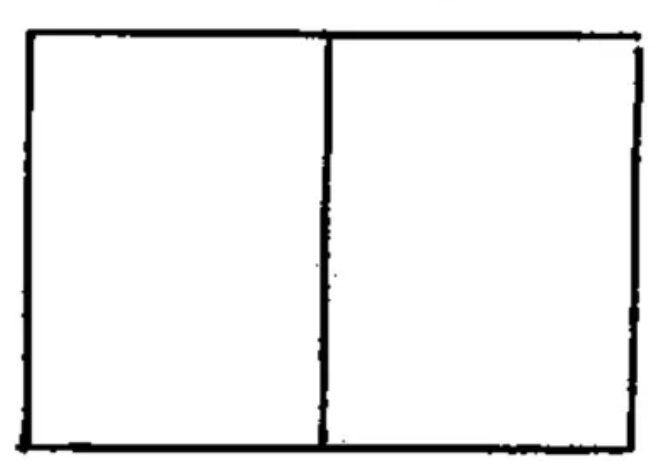
\includegraphics[width=\linewidth]{figs/towel1.png}
  \caption{Moisten the folded towl}
  % \label{x}
\end{subfigure} % \hfill % <-- "\hfill"
\hfill
\begin{subfigure}{.20\linewidth}
  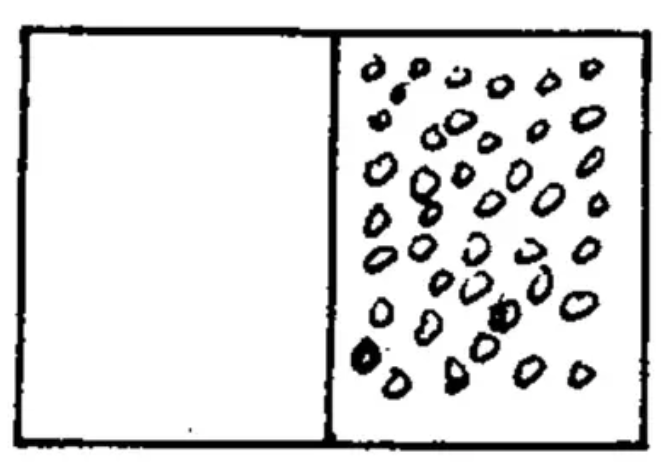
\includegraphics[width=\linewidth]{figs/towel2.png}
  \caption{Sprinkle the seeds on one side}
\end{subfigure}
\hfill
\begin{subfigure}{.20\linewidth}
  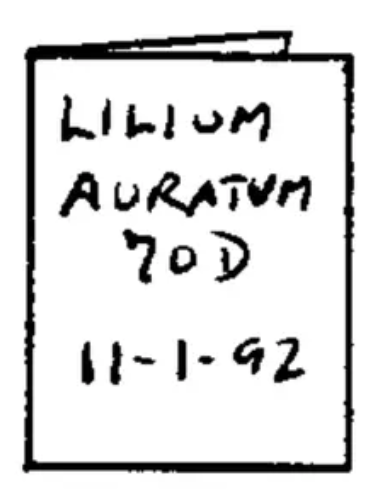
\includegraphics[width=.75\linewidth]{figs/towel3.png}
  \caption{Fold the towel}
  % \label{velcomp}
\end{subfigure}
\hfill
\begin{subfigure}{.20\linewidth}
  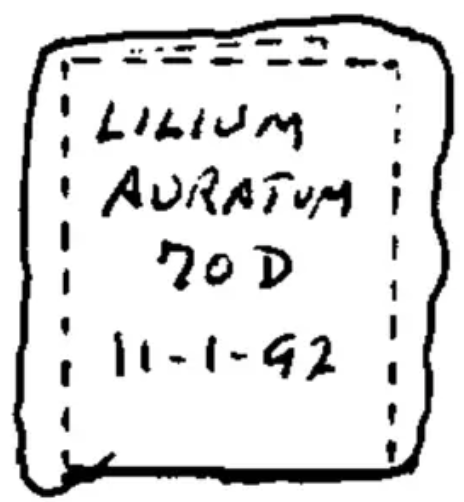
\includegraphics[width=.75\linewidth]{figs/towel4.png}
  \caption{Place in Baggie, fold loosely}
  % \label{estcomp}
\end{subfigure}

\caption{Towel Procedure}
\label{fig:towel}

\end{figure}


A special warning is made about certain brands of paper towels that are
advertised for their softness. These become mushy very quickly. It is important to use
high wet strength paper towels, and the plain white type are preferred. Also a special
warning against Ziploc bags and other polyethylene bags that are of thicker
polyethylene film and are constructed to seal tightly. Polyethylene film is permeable to
oxygen but not water (even though water is the smaller molecule) so that by using the
thinner polyethylene, the permeablility of the film to oxygen helps maintain aerobic
conditions.

The paper towels remain moist for periods of months and only need to be
remoistened at periods of two months or longer. The towels are inspected and the
germinated seeds counted at least once every seven days and as often as each day if
germination is occurring at a rapid rate. If there is debris or other material that starts to
rot, the seeds are transferred to new moist towel. Dead seeds rot in month or two
and are removed. It was usually necessary to transfer ungerminated seeds to a new
towel about every three months as even the ScotTowels ultimately disintegrate. The
edge of a dull knife blade was a particularly convenient instrument for transferring
seeds from one towel to another. Samples of seeds were started at both 40 and 70
and shifted to the alternate temperature every three months.

This method of germinating seeds in moist paper towels was first described in a
talk given by Margery Edgren at an annual meeting of the American Rock Garden
Society, and I am much indebted to the inspiration of this talk. The procedure can be
used to germinate seeds for growing on to plants as described in Chapter 14. It is a
highly efficient procedure for seeds that have extended germinations since watering is
minimal and little space is required. About twenty pads can be stacked in each
Baggie, and about five hundred experiments can be conducted in one cubic foot. I
dread to think of earlier investigators with rows and rows of pots or Petri dishes that
needed almost daily attention.

There was the possibility that chemicals used in processing the paper towels
had an effect on germination. The fact that highly successful germination was
achieved in all but perhaps five or less species out of the nearly 2500 examined
indicates that this was not a factor.

\textbf{Photoexperiments.} The photoexperiments were started in the same way as
the basic procedure except that the seeds were placed on top of the 2.5 x 4.5 inch pad
of moist paper towel. Each moist pad was placed in its own Baggie, and the Baggie
was folded several times as in the basic procedure. -These were placed at a distance
of eight inches under two fluorescent lights. These lights were daylight type, four foot
long, and forty watts each. The lights were timed to provide alternating twelve hours of
light and twelve hours of dark. The effects of light were sometimes complex and
changed by prior treatment as discussed in Chapter 11.

Outdoor Treatment. The outdoor conditions simply consisted of placing the
polyethylene bags containing the towels and seeds outdoors in a shed. The only
important precaution is to prevent any direct sunlight from striking the polyethylene
bags as that would lead to overheating.

\textbf{Gibberelic Acid-3 (GA-3).} The GA-3 experiments started with the same
basic procedure. After opening the third fold and moistening the towel, two inserts
were made before sowing the seeds. The first was a 3 x 3 inch piece of polyethylene
cut from a Baggie. The second was a small piece (2.5 x 2.5 inches) of ScotTowel
folded three times to give a rectangular pad 0.5 x 1.0 inches. This is moistened and
placed on top of the polyethylene. The seeds are placed on top of this inner pad and
one cubic millimeter of 95\% GA-3 is sprinkled on top of the seeds. This amount of GA-3
is about the amount that can be balanced on the 0.5 mm tip of a toothpick using a
type of toothpick that is pointed at both ends. The whole is folded once and placed
inside a Baggie as in the basic procedure. These steps are illustrated by \ref{fig:towel-ga3}.

\begin{figure}[hbt!]

\begin{subfigure}{.20\linewidth}
  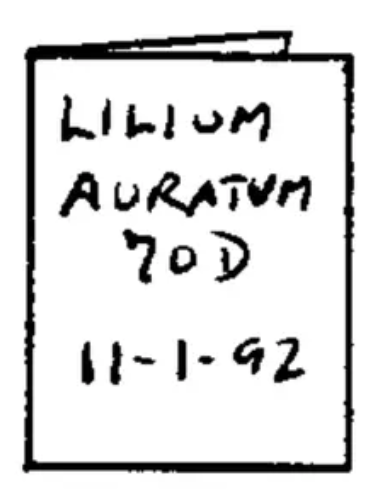
\includegraphics[width=\linewidth]{figs/towel3.png}
  \caption{Towel folded}
  % \label{x}
\end{subfigure} % \hfill % <-- "\hfill"
\hfill
\begin{subfigure}{.20\linewidth}
  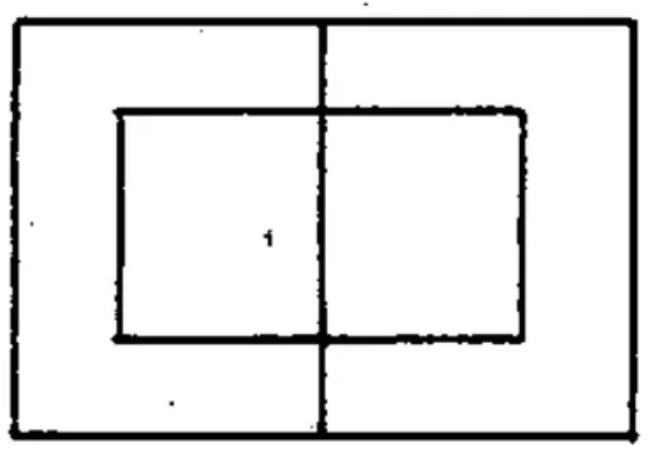
\includegraphics[width=\linewidth]{figs/towel-pi.png}
  \caption{Towel with polyethylene insert}
\end{subfigure}
\hfill
\begin{subfigure}{.20\linewidth}
  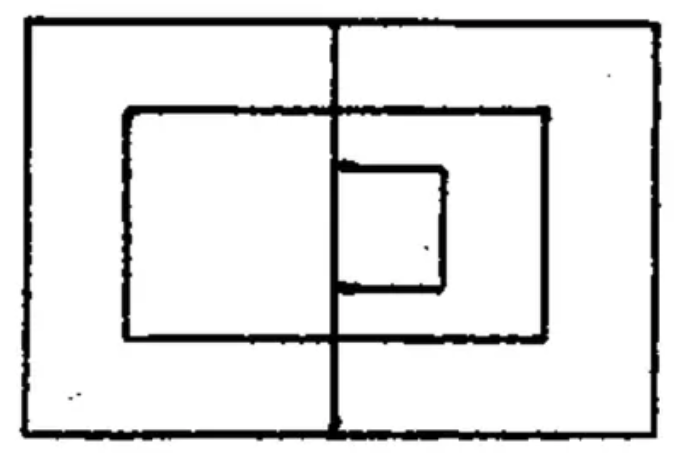
\includegraphics[width=.75\linewidth]{figs/towel-pi2.png}
  \caption{Inner pad inserted, moistened, and ready for seed}
  % \label{velcomp}
\end{subfigure}
\hfill
\begin{subfigure}{.20\linewidth}
  Sow seed, add GA-3, fold, insert in Baggie, and loosely fold as before
\end{subfigure}

\caption{Towel with GA-3}
\label{fig:towel-ga3}

\end{figure}



It was important to adopt reasonably hygienic techniques since some species
such as Evodia danielli were very sensitive to GA-3, and it would not do to
contaminate the work area with GA-3. Everything used to handle the GA-3 was
washed after use.

The beauty of the above procedure is that it does not require any weighing,
volume measurements, or filtering. The experiments take up very little space, and they
can be set up rapidly and examined rapidly. The size of the inner pad is such that it
takes about six drops of water to moisten it and with the one cubic millimeter of GA-3
this works out to be a concentration of about 1000 ppm, the concentrations found to be
about optimum in other work (refs. 9 and 10). By applying the GA-3 to only the inner
pad, the GA-3 is used most efficiently. The moist outer pad serves as a water reservoir
maintaing 100\% relative humidity so that the small inner pad does not dry out. The
amount of GA-3 can be reduced or increased and the time of exposure varied by
simply transferring the seeds from the GA-3 experiment to a fresh moist paper towel. A
further advantage is that there are no solutions of GA-3 that have to be discarded.
Note that reuse of GA-3 solution would lead to uncertainties because of varying
absorption of GA-3 by seed coats as well as the seeds.

A further beauty of the above procedure is that it can be used b y every home
gardener, and it can be used for the growing of plants. As soon as a seed germinates,
it is removed and planted as described in Chapter 14. If there are problems with the
seedlings being weakened by etiolation, the dosages and times of contact can be
adjusted as described in Chapter 12.

\textbf{Washing Seeds in Fruits and Berries.} Seeds in fruits and berries
generally contain germination inhibitors in the pulp and these seeds were \textit{always}
washed and cleaned. The abbreviation WC is used to indicate that the seeds were
washed and cleaned. Some fruits such as those of Euonymus contain inhibitors that
are oil soluble rather than the usual water soluble, and such seeds must be washed
with detergents. This subject is covered in Chapter 8. Generally seeds in fruits have a
channel through the seed coat so that impervious seed coats are virtually never found
although Prinsepia is an exception. Thus germination is not benefitted by physical
treatments of the seed coat. Fruits of a number of Ericaceae such as Vaccinium use
another delay mechanism so that washing is more for convenience than necessity.
Impervious Seed Coats. Certain species use the mechanism of an
impervious seed coat to prevent germination before dispersal of the seed (Chapter 9).
Many treatments have been recommended for such seed, but the \textit{only treatment} that
gives reliable and reproducible (and usually dramatic) effects is to physically produce
a hole in the seed coat.

Such holes in the seed coats were made in several ways. Large seeds could
be rubbed against a file or sandpaper until the endosperm showed. It is advisable to
make this hole away from the embryo to avoid physical injury. With bean shaped
seeds of Fabaceae, this means making the hole on the convex edge of the seed.
Every attempt was made to use this reliable method of making a hole. However, there
were some seeds that were so small that recourse was made to rubbing them between
sandpaper.

Soaking in sulfuric acid has often been recommended for seeds with
impervious seed coats, but I advise against it. First of all the temperatures,
concentrations of sulfuric acid, and times of exposure all have to be worked out for
each separate species. More important sulfuric acid is dangerous to use. Many years
ago there were tragic accidents involving loss of eyesight using sulfuric acid, and this
is one of the principal reasons for requiring safety goggles in all chemistry
laboratories. This is no trivial caution from someone outside the field as I was
internationally known for my work and publications on rates and equilibria in sulfuric
acid.

\section{Results that Appear to be Inconsistent}

There will be the temptation for readers to cite some anecdote that appears to
be inconsistent with the results herein, and the experiments themselves occasionally
gave the appearance of being inconsistent. Five factors were identified that could lead
to such apparent inconsistencies.

Seeds are stored under a variety of conditions. To cite an extreme example,
seeds could be stored in a sealed polyethylene bag. Since polyethylene films do not
transmit water, seeds stored in this way are in effect being stored under conditions of
100\% relative humidity or close to it. Such seed is in effect being stored moist and the
behavior will be that of seeds stored moist not dry.

The dieing of seeds in dry storage is a chemical rate process. It is like
radioactive decomposition. A certain amount dies in each time period. Even after
extended dry storage there may remain a few viable seeds.

A most serious problem is the presence or absence of gibberelin producing
fungi in the medium in which the seeds are planted. Since gibberelins such as GA-3
can have a dramatic effect on germination, this factor must be rigidly controlled to get
consistent results. Fortunately in the present work aseptic conditions were used and
the factor was controlled. Much of the past work reported in the literature used soils
and composts and this factor was not controlled. The uncertainties caused by this
factor places much of the past work under a cloud of uncertaintly. An interesting
anecdotal example involves the rosulate violas of the Andes. English collectors had
brought back seeds of these, but germinations were only rarely observed, and such
germinations could not be correlated with any particular treatment. The presence or
absence of gibberelins was probably the unknown factor.

A minor problem relates to variations in the seeds produced. Rarely species
produce two kinds of seed with different behaviors. There have also been reports that
seeds of a particular species differed when produced from different geographical
areas or from years with different weather patterns. This problem was not actively
investigated, but there were many times that two or more samples of seeds of a
species were obtained from widely different areas and sources. Generally the same
pattern of germination was observed, so I am inclined not to attach much importance to
this factor as a cause of apparent inconsistencies.

The fifth factor is the problem of defining a species. Different strains of a
species could have different germination behavior. In the limit two strains could be
identical in all respects except the nature of their seed germination.
The results herein show that many seeds can be stored for six months or more
in a moist state by careful choice of the temperature for storage. For example Eranthis
hyemalis and Fritillaria acmopetala germinate only at 40 deg. F so that the seeds can
be stored moist for many months at 70. Conversely species that germinate at 70 (and
not 40) could be stored for many months in a moist state at 40. For the many seeds
that cannot tolerate dry storage, it is necessary to develop procedures for storing the
seeds in a moist state.

Seeds can be stored moist by placing them in the moist paper towels, placing
the towel in a polyethylene Baggie, and folding loosely. Commercial seed houses are
urged to start storing and distributing seeds of certain species in the moist state.
A question that has not been investigated is whether the moist storage could be
conducted in sealed systems. It may vary from species to species. If it worked, the
seeds could be sealed in polyethylene packets containing a drop of water. Already
some seed houses distribute some of their seeds in sealed packets (Thompson and
Morgan) so that they are already set up for such procedures. Again it is emphasized
that the feasibility of such distributions in the moist state will have to be established for
each species. Note that thin polyethylene films will transmit oxygen. It may well be
that sealed packets will work with polyethylene films but not other plastic films.

 % 3
\chapter{Rates of Germination}

Although the focus on rates of germination was a unique feature of the present
work, most horticulturists and botanists will be interested only in the gross aspects of
such rates. These gross aspects are now presented, and the correlation with theory is
placed in Chapter 19. In the rate experiments the numbers of seeds that germinated
each day were counted, and the data plotted with the number germinated on the
vertical coordinate and the time in days on the horizontal coordinate. \textit{Four types of
plots were observed} and these are shown in Figures 1-4. The plots apply only to the
cycle in which most of the germination occurred. This was sometimes a 70 cycle and
sometimes a 40 cycle, and it was often preceded by a 3 m cycle at the other
temperature. Sometimes it was preceded by several cycles in a multicycle pattern, but
this was less common.

Figure 1 is characterized by an induction period followed by a linear plot in
which a constant percentage of the original sample germinates each day. The
induction period is a chemical time clock during which some critical chemical process
takes place. The linear rate plot is that of a \textit{zero order} rate process, and the rate can
be conveniently expressed as the percentage that germinates each day (\%Id).
Typically the linear plot held until 80-90\% germination after which a tailing off occurred
as shown by the dotted line. Figure 1 was the commonest pattern observed. The
tailing off is theoretically required, and is not an aberration.

\begin{table}[h!]
\centering

\begin{tabular}{l c c c c}
\multirow{1}{*}[0.1em]{\# Germ} &
  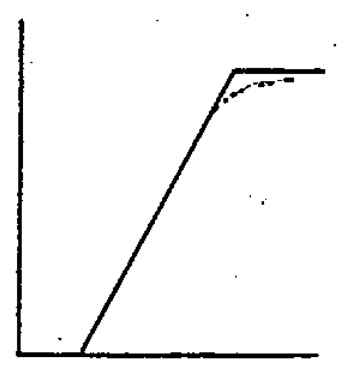
\includegraphics[width=.15\linewidth]{figs/rate1.png} &
  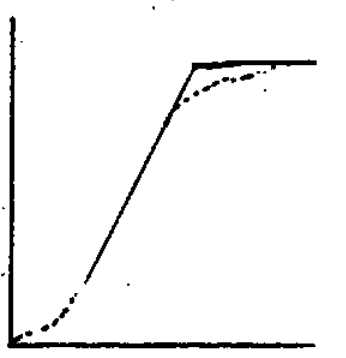
\includegraphics[width=.15\linewidth]{figs/rate2.png} &
  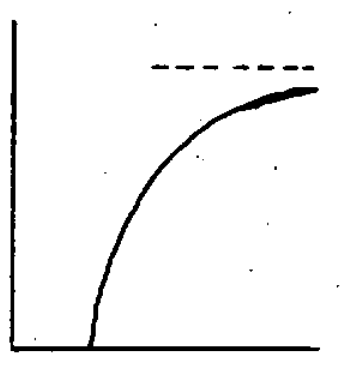
\includegraphics[width=.15\linewidth]{figs/rate3.png} &
  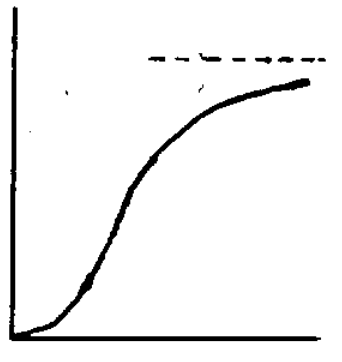
\includegraphics[width=.15\linewidth]{figs/rate4.png} \\
 & \multicolumn{4}{c}{Time in Days} \\
 & Figure 1 & Figure 2 & Figure 3 & Figure 4 \\
\end{tabular}
\end{table}

Figure 2 is like Figure 1 except that there is no induction period. Germination
starts in the first or second day. In the early stages the rate of germination is slowed
down by a deficiencies of water and oxygen in the embryo so that in the first few days
the overall rate depends not only on the rate of the chemical process, but also on the
rates of diffusion of water and oxygen through the seed coat. Within several days the
diffusion rate is no longer a factor, and the linear plot develops. Figure 2 is typical of
many common garden annuals and vegetables. The curve is like an S-shaped curve
at the beginning and at the end and can be mistaken for a true S-shaped curve.

Figures 3 and 4 are analogous to Figures 1 and 2 except that the plot is
rounded curve and of the type where in each time period, a day for example, a
constant fraction of the remaining sample germinates. This type of curve is that of a
\textit{first order} rate process, and the rate is conveniently expressed as the halftime, the
time for half of the seeds to germinate. Thus a half time or half life of five days would
mean that half of the seeds germinated in five days. This first order type of rate should
be familiar because it is the rate law for radioactive decomposition.

Even in the species that required light for germination (Chapter 11),
germinations often followed zero or first order rate laws because of the exact timings
and constant intensity of the light. Even where precise data were not recorded, it was
still possible to record induction times and the range of days or weeks over which 80-
90\% of the germination look place. Thus major changes in rates and induction time
could still be detected. These rates of germination and induction times as well as
other features of the germination have taxonomic significance and serve to
characterize taxa just as much as gross morphology, it was possible in afew examples
to detect two kinds of seeds in the sample by showing that the rate plot was a
composite of two separate rates (see Chapter 19).

Three important generalizations emerged from the rate data. \textit{First} was the
prevalence of induction periods. \textit{Second} was the extremely large changes in rates
with temperature which-were found for the reactions involving conditioning of the
seeds (see Chapter 6). \textit{Third} was the numerous examples of chemical processes that
increased in rate as the temperature was lowered (negative temperature coefficients).

The induction periods shown in Figures 1 and 3 are interpreted as chemical
time clocks involving destruction of germination inhibitors. The phenomenon of an
induction period followed by an \textit{abrupt onset} of germination (or any chemical reaction)
is diagnostic for a chemical clock reaction and the destruction of an inhibitor. It is
unlikely that the patterns in Figures 1 an 3 can be due to delays in diffusion of water
and oxygen through the seed coat, formation of germination promoters, or time
required for an embryo to grow. All of these would lead to a \textit{gradual onset} of
germination.

It might help in understanding chemical time clocks to give an example from
everyday life. Rubber bands can sit in a drawer for a year or more without any
apparent change in outward appearance or any change in their elasticity. One day
cracks start to develop and the rubber band is soon easily ruptured and ultimately
crumbles. The explanation is that raw rubber is rapidly oxidized by oxygen in air in a
complex chain reaction which results in cleavage of the polymeric chains and
crumbling of the rubber to a powder. In the manufacture of rubber \textit{chemical inhibitors}
are introduced into the rubber which block the chain reaction and preserve the rubber.
Ultimately these chemical inhibitors are used up whereupon the oxidative degradation
of the rubber abruptly begins and proceeds rapidly.

It may seem surprising to persons outside the field of physical organic chemistry
that chemical processes of multistep and complex nature can still follow simple rate
laws such as those of a zero order or first order process. The reason has been
understood for some years in physical organic chemistry in terms of a rate determining
(r.d.) step. Generally in a process consisting of a number of steps, one step will the the
slowest. Not only will it limit the rate of the overall process, but it will dictate the rate
law.

One might wonder why seeds that appear to be identical germinate over a
period of time and not all at once. The same question arises for radioactive
disintegration and in fact all chemical processes. It was one of the great triumphs of
science when Boltzmann worked out the theory of this (Boltzmann statistics). The
answer using seeds as an example is that germination requires a particular
conformation of the molecular motion and a particular concentration of energies. The
chance of achieving this for any seed at any moment is statistically determined. To
add a brief personal note, the Noble Laureate George Uhlenbeck gave a course at the
University of Michigan in which he traced the course of Boltzmann's life and the
development of his theories. My wife Virginia was taking the course so I sat in. It was
a wonderful experience, and it gave an invaluable insight into this field.
Incidentally for young people starting out in any career. Take time to broaden
your viewpoints by attending lectures in areas outside of your own. Considerable
selectivity must be exercised to avoid wasting time hearing endless garbage, but the
rewards can be great. It is the cross fertilization of fields that leads to innovation.

 %4
\chapter{Inhibitor Destruction by Dry Storage}

A common misconception is that seeds will germinate if given a little moisture
and a little warmth. This misconception arises because the seeds of about 50\% of all
temperate zone plants can be collected, put in an envelope on the shelf, and
germinated months later when given moisture and warmth. What is often overlooked
is that the period of dry storage on the shelf was essential to the germination. What
happens is that chemical inhibition systems are present initially and these are
destroyed by the drying. This is the commonest mechanism for preventing
germination of the seed before it is dispersed. It is convenient to call these D-70
germinators. Germinators of the D-70 type are predominant in Asteraceae (daisies),
Brassicaceae (mustards), Cam panulaceae (bellflowers), and Poaceae (grasses).

They also predominate in species of agricultural importance, because it was important
to early man to be able to dry store the seed over winter. What evolved in agriculture
was an efficient selection for this type. Most of the common garden annuals are also of
this type. The 50\% of all temperate zone plants that are not D-70 germinators tend to
be avoided and regarded as recalcitrant germinators. The use of the term immediate
germinators for these of the D-70 type is objectionable because they will not
immediately germinate unless given a prior dry storage.

The processes involved in the destruction of germination inhibitors have not
been examined from a chemical standpoint, and in fact have hardly been recognized
as chemical processes in the literature on seed germination. It is planned to determine
if oxygen is required by testing whether these processes can be conducted in sealed
envelopes and anaerobic atmospheres. It will be an exciting area of research in the
future to elucidate the nature of these chemical processes. They may prove to not be
simple destruction of a chemical compound, but rather changes in protein
conformations and changes in membrane structure. These are regarded as ultimately
chemical in nature.

The dry storage requirement and the dramatic effects of dry storage are shown
by some representative data in Table 5-1. The effect of dry storage can be overlooked
if seed is collected from seed capsules in which sufficient drying has already occurred,
particularly in species requiring only a short dry storage period. Dry storage times
have been reported to range from three weeks for barley to sixty months for Rumex
crispus (ref. 12). These timesmust depend on temperature and relative humidity.
However, in the experiments reported these variable were not precisely controlled.
Fresh seed of many 0-70 germinators show two curious behaviors. The more
important one is that if fresh seed is placed in moisture at 70, it seems to be
permanently injured and fails to give significant germination thereafter no matter what
the treatment. This was found to be true for the species in Table 5-1. The second
curious behavior was shown by the Armeria, the five Draba, and the Doronicum in
Table 5-1. Although fresh seed germinated poorly if at all at 70, it germinated fairly
well at 40 albeit slowly. It is as if the germination inhibitors that are so effective at 70
are either not soeffective at 40 or are partially destroyed at 40.

The percent germinations in Table 5-1 were calculated on the basis that the
number of seeds was the number that germinated under the optimum conditions. This
was always at least 60\% and usually 80-90\% of the normal size seed coats.

Many species of the D-70 type grow well and set abundant seed in climates
with moist summers, but few seedlings appear. The explanation is that the seed is
shed in midsummer and encounters summer moisture before the seed has had a
chance to dry. This injures the seed irreversibly. The solution is to collect the geed,
dry store it, and sow after drying. In this way colonies can be maintained.
There are some seeds that seem to germinate immediately at 70 both fresh and
dry stored. An example is Eunomia oppositifolia. It is possible that these are D-70
germinators in which the reuisite dry storage time is very short. Another species with
a related behavior is Centaurea maculosa. The seed germinates immediately at 70 on
being placed in a moist towel so the question arises as to why the seed does not
germinate in the seed capsule, particularly since the ripe seed is held in the seed
capsule for months. An explanation is given in Chapter 9 and involves a tight
receptacle that protects the seed from moisture.

\begin{table}[h!]
\centering

% \begin{tabular}{ |p{3cm}|p{1cm}|p{1cm}|p{3cm}|p{1cm}|p{1cm}| }
\begin{tabular}{|l|c|c|l|c|c|}
 \hline
 Species &
 \multicolumn{2}{|p{2cm}|}{\% Germ, 1 month at 70} &
 Species &
 \multicolumn{2}{|p{2cm}|}{\% Germ, 1 month at 70} \\
 \hline

 & fresh & dry & & fresh & dry \\

\hline
Anemone cylindrica & 4 & 98     & Draba densifolia & 0 & 100 \\
Armeria caespitosa & 15 & 90    & Draba lasiocarpa & 1 & 100 \\
Aster coloradoensis & 0 & 100   & Draba parnassica & 5 & 100 \\
Campanula carpathica & 2 & 85   & Draba sartori    & 5 & 100 \\
Doronicum caucasicum & 10 & 100 & Hesperis matronalis & 0 & 50 \\
Draba aizoon & 0 & 100          & Penstemon grandiflorus & 0 & 50 \\
Draba compacta & 2 & 100        & Townsendia parryi      & 5 & 100 \\
Draba dedeana & 0 & 100         & & & \\
\hline
\end{tabular}

\caption{Comparison of Germination of Fresh Seed Relative to Seed Dry Stored for Six Months at 70}
\label{table:fds}
\end{table}

For species of the D-70 type, two competing chemical reactions are taking place
during the dry storage. One is the destruction of germination inhibitors discussed
above. The second is steady dieing of the seeds. Ultimately all seeds die if dry
storage is prolonged far enough. The situation is best pictured as the \textit{superposition of
two plots}. Both plots have time on the horizontal coordinate. One plot proceeds
upwards from the zero-zero point as time progresses, and this represents the number
of seeds that have become ready for germination due to destruction of the germination
inhibitor. The second plot also starts from zero and is the number of seeds that have
died. The true number of germinatable seeds is the \textit{first plot minus the second plot}.
The resulting curve will go through a maximum so that there is some time when the
number of germinatable seeds maximizes. Fortunately the maximum will be a broad
one as there will be a considerable time period when the two processes approximately
compensate for each other.

In principle it is also possible to have D-40 germinators; That is the seed
requires drying to destroy inhibitors but then germinates at 40. In such species
everything is like the D-70 germinators except that the rate of germination is much
faster at 40 than at 70. However, species that germinated at 40 after dry storage
generally had induction periods of at least six weeks at 40 suggesting that further
germination inhibitors were present that had to be destroyed at 40 in moisture. Thus
the germination patterns were more complex. This type is discussed in Chapter 6.
Most garden annual and vegetables are D-70 germinators. A representative
selection were examined and these are presented here rather than in the data
summary in Chapter 20. Germinations were rapid. Celosia, marigold, portulaca,
radish, and zinnia showed emergence of the radicle in two days. Tomato, bean,
cucumber, watermelon, squash, swiss chard, corn, sweet pea, sweet William, and
candytuft showed emergence of the radicle in three days. Four to five day induction
periods were shown by alyssum, lobelia, nasturtium, and carrot. The rates were : -
approximately first order for marigold, radish, squash, sweet William, swiss chard,
watermelon, and zinnia with half lives of one to two days. The rates were
approximately zero order for candytuft, carrot, and sweet pea with rates of 25-50\%/d.
In general the germination rates were negligible at 40, but alyssum germinated at the
same rate and ind. t at 40 as at 70 and with candytuft, carrot, nasturtium, radish, sweet
william, and swiss chard the germination rate was the same but the ind??t was two to
three times longer.

The number of genera studied could have been much increased by including
studies on numerous garden annuals and Asteraceae. However, these are almost
invariably 0-70 germinators (Vernonia in Asteraceae is an exception), and were not
studied unless there was some reason for anticipating unusual behavior.

 % 5
\chapter{Inhibitor Destruction by Moist Conditions}

\textbf{Destruction of the inhibiting system takes place at 40.} In many
species the germination inhibitors are destroyed simply by exposure to moisture.
There is an induction period before germination begins. After the induction period
there is a sudden onset of germination. This pattern can occur at either 40 or 70.
Some examples of this behavior for species germinating at 40 are shown in Table 6-1.
This group is a problem only because it has not been generally recognized that many
species germinate exclusively at 40.

A pattern that requires somewhat more planning to achieve germination are
those in which the inhibiting system is destroyed by exposure to three months moist at
40 followed by germination on a shift to 70. These will be termed 40-70 germinators.
Some examples of these are given in Table 6-2. This pattern is well known, but the
period at 40 has traditionally been spoken of as a period required to "break
dormancy." It should be clear from the discussion in Chapters 1 and 2 that this is a
\textit{conditioning period} and a period of \textit{maximum metabolic activity} for those chemical
processes that destroy the inibiting system. It is only a dormant period in respect to
vegetative growth.

The destructions of the inhibitor systems at 40 are rate processes and will be
different for each species. Minimum times for the low temperature cycle for seeds
have been reported to be twelve hours for wheat, seven days for Poa annua, fourteen
days for Delphinium ambiguum, and six months for Crataegus mollis (ref. 13). Data
given below in Table 6-3 for Nemastylis acuta shows that the time for this species is
about three months.

The destructions of germination inhibitors in seeds at 40 are clearly related to.
the destruction of growth inhibitors which occurs during winter in \textit{vegetatively dormant}
flower buds and vegetative buds of deciduous trees and shrubs as well as \textit{vegetatively
dormant} bulbs and tubers. A similar period of about three months at temperatures
around 35-42 degrees F is needed in order for vegetative growth to occur on shifting to
warmer temperatures. The similarity or possible identity with the chemical processes
in seeds remains for future investigators to determine. In any event such periods
should be called conditioning periods and not breaking dormancy unless one
specifies that one is speaking of dormancy only in regard to vegetative growth.
The fact that these inhibitor destruction reactions occur at 40 but not 70 requires
that the rates of the processes increase enormously in lowering the temperature from
70 to 40. Enzyme reactions and protein and membrane restructuring have a special
capacity for these unusual negative temperature coefficients, and the theory of this is
explained in Chapter 19.

The data in Tables 6-1 and 6-2 represent two limiting situations. The inhibitors
are destroyed at 40 in both, but in the examples in Table 6-1 germination occurs at 40
whereas in the examples in Table 6-2 germination is so slow at 40 relative to the
germination rate at 70 that a shift to 70 is necessary to achieve germination.
There are intermediate situations where the rate of germination at 40 is
significant, but the rate at 70 is much faster. Nemastylis acuta illustrates this situation
and the data appear in Table 6-3. The inhibitor destruction requires about three
months at 40. At this time there is the option for either allowing a slower germination to
proceed at 40 or a faster germination to proceed at 70 by shifting the seed to 70.
Analysis of the data shows that the germination rate at 70 is 2.3 times faster than at 40.
This temperature coefficient is in the range typical for most chemical processes. Note
that the grower will fail if the seeds are kept moist at 40 in the dark, because after three
months they will start to germinate and die for lack of light. Incidentally, Nemastylis
acuta has beautiful two inch wide sky blue flowers with Tigridialike pleated foliage. It
is one of the most beautiful of hardy bulbs and is little known in horticulture.

\textbf{Destruction of the inhibiting system takes place at 70.} This situation
also generates two limiting germination patterns. In one pattern there is a long
induction period at 70 followed ultimately by germination at 70. The interpretation is
that inhibitors are destroyed at -70 and that the germination itself is faster at 70. In the
other limiting pattern the germination inhibitors are destroyed at 70, but germination
occurs only at 40 so that after the inhibitors have been destroyed at 70, the seeds must
be shifted to 40 in order for germination to occur. Species with this pattern are called
70-40 germinators. This type of pattern has not been explicitly recognized in the
literature, and it was a surprise to find that there were comparable numbers of 70-40
and 40-70 germinators.

Following is a list of species in which germination occurs at 70, but only after an
induction period. This list is restricted to species where the induction time at 70 was
two weeks or longer since this length of time makes it reasonably certain that
germination inhibitors were present. The induction is given in weeks (w) in
parentheses after the name of each species. Aucuba japonica (5 w), Centaurium
erythrosa (2.5 w), Clematis integrifolia (6 w), Clematis pitcheri (4 w), Clematis recta (8
w), Clematis viorna (8 w), Cortusa matthioli (3 w), Cortusa turkestanica (3 w),
Delosperma cooperi (4 w), Eritrichum howardi (4 w), Haberlea rhodopensis (4 w),
Jankae heldrichii (4 w), Leucojum vemum (8 w), Lilium auratum (3 w), Lilium
canadense editorum (7 w), Lilium canadense flavum (7 w), Lilium cernuum (6 w),
Lilium concolor (8 w), Lilium davidi (8 w), Lilium maximowiczii (8 w), Paeonea
officinalis (12 w), Paeonea suffruticosa (12 w), Podophyllum emodi (5 w), Prunus
armenaica (5 w), Silene polypetala (12 w), Silene regia (12 w), Thlaspi bulbosum
(6 w), Thlaspi montanum (6 w), and Thlaspi rotundifolia (6 w).

Table 6-4 lists those species that were straightforward 70-40 germinators.
Examples that had additional complexities are not listed here, but are of course
described in Chapter 20. Note that usually the germination was completed rapidly
over a time span of one to three weeks and this was shorter than the induction times.
There was a minor difference in the species that germinated at 70 relative to the
species that germinated at 40. Where germination occurred at 70, development of
photosynthesizing cotyledons or leaves soon followed. Where germination occurred
at 40, sometimes cotyledons or leaves developed at 40 as in Brodiae congesta and
Eranthis hyemalis, but more commonly only the radicle developed at 40, and a shift to
70 was required for leaf development.

In rare examples either dry storage of the seed for six months at 70 or
subjecting the seed to three months moist at 40 were equally effective in destroying
the germination inhibitors. In Eupatorium urticaefolium germination at 70 was 95\%
complete in 2-5 days after the three months at 40 and 95\% complete in 5-10 days after
the dry storage. The slightly longer times in the latter were due to time required for
water transport in the freshly moistened seed.

Up to now it has been emphasized that inhibitor destruction under moist
conditions virtually never occurred at both 40 and 70. Anemone baldensis is
possible exception in that germination occurred at both 40 and 70 and with significant
induction times. Seed sown at 40 had an induction time of 44 days and a rate of
germination of 4.0\%/d. Seed sown at 70 had an induction time of 18 days and a
germination rate of 5.1\%/d. These values are for fresh seed. As with Eupatorium
urticaefolium, dry storage removed most of the inhibition so that germination at 70 was
speeded up and was 95\% complete in 10-15 days.

A major difference was present between the 40-70 germinators and the 70-40
germinators. In the 40-70 germinators germination took place immediately after the
shift to 70 so that there was usually no significant induction period at 70. In the 70-40
germinators germination took place at 40 usually after a significant induction period,
and this induction period was followed by relatively rapid germination over a period of
two to three weeks. This is interpreted to mean that there was a second set of
germination inhibitors that had to be destroyed at 40. This leads us into the concept of
two or more sets of germination inhibitors which is the subject of the next chapter.

\begin{table}[h!]
\refstepcounter{table}

\begin{center}
Table \thetable. Inhibitor Destruction at 40 Followed by Germination at 40 (a,b)
\end{center}

\begin{tabular}{|l|l|l|}
\hline
Species & Induction time & Germination rate \\
\hline
Allium albopilosum & 5 weeks & 85\% in 5-13 weeks \\
Allium moly & 9 weeks & 90\% in 9-11 weeks \\
Calandrinia caespitosa & 7 weeks & 40(33\%)-70(29\% in 6-10 days)(c) \\
Camassia leichtlinii & 5 weeks & 100\% in 5-14 weeks \\
Chaenomeles japonica & 7 weeks & 86\%, \%5/d \\
Disporum lanuginosum & 7 weeks & 100\% in 8th week \\
Erythronium citrinum & 10 weeks & 40(65\%)-70(35\% in 1-2 days)(c) \\
Erythronium hendersoni & 8 weeks & 93\% in 8-12 weeks \\
Euonymus bungeana & 5 weeks & 90\% in 6th week \\
Fritillaria acmopetala & 9 weeks & 40(45\%)-70(23\% in 2-6 days)(c) \\
Fritillaria persica & 8 weeks & 97\%, ind. 54 days, 8\%/d \\
Gladiolus anatolicus & 7 weeks & 90\% in 7-9 weeks \\
Gladiolus imbricata & 7 weeks & 90\% in 7-9 weeks \\
Gladiolus kotschyanus & 6 weeks & 90\% in 6-12 weeks \\
Hebe guthreana & 7 weeks & 96\%, ind. t 48 days, 4\%/d \\
Iris bracteata & 8 weeks & 90\% in 9th week \\
Iris germanica & 7 weeks & 40(31\%)-70(31\% in 1-6 days)(c) \\
Iris magnifica & 10 weeks & 30-100\% in 10-12 weeks \\
Kirengoshima palmata & 12 weeks & 90\% in 12-16 weeks \\
Lonicera sempervirens & 7 weeks & 100\%, ind. t 50 days, 3\%/d \\
Parrotia persica & 11 weeks & 90\% in 12th week \\
Penstemon glabrescens & 5 weeks & 84\% in 5-12 weeks \\
Rosa multiflora & 5 weeks & 26\% in 5-7 weeks \\
Saponaria caespitosa & 9 weeks & 87\% in 9-12 weeks (dry stored seed) \\
Scilla hispanica & 9 weeks & 32\% in 10th week \\
Zigadenus fremonti & 6 weeks & 92\% in 6-9 weeks \\
\hline
\end{tabular}

(a) It is important to remember that these species gave no germination when
sown at 70 and kept at 70. Where the percent germination was low, it was because of
a predominance of empty seed coats and not because there was further germination
at a later date.

(b) The Table includes only those species where the induction time was five
weeks or longer since it was felt that these were the clearest examples of an induction
period.

(c) Probably germination would have been completed at 40 if more time had
been given. These are examples where the germination rate is much faster at 70 than
at 40.

\end{table}

\begin{table}[h!]
\refstepcounter{table}
\begin{center}
Table \thetable. Inhibitor Destruction at 40 Followed by Rapid Germination on Shifting to 70
\end{center}
\par

\begin{tabular}{|l|l|}
\hline
Species & Germination rate after the shift to 70 \\
\hline
Aesculus hippocasteanum (a) & 100\% in 1-7 days \\
Aesculus pavia & 100\% in 1-7 days \\
Allium tricoccum & 95\%, largely in 10-13 weeks \\
Aquilegia formosa & 50\% in 14-42 days \\
Asciepias tuberosa & 100\% in 2-7 days \\
Asimina triloba & 76\% in 2-35 days \\
Aureolaria virginica & 30\% in 5-24 days \\
Campanula altaica & 68\% in 4-14 days \\
Ceanothus americana & 28\% in 1-21 days \\
Cercidiphyllum japonicum & 50\%, ind. t 2 days, 10\%/d \\
Cornus nuttailli & 40\% in 8-10 days \\
Diospyros virginiana & 60\% in 7-28 days \\
Dodecatheon jeffreyi & 90\% in 1-5 days \\
Dodecatheon media & 92\% in 1-3 days \\
Eupatorium purpureum & 90\% in 3-5 days \\
Ilex japonica & 87\% in 90\% in 1-2 days \\
Myrica pennsylvanica & 85\% in 1-2 days if wax was removed from seed \\
Phytolacca americana & 80\% in 5-16 days if seed was washed and dry stored \\
Primula intercedens & 43\% in 6-10 days if seed was dry stored \\
Primula japonica & 100\% in 2-4 days if seed was dry stored one month \\
Primula parryi & 32\% in 4-42 days \\
Rhamnus caroliniana & 98\% in 4-7 days \\
Ruellia humihis & 33\% in 3-9 days (rest of the seed rots quickly) \\
Trillium albidum & 100\% in 2-4 days \\
Trohlius acaulis & 70\% in 6-10 days \\
Vernonia novaboracensis & 100\% in 2-4 days \\
Viburnum tomentosum & 50\% in 1-26 days \\
Vitis vulpina & 76\% in 4-6 days \\
\hline
\end{tabular}

\hfil

(a) With large fleshy seeds like this species, there is apparently sufficient
moisture in the seed itself so that dry storage at 40 destroys the inhibitors as effectively
as 3 m moist at 40. Although 6 m dry storage at 40 was used, it is likely that 3 m would.
have been equally effective.

\label{table:id40}
\end{table}

\begin{table}[h]
\refstepcounter{table}
\begin{center}
Table \thetable. Inhibitor Destruction at 40 Followed by Germination at Either 40 or 70 for
Nemastylis Acuta
\end{center}
\par
\begin{tabular}{|l l|l|l|l|l|l|}
\hline
Time in months (at 40)        & 1 & 2 & 3    & 4    & 4.5     & 5 \\
\hline
Percent germination           & & & & & & \\
\quad seed kept at 40         & 0 & 0 & 0    & 38\% & 58\%    & 72\% \\
\quad seed shifted, to 70 (a) & 0 & 0 & 44\% & 92\% & 90\%(b) & 90\%(b) \\
\quad seed kept at 70         & 0 & 0 & 0    & 0    & 0       &  0 \\
\hline
\end{tabular}

\hfil

(a) The shift to 70 was made after the time at the head of the column. The
germination at 70 was rapid and was completed in 2-7 days. The value of 44\% at the
end of the three months at 40 is very sensitive to the exact conditions, and values
ranging from 40-80\% were observed. This is because the inhibitor destruction
reaction is just at the point of being completed.

(b) These values include the seeds that had germinated earlier at 40.

\label{table:acuta}
\end{table}

\begin{table}[h]
\refstepcounter{table}
\begin{center}
Table \thetable. Inhibitor Destruction at 70 Followed by Germination at 40 (a)
\end{center}

\par
\begin{tabular}{|l|l|}
\hline
Species             & Germination rate at 40 after 3 months at 70 \\
\hline
Anemone blanda      & 75\%, ind. t 63 d, 3\%/d \\
Actaea pachypoda      & 85\% in 5-8 w       \\
Actaea spicata      & 88\% in 4-7 w         \\
Anemone blanda      & 75\%, ind. t 63 d, 3d \\
Chionodoxa luciliae & 50\% in 12th w        \\
Cimicifuga: racemosa & 100\% in 3-6w        \\
Claytonia virginica &  79\% in 7th w        \\
Clematis alpina     & 80\% in 5-11 w        \\
Clematis maculata    & 100\% in 4-8w        \\
Colchicum autumnale  & 33\% in 6th w        \\
Colchicum luteum     & 58\% in 0-3 w        \\
Corydalis lutea     & 70\% in 10-12 w       \\
Crocus speciosus     & 86\% in 3-5 w        \\
Delphinium glaucum     & 25\% in 4-6w       \\
Eranthishyemalis       & 100\% in 8-9w      \\
Erythronium americanum & 60\% in 10-12w (b) \\
Erythronium revolutum  & 33\% in 12th w     \\
Fritillaria thunbergii & 50\% in 5-7w \\
Galanthus elwesii & 45\% in 5th w \\
Galanthus nivalis & 45\% in 2-5 w \\
Helleborus niger & 93\% in 9th w \\
Helleborus orientalis & 100\% in 5-10 w \\
Hyacinthus orientalis & 100\% in 6-8w \\
Iris albomarginata & 50\% in 7-12 w \\
Isopyrum biternatum & 5\% in 8-11 w \\
Ligustrum abtusifolium & 4\% in 2-12 w \\
Lilium pardalinum & 0\% in 2nd w \\
Lilium parvurn & 90\% in 2nd w \\
Lilium shastense & 90\% in 2nd w \\
Lilium washingtonianum & 61\% in 3-12 w \\
Melampyrum Iineare & 55\% in 4-8w \\
Scilla campanulata & 75\% in 3-11 w \\
Scilla tubergeniana & 100\% in 3-5 w \\
\hline
\end{tabular}
\par
(a) No further germination occurred unless noted.

(b) Germination was 100\% after six cycles.
\label{table:g7040}
\end{table}

 % 6
\chapter{Two or more Inhibiting Systems}

Many examples were found where there were two or possibly more sets of
inhibiting systems, and each set required different conditions for destruction. Eranthis
hyemalis is an excellent example of this and was studied in detail. Eranthis has to be
one of the great horticultural treats. In late March great drifts of the yellow buttercups
carpet the woods and field, and the air is filled with their intense honey fragrance. On
warm days the honey bees and butterflies that have hibernated come for their first
feast after the long winter. As a result there is always a rich crop of seed that ripens in
the first week of May.

Eranthis hyemalis has one inhibiting system that is destroyed at 70 and another
that is destroyed at 40, and they must be destroyed in that order. The seeds are placed
in moist towels at 70 as soon as they are ripe in May. After 3 m at 70, the seeds are
shifted to 40. After an induction period of exactly 55 days (note the length),
germination begins and proceeds at a rate of 250/old (note the high rate) so that
germination is over 90\% complete in tour days. Over the following month the radicle
develops and the cotyledons start to open. The seedlings have to grow under
relatively cool conditions as this species is programmed to go dormant if temperatures
above 70 persist. As a result shifting the seedlings directly to 70 leads to their dieing
off. Of course the simplest procedure for a gardener is to broadcast the seed as soon
as collected and in a few years large colonies will develop.

If the seed is subjected to a three cycle pattern starting at 40, the results are 40-
70-40(90\% in 55-59 d). The first three months at 40 have absolutely no effect on the
percent germination, the induction period, or the rate of germination and is truly a
dormant state with little or no metabolic activity. The-three months at 70 in either the
70-40 or 40-70-40 pattern is again a time of metabolic activity inside the seed despite
the absence of any outward signs, and chemical reactions are occurring that are
absolutely essential for the germination in the following cycle at 40. -
The importance of low temperature metabolism has been a dominant theme in
this book. In Eranthis hyemalis the germination, development of radicle, and
expansion of cotyledons takes place rapidly at 40 and will not occur at 70. It is evident
that in the plant kingdom neither germination inhibitor destruction nor growth of roots
and leaves are restricted to either high (70) or low (40) temperatures.

A number of experiments were conducted on the seeds of Eranthis hyemalis to
better understand the chemical reactions and metabolism in the three months at 70. If
the period at 70 is shortened from three months to two months, germination at 40 is
seriously affected. The induction time lengthens to 60-70 days and the germination
rate drastically slows down. It is evident that two months is not long enough for the
requisite chemical changes to be completed. If the time at 70 is lengthened from three
months to six months, the germinatiion behavior at 40 is identical to seeds given three
months at 70 showing that the additional three months were a period of inactivity.
However as the time at 70 is further increased, the induction period starts to lengthen
and the germination rate declines showing that irreversible injury and death is
beginning to occur. Although it was not examined, it is likely that seedlings from non-
optimum conditions for germination will be weaker and perhaps fail to develop. In the
40 .70-40 treatment the effect of lengthening the first three months period at 40 was not
examined. Presumably it could be lengthened to apoint where irreversible injury
appeared.

Seed of Eranthis hyemalis will not tolerate dry storage for six months at either
70 or 40 and seed so treated is dead. In the future if seeds of Eranthis are to be stored
and distributed, it is recommended that they be stored in moist towels at 70 or 40 and
distributed in this state. As it stands now, all the seed distributed commercially or by
seed exchanges is DOD (dead on delivery).

Eranthis hyemalis produces only the pair of cotyledons in the first year of
growth. Among dicotyledons this behavior is uncommon, but it has been found in
Oxytropis williamsii in Fabaceae; Anemonastrum, Clematis albicoma, and Eranthis in
Ranunculaceae; Dodecatheon amethystinum and Dodecatheon media in
Primulaceae; and Skimmia japonica in Rutaceae.

Suppose that in Eranthis hyemalis the germination had been fast at 70 and zero
at 40. The seed would then have required three months at 70, three months at 40, and
finally germination after a shift to 70. Now Eranthis does not do this, but it illustrates
that the inhibitor destruction pattern for 70-40 germinators can be the same as for 70-
40-70 germinators, and this introduces us to the world of multicycle germinators.
Many species did not germinate until after two or more alternating three month
cycles. These are termed multicycle germinators. While more work is needed to
conclusively demonstrate that two or more sets of inhibitors were present, this is the
most likely interpretation (although it is not readily distinguished from situations where
the rate of germination is very slow at the temperature of the second cycle). These
multicycle germinators were of two types. In the simpler type germination was
reasonably confined to three or four cycles. Actaea rubra and Iris graeberiana were
40-70-40 germinator and Cercis chinensis and Erythronium mesochorum were largely
70-40-70 germinators. Delphinium tricorne was a 70-40-70-40 germinator. In others
the germination dragged on cycle after cycle, usually with a little germination in the first
two cycles with the majority in subsequent cycles.

There is always the question as to whether longer cycle times, different
temperatures, or some other untried factor would have speeded up the process. In fact
some species that were initially observed to have long drawn out germination over
many cycles were later found to germinate readily in outdoor treatment, in various
phototreatments, or when treated with gibberelins. Some Iris have these long drawn
out germinations, particularly the Juno and Oncocyclus. Attempts were made to speed
up germination by subjecting the seeds to month long soakings in water, by removing
the brown seed coats, by light, and by treatment with gibberelin, all without effect.
Combinations of wet and dry cycles and temperatures over 100 were not tried, and
these merit exploration since these species come from regions with hot dessicating
summers.

Table 7-1 summarizes the data on some three cycle germinators. Table 7-2 lists
some species with even longer drawn out germinations. Sometimes these long drawn
out germinations were associatedwith stepwise germination in which the radicle
developed in one cycle and the leaves in a following cycle as in Jeffersonia diphylla
and dubia. One obvious survival advantage of such long drawn out germinations is
that if a particular year had inclement weather, there would be new seedlings for the
following years. However, the way Oncocyclus Iris seed will remain in a firm and
healthy condition for years suggests that some key factor needed for germination is as
yet undiscovered.

\begin{table}[h]
\refstepcounter{table}
\begin{center}
Table \thetable. Species Whose Germination Is Predominantly in the Third or Fourth Cycle
\end{center}

\par
\begin{tabular}{|l|l|}
\hline

\multicolumn{2}{|c|}{70-40-70 Germination } \\
\hline
Acer spicatum & 70-40-70(28\% in 3-8 weeks) \\
 & 40-70-40-70(9\%) \\
Chionanthus virginica & 70-40-70(54\% in 5-9 weeks)-40-70(29\% in 5-7 weeks) \\
 & 40-70(7\%)-40-70(54\% in 4-8 weeks) \\
Corylus cornuta & 70-40-70(86\% in 1-3 weeks) \\
 & 40-70(14\%)-40-70(57\% in 1-6 weeks) \\
Dicentra spectabilis & 70-40(12\%)-70(28\% in 3-9 days) \\
 & 40(21\%)-70(5\%)-40(12\%)-70(1 \%) \\
Dionysia involucrata & 70-40-70(50\%) \\
Iris hookeri & 70-40-70(100\% in 2nd week) \\
Lilium chalcedonicum & 70-40-70(100\% in 5-7 weeks) \\
Paris quadrifolia & 70(6\%)-40-70(69\% in 7-12 weeks) \\
 & 40-70-40-70(66\% in 7th week) \\
Passiflora edulis & 70-40-70(81\% in 4-6 weeks) \\
 & 40-70-40-70 none \\
\hline
\multicolumn{2}{|c|}{ 40-70-40 Germination } \\
\hline
Iris graeberiana      & 40-70-40(90\% in 6-11 weeks) \\
 & 70-40(45\% in 10th week)-70-40(18\% in 9-12 weeks) \\
\hline
\multicolumn{2}{|c|}{ 40-70-40-70 Germination } \\
\hline
Stylophorum diphyllum & 40-70-40(4\%)-70(69\% in 1-15 days) \\
\hline
\multicolumn{2}{|c|}{ 70-40-70-40 Germination } \\
\hline
Viburnum dilitatum    & 70-40-70-40(70\% in 2-5 weeks) \\
Viburnum opulis       & 70-40(3\%)-70-40(62\% in 2-8 weeks) \\
\hline

\end{tabular}
\label{table:s34}
\end{table}

\begin{table}[h]
\refstepcounter{table}
\begin{center}
Table \thetable. Examples of Extended Multicycle Germinations
\end{center}
\par
\begin{tabular}{|l|l|}
\hline
Allium karataviense & 70-40-70(6\%)-40(30\%)-70(10\%)-40(14\%)-70(6\%) \\
                    & 40-70-40(3\%)-70(14\%)-40(2\%)-70(14\%) \\
Eleaganus umbellata & 70-40(24\%)-70(25\%)-40(6\%)-70(18\%) \\
Fritillaria pallida & 40-70-40-70(20\%)-40(60\%) \\
Iris acutiloba & 70-40-70(10\%)40-70-40-70(70\%) \\
Jeffersonia dubia & 70-40(4\%)-70-40(2\%)-70(4\%)-40(14\%)-70(24\%)-40(6\%) \\
Rhodotypos tetrapetala & 70-40(44\%)-70(16\%)-40(12\%) \\
                       & 40(14\%)-70(24\%)-40-70(14\%)-40(11\%)-70(3\%) \\
Taxus baccata       & 70-40-70(1\%)-40-70(28\% in 5-15 days)-40-70 \\
                    & 40-70-40-70(11\% in 1-16 days)-40-70(26\%)-40-70(10\%)-40-70(8\%) \\
\hline
\end{tabular}
\label{table:smc}
\end{table}

 % 7
\include{ch-fruit} % 8
\chapter[Physical Mechanisms]{Physical Mechanisms for Inhibiting Germination}

Many Fabaceae (legumes), a few Malvaceae, and a few other species use
impervious seed coats as the mechanism for preventing germination before the seed
is dispersed. It is not clear whether the mechanism operates by excluding water or
oxygen or both, but what is clear is thit grinding whole through the seed coat
produces a dramatic effect with the seeds germinating in a few days after puncturing
the seed coats and placing in moist media. With seeds large enough to be held in
pliers, the seed is held against a grinding wheel until the interior of the seed just
shows. Alternatively the seeds can be filed or sawed with a hacksaw until the
endosperm shows. The seeds can also be held in pliers or tweezers and ground
against sandpaper or a file. It was best to grind against the convex side of the seed to
avoid any mechanical damage to the undeveloped radicle. The dramatic effects of
such pretreatment of the seed is shown in Table 9-1 at the end of this Chapter.
The favorable effects on germination induced by various grinding and abrasion
procedures has long been known. This subject is treated in recent books under the
title scarification. This term should be promptly abandoned because producing a scar
on the seed coat surface has no effect. Only the formation of a true water channel and
hole through the seed coat will reliably and reproducibly give immediate germination.
Thompson and Morgan use the words nicking, pricking, and filing in their catalog.

Puncturing has been used herein. Obviously we are searching for a suitable word.
It has often been recommended to soak seeds of this type in hot water or to pour
hot or boiling water over the seeds. An example taken from the Thompson and
Morgan catalog is to immerse seeds of Mimosa pudica in 140 deg. F water for twenty
minutes. I have verified the effectiveness of this procedure. Prof. Roger Koide at
Pennsylvania State University has found that ten minutes in water at 140 is effective
for Abutilon theophrasti. The Thompson and Morgan catalog recommends soaking in
hot water for a number of species, and it can be inferred that these have impervious
seed coats. There are two problems with these hot water treatments. The optimum
conditions vary with each species and have to be determined, and the results are
generally less effective than physically producing the hole in the seed coat as shown
below by the results with Gymnocladus dioica.

The hot water treatments work because the heat causes expansion of the seed
coats. This causes microfissures to form and in effect a hole has been produced in the
seed coat. The extensive studies described below on Gymnocladus dioica are all in
accord with this interpretation. Inferences in the literature that the soaking softens the
seed coat are incorrect, although the seed coats then soften in a day or two due to
enzymes secreted by the activated seed.

Gymnocladus dioica seeds were treated for five and ten minutes at ten degree
temperature intervals ranging from 120 to 180 deg F. Eight seeds were used at each
condition. The number germinated in the five minute treatments were 3, 4, and 4 at
120, 130, and 140. The number germinated in the ten minute treatments were 2, 4,
and 2 at 1 .20, 130, and 140. The seeds were all killed at 150-180. Increasing the time
from five minutes to ten minutes increases the number of seeds killed with no added
stimulation of germination. Samples of eight seeds were then given fifteen second
treatments at 150, 160, and 170. The numbers of seeds germinated were 4, 1, and 1.

Clearly the fifteen seconds at 150 was just enough to expand the seed coat without
cooking the seed inside. However, \textit{none of these treatments gave over 50\%
germination which is less effective than the 100\% germination effected by physically
producing a hole in the seed coat.} All germinations were in two to ten days.
Freezing and thawing have often been recommended for inducing germination
of seeds. In general the effect of freezing and thawing is a myth, and true freezing and
formation of ice crystals within the seed would be fatal. However, temperature
oscillations generally serve to open microfissures. Albizziajulibrissin exemplifies this
effect. Seed subjected to outdoor treatment over one winter gave 24\% germination in
the following April and first week of May showing that microfissures had been opened
in 24\% of the seeds. There was additional germination after a second winter. -There
was no germination in controls held at 40 or 70. In nature it may take several years for
a significant number of seeds to form the requisite microfissures, and it has been
observed in the garden here that Kentucky Coffee Tree (Gymnocladus) seeds do not
germinate for several years after falling. Drying can also induce fissures in the seed
coats, and this was evident in Honey Locust and Kentucky Coffee Tree, Table 9-1.

Many other treatments have been recommended, but all of them suffer in that
they give results that lack uniformity and reproducibility, and they require extensive
study to define optimum conditions. These methods include rubbing between
sandpaper, heating until a few seeds pop, centrifugal devices that throw the seed
against abrasive surfaces, and immersion in concentrated sulfuric acid. This last
procedure is particularly hazardous as was described in Chapter 3.
Although impervious seed coats are characteristic of Fabaceae, many species
in this genus have microfissures already present in varying degrees. Peas and beans
of the vegetable garden germinate readily enough without pretreatment. Hedysarum
cephrolotes, Lathyrus latifolius, Lespedeza bicolor, and Wisteria chinensis germinated
immediately at 70. Baptisia australis, Cercis canadensis, Cercis chinensis, and
Indigofera heteranthera showed some increase in rate of germination with
pretreatment but the minor gain in rate was overbalanced by the increase in rotting
which lowered the overall percent germination (Chapter 20). Coronilla varia, Genista
subcapitata, Lotus corniculatus, and a number of Astragalus and Oxytropis would
probably have benefitted from a hole in the seed coat, but the experiments were not
conducted and modest amounts of germination were achieved without puncturing.

Finally some species with impervious seed coats produce a significant
percentage of seeds that are imperfect in that they already have a miprofissure. These
germinate immediately, but the remaining will not germinate until a hole is produced in
the seed coat. The data on Melilotus alba are an excellent example of this effect.
As might be expected it is species with impervious seed coats that have the
longest life in dry storage. This is discussed in Chapter 13.

The presence of a hard bony seed coat does not indicate the need for
mechanical pretreatment, and in fact a number of very hard and bony seeds have a
water channel through the seed coat. Examples are Cornus Prunus, and Rosa
multiflora. careful examination of these seeds will reveal the cleavage between the
two halves, and producing a hole in the seed coats does not initiate germination.
Conversely a soft pliable seed coat can be an impervious seed coat as in Acer negundo.

The dispersal of seeds with impervious seed coats is interesting. Often the
seed is embedded in a pod containing sweet edible material as in the Kentucky Coffee
Tree pods. Animals carry away these pods and eat the contents thus dispersing the
seed.

There have been repeated reports in the literature that physically hard seed
coats serve as a mechanical constraint on germination. I know of no convincing
evidence that seed coats \textit{significantly} inhibit germination by \textit{mechanically} preventing
expansion of the seed. Three examples from my own work illustrate how seeds
germinate despite very hard seed coats. In stone fruits like many Prunus the seed is
disk shaped with a cleft along the keel. Not only does this cleft allow access by water
and oxygen, but it is a weak point which breaks when the seed starts to expand. In
Gymnocladus dioica the seed coats are very hard and impervious. When a hole is
made in this seed coat, water is rapidly imbibed and the seed secretes powerful
enzymes that soften the seed coat. Thus in 13 days the seed coat has become soft
and rubbery and the seed has expanded to 2-3 times its original volume without
rupturing the seed coat. The radicle has no difficulty in penetrating such a soft seed
coat. Many legumes (Fabaceae) exhibit this phenomenon. In Halesia caroliniana the
seed coat is very hard, but when the seed finally decides to germinate the radicle
bursts through the side in a particularly constructed thin spot and the radicle and
cotyledons develop within a week.

There were several unusual examples of delay mechanisms that could be
classified as physical mechanisms. In Centaurea maculosa the seeds remain in the
recepticle until late into the winter. If removed from the recepticle they germinate
immediately on encountering moisture at 70. Close examination shows that the apex
of the recepticle is constricted, and tightly filled with pappus. This prevents the
entrance of moisture. In the winds of winter these receptacle are blown off, dispersed,
and mechanically broken apart. The seeds falls on the ground md are ready to
germinate as soon as warm weather arives.

Populus, Salix, and Tussilago farfara are a bit of a puzzle. There is no question
that the capsules suddenly open, the seeds rapidly disperse by wind, and the seeds
quickly germinate on encountering moisture. The seeds rapidly die on drying. This
could be regarded as a physical mechanism for delaying germination until dispersal.
Several grasses, Pennisetum villosum for exámplehave the seed in the center
of a.cluster of spiny bristles. These could inhibit contact of the seed with moist ground
and delay germination.

The question of green seed and induced dormancies is taken up here because
the only examples of such effects from my work were with seeds with impervious seed
coats. The horticultural literature contains suggestions that immature (green) seed will
sometimes germinate immediately whereas ripe seed will not. While it is possible that
germination inhibitors could be produced at the very last stages of seed ripening, this
is unlikely and has certainly not been demonstrated. What was found was that seeds
of Sophora japonica hang on the tree in a green state for weeks in late fall. If this seed
is removed and washed, it will germinate immediately. However, if this seed is dry
stored for just three months at 70, the seed coat hardens and becomes impervious.

Now the seed coat must be punctured to get the immediate germination recorded in
Table 9-1. These effects are described in detail under Sophora in Chapter 20. It is
likely that this same effect could be found in other legumes. It is particularly easy to
demonstrate with Sophora japonica because the seed hangs on the tree in a green
but fully sized state for weeks. Attempts to duplicate this effect with Gymnocladus were
unsuccessful as all green seed rotted on contacting moisture.

\begin{table}[h!]
\refstepcounter{table}

\begin{center}
Table \thetable. Dramatic Initiation of Germination from Making a Hole in the Seed Coat
\end{center}

\begin{tabular}{|l|l|l|}
\hline
Species & \multicolumn{2}{|c|}{Germination at 70} \\
        & with pretreatment & without pretreatment \\
\hline
\quad Fabaceae & & \\
Albizzia julibrissin (Mimosa Tree)  & 100\% in 2-4 days (a) & zero in 6 months \\
Colutea arborescens (Bladder Senna) & 100\% in 3-5 days (a) & zero in 6 months \\
Cytisus scoparius (Scotch Broom)    & 100\% in 4-7 days     & zero in 2 months \\
Gleditsia triacanthos (Honey Locust)& 100\% in 3-6 days     & 14\% in 2 months (b) \\
Gymnocladus dioica (Kentucky Coffee T.)& 100\% in 2-4 days  & zero in 6 months (c) \\
Laburnum vossi (Golden Chain Tree)     & 100\% in 5-10 days & zero in 6 months \\
Robinia pseudoacacia (Black Locust T.) & 100\% in 4-6 days  & 10\% in 3 months \\
Sophora japonica (DS seed only)     & 100\% in 3-6 days     & zero in 2 months \\
Tephrosia virginiana                & 100\% in 4-6 days     & zero in one month \\
Thermopsis alpina                   & 100\% in 2-3 days     & zero in one month \\
Vicia americana                     & 100\% in 2-4 days     & 65\% in 3 months(d) \\
\quad Malvaceae & & \\
Abutilon theophrasti                & 100\% in 2-3 days     & 10\% in 2 months(e) \\
Spharalcea parvifolia               & 100\% in 2-3 days     & zero in 4 months \\
\quad Anacardiaceae & & \\
Rhus typhina                        & 100\% in 10-12 days   & zero in 6 months \\
\hline
\end{tabular}


(a) If the pretreated seed is placed in a wet towel at 40 instead of 70, all rotted.

(b) This was increased to 40-50\% if the seed was dry stored at 70 for one year.

(c) Dry storage at 70 for six months gave 25\% germination in 2-4 days.

(d) This was reduced by six months of dry storage. The percent germinations
were 6\% for seed dry stored at 70 and 55\% for seed dry stored at 40. The seeds with
a hole in the seed coat still germinated 100\% in 2-4 days.

(e) Dry storage for six months at 70 gave 25\% germination in 1-8 weeks.
\end{table}

 % 9
\chapter{Outdoor Exposure and Oscillating Temperatures}

A time honored procedure in horticulture and gardening has been to sow seeds
in pots and place them outdoors in the fall. Germination often takes place in the
spring. In light of the discussions up to here it is easy to see why this procedure is so
often successful. It provides the low temperatures at which some species germinate
and the low temperatures where some inhibitor systems are destroyed. It is also
moderately successful with seeds with impervious seed coats as described in the
previous chapter. However, there is much more to it.

A number of species were found which gave good germination when placed
outdoors whereas \textit{germination was low or none in all other treatments}. The following
list gives some idea of the variety of species that showed this effect: Acer
pennsylvanicum, Agalinis setacea, Aquilegia flavescens, Aquilegia jucunda, Aquilegia
olympica, Arisaema dracontium, Arisaema quinquifolium, Arisaema triphyllum, Asarum
canadensis, Collinsoniacariadensis, Cornus alternifolia, Cornus amomum, Cornus
sibirica, Echinocystis lobata, Fritillaria pudica, Juglans cinerea, Juglans nigra,
Impatiens biflora, Iris forrestii, Iris lactea, Iris setosa, Linum capitatum Myrrhis odorata,
Phellodendron amurense, Phlox paniculata, Sanguinaria canadensis, Trollium laxus,
and Xerophyllum asphodeloides.

Now there is nothing magical about being outdoors, and there must be some
explanation in terms of chemical rate theory. One explanation is that the oscillating
temperatures themselves are required. This explanation has been proposed before
for the germination of Agrostis alba and Lycopus europaeus (ref. 16) based on limited
data. The other explanation is that germination occurs at some temperature
intermediate between 40 and 70. The oscillating temperatures pass through this
intermediate temperature and provide enough residence time at the intermediate
temperature to achieve germination. The results described below for Cleome
serrulata favor the first explanation, namely that the oscillating temperatures
themselves are required. The theory of this is discussed in Chapter 19.

It had already been found with Cleome serrulata that seeds collected in
September and placed outdoors germinated in October whereas controls held at
either 40 or 70 failed to germinate a single seed. Specifically, seeds were collected
on September 27, 1990. Portions were placed in moist towels at 70, 40, and in
outdoor conditions. On October 12, fifteen days later 125/125 (100\%) of the seeds
placed outdoor had germinated vigorously. In this period outdoor temperatures had
ranged from 30 to 70 with large daily oscillations. There was absolutely no
germination in either 70 or 40 in the dark. The experiment was repeated on a sample
of seed collected October 23, 1990. The outdoor treatment germinated 36\% on
November 11, 7\% on November 15, and 11\% on December 3. At that time
temperatures dropped below freezing each day and germination ceased. Again there
was not a single germination in the samples in the dark at 70 and 40.

The experiment was now repeated in a more controlled manner using exactly
controlled oscillating temperatures. The Cleome seeds were subjected to alternating
twelve hours at 70 and twelve hours at 40 starting one sample at 40 and the other at
70. Both samples of seeds germinated following a zero order rate law with a rate of
6\% per day and an induction time of four days.

The experiment was now made more elegant by subjecting the seeds to six
hour, twelve hour, and twenty four hour periods alternating between temperatures of
70 and 40 and starting at either 40 or 70. Germination started after four days in all six
experiments. Although the rate was somewhat faster at the start for the six hour
alternations, at the end of a week the rate curves were virtually coincident. The
experiment in which the temperature shifts were every six hours spent more time at
intermediate temperatures. Since its rate was about the same as the others, it
indicates that the oscillating temperatures themselves are responsible for the
germination. Obviously experiments should be conducted at constant temperatures of
40, 50 ,60, and 70. These are planned, and these will decisively settle the question.

Germination of the .Cleome seeds is also promoted by light as described in Chapter
20. Why light and oscillating temperatures should have comparable efficacy in
initiating germination is a chemical mystery that will someday be solved.
With most examples of germination in outdoor treatment, the seeds were placed
outdoors in the fall with germination occurring in spring. However, with a few such as
Cleome serrulata and Trillium flexipes germination occurred in September or October
before anything like winter conditions had begun. It was the results with these two
species that indicated that the temperature oscillations themselveswere the key factor.
Where seeds were placed outdoors in early fall but did not germinate until spring, the
interpretation is that a chilling period around 40 was needed first in order to destroy
germination inhibitors followed by the period of oscillating temperatures.
Corydalis nobile has an interesting pattern. The seeds do not tolerate dry
storage so they must be placed in the moist towels when they ripen in June. In the
oscillating temperatures of fall about half of them expand enought to split the seed
coats. Only these split seeds germinate in the oscillating temperatures of the following
spring. The oscillating temperatures of both fall and spring are required.
With the discovery of the effect of oscillating temperatures, outdoor treatment
became one of the standard procedures. It was found that many of the species that
had previously given low and much extended germinations gave high germination in
the outdoor treatment.

 % 10
\chapter{Photoeffects}

The literature on photoeffects is dominated by two publications. First was a
book by Kinzel which reported studies on 970 species (ref. 17). These were grouped
into those in which germination was favored by light, those in which germination was
not favored by light, and those in which light had no effect. The second publication was
Borkwith and coworkers (ref. 18) which demonstrated that the effectsof light were
reversible in lettuce with implications that photoeffects in germination of seeds were
related to the phytochrome equilibrium. A brief review of these two publications is
given at the end of this chapter.

The responses of germination to light were \textit{complex}. Usually light was either
required for germination, had no effect, or blocked germination. This differs from the
past literature which described the germinations as "favored or unfavored" by light. It
is suspected that in the past the presence or absence of light was not rigidly controlled.
An entirely unexpected result was that many of the species that required light for
germination would also germinate in the dark if treated with gibberelic acid-3. This
subject is deferred until the next chapter.

The requirement of light for germination was characteristic of swamp plants. It
also occurred frequently in woodland plants and in many Ericaceae and Solanaceae.
In swamps and woodlands light is more apt to be a limiting factor than moisture so the
requirement of light for germination has survival value. The response to light was
sometimes affected by prior treatments such as dry storage or three months moist at
40, but in some species pretreatments had no effect on the response to light. When
seed catalogs say surface sow, it can be inferred that light is required.

The genus Asclepias demonstrates a range of behaviors in a single genus.
Light has no effect on the germination of dry land species such as Asclepias tuberosa
whereas it is an absolute requirement for germination in a swamp species such as
Asclepias incamata. Species from an intermediate evironment such as Asclepias
syriacus have an intermediate behavior. The example of Asclepias illustrates the
general trend that photorequiremerits are more associated with the environment in
which the species grows than with the family or genera. Thus the photorequirement
was found in both monocotyledons and dicotyledons and in both epigeal and
hypogeal germinators. This suggests that the mechanism of the photorequirement
must be very old in an evolutionary sense and that all families have some common
chemical system that can be activated to generate a photorequirement for germination.
The responses to light can be divided into seven categories, and each are now
discussed.

It was convenient to divide the behaviors into seven categories. \textit{The first
category} consists of species which germinated only in light at 70 and the germination
rates and percent germinations were relatively insensitive to prior treatments. Thus six
months of dry storage or up to a year of alternating moist cycles at 40 and 70 had little
or no effect. This group uses the photorequirement as the 2ft mechanism for
preventing germination of the seeds before they are dispersed. A complete set of
experiments were conducted in most, but not all, of the following so that future
experiments may lead to some revision. Some members of this category are listed in

Table 11-1. Species That Use Only a Photorequirement to Delay Germination

\begin{multicols}{2}
Aconitum heterophyllum

Aletris farinosa

Angelica grayi

Asciepias phytolaccoides

Astilbe chinensis

Campanula takesimana

Campsis radicans

Cephalanthus occidentalis

Chelone glabra

Clematis verticillata

Clematis virginiana

Dlplacus bifidus

Dipsacus sylvestris

Epigea repens

Gaultheria trichophylla

Gentiana saponaria

Geum coccineum

Helonias bullata

Hydrangea quercifolia

Iris milesii

Iris pseudoacorus

Iris sibirica

Iris spuria

Iris tectorum

Iris tectorum alba

Kalmia angustifolia

Kalmia latifolia

Lamium maculatum

Lobelia cardinalis

Lobelia syphilitica

Lyonia mariaria

Macleaya cordata

Meconopsis aculeata

Mimulus primuloides

Mimulus ringens

Monarda fistulosa

Nepeta cataria

Oenothera biennis

Pinguicula macroceras

Peltoboykinia tellimoides

Penstemon digitalis

Penstemon frutescens

Penstemon hirsutus

Penstemon hirsutus pygmaea

Penstemon smallil

Physelis alkekengi

Physalis virginiana

Polemonium grayanum

Polemonium vanbruntiae

Ranunculus repens

Rhexia mariana

Rhexia virginica

Rhododendron lepidotum

Spirea betulaefolia

Spirea japonica

Telesonix jamesii

Tiarella cordifolia

Tiarella wherryi

Tricyrtis affinis

Tricyrtis dilitata

Verbascum blattaria

Viola tricolor
\end{multicols}

The second category consists of species which not only require light to
germinate but also a prior pretreatment. Leucothoe racemosa and Primula kisoana
required six months dry storage at 70 before they would germinate in light. Asclepias
incarnata, Campanula americana, and Verbena hastata required three months moist
at 40 before they would germinate in light.

The third category consists of species whose germination was totally blocked
by light. A prior three months at 40 or a prior three months in light at 70 had little or no
effect. On shifting to the dark at 70, germination began. The induction time, the
germination rate, and the percent germination were the same as if the prior treatment
had not occurred. Examples of such species are Convallaria majalis, Cyclamen
persicum, Ophiopogon japonicus, and Poncirus trifoliata: Schizanthus approximated
this behavior. The earlier experiments were notdesigned to recognize this behavior,
and there may be more examples of this behavior than the meagre list would suggest.

The fourth category consists of species that absolutely require light for
germination of fresh seed at 70, but various pretreatments remove this
photorequirement. In some such as Paulownia tomentosum and Silene armeria the
photorequirement is eliminated by six months dry storage at 70. The Paulownia was
particularly interesting because fresh seed germinated nearly 100\% in 70L and gave
not a single germination in 70D in samples of 500 seeds. After two years of dry
storage at 70, the seed germinated in either 70L or 70D. The induction times and -
germination rates and the percent germination (100\%) were identical in either the light
(70L) or the dark (70D). It is possible that more species were in this category, but were
not recognized because only DS seed was available for study.

The behaviors of Ailanthus altissima, Gentiana scabra, and Solanum
dulcamara were more complex, but the essence was that the photo requirement was
eliminated by either three months at 40 or by dry storage. The effects of the chilling
period and of the dry storage were additive suggesting that both are destroying the
same chemical inhibitor(s) and that these are the same inhibitor(s) destroyed by light.
The fifth grou p consists of species that required light for germination at 70, but
they also germinated in the dark at 40. The percent germination at 40 is lower and the
germination rates are slower, but percent germination is enough to constitute
satisfactory germination. Some examples are Calyptridium umbellatum, Centaurium
scilloides, Cynoglossum amabile, Gentiana autumnalis, Geum montanum, Tricyrtis
hirta, Tricyrtis hirta alba, and Tricyrtis macrantha.

The sixth category consists of species that germinate in either light at 70 (70L)
or in outdoor conditions. Germination fails in all other treatments.

The seventh category consists of species whose germination is promoted by
light, but some germination occurs in the dark. Members of this group are listed in
Table 11-2. This category fits the favored by light description of Kinzel (ref. 17). It is
possible that these actually have an absolute photorequirement, but only a very short
exposure to light is required. Thus the short exposure to light that occurs in making the
observations might have been enough to trigger some germination. It is also possible
that some of this group showed a slightly higher germination in light at 70 because
absorption of light caused the temperature of the experiment in light to be slighly
above the temperature of the dark experiments. This possibility was tested with
Gomphrena and found to be the explanation (see Gomphrena in Chapter 20). This
possibility was also examined by placing seeds of Lobelia cardinalis on different
colored paper and placing under the lights. The idea was that the darker the paper the
higher the effective temperature with the black paper being the warmest and the white
paper the closest to the room temperature. The seeds gave the same germination on
all papers.

Table 11-2. Species Whose Germination Is Increased by Light but Light Is Not Essential

\begin{multicols}{2}
Campanula punctata

Campanula ramosissima

Campanula rapunculoides

Catalpa bignonioides

Cichorum intybus

Clematis connata

Clematis grata

Datura stramonium

Hypericum perforatum

Itea virginica

Lisianthus russelianum

Lychnis wilfordii

Lythrurn salicaria

Parnassia fimbriata

Parnassia glauca

Pieris japonica

Platanus occidentalis

Primula pamirica

Primula warshenewskiana

Ranunculus adoneus

Rhododendron cawtawbiense

Sedum puichellum

Spraguea umbellata

Symplocarpus foetidus

Trichostema setaceum
\end{multicols}

Two curious effects were observed with the aquatic Hymenocallis occidentalis
and Zantedeschia aethiopica. The Hymenocallis has a thick green seed coat. It is
necessary to keep this on and to keep it photosynthesizing in light in order to get
germination several months later. Presumable the photosynthesis of the seed coat
produces chemicals essential for the ultimate germination. In the Zantedeschia there
is a green photosynthesizing seed capsule, and this must be removed and the seeds
washed to give germination. Presumably the seed capsule is producing an inhibitor
by its photosynthesis.

This brings us to commenting on the past literature. The Kinzel work (ref. 17) is
always summarized (refs. 2-7) in terms of germination being favored or not favored.
Perhaps Kinzel is being misquoted or perhaps something is lost in translation or
perhaps Kinzel conducted the experients in media where the variable of tight was not
well controlled. In any event the word favored suggests minor effects. Unfortunately, I
have not been able as yet to get a copy of Kinzels book (it was published in german in
1926), and the summaries of his work are so qualitative as to make one wonder if the
reviewers had read the original work. At least no critical analysis has appeared. In the
present work, although the term favored is possibly applicable to the species in Table
11-2, it was more common for light to be an absolute requirement for germination or to
absolutely block germination.

The Borkwith work (ref. 18) is cited (refs. 1-6) as the classic demonstration of
photoeffects and the demonstration that such effects can be reversible. Specifically
fresh seeds of Grand Rapids lettuce were irradiated with alternating cycles of one
minute of red light and three minutes of infrared light. Germination was 10\% for the
dark blank, 90\% if the seed had been last exposed to red light, and 50\% if the seeds
had been last exposed to infrared light. The Borkwith paper led to many studies
designed to determine whether or not the phytochrome photoequilibria, so important in
photosynthesis, was responsible for the effects in seed germination. A recent book on
phytochrome (ref. 19) has a chapter by J. D. Smith on seed germination, and the
author concludes that the question is still unsettled. The Borkwith papers also inspired
studies on varying light periods. It has been reported that different strains of Zea mays
have different responsesto light (ref. 20) and that differing light cycles had different
effects on germination of Kalanchoe (ref. 21). None of this seems of much practical
importance for the successful germination of seeds.

The experiments and conclusions of Borkwith and his coworkers disturb me.
First, measurement of induction periods and rates would have shown more than the
percent germinations that were reported. Second, my experiments with Paulownia
show that several days of exposure to light were required to reach the maximum
germination (see Paulownia in Chapter 20). Third, in my view light is acting by
destruction of an inhibitor system. If so, the effects will be largely governed by the
wave lengths of the light, the intensity of the light, and the duration of exposure. Four,
the difference of 50\% and 90\% is minor compared to the absolute light requirements
and absolute blocks of germination by light which were characteristic of my own work.
Finally I have heard that the light effects on Grand Rapids lettuce rapidly disappears
on dry storage.

 % 11
\chapter[Exogenous Chemical Effects]{Exogenous Chemical Effects and the Stimulation of Germination by Gibberelins}

This chapter is divided into four parts: Stimulation of Germination by
Gibberelins, Parastic Plants, Stimulation of Germination by Nitrogen Compounds, and
Stimulation by Anaerobic Conditions.

\section[Gibberelins]{Stimulation of Germination by Gibberelins}

The work reported herein
and two recent papers (refs. 9 and 10) leave no doubt that gibberelins and particularly
Gibberelic Acid-3 (GA-3) will from now on play an important role in growing plants from
seeds. The reaction of the seeds of various species to GA-3 varies from dramatic
stimulation of germination to little effect to killing the seeds. Among the species
exhibiting dramatic stimulation of germination, the effect varies from producing normal
healthy seedlings to producing seedlings so badly etiolated that they soon die.
Concentrations and exposures can be varied, and it is possible with some species to
optimize.these variables and get healthy seedlings. This was found for Gentiana
verna (ref. 9, confirmed in present work) and for Linum capitatum and Ribes cereum. It
has been reported that cytokinins are helpful in reducing the etiolation (ref. 9).
However, there is no certainty that satisfactory conditions can be found with all of the
species that show stimulation, and most growers \textit{will prefer to avoid the use of GA-3}
and other gibberelins unless necessary such as in the following circumstance.

\textbf{It is now proposed that gibberelins are natural stimulators of
germination In certain species and that the evolution of this requirement
is critical to the survival of those species.} The recognition of this came about
when it was found that germination in Echinocereus pectinatus hybrids was less than
1\% and germination in the rosulate Violas was zero without the use of GA-3. Both of
these species are relatively tiny plants growing in harsh dry environments, The
Echinocereus from the dry windswept deserts of Southwestern United States and the
rosulate Violas from high in the dry windswept Chilean Andes. For these tiny
seedlings with their tiny root systems to survive, the seeds must fall into crevices in
rocks or deep into coarse gravel where there is a small pocket of moist leaf mold. The
fungal action in this leaf mold produces gibberelins which trigger the germination. In
this way germination is triggered in the only place where the seedlings could survive.
Some other species that give significant germination only with GA-3 are Evodia
danielli, some Gentiana, Physoplexis comosum, Ranunculus lyallii, Ribes cereum,
Romneya coulteri, Rubus parviflorum, most Thalictrum, Trillidium, and most Trillium.

A brief personal note may interest the reader. Claude Barr (author of \textit{Jewels of
the Plains}) had always cautioned me that Cactus seedlings cannot take direct sun and
dessicating conditions and that he had killed many cactus seedlings before he
recognized this. It now becomes clear how they have developed a clever detection
system for germinating in the one place in which they could survive.
The dosages and times of exposure can be regulated. For example with the
three species studied in detail (Gentiana verna, Linum capitatum, and Ribes cereum),
one-tenth as much (0.1 cubic millimeter) of GA-3 can be .used, and the seeds can be
removed each day, washed, and placed in clean moist towels. While all of this may be
somewhat qualitative and unscientific, the usual procedure of making up exact
concentrations and soaking the seeds for exact time periods is not as precise as might
be thought. There is selective absorption of the Gibberelin on the seed coats which
alters the effective concentrations, and the solutions cannot really be used again.

\textit{A totally unexpected result} was that most of the species that required light to
germinate would germinate in the dark if treated with GA-3. This obviously has
important implications in regard to the chemistry involved in the stimulation of
germination by both light and GA-3. It would be tempting to speculate, but for the
moment the examples are all documented in Chapter 20 under each species, and it is
best left at that.

About half of all Lilium are two step germinators in that they form a small bulb
and root at 70, but then need about three months at 40 before the true leaf will form on
returning to 70. Three of these (L. canadense, L. martagon, and L. szovitsianum) were
subjected to treatment with GA-3. The first step was unaffected both in respect to the
rate characteristics of the germination and the appearance of the seedlings. However,.
about three weeks after the initial germination and after the bulb and root had formed,
the true leaf emerged in about half of the L canadense. This effect is of some value
because it much reduces the.time required to get a photosynthesizing leaf.

Trillium are also two step germinators. The GA-3 treatment was tried on several
species as described in Chapter 20. With Trillium the rates of both steps increased
with the GA-3 treatment, and most Trillium germinated only when treated with GA-3.
The results with Shortia galacifolia are now described in detail because they
illustrate the intricate complexities and interactions. In the first edition it was reported
that Shortia galacifolia required New Jersey Pine Barren Sand plus light in order to
germinate (discovered by John Gyer). This was clearly an example of an exogenous
chemical. requirement for germination and was only the second such example at the
time (the other was Striga, discussed further on). Further work has shown that Shortia
is a particularly interesting example. It is now found that GA-3 stimulates the
germination in \textit{either} 70L or 70D whereas the New Jersey Pine Barren Sand
stimulated the germination \textit{only} in 70L. Clearly the chemical in the Sand is not GA-3,
although it is likely that it is a fungal product of the gibberelin type.

When sown on the surface of wet New Jersey Pine Barren Sand under the
fluorescent lights, germination was 60-70\% at a rate of 6-7\% per day with an induction
time of eight days. When a single layer of paper towel was placed between the seed
and the sand, germination occurred at the same rate and percentage. When four
layers of towel were placed between the seed and the sand, germination was reduced
to 30\%. The induction time was the same, and the rate was the same providing it was
calculated on the basis of the reduced number of seeds germinating instead of the
total number of seeds. When the seed was sown on the sand in the dark and shifted to
light after seventeen days, germination was only 20\% showing that a time in the dark
as short as seventeen days caused severe injury. The above treatments were the only
ones that gave germination.

The following procedures failed to give a \textit{single} germination. The seed was
placed on moist towels in dark and light. The-seeds were placed on towels in light,
and the towels were moistened with 1\% aqueous acetic acid, 5\% aqueous acetic acid,
or 1\% aqueous iron sequestrene. The seed was sown in light on sphagnum peat.
The seed was shifted from the towels to the sand after two weeks. The seed was dry
stored at 70 for four weeks and then sown on the New Jersey sand in light.
There is another situation that could be interpreted as an exogenous chemical
requirement. In growing orchids from seed in agar gel, many components are needed
in the gel, and this is discussed under Orchidaceae in Chapter 21. However, it is not
clear whether these exogenous chemical requirements are needed for the
germination itself or for the development of the seedling. The two aspects become
intertwined in Orchidaceae where the seed is so small and carries barely any store of
nutrient.

One is hesitant to add an anecdotal observation, but it relates to Fraxinus.and
Liriodendron, which have been singularly difficult to germinate, and it relates to fungal
action and the possibility of a gibberelin requirement for germination. A number of
truck loads of leaves and chopped branches were placed on our property to make a
great compost pile. Three years later there appeared a dozen seedlings of Fraxinus
americana and about one hundred seedlings of Liriodendron tulipifera. No
germination of these two species had occurred in the towel experiments. Related to
this is the report that embedding Crataegus seed in peat speeds up germination (ref.
22).

Before leaving this subject, the two most useful papers (refs. 9 and 10) will be
summarized, and the history of gibberelins briefly reviewed. Stewart and Presley (ref.
9) found marked stimulation of germination in Aquilegia jonesii x saximontana, several
Campanula, several Gentiana, Lewisia tweedyi, and Primula parryi. Nikolaeva and
coworkers (ref. 10) reported stimulation in Campanula latifolia, Lunaria rediviva,
Polygonum bistorta, Primula veris, and ten species of Trollius. Ten of these Trollius
germ. in 5-20 days if the seeds were soaked for two days in 500-1000 mg/I (equivalent
to ppm) of GA-3, and Trollius asiaticus germ. in 30-50 d after treatment. Normally
these species require 3-5 months of chilling before they will germinate in warmth, and
Trollius asiaticus require eleven months of chilling. In addition Prof. Roger Koide at
Pennsylvania State University found that germination of dry stored seed of Plantago
erecta was increased from the 2-5\% range to 80\% by one hour immersion of the seed
in 300 ppm aqueous solution of gibberelic acid.

The history of gibberelins is exhaustively reviewed in \textit{Gibberelins} (ref. 23).
Briefly, a Japanese chemist in 1926 showed that the "crazy rice" disease was caused
by a chemical secreted by a Gibberelus fungus growing on the rice. This chemical
was named gibberelin after the fungus from which it was derived. In 1936 another
Japanese chemist crystallized the active principle. In the years that followed many
chemicals were tested for growth promoting activity by applying a solution of the
compound to be tested in a block of gel to the side of an oat coleoptile. The degree of
bending and the concentration of the compound defined a quantitative measure of
activity. By the time the book \textit{Gibberelins} was published, 67 different gibberelins had
been isolated and their chemical structure proven.

My information at present is that Gibberelic Acid-3 (GA-3) is marketed by
several companies. They buy it from Abbott Laboratories, North Chicago, Illinois, who
are the actual producer. Generally orders for GA-3 will not be honored unless
originating from an academic institution or some formally recognized research group
so that it is not available to the general public.

Up to two years ago, although there was a general consensus in the Iliterature
that gibberelins were the most promising group for stimulating germination of seeds,
the reports were so fragmentary that the subject was only briefly mentioned in the first
edition of this book and the book \textit{Gibberelins} (ref. 23) did not have any Chapter or
hardly any mention of this subject. All of this changed with the two recent publications
(refs. 9 and 10).

Related to the initiation of germination by gibberelins is the blockage of
germination by abscicic acid. This is elegantly reviewed in the book \textit{Abscicic Acid}
(ref. 24). It is tempting to regard the whole subject of promotion and blockage of
germination as due to the ratio of gibberelin to abscicic acid, but I believe the matter to
be far more complex. Incidentally auxins did not stimulate germination (ref. 25).

\section{Parasitic Plants}

Although the literature gives the general impression that
parasitic and semiparasitic plants require proximity to the host for germination, this has
not been found to be true in the present work. Aureolaria, several Castillejas, and
Phoradendron (Mistletoe) all germinated on paper towels moistened only with water.
The Aureolaria and the Castillejas developed the two cotyledons and several true
leaves before dieing off because of lack of host. The Phoradendron developed only a
2-4 mm. green leaf like shoot. A dramatic exception to the above comes from the work
of David Lynn and others (reviewed in ref. 26) where it was unequivocally
demonstrated that Striga asiatica requires a specific hydroquinone (exuded from the
host) in order for germination to occur.

Striga asiatica is a serious parasite of grasses. It has been much studied
because it reduces grain production in Asia and there is the potential for this problem
to become serious in this country. Most of the studies have been conducted with
sorghum. Briefly, sorghum exudes droplets along the entire length of the roots. These
droplets are 95\% a single chemical whose-structure has been determined. Suffice to
say that it is a hydroquinone (HO) with a structure resembling phytol. This HQ is
readily oxidized to the quinone form Q which is inactive. The droplets of exudate
contain an oxidation inhibitor as a minor constituent and this inhibitor does slows
down the oxidative destruction of the HO. The inhibitor resembles the well known
antioxidant di-t-butyl-p-cresol and undoubtedly acts in the manner well documented
for the cresol. Even with the oxidation inhibitor, the HO does not survive beyond 5-10
mm. from the sorghum root so that the seeds of Striga must be that close to the
sorghum root for germination to occur. Incidentally, the HO is also required for
formation of the haustoria, and the seedling has just five days to develop the haustoria
and attach it to the host or the seedlings dies. It is possible that there are further levels
of response by the seedlings to the chemicals exuded from the host so that there is
much complexity.

Other chemical compounds can initiate the germination of Striga. Among these
are ethylene, gibberelins,cytokinins, NaOCI, and sulfuric acid. It would appear that the
initiation of germination is the result of the destruction of some specific germination
inhibitor. Most interesting is the fact that cotton secrets a substance similar to HQ
named strigol which also initiates germination of Striga, but cotton is not a suitable
host. Thus cotton can be planted in a field infested with Striga seed as a trap plant. It
initiates germination, but the seedlings perish and the infestation is reduced. The
seeds of Striga can survive over twenty years in soils and remain viable so that
destruction of Striga seed is important agriculturally.

\section[Nitrogen Compounds]{Stimulation of Germination by Nitrogen Compounds}

There have been
many fragmentary reports that compounds of nitrogen stimulate germination. The
most quantative study was on germination of red rice (refs. 2-7, 27, and 28) where it
was shown that nitrite stimulated germination and the stimulation was measured as
function of the pH. The curve resembles the the curve for the equilbrium between
nitrous acid and nitrite anion suggesting that nitrous acid is attacking some inhibitor.

This speculation would also explain various reports that nitrate; hydroxylamine,
ammonia, and thiourea (refs. 2-7, 27, and 28) sometimes stimulate germination. All
three are well known to be converted to nitrite in soils, nitrate by reduction and the
other two by oxidation.

Related to the question of exogenous chemical effects are situations like the
black walnut whose roots secrete a substance, juglone, which inhibits the growth of
many species. This could give the appearance of inhibiting germination, although the
action might be described as killing the seedling as the radicle emerges. It would be
difficult to distinguish the two effects, and in fact it merges into a semantic argument.
Seedlings have been raised from excised embryos, and some Iris and Lilium
hybrids require such treatment. This field has been omitted in this book, but obviously
the excised embryos need exogenous nutrient and perhaps other materials.

\section[Anaerobic Conditions]{Stimulation by Anaerobic Conditions}

Several reports in the literature
can be interpreted to suggest that germinations of Nymphaea, Typha latifolia, and
other aquatic species are stimulated by mildly anaerobic conditions. Germination of
Nymphaea and Typha has been reexamined. It was found that Nymphaea tetragona
germinated best in a 40-70 pattern and Typha latifolia required light for germination,
both in aerobic conditions. However, a mild stimulation of germination was observed
in Nymphaea tetragona and in Butomus umbellatus using mildly anaerobic conditions.

Seeds of Butomus umbellatus, Nymphaea tetragona, and Typha latifolia were
placed in the moist towels in a polyethylene bag. The bag was blown full by my
exhaling into it several times. The bag was collapsed and the processes repeated two
more times. In this simple way mildly anaerobic atmosphere was created in which
the oxygen was reduced and the carbon dioxide increased. Germination was mildly
stimulated at 70 for both Butomus umbellatus and Nymphaea tetragona but not Typha.
My conclusion is that mildly anaerobic conditions may play some role in the
germination of aquatic species under natural conditions, but it is not an absolute
requirement. For the pragmatic horticulturist aerobic conditions can be found that give
better results, at least for the three species cited above.

The literature reports are now briefly reviewed; Typha latifolia was reported to
germinate only under water, and it was proposed that the reduction in oxygen
pressure induced the germination (ref. 29). Nymphaea germination has been studied
by two groups. Else and Riemer found that crowding of Nymphaea odorata seeds
stimulated germination and that aeration inhibited germination. They attributed these
effects to ethylene formation (ref. 30). Roberta and Fred Case of Saginaw, Michigan,
also found that crowding of seeds of Nymphae stimulated germination. An effective
procedure was to place 1-2 inches of mud in a small glass jar, place the seeds on the
mud, add 2-3 inches of water, and close with a screw cap. Of course some oxygen is
required for the germination metabolism, so that oxygen cannot be completely
excluded, but only reduced.

A number of aquatic plants have been reported to require daily oscillations of
water temperature to achieve germination (ref. 31). It is possible that the temperature
oscillations develop mildly anaerobic conditions. As the temperature rises oxygen is
forced out of the water because the solubility of oxygen is lower at the higher
temperature; When the temperature drops the oxygen is slow to reestablish the
equilibrium solubility at the lower temperature so that mild anaerobic conditions
develop. Finally, the cocklebur (Xanthium canadense) contains two seeds in each
capsule. The upper one germinates in completely aerated media. The lower seed
require partially anaerobic conditions for germination (refs. 31 and 32).

 % 12
\chapter{Dry Storage and Longevity of Seeds}

Ultimately dry storage is fatal to all seeds including those of the D-70 type even
though these require dry storage in order to germinate. The dieing of seeds in dry
storage is a rate process so that no single time can be given for the retention of
viability. It will also depend on temperature and relative humidity. There is also the
problem that dry stored seeds may still germinate, but the seedlings may be weak and
unable to survive because of internal deterioration in the seeds.

The longevity of seeds in dry storage has been the subject of much interest
(refs. 2-7), and an entire book has been devoted to this subject (ref. 6). There are
studies on the viability of seeds in dry storage that have been conducted continuously
since the 1850-1860 period (refs. 6 and 33). The results can be summarized
succinctly. A few species have seed that retain viability for only days such as Populus,
Salix, and Tussilago. Most species retain viability for a year or two. Some species
retain viability for 10-50 years. Some species of Fabaceae have seeds that are still
viable after 100-150 years in dry storage and a few Malvaceae are also long lived (ref.
33). The seeds with long lives are invariably seeds with impervious seed coats.

Tabloid stories claiming viability of ancient seeds are false, even though they
have been repeated in reputable journals. Examples of such stories are reports of
viable seeds of grains being found clutched in the hands of Egyptian mummies, viable
seeds of lotus that are ten thousand years old being dug up in ancient peat beds in
China, and viable seeds that are thousands of years old being found in the caches of
Arctic rodents. All of these have been disproven (refs. 2-6).

In the first few years of the program it was the standard procedure to compare
the behavior of fresh seeds with seeds dry stored for six months at 40 and seeds dry
stored for six months at 70. When it was found that differences were small: the
experiments on dry storage at 40 were discontinued. The data in Table 13-1 illustrate
these small differences. The practice of storing seeds in the refrigerator is overrated.

\begin{table}[h!]
\refstepcounter{table}

\begin{center}
Table \thetable. Percent Germinations for Seeds Dry Stored (DS) for Six Months
at 40 Relative To 70
\end{center}

\begin{tabular}{|l|l|p{2cm}|l|}
\hline
Species & Fresh Seed & DS at 40 & DS at 70 \\
\hline
Hyacinthus orientalis & 70-40(100\%)      & 70(85\% rotted)-40-70-40-70-40(11\%) & 70(100\% rotted) \\
Scilla sibirica       & 70(22\%)-40(65\%) & 70-40(53\%)-70(12\%)                 & 70(100\% rotted) \\
Trillium albidum      & 70(74\%)-40(11\%) & 70-40(20\%)                          & 70(100\% rotted) \\
\hline
\end{tabular}
\end{table}

Seeds of many species are totally killed by dry storage for six months at either
40 or 70. Some examples are Anemonella thalictroides, Chelidonium majus,
Claytonia virginica, Corydalis cheilanthifolia, Delphinium tricorne, Dentaria laciniata,
Dicentra cucuharia and spectabilis, Jeffersonis diphylla and dubia, Leucojum vernum,
Meconopsis cambrica, Populus tremuloides, Ranunculus hispidulus, Salix,
Sanguinaria canadensis, Stylophorum diphyllum, Tiarella cordifolia, Trillium
grandiflorum, and Tussilago farfara.

Dry storage is not the only way to store seeds. The germination pattern of many
species offers the opportunity for storing the seeds in a moist condition, and this is the
answer for seeds that cannot tolerate dry storage. For example, a 40-70 germinator
such as Nemastylis acuta could be stored moist at 70 for many months and possibly a
year or more. This period of time in moisture at 70 is a true dormant period, and
destruction of the germination inhibitors will not not begin until the shift to 40.
With a 70-40 germinator like Eranthis hyemalis, the seeds could be stored moist
at 40 for many months and possibly a year or more. This period of time in moisture at
40 is a true dormant period and destruction of the germination inhibitors will not begin
until a shift to 70. Alternatively seeds of Eranthis could be stored moist at 70 for at
least six months because even though inhibitors are being destroyed in the first three
months under these conditions, germination will not take place until the shift to 40.

Storing seeds in moist towels in polyethylene bags is nearly as convenient as
storing seeds in paper envelopes, and seeds stored in this manner can be shipped
anywhere. I can confidently predict that such a practice will become widespread. The
information presented in Chapter 20 is sufficient to select the species which have
germination patterns adapted to such procedures.

A major question is whether the inhibitor destruction reactions require oxygen.
Using Eranthis hyemalis as an example, if the inhibitor destruction reactions did not
require oxygen, the seeds could be stored and distributed at 70 in sealed polyethylene
packets containing a drop of water. If the reactions required only small amounts of
oxygen, possibly the diffusion of oxygen through the polyethylene would be sufficient,
and again the seeds could be placed in sealed packets. However, if the inhibitor
destruction reactions consumed large amounts of oxygen, some provision would have
to be made for keeping the packet of moist seeds aerated. Perhaps a small hole in the
polyethylene would be sufficient. All of these questions could be readily answered
with a few direct experiments, but the answers might well vary from species to species.

Another possibility that deserves more study is the storage of seeds moist in the
presence of germination inhibitors. Seeds in fruits are a natural example. The
procedures could be refined by adding preservatives to stop fermentation and by
refrigeration. Abscicic acid blocks the germination in many species (ref. 24), and
perhaps this could be used to delay germination in seeds being stored moist.
There have been frequent reports that seeds stored in the presence of drying
agents such as silica gel retain viability better than seed stored under conditions of
higher humidity (ref. 34). This would only apply to seeds that survive dry storage. To
do this sort of work correctly, the phenomena have to be treated as rates and the rate
characteristics measured. Reports that seeds store better in sealed containers
appears to be only due to lower humidity (ref. 35). Experiments were conducted on
dry storage of seeds at 40 in and out of polyethylene bags. These were discontinued
when no differences were found.

There have been studies on the preservation of seeds in liquid nitrogen (ref.
36). Special precautions were necessary to get the moisture content of the seed
unusually low. At best this type of storage would be suitable only for seed that can be
dry stored, and inferences that it has general applicability are false.

 % 13
\chapter{Growing Plants From Seeds}

Chapters 5-12 describe the various delay mechanisms and the means of
overcoming them. In general the healthiest seedlings were obtained when the seeds
were germinated under the optimum conditions. It was found with Hastingsia alba and
Lilium canadense that although germination could be accomplished under several
conditions, only the seedlings from the optimum conditions of germination were
healthy and went on to produce adult plants. Seedlings from other conditions showed
a strong propensity to rot at the tip of the root or radicle and to ultimately die. Related
to this are seeds which have been in dry storage long enough to have a significant
percentage die. The remaining seedmay germinate, but the seedlings are often
weak and soon die.

Even after the optimum germination pattern has been found, there are still
decisions that must be made in regard to the handling of the seedlings and growing
them on to adult plants. Each of these decisions is now taken up in turn with a
discussion of the advantages and disadvantages of each alternative.

\textbf{Should the seeds be sown in open ground, pots, or paper towels?}
This question can be answered with illustrative examples. Sowing in open ground is
the method used for Eranthis hyemalis. The seeds ripen in early May and are sown
immediately as they do not tolerate dry storage. The seeds receive the requisite three
months at 70 during the summer and the requisite fifty-five days around 40 during the
fall. They germinate during late fall, winter, and early spring. Growth is completed
during the cool and cold days of spring. The seedlings are programmed to grow at
temperatures around 40. If the temperature rises to 70 for any length of time, the
seedlings cease growth. If they have not had time to build up a tuber, they perish.

Since it is troublesome to provide bright sunlight at 40 indoors, the sowing in open
ground is the easiest and simplest method for growing Eranthis from seed.
Sowing in open ground is convenient for other species where the seedlings
need cool conditions for growth. Examples are Actaei, Asarum, Chionodoxa, Eranthis,
Hepatica, Puschkinia, Trillium, and Tulipa. Like Eranthis, if seedlings of these species
are moved too quickly to 70 as they might if kept indoors, the tip of the root starts to rot
and the seedlings dies.

Haberlea rhodopensis illustrates a species where sowing directly in a pot is a
necessity in the climate of Central Pennsylvania. The seeds are tiny and the seedlings
have a root system that penetrates the medium for less than a centimeter. Even the
adult plants have shallow root systems. If the seeds are sown directly outdoors, dry
soil conditions (at feast at the surface) are sure to arise and certain to kill the young
seedlings. Sowing the seeds on towels is ruled out because the seedlings are tiny
and inconvenient to handle. Even sowing in open pots is ruled out because
overwatering and underwatering of the surface layer is inevitable. The answer is to
sow Haberlea seeds directly in pots on top of surface sterilized soil and enclose
immediately in polyethylene Baggies as described in more detail in following sections.
This insures constant and lightly moist conditions.

Sowing in paper towels is the method of choice for species with multistep and
extended germinations. Lilium canadense seeds are collected in October and
immediately placed in moist paper towels at 70. During the next four months a small
bulb and attached root forms. The seedlings are now shifted to 40 for three months. It
is now April and the seedlings are ready to form their true leaf on shifting to 70. The
seedlings are treated like small plants and can either be planted directly outdoors or in
pots. Conducting the first two cycles in moist towels (as described in Chapter 3) effects
an enormous saving of space, time, and effort. The seedlings need to be checked no
more than once every two months to see that moisture is sufficient. The paper towels
should be placed upright so that the root extends vertically along the face of the towel.

Another example where the paper towel method would be chosen is Iris
graeberiana. The seeds are collected in late June. They are put in the moist towels
and placed at 40 in the refrigerator. In October the towels are shifted to 70 for three
months followed by a shift back to 40 in January. Over the next three months a corm
and root forms. It is now late March, and the small corm and root can .be planted
outdoors treating it like asmall plant. The true leaf will form in April. This is another
species that must have cool to cold growing conditions for the young seedling. Of
course the seedlings could be planted in a pot in late March and placed outdoors if the
grower wants to keep careful watch over them. By keeping the seedling in the aseptic
paper towels as long as possible, attack by insects and fungi are avoided and space
and effort are minimized.

A final example where the paper towel method would be used is Car\-dio\-cri\-num
giganteum. This is mentioned because there have been so many reports of failure
with this species. Fresh seeds germinated in a 40-70-40-70(2\%)-40(97\% in 5-11 w)
pattern. If one had sown the seeds in pots outdoors, there would have been several
years before any seedlings appeared. During that time the grower would have.
become exhausted with constant watering and maintenance. The pots would have
been shunted aside and underwatered, and all chance of success lost. By using
paper towels the long requisite conditioning takes place in the the towels wrapped in
Baggies. Little space is required and no maintenance. The grower knows when
germination will begin from the above pattern and begin weekly checks in the fifth
cycle. It was found that shifting the germinated seedlings directly to 70 led to healthy
plants contrary to the remarks in the first printing of the second edition.

\textbf{Should the pots of seeds or seedlings be kept in polyethylene
baggies?} For the seedlings of many species, growing the seedling in pots enclosed
in a polyethylene bag is virtually a necessity. I call, this technique \textit{bagging}. The
commercial product Baggies is ideal because the polyethylene film is thin and allow
significant diffusion of oxygen into the bag. The Baggie is closed at the top with a wire
Twistem, but not so tightly as to totally seal the bag since aerobic conditions must be
maintained. Moisture conditions are constant inside the Baggies, and there is none of
the alternate overwatering and drying out that plagues open pots. \textit{Before sowing the seeds},
it is important to \textbf{surface sterilize} (ref. 37) the medium by pouring boiling
water over the medium three times allowing to drain each time. Allow the pot and
medium to cool, sow the seeds on the surface, and enclose the pot and contents in the
Baggie. The surface sterilization destroy insects and other life injurious to the
seedlings, and it inhibits the growth of moss and algae.

Pots enclosed in a baggie \textit{must always be kept under fluorescent lights and
never exoosed to direct sunlight}. It is a question of the wave-length of the light.
Suffice to say that direct sunlight will heat up the Baggies and cook the seedlings even
in time periods as short as thirty minutes. Under the fluorescent lights the bagged pots
will remain cool and at room temperature. Tungsten filament lights are J3QI suitable.
The tungsten filament gives off infrared radiation which heats up the bulb. This
indirectly heats up nearby bagged pots. Using four foot forty watt fluorescent bulbs as
described in Chapter 3, the surface of the medium can be as close as four inches to
the fluorescent light bulbs without any heating up of the contents of the bagged pot.

Fluorescent lights are marketed in several types. Some have been developed
specifically for use in growing plants. These have various trade names such as "Gro-
lite." Perhaps they have some small advantage. In the present work the plain daylight
reading type fluorescent lights were used.

The fluorescent lights are connected through a timer. The timers used here
were purchased from a Sears Roebuck store and have proved to be most serviceable.
The timers were always set to give twelve hours of light and twelve hours of dark. It is
possible that other cycle times would give somewhat better growth and that this would
vary from species to species. The timers can be readily set to give any combination of
hours of light and hours of dark. Growers may wish to experiment with this.

Haberlea rhodopensis has tiny seeds and tiny seedlings. By enclosing the pot
in the polyethylene Baggie, the seedlings are protected from drying at the soil surface.
Seedlings of Haberlea have been kept growing in the Baggies for a year. At the end
of a year one has a potfull of healthy seedlings without having to do any watering or
other maintenance for the whole year. The Baggies are opened once every two
months to check on moisture conditions. Rarely a Baggie will develop a tear that
causes the contents to dry out faster than usual, and this is the reason for the two
month check. The bagging technique is an incredibly easy and efficient method of
growing Haberlea and other Gesneriads such as Briggsia, Jankae, and Ramonda.
You can go on your two week or month vacation confident that the seedlings are in
great condition and growing at their optimum rate.

Echinocereus pectinatus hybrids germinate significantly. only when treated with
gibberelic acid-3 (GA-3). Seedlings of this species are very small with shallow root
systems. As soon as a seed germinates in the paper towel (GA-3 treated), it is
transferred to a pot, and the pot enclosed in a Baggie. As the seeds germinate, every
other day a new batch is lined into the pot until the pot contains about fifty. A pot of
these seedlings all lined in little rows is entrancing. The process is so easy, that
everyone should have all they want. It may surprise many that cacti seedlings need
constant moisture and light free of ultraviolet radiation for the first year of their life. The
reasons for this were discussed in Chapter 12.

Lobelia cardinalis requires light to germinate. At the same time the seed is
small and requires high humidity. The answer is to sow the seeds directly in a pot,
enclose the pot in a Baggie, and place under fluorescent lights. The seeds get light
and even moisture conditions. This is an incredibly easy way to raise seedlings of
many swamp plants since they generally require light for germination along with
constant moisture.

Even large seedlings with a four inch radicle such as Podophyllum hexandrum
or readily germinated annuals such as petunias and tomatoes benefit from keeping
the pots of seeds in a Baggie until germination starts and until the seedlings have a
true leaf. In this way no attention has to be paid to watering until the seedlings are well
under way. The pots enclosed in Baggies have to be kept under fluorescent lights.
In todays economic environment it may be cheaper and more convenient to put
the seedlings under fluorescent lights than to construct greenhouses, lath houses, and
other structures. This is certainly true for the amateur grower who is growing
something of the order of one hundred pots of seedlings a year. Even commercial
growers will want to investigate the economics of this. Eliminating the daily watering
and reducing maintenance to a check at two month intervals are enormous
advantages in todays situation with the high cost of labor.

There are three groups that are not so well adapted to the bagging techique.
One are those species that require outdoor conditions and oscillating temperatures for
germination. The bagged pots can be placed on the north side (in the northern
hemisphere) of a house or building where they receive only indirect (reflected) north
light. As the seeds germinate, the bag is opened and the seedlings given increasing
amounts of direct sunlight. This is the traditional "hardening off" procedure. With these
species the bagging procedure does eliminate watering until the seeds germinate,
and this is of some help.

The second are species whose seedlings need to grow in cool or cold
temperatures. A list of these was given earlier. The discussion in the previous
paragraph applies equally to this group. Again the bagging technique gives some
reduction in the effort of the grower, but the bagging technique is not so
overwhelmingly advantageous.

The third are those species requiring gibberelins for germination. The methods
for handling them are discussed later on in a section on GA-3.

\textbf{What type of pots should be used?} There has been a long standing
argument between those who use the old traditional clay pots and those that use
plastic pots. The simple truth is that the porosity of the clay pots allows one to get
away with overwatering. However, the bagging technique plus the use of modem high
porosity media (see next section) obviates all this so that there is no question that
plastic pots should be used. They have the advantage of being cheaper, much lighter
in weight, and easier to clean. Here we use pots that are 3.5 x 3.5 inches square at
the top. After bagging these are placed in 12 x 18 inch trays that holds twelve such
pots. These are then placed on shelves under the fluorescent lights. The shelves can
be spaced as little as fourteen inches apart so that banks of these can be lined up from
the floor to the ceiling.

\textbf{What medium should be used in the pots?} The choice of medium
depends on the growing requirements of each species. The medium used most
frequently here is composed of equal parts peat moss, leaf mold, and Perlite. This
medium has a high water holding capacity, around 15\%, due to the Perlite. This helps
prevent drying out. It also has a high free air space of around 20\%. This gives high
aeration and insures that the medium stays aerobic. This is particularly important with
seedlings because they have actively growing roots which consume oxygen rapidly.
Few growers will want to measure water holding capacity or free air space, but they
are easily measured as described at the end of this chapter.

The medium is mixed in a wheelbarrow and stored in plastic bags or large
plastic containers of the type used so much these days for waste disposal. Peat moss
is tamped over the bottom of each pot. This is permanent enough since the seedlings
will be removed from the pots in 6-12 months. The pots are filled with medium, tamped
down, and surface sterilized just before use.

It has often been recommended to sterilize the whole medium, but there are
studies that indicate that this is overall harmful. In principle a fungicide such as
Benelate could be used, but I have not heard favorable reports of such procedures.
More specifically John Gyer has tried a number of disinfectant procedures on lima
beans in attempts to reduce rotting of the seeds. None has been effective. However,
orchid seeds are regularly disinfected before planting, see Chapter 21. Finally the
germination of the seeds in moist paper towels gives some help in avoiding fungal
attack. There is the problem of acid or alkaline media. Suffice to say that some species
such as azaleas, rhododendrons, and most Ericaceae require acid media in the pH
range of 4-5 and quickly becoms chlorotic and die in alkaline media. Other species
such as most Campanula require neutral to slightly alkaline conditions in the pH range
7-8. Of course the best answer is to grow only those species suitable to your soil. It is
quite futile to imagine that one can permanently change the soil. A local tragedy is a
real estate development in an acid sandy area. This used to have marvelous colonies
of trailing arbutus, Lilium philadelphicum, Rhododendron roseum, Phlox ovata,
Cypripedium acaule, and other acid lovers. When the homes were built and people
moved in, they felt that nothing would do but to have a Kentucky blue grass lawn.
Great amounts of limestone and lime has been poured onto these properties. In some
places neither the blue grass or the acid lovers will grow very well because the soil is
so lacking in uniformity.

On a small scale acid conditions can be created. As emphasized in James
Wells's book \textit{Plant Propagation Practice}, the only way to increase acidity is to use
finely powdered sulfur. In transplanting azaleas and rhododendrons, Wells
recommends lining the hole with a light dusting of sulfur and then applying another
coating on the surface. Wells says that he never saw any damage from use of excess
sulfur in all of his years as chief propagator at one of the largest nurseries. I have
personally followed his recommendations with excellent results. It is particularly
effective if your soil is already at pH of around six, and it just needs a little more
acidification. Leaf mold and other media with a high capacity for ion exchange also
replace to some extent the need for an acidic medium. Finally application of dilute
aqueous solutions of iron sequestrene will replace acidity to a certain extent.
For species needing neutral to alkaline media, the application of ground
limestone has been used for centuries and is effective. The use of lime itself is a bit
drastic and is usually not needed.

It is appropriate hereto clarify one of the most pernicious misconceptions in the
horticultural literature, namely the subject of drainage. Growing roots are actively
consuming oxygen. It is easy for them to be asphyxiated if the oxygen pressure is
reduced below the 0.2 atmospheres that is present in the air. The susceptibility varies
in different species. This subject is misunderstood to an. incredible degree in the
horticulture literature. The word drainage is like a drumbeat punctuating every
paragraph. In fact a plant cannot possible care whether water drains fast or slow over
the roots. What is critical is the supply or more precisely the pressure of oxygen. The
word \textbf{drainage} should be crossed out throughout the horticultural literature and
replaced by the word \textbf{aeration}. The misunderstanding arose because media that
drain well usually are porous with 10-30\% free air space so that they remain aerobic.
What has happened in the horticultural literature is that an aeration requirement
became misinterpreted as a drainage requirement. It can be added that if drainage
were essential, plants could never be grown by hydroponics.

\textbf{Should any special precautions be taken against insects and other
creatures?} Generally insects were not a problem. Sooner or later aphids appear.
Some species are more susceptible than others and this varies with the species of
aphid. The tiny grub of a fungal fly has been particularly troublesome with seedlings of
Tricyrtis. Usually the grub eats only dead tisssue, but it is able to eat live Tricyrtis. This
has not been seen on the seedlings of any other genera. Snails and slugs are always
a potential problem.

All of the above problems are eliminated by surface sterilzation of the medium
and enclosing the pots in Baggies. Both procedures were described earlier. These
two procedures will make growing plants from seeds so easy and effortless that I make
no apology for having repeatedly promoted their use in this book.

\textbf{Should treatment with gibberelic acid-3 (GA-3) be one of my
procedures?} The answer is an absolute yes, however, it is a method of last resort
since there is often the problem that the seedlings are weak and etiolated and have
difficulty surviving. Some species have GA-3 as a natural requirement for germination
as discussed in Chapter 12. For these GA-3 is essential. The seeds are germinated
by the procedure described in Chapter 3. As soon as they have germinated they are
transferred to pots. Sometimes the seedlings from GA-3 treatment are weakened by
etiolation and are more sensitive to low humidity and drying. Enclosing the pots in
Baggies as described above will help in combating this problem. Treatment with
cytokinins has been recommended to combat the etiolation, but this has not been tried
here.

For small seeds or large batches of seeds, the procedure of germinating the
seeds in paper towels would be inconvenient. The following procedure is suggested
as an alternative way of applying GA-3 that should work although it has not been
tested as yet. The seeds would be lightly dusted with GA-3 and then planted. This
dusting could be accomplished either by stirring the seeds with GA-3 in a small
container or shaking the seeds with GA-3 in a paper envelope. Such procedures
would be applicable to commercial production. Such methods have to be used with
those species that require gibberelins for germination.

\textbf{How can I naturalize wild flowers?} The highway department in
Pennsylvania and private groups have taken to broadcasting seed of flowers in
patches in the median strip in our four lane divided highways and in the plots enclosed
in clover leaf intersections. This has been most successful, but it should be
remembered that it only works if the area is first sprayed with an herbicide of the
glycophosphate type such as Roundup. The seeds can be planted in a day or two
after the spraying. Using this technique we maintain sizable beds of Dianthus
barbatus, Delphinium grandiflorum, and Primula japonica with minimum effort. The
glycophosphate type of herbicide is rapidly degraded in soils to glycine and
phosphates which are plant nutrients and are both beneficial to plants. The above
point is emphasized because there is much promotional literature appearing that
infers that one can just throw the wildflower seed anywhere. This simply will not work
if there is a thick sod of grass or a thick growth of other plants.

Many growers are frightened of chemicals. It is true that some older herbicides
such as simazine and arsenicals should not be used because they leave residues in
the soil that are detrimental to life. It is also true that herbicides of the Paraquat type
are dangerously toxic to humans. However, glycophosphate herbicides such as
Roundup and its congeners quickly degrade in soils to glycine and phosphates.
Glycine is a natural amino acid and a component of every protein in your body and
phosphates are a plant nutrient. No harmful residues are left, and seeds can be
planted minutes after spraying. These glycophosphate herbicides are the basis for no-
tillage farming which is the way that much corn is raised today as well as many other
crops.

Avoiding the use of Roundup because it is a chemical reminds the of a bumper
sticker that I saw on a pick up truck on a desolate back road in the outback of
Wyoming. "If you think education is costly, try ignorance."

\textbf{The Measurement of Free Air Space and Water Holding Capacity.}
The only thing required is a graduated cylinder or a kitchen measuring cup for
measuring volumes. A container is selected which has a small hole in the bottom
which can be temporarily closed with a stopper or a piece of plastic tape. A
rmeasured volume of the \textit{dry} media is placed in the container. A measuring cup is
filled with water to the top mark, and water is slowly poured into the container until the
water level just reaches the level of the medium. The volume of water added is
V-1. The stopper covering the hole at the base of the container is now removed and
the water that drains through is run into the measuring cup. This is V-2 and is the
volume of free air space. The volume of held water is (V-1)-(V-2). These can be
converted to percentages in the usual way.

Many species require 15-20\% free air space in the media to grow well. An
example are the marvelous kabschia saxifrage grown by Doonan and Pearson at the
Grand Ridge Nursery in WA.

 % 14
\chapter{Collection of Seeds}

Not all seeds are as easy to collect as Aquilegia and Jeffersonia where the
seed capsule need only to be turned over and the seeds pour out. Seeds of
Penstemon are enclosed ma hard capsule with a sharp beak; The procedure with
these is to lightly crush the capsules with pliers after which the seed fails out with some
mechanical manipulation. Separation of .the seed from the capsule debris is
accomplished by shaking the mixture lightly in a cupped sheet of smooth paper. The
debris rises to the top and the seed settles to the bottom. The sheet of paper is laid flat
and the debris brushed to one side and off the paper using a half inch wide soft brush.
The process is repeated several times. This brushing procedure has been much more
effective with small samples of seeds than any version of blowing or the ancient art of
threshing and winnowing.

Seeds of Campanulaceae and Lobelia are shed from pores in the sides of the
seed capsule. Shaking the seed capsules vigorously in a paper bag will form a pool
of seed at the bottom. These can be given a final cleaning by the brushing technique
described above. Seeds of Acantholimon and Asteraceae are easy enough to collect,
but there is much voluminous chaff and empty seed coats. These are not easily
removed in the dry state, but after placing on the wet towels, the debris starts to rot and
stick to the towel. At this time they are more easily recognized and removed along with
a change of towel for the good seeds. Actually Acantholimon and most Asteraceae
germinate quickly at 70 so it is all over in a few weeks.

If the seed pods of Asclepias (milkweeds) are picked just before splitting, they
can be opened without fluffing up the silky parachutes attached to each seed.
Running the cylinder of seeds between the thumb and forefinger will allow (with luck)
the seed to be stripped of the silk to give seeds that are completely free of silk.
Seeds of Corydalis and Eranthis are shed from the capsule while the capsule is
still green. Close attention is needed to catch the seed before it falls. Seed of
Echinocereus (Cactaceae) is also shed from rather green fruit and need to be watched
closely. Seed of Violaceae has been some of the most difficult to collect: The capsule
is green one day with soft immature seed and only a few days later the capsule
suddenly splits and sends the seed flying. One solution is to wrap the immature
capsules in aluminum foil in a manner that catches the seed in the aluminum foil
envelope some days later. This was used with Adonis vernalis, Lathyrus vernus, and
many Violas.

Seeds of Buddleia and Weigelia are best collected by placing the stems lined
with the small seed capsules in a paper bag. They will open on drying and shed there
seeds whereas attempting to extract the seeds from the unopened capsules is most
difficult.

Seed of Phlox is frustrating to collect because just as it is ripe it rolls off the
recepticle, usually just as one is about to grab it. Also there are so few seeds per
recepticle. As a result seed of Phlox is usually scarce.

Seeds in fruits were washed as described in Chapter 8. After several days
washing and after most of the pulp had been mechanically removed, the seeds were
placed each day in a small strainer. By placing ones hands over the bottom of the
screen, the strainer was allowed to half fill and then drain by removing ones hand.
This was so efficient that 10-20 rinses per minute could be accomplished. The seeds
can then be transferred back to the soaking dish by inverting the strainer and using a
squirt bottle of the type used in chemistry laboratories.

One problem arises because nurserymen tend to propagate clones on the basis
of larger flowers, more fruit, and better foliage, and these are propagated vegetatively.
Gardeners also tend to plant a sort of Noah's Ark garden with one plant of each
species instead of self sowing colonies. In fact many gardeners look upon myriads of
self sown seedlings as disrupting their perfect picture. All of this leads to situations
that are not conducive to the production of viable seed in quantity. In our area
plantings of Pyracantha lalandi (firethorn) and Sorbus aucuparia (mountain ash) are
often composed entirely of a vegetatively propagated sterile clone. Abundant fruit is
set, which makes a great display but the fruits are seedless. Even more frustrating are
the trees of Photinia villosa on the. Penn State Campus that are laden with fruit filled
with normal size seed coats, but alas in many years all are empty shells. Beech trees
do the same and only occasionally is there a set of viable seeds. The only viable seed
of Pyracantha lalandi was found in a nearby junkyard where the birds had
undoubtedly roosted and sown the seed. Some species seem to be losing the ability
to set viable seed, clearly the case with Ceratostigma plumbaginoides and Franklinia.

The notion that all good seed sinks in water and bad seed floats is just not
always true. All the Iris setosa seed floats even after a month in water. In fact it starts
to germinate after a couple of weeks floating. Iris pseudoacorus seed floats for a few
days and then sinks. Large sample of seed of Cornus amomum were collected from
our own colonies and after thorough washing and cleaning, about half the seed floats
and half sinks. Both types gave about the same germination both in percent
germination and in the rates and other germination characters.

In some species much of the seed is infected with the eggs of certain insects
such as weevils. lpomoea leptophylla, the bush morning glory of the midwest U.S., is
particularly prone to this problem. One midwinter day I was working at my desk, and I
kept hearing a rattling and scraping sound. It was the weevils in a sack of the lpomoea
seeds. Certain beans have the same problem and one of our childhood playthings
were "Mexican Jumping Beans" Perhaps some carefully controlled heat treatment or
treatment with a toxic gas would kill the insects without damaging the seeds.

A disturbing problem is that due to extensive public spraying for gypsy moths
and oak leaf roller moths along with much private spraying of insecticides, the
population of moths and butterflies has been much depleted. I have not seen the
cocoon of one of the silk worm moths in years. In my childhood they were
commonplace. Of course the silkworm moths are not pollinators, but they reflect the
general decline in population of moths. Since the noctuid moths and the sphinx moths
are major pollinators of many flowers, the result is an absence of natural pollinators.
Fortunately the humming bird clear wing moth still is abundant and the hummingbird
itself is common and active, but the decline in population of insect pollinators has to be
a factor in reducing the seed set.

It was possible to obtain seeds from about 2500 species. Much of this seed was
personally collected. Our own plantings include woods, cliff, marsh, stream, and
spring and contain breeding colonies of over 400 species. The Penn State University
has a wide diversity of trees and shrubs on the campus, and the Borough of State
College employs a full time arborist and there are street plantings of interesting trees.
Most of the seeds were obtained from outside sources. The listing of these in
Chapter 23 may be helpful to gardeners. Foremost are the seed exchanges run by the
American flock Garden Society, the British Alpine Society, and the Scottish flock
Garden Club. These contain up to 6000 entries each year, and the Seedlist
Handbook (1) was written to sort out this plethora of names. Botanical Gardens were
important contributors with Khorag and Tbilisi in USSR, Beijing in China, and Denver
in US being particularly helpful. Many individuals took time to collect seeds and send
them to me and the list of over 100 are listed in Chapter 23. Finally there have been
botanical collecting expeditions that sent a wide variety of seeds. Notable were Jim
and Jenny Archibald in the Rockies and Turkey, Chris Chadwell in Kashmir and
Ladakh, Sonia and Jim Collins in Arizona, Jim Forrest in Australia and New Zealand,
Leon Glicenstein in California, Doris Goldman in Pennsylvania, Josef Halda in Turkey
and USSR, Gwen and Panayoti Kelaidis in the Rockies, VaclavPlestl in
Czechoslovakia, Ron Ratko in Washington, and Sally Walker in Southwestern US and
Mexico.

 % 15
\chapter{Plant Nomenclature}

Following are some explanations of how taxonomy has been handled in this
book and some suggestions as to how taxonomy can be made more effective. The
Linneaus binomial system of classifying plants was based on the morphology of the
sexual parts of plants. One of its triumphs was that it led to a classification of plants
that was in accord with their evolutionary development. This accord was not only at
the macroscopic level but also at the molecular level: For example the alkaloid
berberine is characteristic of Berberidaceae, and there are many other examples of
particular chemicals and chemistries that are characteristic of plant families and
genera.

However, the Linneaus system had two misconceptions: At the time of
Linnaeus academic institutions still clung to latin as an emblem of intellectualism. This
is now archaic. A name like Eranthis hyemalis is an internationally recognized name
for a plant and belongs to no specific language. It is not a foreign word and is
specifically not a latin word so that to italicize it is grammatically incorrect. Plant
names \textit{have not been} italicized throughout this book, and it is anticipated that this
practice will become more prevalent with time. Plant names are not italicized in our
local newspaper or in ref. 1, and names are not italicized in other fields of science.

The second misconception was that plant species are immutable. The work of
Darwin and Darwinian Evolution showed the error in this. The problem is then how
can the Linnean system be so successful when its very premise is wrong. Recently
Gould has disussed this problein in a publication entitled "What is a Species" (ref. 48).
The answer is that species differentiate over a relatively short period of geological
time and remain distinct over long periods of geologic time. This means that at any
instant only a relatively few plants are undergoing species differentiation. Examples of
such active species differentiation at this present time would be the some of the small
Mediterranean orchids and the Phlox of Southeastern U.S. that center around Phlox
pulchra and Phlox glaberrima.

Plant families and genera have separated so far in an evolutionary sense that
they can be regarded as immutable. Thus a lily and a rose will never interbreed nor
exchange genetic information, and in effect Liliaceae and Rosaceae are for all
practical purposes permanent and immutable.

Species can then be defined by the principle that members of a species can
breed with others in the same species but not with individuals belonging to a different
species. The most obvious reason for lack of interbreeding is incompatibility
(intersterility) and the failure of crosses to set viable progeny. It also can be the result
of different flowering times and other differences in habits; Gould excludes
geographical separation as a failure to interbreed. These definitions are adopted in
this book. Genus can then be defined as a group that are interfertile but do not
normally interbreed. This definition is laborious to test, so that genera have been
delineated largely by inference. Yet it is remarkable that so few examples of
intergeneric hybrids have ever been made,and these few exceptions could be
eliminated by coalescing the genera involved. I can think of only one example at the
moment, and that is the hybrid of Belamcanda chinensis and Iris dichotoma.

All of the above seems clear, yet there are serious problems in taxonomy. The
most important function of taxonomy is to faciltate communication. This is more
important than taxonomy as a field in itself. Several practices have impeded this
objective. The principle that priority is given to the first given name seems simple at
first, but in fact has led to mischief. As one goes back in time the descriptions of plants
become more vague and ambiguous. At the present time and the present stage of the
situation, efforts to find an earlier description with a concomitant name change is
science at its worst, and such efforts should be ended right now. To resurrect some
earlier name at this stage hurts communication badly and serves no purpose other
than to get a \textit{cheap and trivial publication}. In chemistry an international conference
was convened in Geneva in 1892, and an end was put to further frivolous name
changes. Botanical taxonomy would be well advised to follow a similar route.

Names of plants should be changed only with the greatest reluctance and when
overpowering arguments favor such a change. This has recently come to the fore in
regard to the names of plant families. Nearly all the plant families have names derived
from a particular genus within the family, and the name ends in \textit{ceae}. However, there
are seven familes in which the name has been derived from a characteristic of the
family and the name ends in Ag. New names have been proposed for these seven
families which conform with more general practice. These new names and the old
name in parethesis are Apiaceae (Umbelliferae), Asteraceae (Compositae),
Brassicaceae (Cruciferae), Fabaceae (Leguminosae), Hypericaceae (Clusiasceae,
Guttiferae), Lamiaceae (Labiatae), and Poaceae (Graminae). These new names have
been adopted in this book primarily because it makes the ending of the name
diagnostic for a plant family, and thus further reduces any need for italics:
In virtually all fields of science the principle of Occam's razor is given first
priority. Applied to plant taxonomy this would state that no more plant names should
be invoked than are necessary for unambiguous and efficient communication. In the
past the practice of taxonomists in commemorating each other in plant names and the
desire for publications has often led to a needless proliferation of names. Fortunately
recent trends towards coalescing plant names is a step in the right direction. A name
like Paris quadrifolia conveys much more information than a commemorative name
like Tricyrtis baked. It is unfortunate that commemorative names ever got started. It is
obvious that commemorating influential people by naming a plant after them has been
used for financial and political benefit and to further ones career. All of this introduces
subjectivity and political influence into what should be an objective science.


\chapter{Endangered Species and Conservation}

After all, in the course of evolution, countless species have appeared and
disappeared so that the extinction of a single species cannot be the tragedy that some
would portray. Yet there is an atmosphere of sadness when a pretty plant such as
Primula kisoana nears extinction in the wild. It is here that the amateur and
professional grower can make a contribution. The grower can accumulate every clone
available and can increase the genetic pool and evolutionary health of the species by
a program of cross pollination, propagation, and distribution. In part this book is
dedicated to such programs.

Such propagation programs compliment programs directed towards preserving
natural habitats. The Nature Conservancy has done a magnificent job in studying the
needs of species, both plants and animals, and setting up sanctuaries by land
purchases and other means. But this is not enough. Even now a number of species
are more plentiful in cultivation than in the wild; Gingko, Metasequoia, and Primula
kisoana for examples. With the present density of human population in the world it is
futile to think that nature preserves of such magnitude can be established that would
insure the survival of the above three species by natural propagation. The possibility
that they are naturally dieing out cannot be overlooked.

The United States government and State governments have published lists of
endangered species. It is illegal to distribute these plants or seeds of these plants.
This policy and the laws designed to enforce this policy can only serve to
\textbf{speed up the extinction of the species by discouraging propagation}. Further, many of
the species on the present list are only minor variants of common species. The law
can be easily circumvented by distributing the variant under the name of the species,
particularly since the variants are marginally distinct, or by distributing under a new
name since there is no final authority at present on names of species. It is felt that the
laws should be more specifically directed towards preventing commercial collecting.

The laws could also be rewritten to encourage propagation, especially by seed.

Two groups oppose propagation programs. One group places their force
behind saving plants as if plants were static objects. In their view it becomes more
important to save plants than to grow plants. In other words a plant saved is better
than a plant grown. A second group has the view that raising large numbers from
seed, introducing the species into new and suitable habitats, and other actions which
promote and accelerate evolution are looked upon at best as causing taxonomic grief.
This book takes the view that these oppositions to propagation are in error. Our
society already propagates, manages, and distributes animals and fish with much
success. Now we must manage plants the same way. This is the way to preserve
endangered species and serve conservation, and most of all, to express our love of
plants.

 % 17
\chapter[Genera Studied]{List of Genera Studied Arranged by Their Plant Families}

At the beginning it was thought that there might be sufficient similarity in
germination behavior within families that the data could be organized by families. In
fact there proved to be not only much diversity within families, but sometimes within
genera. Nevertheless, some general comments about the larger families may be
helpful. The following list of families studied also provides an opportunity for listing the
genera in each family for which data was recorded.

\begin{description}
\item[Acanthaceae] Ruellia
\item[Aceraceae] Acer
\item[Aizoaceae] Delosperma, Mesembryanthemum
\item[Alismaceae] Alisma
\item[Amaryllidaceae] Alstroemeria, Galanthus, Habranthus, Hymenocallis,
Hypoxis, Ixolirion, Leucojum, Lycoris, Narcissus, Rhodolirion, Rhodophiala, Ungernia,
Zephyranthes. Many species germinate only at 40. Photorequirements were never
found.
\item[Ameranthaceae] Gomphrena
\item[Anacardiaceae] Rhus
\item[Annonaceae] Asimina
\item[Apiaceae (Umbelliferae)] Aciphylla, Anethum, Angelica, Anisotome,
Anthriscus, Astrantia, Athamanta, Bupleurum, Coriandrum, Cymopteris, Daucus,
Erigenia, Eryngium, Ferula, Heracleum, Levisticium, Lornatium, Meum, Myrrhis,
Pimpinella, Pseudotaenidia, Selinus, Zizia. Germinatons were complex with many
germinating at 40, some requiring light and being stimulated by GA-3, and oscillating
temperatures being required for Myrrhis.
\item[Apocyanaceae] Adenum, Amsonia, Nerium
\item[Aquifoliaceae] Ilex
\item[Araceae] Arisaema, Arum, Eminium, Lysichitum, Orontium, Pinellia,
Symplocarpus
\item[Araliaceae] Aralia, Panax
\item[Aristolochiaceae] Aristolochia, Asarum
\item[Asclepiadaceae] Asciepias, Matelea, Periploca
\item[Asteraceae (Compositae)] Achillea, Ajania, Anacyclus, Anaphalis,
Andryala, Antennaria, Anthemis, Arnica, Artemisia, Aster, Asteromoa, Balsamorhiza,
Carlina, Carthamus, Celmisia, Centaurea, Chaenactis, Chamaechaenactis,
Cremanthodium, Chrysanthemum, Chrysopsis, Cichorum, Coreopsis, Dimorphotheca,
Doronicum, Enceliopsis, Erigeron, Eriophyllum, Eupatorium, Gaillardia, Gutierrtzia,
Haplopappus, Hehianthus, Hehichrysum, Heterotheca, Hippolytica, Hymenoxys, Inula,
Leontopodium, Liatris, Ligularia, Lygodesmia, Machaeranthera, Marshallia,
Melampodium, Mutisia, Pachystegia, Psychrogeton, Rudbeckia, Saussurea, Senecio,
Solidago, Stokesia,Tanacetopsis, Tanacetum, Taraxacum, Townsendia, Tussilago,
Vemonia, Waidheimia, Wyethia, Xeranthemum, Xylanthemum. These are
predominantly D-70 germinators. One species of Aster, two Eupatorium, and one
Vernonia were 40-70 germinators. Centaurea has an interesting physical mechanism
for delaying germination.

\item[Balsaminaceae] Impatiens
\item[Begoniaceae] Begonia
\item[Berberidaceae] Berberis, Bongardia, Caulophyllum, Epimedum,
Gymnospermium, Jeffersonia, Leontice, Mahonia, Nandina, Podophyllum: These
have complex and multicycle germinations. Photoeffects, oscillating temperature
effects, and the common D-70 pattern were all absent.
\item[Betulaceae] Alhus, Betula, Corylus, Ostrya
\item[Bignoniaceae] Argylia, Campsis, Catalpa, Chilopsis, Incarvillea,
Jacaranda: Photorequirements were found in Campsis and Catalpa.
\item[Bixaceae] Bixa
\item[Boraginaceae] Anchusa, Arnebia, Borago, Cryptantha, Cynoglossum,
Echioides, Eritrichum, Lindelofia, Lithospermum, Mertensia, Myosotis, Onosma,
Pseudomertensia, Pulmonaria: While many are simple 0-70 germinators,
photorequirements and oscillating temperature requirements are present.
\item[Brassicaceae (Cruciferae)]. Aethionema, Alyssoides, Alyssum,
Arabis, Aubrieta, Brassica, Cheiranthus, Cochlearia, Degenia, Dentaria, Draba,
Erysimum, Eunomia, Fibigia, Hesperis, Hutchinsia, Iberis, Lepidium, Lesquerella,
Lunaria, Mathiola, Nasturtium, Parrya, Petrocallis, Physaria, Ptilot rich um,Stanleya,
Thlaspi: All are 0-70 germinators except Dentaria which requires oscillating
temperatures and germinates in a hypogeal manner whereas all other genera are
epigeal germinators.
\item[Butomaceae] Butomus
\item[Buxaceae] Sarcococca
\item[Cactaceae] Coryphantha, Echinocereus, Ferocactus, Neobessya,
Opuntia, Pediocactus, Rebutia, Scierocactus: Some species germinate readily at 70.
However, the discovery that E. pectinatus hybrids required gibberelins for germination
means that GA-3 treatment needs to be tried on the reluctant germinators.
\item[Calycanthaceae] Calycanthus
\item[Campanulaceae] Adenophora, Campanula, Codonopsis, Cyananthus,
Edraianthus, Jasione, Michauxia, Ostrowskia, Physoplexis, Phyteuma, Platycodon,
Symphyandra, Trachelium: Most are 0-70 germinators, but photorequirements are
found in some Campanula, and a GA-3 requirement was found in a few.
\item[Cannaceae] Canna
\item[Capparidaceae] Capparis, Cleome
\item[Caprifoliaceae] Kolkwitzia, Lonicera, Sambucus, Symphoricarpos,
Viburnum, Weigelia: These exhibit a variety of germination patterns with many
germinating exclusively at 40 whereas 40 is fatal to Kolkowitzia. Some germinations
are multistep. Photoeffects were not found.
\item[Caricaceae] Carica: Light was required.
\item[Caryophyllaceae] Acanthophyllum, Arenaria, Cerastium, Dianthus,
Gypsophila, Lychnis, Melandrium, Minuartia, Paronychia, Petrocoptis, Saponaria,
Silene: All are D-70 germinators except for Silene where photoeffects and other
complexities were found.
\item[Celastraceae] Celastrus, Euonymus: Some Euonymus require
oscillating temperatures, extended multicycles, and washing the seeds with.
detergents.
\item[Cercidiphyllaceae] Cercidiphyllum.
\item[Chenopodiaceae] Chenopodium, Morocarpus
\item[Chloranthaceae] Chloranthus
\item[Cistaceae] Cistus, Fumana, Relianthemum, Hudsonia
\item[Clethraceae] Clethra
\item[Commelinaceae] Commelina, Tradescantia
\item[Convolvulaceae] Convolvulus, lpomoea
\item[Coriariaceae] Coriaria
\item[Cornaceae] Aucuba, Cornus: Cornus generally require oscillating
temperatures.
\item[Crassulaceae] Chiastophyllum, Dudleya, Kalanchoe, Rhodiola, Sedum,
Sempervivum: Light and GA-3 requirements were found.
\item[Cucurbitaceae] Citrullus, Cucumis, Cucurbita, Echinocystis. Sicyos,
Trichosanthes: The temperate zone species require oscillating temperatures. The
germination behaviors are complex and interesting.
\item[Cupressaceae] Umbilicus
\item[Diapensiaceae] Pyxidanthera, Shortia: Shortia requres light and exogenous chemicals.
\item[Dilleniaceae] Actinidia
\item[Dioscoreaceae] Dioscorea, Tamus
\item[Dipsaceae] Cephalaria, Dipsacus, Jurinella, Scabiosa: Dipsacus requires light.
\item[Droseraceae] Dionea
\item[Ebenaceae] Diospyros
\item[Elaeagnaceae] Eleaganus, Hippophae
\item[Ephedraceae] Ephedra
\item[Ericaceae] Arbutus, Arctostaphylos, Bruckenthalia, Cassiope, Enkianthus,
Epigea, Gaultheria, Kalmia, Ledum, Leiophyllum, Leucothoe, Lyonia, Oxydendrum
Pernettya, Phyllodoce, Pieris, Rhododendron, Vaccinium: The majority more or less
require light.
\item[Euphorbiaceae] Euphorbia, Securinega.
\item[Fabaceae (Leguminosae)]. Acacia, Albizzia, Anthyllis, Astragalus,
Baptisia, Bauhinia, Cercis, Chamaecytisus, Cladastris, Clianthus, Colutea, Coronilla,
Cytisus, Dalea, Dorycnium, Genista, Gleditsia, Gymnocladus, Hardenburgia,
Hedysarum, Indigofera, Labumum, Lathyrus, Lespedeza, Lotus, Lupinus, Oxytropis,
Piptanthus, Robinia, Sophora, Tephrosia, Thermopsis, Trifolium, Vicia, Wisteria:
Impervious seed coats are present in most species.
\item[Fagaceae] Quercus
\item[Fumariaceae] Adlumia, Corydalis, Dicentra: These have some of the
most complex and extended germination patterns in the plant kingdom.
\item[Gentianaceae] Blackstonia, Centaurium, Eustoma, Frasera, Gentiana,
Gentianella, Gentianopsis, Lisianthus, Lomatogonum, Sabatia, Swertia:
Photorequirements and GA-3 requirements are present in some genera.
\item[Geraniaceae] Geranium
\item[Gesneriaceae] Briggsia, 1-laberlea, Jankae, Opithandra, Ramonda: All
are D-70 germinators. The pots of seedlings must be kept in high humidity for at least
a year as the seedlings are sensitive to dessication. This is readily accomplished by
keeping the pots in polyethylene bags which are loosely tied at the top with a wire.
\item[Gingkoaceae] Ginkgo
\item[Globulariaceae] Globularia
\item[Halorgidaceae] Gunnera
\item[Hamamelidaceae] Corylopsis, Hamamelis, Liquidambar, Parrotia,
Parrotiopsis: Germinations are usually multicycle.
\item[Hippocastanaceae] Aesculus
\item[Hydrangaceae] Deinanthe
\item[Hydrophyllaceae] Nemophila, Phacelia, Romanzoffia: Oscillating
temperatures are required in some species.
\item[Hypericaceae (Clusiaceae)]. Hypericurn: Light is usually required.
\item[Iridaceae] Acidanthera, Belamcanda, Crocosmia, Crocus, Dierama,
Freesia, Gladiolus, Hermodactylus, Iris, Lapeirousia, Melasphaerula, Moraea,
Nemastylis, Romulea, Sisyrinchium, Tigridia: A large variety of behaviors are found
including photorequirements and extended multicycle germinations.
\item[Juglandaceae] Juglans
\item[Lamiaceae] Aga\-stache, Ajuga, Ballota, Col\-lin\-sonia, Draco\-cephalum,
Eremo\-stachys, Horminum, Hymenocrater, Hyssopus, Lallemantia, Lamium,
Lavandula, Majorana, Mentha, Monarda, Monardella, Nepeta, Rosmarinus, Ocimum,
Origanum, Pelkovia, Petroselinum, Phlomis,Physostegia, Prunella, Salvia, Satureia,
Scutellaria, Sideritis, Stachys, Teucrium, Thymus, Trichostema, Ziziphora:
Photorequirements are found in several of the genera.
\item[Lardizabalaceae] Decaisnea
\item[Lauraceae] Lindera, Sassafras
\item[Lentibulariaceae] Pinguicula
\item[Liliaceae] Agave, Allium, Androcymbium, Androstephium, Anthericum,
Arthropodium, Asphodeline, Asphodelus, Asparagus, Bellevalia, Brimeura, Brodiaea,
Bulbinella, Bulbocodium, Calochortus, Caloscordum, Camassia, Cardiocrinum,
Chionodoxa, Chiorogalum, Clintonia, Colchicum, Convallaria, Disporum,Eremurus,
Erythronium, Fritillaria, Gagea, Galtonia, Hastingsia, Helonias, Hemerocallis, Hosta,
Hyacinthus, Ixolirion, Kniphofia, Korolkowia, Leucocrinum, Lilium, Liriope, Lloydia,
Maianthemum, Manfreda (Agave), Merendera, MuscariNothoscordum, Ophiopogon,
Ornithogalum, Paradisea, Paris, Polygonatum, Puschkinia, Rhinopetalum,
Sandersonia, Schoenolirion, Scilla, Scoliopus, Smilacina, Smilax, Strangweia,
Theropogon, Tricyrtis, Trillidium, Trillium, Triteleia, Tulipa, Uiularia, Veratrum,
Xeronema, Xerophyllum, Yucca, Zygadenus: Convallaria and Ophiopogon provided
the two clearest examples of blockage of germination by light. Tricyrtis generally
require light. Many species germinate only at 40. Multistep and multicycle
germinations are common. Oscillating temperature requirements are also found.
Every conceivable germination pattern is present.
\item[Limnanthaceae] Limnanthes
\item[Linaceae] Linum
\item[Loasaceae] Cajophora, Loasa, Mentzelia
\item[Lobeliaceae] Lobelia
\item[Loganiaceae] Buddleia, Spigelia
\item[Loranthaceae] Phoradendron
\item[Lythraceae] Cuphea, Lythrum
\item[Magnoliaceae] Magnolia
\item[Malesherbiaceae] Malesherbia
\item[Malvaceae] Abutilon, Hibiscus, Illiamna, Malva, Sidalcea, Sphaeralcea:
Impervious seed coats were found in some species.
\item[Melastomaceae] Osbeckia, Rhexia: Light was more or less required in
all species.
\item[Mesembrvanthemaceae] Delosperma
\item[Moraceae] Maclura, Morus: Germination is rapid if the inhibitors in the
fruit are removed.
\item[Myricaceae] Myrica
\item[Myrtaceae] Callistemon, Calothamnus, Eucalyptus, Kunzea, Melaleuca
\item[Nyctaginaceae] Abronia, Mirabilis
\item[Nymphaeaceae] Nelumbo, Nymphaea
\item[Nvssaceae] Nyssa
\item[Oleaceae] Abeliophyllum, Chionanthus, Forsythia, Fraxinus, Jasminum,
Ligustrum, Menodora, Syringa: Multistep and multicycle germinations were found.
\item[Onagraceae] Circaea, Clarkia, Epilobium, Fuschia Gaura, Oenothera,
Zauschneria: Photorequirements were found in a few species.
\item[Orchidaceae] See Chapter 21
\item[Oxalidaceae] Oxalis
\item[Palmaceae] Phoenix, Sabal, Washingtonia
\item[Papaveraceae] Argemone, Chelidonium, Glaucium, Macleaya,
Meconopsis, Papaver, Romneya, Sanguinaria, Stylophorum: A variety of patterns
were found including photorequirements and multicycle and multistep patterns.
\item[Parnassiaceae] Parnassia
\item[Passifloraceae] Passiflora
\item[Phytolaccaceae] Phytolacca
\item[Pinaceae] Abies, Cedrus, Cunninghamia, Cupressus, Juniperus, Larix,
Libocedrus, Picea, Pinus, Pseudotsuga, Sciadopitys, Sequoia, Sequoiadendron,
Taxodium, Thuja, Tsuga
\item[Platanaceae] Platanus
\item[Plumbaginaceae] Acantholimon, Armeria, Dictyolimon, Goniolimon,
Ikonnikovia, Limonium, Popoviolimon: These are generally D-70-germinators.
\item[Poaceae (Graminae)] Andropogon, Bouteloua, Briza, Bromus,
Calamagrostis, Eleusine, Festuca, Hystrix, Koeleria, Lagarus, Melica, Miscanthus,
Panicum, Pennisetum, Scleria, Stipa: See Chapter 22.
\item[Polemoniaceae] Collomia, Gilia, Ipomopsis, Leptodactylon, Leptosiphon,
Linanthrastum, Linanthus, Phlox, Polemonium: Germinations were varied and
complex. It is of much value to know the exact pattern.
\item[Polygalaceae] Polygala
\item[Polygonaceae] Eriogonum, Polygonum, Rheum, Rumex
\item[Portulacaceae] Calandrinia, Calyptridium, Claytonia, Lewisia, Montia,
Portulaca, Spraguea, Talinum: A variety of patterns were found including
photorequirements and low temperatures for germination.
\item[Primulaceae] Androsace, Cortusa, Cyclamen, Dionysia, Dodecatheon,
Douglasia, Primula, Soldanella: It is of much value to know the exact pattern as low
temperature germination, complex photoeffects, multicycle germinations, and
sensitivity to dry storage were all present.
\item[Proteaceae] Dryandra
\item[Puniceae] Punica
\item[Pyrolaceae] Pyrola
\item[Ranunculaceae] Aconitum, Actaea, Adonis, Anemone, Anemonastrum,
Anemonella, Anemonopsis, Aquilegia, Callianthemum, Caltha, Cimiifuga, Clematis,
Delphinium, Eranthis, Glaucidium, Helleborus, Hepatica, Hydrastis, Isopyrum,
Paeonia, Paraquilegia, Ranunculus, Thalictrum, Trollius: Low temperature, delayed,
and multicycle germination patterns were all present. Also found were
photorequirements, oscillating temperature requirements, and impervious seed coats.
Is it any wonder that this family has long been regarded as difficult to germinate. They
are really not difficult if the exact pattern is known.
\item[Rhamnaceae] Ceanothus, Rhamnus
\item[Rosaceae] Acaena, Alchemilla, Amelanchier, Armenaica, Aruncus,
Cercocarpus, Chaenomeies, Cotoneaster, Crataegus, Dryas, Exochorda, Filipendula,
Geum, Gillenia, Holodiscus, Ivesia, Malus, Petrophytum, Photinia, Potentilla,
Prinsepia, Prunus, Pyracantha, Pyrus, Rhodotypos, Rosa, Rubus, Sanguisorba,
Sibbaldia, Sorbus, Spiraea, Stephanandra, Waldsteinia: Low temperature and
multicycle germinations were found.
\item[Rubiaceae] Asperula, Cephalanthus, Cruckshanksia, Hedyotis, Houstonia,
Mitchella, Mussaenda: An absolute photorequirement is found in several genera.
\item[Rutaceae] Citrus, Crowea, Dictamnus, Evodia, Phellodendron, Poncirus,
Ptelea, Skimmia: Germinations are sometimes extended in multicycle patterns.
\item[Salicaceae] Populus, Salix
\item[Sapindaceae] Cardiospermum, Koelreuteria
\item[Sarraceniaceae] Sarracenia
\item[Saxifragaceae] Astelboides, Astilbe, Bensoniella, Bergenia, Deutzia,
Elmera, Heuchera, Hydrangea, Itea, Kirengeshoma, Leptarrhena, Mitella, Parnassia,
Peltoboykinia, Philadelphus, Ribes, Rodgersia, Saxifraga, Telesonix, Tellima, Tiarella:
Photorequirements were frequent.
\item[Schisandraceae] Schisandra
\item[Scrophulariaceae] Agalinis, Alonsoa, Antirrhinum, Asarina,
Aureolaria, Calceolaria, Castilleja, Chaenorrhinum, Chelone, Digitalis, Diplacus,
Erinus, Gerardia, Hebe, Lagotis, Libanotis, Linaria, Melampyrum, Mimulus, Nemesia,
Ourisia, Paulownia, Pedicularis, Penstemon, Striga, Synthyris, Verbascum, Veronica,
Wulfenia, Zaluzianskya: Photorequirements were frequent and sometimes complex.
\item[Simaroubaceae] Ailanthus
\item[Solanaceae] Atropa, Capsicum, Datura, Lycopersicon, Petunia, Physalis,
Salpiglosis, Schizanthus, Solanum: Photorequirements and stimulation by GA-3
were frequent.
\item[Styracaceae] Halesia, Styrax: These are truly recalcitrant germinators.
Although all species gave some germination, the critical factors are not yet
understood.
\item[Svmplocaceae] Symplocos
\item[Taxaceae] Taxus: Germinations were extended.
\item[Tecophiliaceae] Conanthera
\item[Theaceae] Franklinia, Stewartia
\item[Thymelaeaceae] Daphne, Pimelea, Stellaria: Germinations were
extended.
\item[Tiliaceae] Tilia: Germinations were extended.
\item[Tropaeolaceae] Tropaeolum
\item[Typhaceae] Typha
\item[Ulmaceae] Aphananthe, Celtis, Ulmus
\item[Valerianaceae] Centranthus
\item[Verbenaceae] Callicarpa, Caryopteris, Pleuroginella, Verbena:
Photorequirements were found and they were sometimes complex.
\item[Violaceae] Viola: Photorequirements and stimulation by GA-3 were
frequent.
\item[Vitaceae] Parthenocissus, Vitis
\item[Zygophyllaceae] Larrea
% \item[Name in doubt: Grumolo]
\end{description}

 % 18
\chapter{Rate Theory In More Detail}

This chapter is organized into five sections. The first involves a revision of the
traditional concepts of dormancy and particularly "breaking dormancy." The other four
involve different aspects of rates of seed germination.

\section{Dormancy and "Breaking Dromancy" In Seeds and Plants}

It has been known for many years that deciduous trees and shrubs as well as
corms and bulbs require a period of time at temperatures around 32-45 during winter
in order for stem and leaf growth to resume in spring. The same chilling period is
needed for the flowering of deciduous trees and shrubs in spring. Times and
temperatures for such chilling periods have been determined in detail for important
commercial crops such as cherries and other fruit trees. As already noted in Chapter
5, these chilling requirements are analogous to the chilling requirements for the
germination of certain seeds.

\textit{A cardinal principle of physical organic chemistry is that if condition A is
required in order for a process to proceed under conditions B, critical chemistry must
have been taking place in conditions A}. Applying this principle to the chilling
requirements described above, it means that during the chilling period critical
chemical reactions were occurring. These chemical reactions are the destruction of
growth blocking systems whether this be the destruction of a specific inhibitor or
something more subtle such as the restructuring of a membrane or a protein. In either
situation it is a chemical change that is taking place.

Not only must these chemical changes be taking place, but they are taking
place at their \textbf{maximum metabolic rate}. Clearly they are taking place at
temperatures around 40, and their rates must be in effect zero at temperatures around
70. This is again an example of the enormous rate changes found in certain biological
processes, and this phenomenon in terms of rate theory is discussed in the fourth
section of this Chapter.

The traditional view that trees and shrubs are dormant in late fall, winter, and
early spring is at best misleading and completely wrong in terms of the destruction of
growth inhibitors. In terms of the latter the trees and shrubs are at their \textbf{maximum
metabolic activity} in late fall, winter, and spring. It is of course true that in respect to
vegetative growth the trees and shrubs are dormant, and in this sense they are
dormant. The problem is that the dormancy in respect to vegetative growth has misled
bioligists into thinking that all metabolic activity has ceased or at least fallen to a low
level. It cannot be emphasized enough that it is not just a matter of the blocking
systems being slowly destroyed in winter. They are being destroyed at what for them
is their optimum and maximum rate.

\section{First Order and Zero Order Rates of Germination}

One of the principles that came out of physical organic chemistry in the 1940-
1960 era was that complex chemical processes involving a number of individual
chemical steps could still follow simple rate laws. Generally one step in the sequence
will be significantly slower than the rest. This step is called the rate determining (r. d.)
step. It not only limits the rate of the overall process, but the rate law of this rate
determining step becomes the rate law for the whole process. This discovery does not
seem to be appreciated by horticulturists and biologists. The old idea still prevails that
biological processes are so complex that they are not amenable to precise
mathematical treatment.

In the present work all data were treated as rate data. When sufficient data
were available, rate plots were constructed. The number or percent germination was
on the vertical coordinate and the time in days on the horizontal coordinate. Generally
these plots approached one of the four types illustrated by Figures 4-1 to 4-4 in
Chapter 4 for at least 60-80\% of the germination in any single cycle. These plots can
be expressed more concisely in tabular form. Tables 19-1 through 19-6 illustrate how
exact these fits can be to simple zero order and first order kinetics. Tables 19-1, 19-2,
and 19-3 show a fit with zero order kinetics, dn/dt = k. Tables 19-4, 19-5, and 19-6
show a fit with first order kinetics, dn/dt = kn. The closeness of the fit is shown by
closeness of the values in columns 2 and 3.

The examples in these Tables were chosen to show a wide range of conditions.
Table 19-1, 19-3, and 19-4 are for germinations taking place at 70. Table 19-2 is for a
germination taking place at 40. Table 19-5 is for a germination that takes place only in
light using alternating cycles of twelve hours dark and twelve hours light. Table 19-6 is
for a germination that requires gibberelic acid-3 (GA-3).
The good fits in Tables 19-1 through 19-6 could be dismissed as further
examples of a rate-determining step dictating a simple rate law in a complex process.
These are well known in mechanistic chemistry, but there we are dealing with
homogeneous systems which exchange energy continuously between the component
molecules. In contrast seeds are isolated systems and even their component cells
may be relatively isolated insofar as they exchange only small molecules such as
water and oxygen.

A limiting situation can be envisioned in which the seeds behave like
radioactive atomic nuclei which are similarly isolated. When the internal dynamics
achieve a certain configuration and distribution of energies, reaction takes place. This
would be germination with seeds and radioactive decomposition with atomic nuclei.

The rates of achievement of such reactive states are governed by Boltzmann statistics.
A certain percentage reacts in each time period generating first order kinetics.
To explain zero order kinetics for germination is more of a challenge. The
following is proposed. In a complex series of steps there are two slow steps. For
convenience let us regard them as consecutive and represent them as A to B to C.
Both are first order processes and both have about the same rate constant. It can be
shown mathematically that for the time period in which 20-90\% of A is being
destroyed, the amount of B remains roughly constant. During this period the formation
of B from A is roughly compensated by the conversion of B to C. This approximate
constancy of the amount of B means that C will be produced at a constant (zero order)
rate. Now if germination were to depend on the concentration of C or the
concentration of C reaching a critical level, the overall rate of germination would
approach zero order. This explanation is a bit too superficial. It will be for others to
provide more insight into the kinetics of germination, and in fact the kinetics of all
biological processes.

At the beginning of the work it was thought that there would be so much genetic
variation in seeds even from a single capsule that the rates of germination would
follow the laws of chemical kinetics in only an approximate fashion at best. In fact the
data fit zero order rates quite exactly in most experiments suggesting that most species
produce seeds that are genetically homogeneous, at least in respect to rates of
germination. In fact pure species generally produce seedlings that are
indistinguishable from each other, and the appearance of a mutation is relatively rare.

\begin{table}[h!]
\refstepcounter{table}
\begin{center}
Mimulus luteus - Table \thetable

Rate of Germination at 70, zero order rate,
ind. t 1.2 days, rate 17\% per day

\end{center}

\begin{tabular}{lll}
\hline
Time      & \multicolumn{2}{c}{\% Germ. (a)} \\
(days)    & Found & Calculated \\
\hline
1 & 0  & 0 \\
2 & 14 & 14\\
3 & 31 & 34\\
4 & 49 & 48\\
5 & 64 & 65\\
6 & 79 & 82\\
7 & 97 & 99\\
\hline
\end{tabular}
\end{table}

\begin{table}[h!]
\refstepcounter{table}
\begin{center}
Lilium pumilum - Table \thetable

Rate of Germination of at 40, zero order rate,
ind. t 33 days, rate 5.5\% per day
\end{center}

\begin{tabular}{lll}
\hline
Time      & \multicolumn{2}{c}{\% Germ. (a)} \\
(days)    & Found & Calculated \\
\hline
0-33 & 0 & 0 \\
34 & 8 & 8 \\
38 & 26 & 26 \\
42 & 50 & 47 \\
46 & 60 & 63 \\
50 & 87 & 87 \\
53 & 93 & 100 \\
\hline
\end{tabular}
\end{table}

\begin{table}[h!]
\refstepcounter{table}
\begin{center}
Pulsatilla vulgaris - Table \thetable

Rate of Germination at 70, first order rate,
md. t 13 days, half life 7 days.
\end{center}

\begin{tabular}{lll}
\hline
Time      & \multicolumn{2}{c}{\% Germ. (a)} \\
(days)    & Found & Calculated \\
\hline
0-13 & 0 & 0 \\
14 & 2 & 0 \\
16 & 32 & 33 \\
19 & 57 & 57 \\
24 & 68 & 70 \\
26 & 75 & 76 \\
38 & 92 & 91 \\
\hline
\end{tabular}
\end{table}

\begin{table}[h!]
\refstepcounter{table}
\begin{center}
Primula cortusoides - Table \thetable

Rate of Germination of at 70 first order
rate, md. t 10 days, half life 5 days.
\end{center}

\begin{tabular}{lll}
\hline
Time      & \multicolumn{2}{c}{\% Germ. (a)} \\
(days)    & Found & Calculated \\
\hline
0-10 & 0 & 0 \\
11 & 10 & 13 \\
13 & 40 & 33 \\
18 & 66 & 65 \\
27 & 87 & 89 \\
32 & 93 & 94 \\
63 & 99 & 100 \\
\hline
\end{tabular}
\end{table}

\begin{table}[h!]
\refstepcounter{table}
\begin{center}
Aruncus sylvestris - Table \thetable

Rate of Germination in light at 70,
zero order rate, md. t 20 days,
rate 7.5\% per
\end{center}

\begin{tabular}{lll}
\hline
Time      & \multicolumn{2}{c}{\% Germ. (a)} \\
(days)    & Found & Calculated \\
\hline
0-20 & 0 &  0 \\
22 & 17 & 15 \\
24 & 30 & 30 \\
26 & 46 & 45 \\
28 & 63 & 60 \\
30 & 76 & 75 \\
32 & 89 & 90 \\
\hline
\end{tabular}
\end{table}

\begin{table}[h!]
\refstepcounter{table}
\begin{center}
Echinocereus pectinatus - Table \thetable

Rate of Germination of with GA-3 at
70, first order rate, md. t 6 days,
half life 4.9 days
\end{center}

\begin{tabular}{lll}
\hline
Time      & \multicolumn{2}{c}{\% Germ. (a)} \\
(days)    & Found (a) & Calculated \\
\hline
0-5 & 0 & 0 \\
9.9 & 52 & 50 \\
14.8 & 76 & 75 \\
19.7 & 87.5 & 87.5 \\
24.6 & 93.8 & 93.8 \\
29.5 & 97.0 & 96.9 \\
34.4 & 98.3 & 98.4 \\
\hline
\end{tabular}

\hfil

(a) The precision expressed is real as a sample of 1200 seeds was used.
\end{table}

Rate data can be used to detect situations where two kinds of seeds are
present. An example was in the germination at 40 of a large sample of seed from a
colony of hybrids of Primulas of the Vernales section. The rate plot was a composite of
two zero order rate plots. One had a rate of 6\%/d and and ind. t of 16 d. The other was
much slower with a rate of 1 0/cld but with the same ind. t of 16 d.

\section{Induction Periods and Chemical Time Clocks}

Most of the rate plots were characterized by an induction period. The induction
times ranged generally from five days to fifty-five days. As discussed in Chapter 1 and
3, a significant induction period followed by an abrupt onset of germination is typical of
a chemical time clock and the destruction of a chemical inhibitor. They cannot be due
to time required for diffusion of water and/or oxygen since these would produce a
gradual onset of germination. From the viewpoint of survival, time clocks are another
mechanism for delaying germination until the seed is dispersed.

A word of explanation about chemical clock reactions is appropriate. These are
not common, but are familiar to most chemistry students as they are usually
demonstrated in the first course in college chemistry. The one most often chosen for
demonstration involves the near instantaneous change of a colorless solution to a
dark brown solution because of the formation of iodine. The induction time (delay
period) required for this change can be varied from seconds to minutes by varying the
concentrations of the reagents. Another and more common example of a chemical
time clock is present in all the articles made of rubber that surround us everywhere as
described in Chapter 4. All clock reaction involve the destruction of a critical block or
inhibitor. When this block is finally reduced below a critical level, the chemical process
starts up and quickly runs to completion. The chemical nature of these clock reaction
in plants have not been studied.

\section{Low Temperature Metabolism and Large and Negative Temperature
Coefficients for Rates of Metabolic Processes}

It has long been known that warm blooded animals control their temperature
and operate at essentially a constant temperature. When body temperature moves
above or below this temperature, rates of body reactions undergo large changes. It is
also known that arctic marine animals require low temperatures to live and that these
low temperatures must be within narrow limits. What has not been recognized is that
the chemical processes in plants often have equally enormous changes in rate with
temperature.

It has been found in the present work that where a cold cycle or a warm cycle is
required to destroy germination inhibitors, such processes take place either around 40
or around 70, but never at both temperatures. This means.that the change in rates
between 40 and 70 are very large, essentially infinite. .Thesurvivavalue of this is
apparent. Plants have evolved a winter metabolism and summer metabolism, and
generally these are kept separate and distinct. Nature plays no favorites here, and
there are about as many species in which the germination inhibitors are destroyed at
70 as at 40. Thus about as many undergo an enormous increase in rate on raising
temperature (positive temperature coefficient) as those that undergo an enormous
increase in rate on lowering temperature (negative temperature coefficient).
The above situation in biological systems is markedly different from the
situation in small molecule chemistry and in the usual chemistry laboratory. In small
molecule chemistry, rates of chemical reactions typically change by the order of 2-3 for
each ten degree change in temperature. Further, although reactions with negative
temperature coefficients are known, they are rare and arise in a different way. The
explanation of negative temperature coefficients in small molecule chemistry is shown
in the following sequence of steps 1 to 3.

\begin{itemize}
\item A+B = Intermediate
\item Intermediate = Inactive Species
\item Reactant + Intermediate = Product(s)
\end{itemize}

All three steps have positive temperature coefficients which is true of all \textit{single
step} chemical processes. It might seem impossible to combine three steps with
positive temperature coefficients anctget an overall process with a negative
temperature coefficient, but watch closely. What if step 2 slows down with falling
temperature much more than steps 1 and 3, and what if this factor is so large as to
dwarf the others. Now the concentration of the \textit{Intermediate} increases and builds up.
This causes step 3 to go faster leading to an overall increase in rate for the overall
combination of steps 1-3.

The fact that enormous temperature coefficient and negative temperature
coefficients, which are so rare in small molecule reactions, become so common in
biological processes means that biological systems have some special way to
generate these situations. The explanation almost certainly involves changes in the
configurations of enzymatic proteins. Many examples are known where proteins
change conformation over a very narrow range of temperatures (refs. 41 and 42), and
such changes can be reversible. If on lowering the temperatUre a critical. protein
changes its conformation to form either an enzymatically active form or a form that
allows some critical diffusion, this would explain the large temperature coefficients,
and one that can be either positive or negative.

Although chemical processes can exhibit a negative temperature coefficient
over a limited range of temperatures, this cannot persist indefinitely. Ultimately a
temperature is reached where further decreases in temperature slows down the
process. Thus low temperature metabolism will always exhibit an optimum
temperature in a plot of rate versus temperature This has been demonstrated in arctic
animals. It has now been demonstrated in the inhibitor destruction reactions in seed
germination. Although further work is needed to settle the matter conclusively, it is
suspected that somewhere between 40 and 70 the rates of inhibitor destruction
reactions undergo an enormous change in rate over a few degrees of temperature.
The rates of germination may go faster at 40 than 70 or the reverse. In this
respect they are like inhibitor destruction reactions. However, the change in rate
between 40 and 70 may or may not be large. Examples were found where the rates of
germination were identical at 40 and 70 or differed by only small amounts. In other
examples there was a large difference in rate of germination between 40 and 70.

\section{Optimum Rates Under Conditions of Oscillating Temperatures}

In Chapter 10 data was presented showing that some species give significant
germination only under outdoor conditions. The significant feature of these outdoor
conditions that set them apart from indoor treatments was the oscillating temperatures
that occurred each day. Although I know of no prior reports where a chemical process
was recognized to maximize its rate under conditions.of oscillating temperatures, the
phenomenon is theoretically possible. Suppose that in a complex series of reactions
there is a critical step that takes place only at 70 and another critical step that takes
place only at 40. In order for the overall process to take place the system must oscillate
between 70 and 40. Part of the time is spent at 70 to let the first process function and
part of the time must be spent at 40 to let the second process function. Only in this way
can the overall process take place.

We can only surmise at this time that biological processes offer more
opportunity for the above phenomenon, because of the prevalence of reactions that
have enormous changes in rates over narrow ranges of temperature.

 % 19
\chapter{Summary of Data Arranged by Genera}

The data are arranged alphabetically under each genus. The orchids
(Orchidaceae, Chapter 21) and the grasses (Poaceae, Chapter 22) are in separate
chapters. Data on some summer annuals are given at the end of Chapter 5. Sedges
were not studied. Many more D-70 germinators (Asteraceae, Caryophyllaceae,
summer annuals, and common vegetables) could have been studied, but their
germination does not present a problem. More Fabaceae could have been studied,
but they usually have impervious seed coats (see Chapter 9). A few tropical plants
have been studied with interesting results.

A number of abbreviations are used. Seeds were subjected to three months at
70 (or 40) followed by a shift to 40 (or 70). Every three months the temperature was
shifted. It is convenient to represent these alternating cycles as 70-40-70 etc. with
each number standing for a period of three months at the temperature given. If
germination took place in a particular three month period, the details of the
germination in that period are given in parentheses following the number.
Occasionally longer or shorter time periods were used, and these are specifically
stated when used.

The following abbreviations are used: germ. for germinated, d for day, w for
week, m for month, y for year, T for temperature (degrees Fahrenheit used throughout),
md. t for induction time, DS for dry storage, and WC for washing and cleaning as
described in Chapter 8. Where light and dark experiments were conducted, 70L
means 70 in light and 70D means 70 in dark. The term 70D GA-3 means that the
seeds were treated with GA-3 as described in Chapter 3 and placed at 70 in dark.
Terms like 50\% germ. in 2-4 w means that 50\% germ. with germination taking place
between the end of the second week and the end of the fourth week and is equivalent
to saying that germination occured in the third and fourth weeks.
When seeds embedded in fruits were subjected to washing and cleaning (WC)
for seven days, time was regarded as starting at the end of the seven day washing
period. In rare instances the seeds began to germinate during the WC period. When
this happened, it is clearly stated.

It is convenient to categorize the type of germination in an abbreviated way. A
D-70 germinator is one that requires dry storage followed by germination at 70 as
described in Chapter 5. A 40-70 germinator is one that requires three months at 40
followed by germination at 70 as described in Chapter 6. This system can be
extended indefinitely so that for example a 40-70-40-70 germinator is one that
required three alternating three month cycles starting at 40 before germination finally.
occurred at 70.

Percent germinations were calculated on the basis that the total number of
seeds were the number of normal size seed coats. Efforts were made to discard
undersize seed coats, seed coats that obviously lacked endosperm, seed coats that
readily crushed and were empty, and seeds lacking an embryo which is evident in
Lilium and Fritillaria. Where the supplies of seeds were small, expressions like 5/10
were used which means 5 out of 10 germ. Rates are described in qualitative terms
giving the time period in which the germination occurred. Where the sample was of
sufficient size and the data followed a zero order or first order rate law with good
precision, the rates are described in quantitative terms using the terminology of
chemical kinetics as explained in Chapters 4 and 19.

Initially it was intended to present only work conducted by myself. However, two
authors have done work of sufficient quality that it has been included in the following
tables and are appropriately referenced. One is Nikolaeva (ref. 7). The other is L. V.
Barton who worked for many years at the Boyce Thompson Institute for Plant
Research, and who has summarized much of this work in references 28 and 31. I am
indebted to Prof. John White at Penn State Univ. for allowing me to use his personal
copies of these two references as they are not generally available. I am also
particularly indebted to Dr. Norma Pfeiffer of the Boyce Thompson Institute who many
years ago gave talks and wrote papers on germination of lily seeds in connection with
the North American Lily Society. These had a strong influence in choosing the times
and temperatures of the cold cycles.

Also included are a few directions for germination taken from the catalog of the
Thompson and Morgan Company (T \& M) and the catalog of J. L. Hudson of Redwood
City CA (J H). Also included are some data from James Forrest in Tauranga, New
Zealand, that were communicated by letter.

\textit{Experiments are in progress so that some of the following data are incomplete.
It is intended to issue a Supplement in 2-3 years.}

\section{A}

\begin{description}
\item[Abeliophyllum (Oleaceae)] A. distichum seed germ. 85,95\% by collecting
the seed in November, separating the seed from the round wings and capsule, and
sowing directly at 70. The ind. t is 25 d, and the rate is 7°/aid. If the seed is sown at 40,
germination does not take place until the shift to 70 after which it germ. at the same
rate as if it had been sown directly at 70, but the percent germ. is lowered to 70\%.

Seed collected in November has already undergone some DS, nevertheless DS at 40
or 70 for 6 m lowered the percent germination to 60\%. There is also a small reduction
in percent germination if the seeds are sown while still in the seed capsules. In all of
these treatments the ind. t and rate are still 25 d and 7 0/oid. After the radicle emerges, it
takes about a month to complete its development. There is a further two month delay
between when the radicle development is complete and when stem and leaves
appear (hypogeal). The development of stem and leaves is not hastened by a shift to
40, and in fact shifting to 40 after radicle development was complete caused all the
seedlings to rot.

\item[Abies (Pinaceae)] The cause of the low germinations is not known.
\item[A. amabilis] germ. 70(2/11 in 2-5 w)-40-70-40 and 40-70(4/12 in 1-3 w)-40-70.
\item[A. arizonica] (ref. 44, Ch. 7) and A. concolor (ref. 43, Ch. 10) were reported to be 40-70
germinators.
\item[A. koreana] germ. 70D(1/7 in 8th w) and 40-70D(2114 in 2nd and 4th w).
\item[A. nordmanniana] germ. 70D(llBin 5th w) and 40-70D( 1/11 on 6th d).
\item[A. veitchii] germ. 70D(15\% in 2nd w) and 40-70D(3\%). Light had no effect, and
a five minute wash with detergent had no effect. Seeds rotted if treated with GA-3.
Abronia (Nyctaginaceae).
\item[A. fragrans] germ. 70(2\% in 8-10d). Light or a prior 3 m at 40 had no effect. The
percent germination could not be accurately determined because of the abundance of
chaff and empty seed coats.

\item[A. villosa] germ. 40\% in 4-6 d in 70D or 70L and 40\% in 3rd w at 40.
Abutilon (Malvaceae). A. theOphrasti germ. 190\% iri.2 d at 70 if an opening
is ground through the, seed coat. If the opening is not made, germination ranges from 5-
25\% and takes place erratically over 1-10 w whether sown at 70 (with or without a
prior 3 m at 40) or in outdoor treatment. Prof. Roger Koide of Penn State Univ. found
that germination is immediate if the seed is immersed in water at 140 for 10 minutes.
\end{description}

\begin{description}
\item[Acacia (Fabaceae)] A. iteophylla has an impervious seed coat. It germ.
70(6/11 in 2-13 d, hole in seed coat) and 70(1/13 On 4th d, control).
\item[Acaena (Rosaceae)] There is much debris in the bur like seed capsules so
that estimates of the number of seeds were not always possible.
\item[A. anserinifolia germ.] only one seed in eight samples received over the years.
Germination occurred in the 3rd m at 70. The seedling developed normally.
\item[A. inermis] germ. 70D-40-70D(30\% in 4-6 w) GA-3 had no effect.
\item[A. splendens] germ. a single seed on the 4th d at 70.
\item[Acantholimon (Plumbaginaceae)] Good seed always germ. in 1-4 w at 70,
and any seed not germ. by this time can be discarded. Of fifteen samples from
Russian Botanical Gardens, twelve germ. Of eight samples collected in the wild by the
Archibalds, four germ. Of four samples from the ARGS seed exchange, three germ. Of
ten samples from a commercial seed house where the seed is believed to have been
stored for several years, only one germ. This suggests some loss of viability on
extended dry storage, although D-70 is the likely pattern for the genus. Viable seed is
rarely set on plants grown in gardens in the U. S. and England, but it is not known
whether this is a self-sterility problem, a pollination problem, or a weather problem.

The following species germ. in 1-4 w at 70: A. araxanum, armenum, bracteatum,
caryophyllaceum, diapensoides, glumaceum, hedinum, hilariae, litvinovii, .parniricum,
parviflorum, pterostegium, reflexifolium, spirizianum,vedicum, and venustum. Seed of
\item[A. puberulum, pulchellum, raddeanum, ulcinum, and velutinum] failed to germinate. It
is of interest that Flora USSR lists about 150 species of this attractive and little grown
genus. The plants look like a tufted Dianthus but are as spiny as a cactus and equally
dangerous to handle.

\item[Acanthophyllum (Caryophyllaceae)] One sample of each of six species
were received from Russian Botanical Gardens. A. shugnanicum was received in
February and sown outdoors with germination taking place at the end of March. A.
gypsophiloides and pungens were received in July. They did not germinate
immediately at 70, but when left outdoors until January 1 and then brought into 70,
germination took place in 3-5 w. A. glandulosum, macrocephalum, and sordidum:
were treated the same as A. shugnanicum but failed to germinate. These studies on
Acanthophyllum were conducted in soil and before procedures were standardized.
The species are probably 40-70 germinators.

\item[Acer (Aceraceae)] The three dominant themes in this genus are the diversity
of germination behaviors, the presence of impervious seed coats in about half of the
species, and the large percentages (90\% an more) of empty seed coats in some of the
samples even though the seeds were collected from thriving natural colonies. The
genus divides into three groups. (a) Seeds ripen in late spring, germinate immediately
at 70 (and 40), and do not survive dry storage. (b) Seeds ripen in fall, tolerate dry
storage, and usually germinate at 40. (c) Seeds ripen in fall, usually tolerate dry
storage, have an impervious seed coat, and mayor may not have inhibitors. The
discovery of an impervious seed coat in A. negundo showed that impervious seed
coats can be present even in seeds that have soft and pliable seed coats.
The seed coats are sometimes easily removed. With others the seed coats are
removed only with considerable difficulty. Generally it was helpful to soak ;the seeds
for several days. Seed coats were removed with thumbnails, vices, pliers, and
scissors in various combinations. Seeds that have had the seed coats removed are
termed opened seeds.

Acer germination has been extensively studied, and the results reviewed (ref. 6,
P. 41). The literature reports that A. saccharinum germ. in a few days at 70 and rapidly
lost viability on DS. Eight other species (A. ginnala, monspesselanum; palmatum,
pennsylvanicum, platanoides, pseudoplatanus, semenovii, and tataricum) germ. at low
T overextended periods. My results show that the extended germinations that have
been reported would have been eliminated if the seed coats had been opened.

\item[A. buergerianum] germ. 40(82\% in 6-8 w), 70-40(89\% in 10-16 w), and outdoor
treatment (59\% in March and April). The preliminary 3 mat 70 slowed down the
germination at 40, but did not affect the overall percent germination. Removing the
seed coats or producing a hole in the seed coats only increased the percentage that
rotted (presumably due td mechanical injury). Although the seeds were obtained from
an isolated specimen, all contained endosperm and 80-90\% were viable.
\item[A. crataegifolium] germ. 40-70(10-20\% in 3rd w) providing the seed coats were
removed. The seed coats can be removed at the start or after the shift to 70. The latter
is preferred since the seed coats are difficult to remove, and they are easier to remove
after the 3 m moist at 40. The preliminary 3 m at 40 was necessary. The interpretation
is that in addition to the impervious, seed coat there is a germination inhibitor system
that is destroyed at 40, and that the unopened seeds have enough moisture in them
for the inhibitor destruction reactions to take place. The final conclusive demonstration
of the impervious seed coats was to take the 40-70 control and after 5 w at 70, remove
the seed coats. This gave 10\% germination. Seeds that had been DS 6 m at 70 were
all dead and soon rotted on opening and contacting moisture. The seeds were
obtained from an isolated tree, and 70-80\% of the seed coats were empty shells.
These were not counted in calculating the percent germination.

\item[A. ginnala v. aidzvense] germ. best with fresh seed at 40(95\% in 57 w). It also
germ. 94\% in March in outdoor treatment which is effectively equivalent to the
germinaton at 40. There was no germination at 70. In computing the percent
germination, the 30-50\% of the seed coats that were hollow shells were not included.
Seeds DS 6 mat 70 germ. 40(47\% in 3-12 w) and 70(3\% in 2nd w) showing that there
was some deterioration on DS. Removal of the seed coats has no effect.
\item[A. griseum] has a hard impervious seed coat. The seeds germ. 70(25\% in 2nd
w) and 40(30\% in 4-9 w)-70(15\% in 2nd w) if the seed coats are removed at the start
and 40-70(50\% in 2nd w)-40-70(30\% in 2nd w) if the seed coats were removed after
the first 3 m at 40. It is likely that the that the higher percent germination in this latter
treatment was because the seed coats were easier to remove without mechancial
injury after the 3 rn moist at 40. The 60\% of empty shells were not counted.
\item[A. heldreichii] seeds had been DS for several years and all rotted showing
intolerance to DS.
\item[A. japonicum] germ. 40-70(100\% in 2nd w). if the seed coats were cracked on
the shift to 70. A preliminary 3 m at 70 before the 3 m at 40 had no effect. This is
another Acer that has both an impervious seed coat and an inhibitor system. The latter
is destroyed at 40 even in the unopened seeds. There was no advantage in removing
or cracking the seed coats before the shift to 70. About 800/6 of the seed coats are
empty shells, and these were not counted. .
\item[A. negundo] has an impervious seed coat despite the seed coat being soft and
pliable. Germination is 50-100\% in 1-4w if a hole is produced in the seed coat. This
hole can be produced either by cutting off the tip with a scissors or by peeling off the
seed coat. The presence of an impervious seed coat was confirmed by opening some
of the controls after 3 and 6w at 70 whereupon 80\% germ. in 1-4w. The results were
the same for slightly green seed collected in September and for seed collected in
January. Many empty seed coats are produced. A sample collected in fall 1990 had
95\% empty, and a sample collected in fall 1991 had 50\% empty.
A nikoense was received as a sample that had been DS for 5 y and most of the
seeds were dead. This species has an impervious seed coat (at least after the 5 y
DS), and the seed coats must be removed to get any germination. The seed coats
were best removed after the seeds had been soaked in water for 3 w with a change of
water each day. On opening 16\% of the seed coats were found to be empty, and
these have not been counted. In the first month 86\% of the seeds rotted. These were
dead and have not been counted. Seeds opened initially at 70 germ. 70-40-70(2\%)-
40-70(4\%). Seeds opened after .the shift to 40 germ. 70-40(2.5\%). Despite the low
percent germinations, the seedlings were healthy and developed true leaves.
Treatment with GA-3 did not initiate germination. Data is needed on fresh seeds.

\item[A. pennsylvanicum] has an impervious seed coat. If the seed coats are
removed, seeds germ. 40(40\% in 4-12 w), 70(2\%), and outdoor treatment (40\% in
March and early April). Germination in unopened seeds was 40(2\%)-70(4\%),
70(none), and 2\% in outdoor treatment. A preliminary 3 m at 70 had no effect.
Cracking the seed coats was not as effective as removing the seed coats. Seeds can
be stored moist or dry for at least a year. Samples that had been subjected to 1-2 y of
moist cycles gave 40-80\% germination at 40 upon removal of the seed coats.

\item[A. platanoides] germ. at 40, and fresh seeds should be sown immediately at
either 40 or outdoors as exposure to moist conditions at 70 is deleterious. Fresh seed
germ. 40(41\% in 12th w)-70(23\% in 2-3 d), 70-40(13\% in 10-12 w)-70(4\% on 2nd d),
and 93\% in outdoor treatment with germination taking place in late winter and early
spring. Germination would have been greater at 40 if the time at 40 had been
extended beyond 3 m. Opening the seed coats has no effect. Seeds collected in
December gave the same results as seeds collected in October showing that some DS
at 40 is tolerated. However, there is significant deterioration] of the seeds and
hardening of the seed coats when DS for 6 m at 70. The. DS seeds germ. 38\% in 4-7
w at 40 but only if the seed coats were removed. The seedlings were weak and did
not survive. DS should be avoided.

\item[A. pseudosieboldiana] seeds germ. 40(3\% in 12th w)-70(7\% in 1-8 w) and 70-
40(none). Cracking the small hard nutlet did not stimulate germination. Opening the
nutlets showed that over 90\% were either entirely empty or had a tiny undersized
endosperm. It is possible that germination was nearly 100\% in the viable seeds.

\item[A. rubrum] ripens its seeds in May. Fresh seeds germ. 70(100\% in 4-13 d, first
order rate, ind. t of 3 d, and half time one d) and 40(79\%, first order rate, ind. t of 15 d,
half time of 4 d). Seeds 05 for only 2 m at 70 were all dead.

\item[A. semenovii] germ. 40(3/4 in 8-10 w). The sample sown at 70 all rotted. The
behavior is much like that of A;platanoides to which it is closely related, and like A.
platanoides, sowing at 70 is to be avoided.

\item[A. saccharum] ripens its seeds the 3rd w in May, and germ. 70(75\% in 3-7 d)
and 40(75\% in 3rd w). Removing the seed coats had no effect, and light had no effect.
Seeds DS 6 mat 70 were dead.

\item[A. spicatum] germ. 70D-40-70D(26\% in 3-8 w). After the seed had been in
alternating cycles for 12 m, the seed coats were removed from half of the seeds. Such
seed germ. 8/9 in the 2nd w and none in the control. it is likely that this species has an
impervious seed coat and would have germ. better if the seed coats had been
removed. Neither light nor a preliminary 3 m at 40 had any effect. Outdoor treatment
is of no advantage and leads to long extended germinations. The seed had been
collected at the end of January indicating that DS is tolerated.

\item[A. tataricum] has an impervious seed coat and an inhibitor system that must be
destroyed at 40. Seeds germ. 40-70(82\% in 1-3 w) if the seed coats were removed on
the shift to 70. Germination was lower if the seed coats were removed at the start of
the cycle at 40, were cracked instead of total removal, or were started at 70. Outdoor
treatment germ. 68\% in March with either opened or unopened seeds. This
germination in unopened seeds is attributed to the opening of microfissures in the
seed coats under the oscillating temperatures of outdoor conditions. Seeds DS for 6 m
at 70 germ. in the same pattern as fresh seed, but germination was reduced to 60\%
indicating deterioration.

\item[Achillea (Asteraceae)] A. millefolium is 0-70 like most composites.
Acidanthera (lridaceae). A. bicolor germ. 70 (60\% in 2-11 w), 40-70(10\%)-
40-70(30\%), and 45\% in May in outdoor treatment starting March 1. Starting the
seeds at 40 caused the germination to extend over four cycles. This could be one of
the rare examples of an inhibitor being formed in the initial cycle at 40, but more work
is needed to establish this interpretation. Light and GA-3 had no effect on the rate of
germination. Germination was hypogeal.

\item[Aciphylla (Apiaceae)] The three species studied require GA-3 for
germination. With GA-3 at 70 germination was 3/3 in 3rd w for A. aurea, 2/3 in 3rd w for
A. dobsonii, and 1/3 in 4th w for A. hectori. None germ. in the controls. A preliminary
3 m at 40 had little effect. wDespite the small samples, the results are dramatic, and the
seedlings were healthy. GA-3 treatment is strongly recommended for this difficult
group. Many samples had failed to germinate in earlier work without the GA-3.
Aconitum (Ranunculaceae). Seed of A. ajanense, apetalum, ferrox,
firmum, macrostynchium, napellus, nasutum, orientale, pubiceps, raddeanum,
variagatum, volubile, vulparia, and two unidentified species were received in
midwinter, and all soon rotted on contacting moisture showing that DS is not tolerated
in accord with the results on A. wilsoni. Helen Sykes of Sudbury MA communicated
that A. ferox and A. lycoctorum received in January, given 4 w at 40, and placed at 55
germ. 65\% 3 m later. Three other species were dead showing intolerance to DS.

\item[A. heterophyllum] germ. best in 70L(8/9 in 3-5 w) and none in 70D. The
photorequirement in this Aconitum contrasts with A. wilsoni where light has no effect
Sowing at 40 gave 40-70(1/18). It is not known whether this is a rare species of
Aconitum that can survive DS or whether the seed was received shortly after
collection. The seed was received July 1.

\item[A. wilsoni] seed ripens late in November, and the seed is killed by freezing in
some years. It is prudent to collect the stems and place them inside in water if the the
temperature threatens to go below 25. The seed will ripen satisfactorily if the seed
capsules have reached full size. A. wilsoni is strictly a 40 germinator. The overall
germination at 40 over 10 w was 82\%. The rate plot was composed of two separate
zero order plots indicating that two kinds of seed were present. The md. t was 30 d.
Two-thirds of the seed had a germ. rate of 7\%/d and one-third had a rate of 1 .8\%/d.
Outdoor treatment gave 52\% germination, all occurring in February and March again
showing the exclusive gemination at cold temperatures. Germination was low in
70L(7\%)-40(15\% in 5-7 w)-70(1\%) and 70D-40(12\% in 5-10 w) and germination of all
OS seed was less than 2\% showing that DS is not tolerated. This raises a question as
to how to store the seed, and this is one of the few species for which there is no simple
solution to the problem of storage.

\item[Actaea (Ranunculaceae)] The seeds are enclosed in a berry and were
given an initial WC for 7 d. Germination took place at 40, but only after one or more
prior cycles. The radicle develops at 40 to a length of 2-3 inches after which growth
stops. It was found that an immediate shift to 70 when the 3 m cycle at 40 was over led
to total rotting of the radicles and death of the seedlings. Some success was achieved
in getting the cotyledon to develop in A. pachypoda and A. rubra by keeping the
seedlings for 4 m at 40 after radicle development was com plete. A shift to 70 now
gave cotyledon development with about half of the seedlings. It is suspected that in
order to get efficient development of the cotyledons it would have been better to raise
the T from 40 to 70 gradually.

\item[A. erythrocarpa] seed was received in April, sown outdoors, and brought into 70
on January 1. The seed had presumably germ. by this time since true leaves were
produced in the 4th w after the shift to 70.

\item[A. pachypoda] germ. 40-70-40(85-90\% in 3-6 w, zero order with md. t 20 d and
5\%Id) using fresh seeds and 70-40(85-90\% with same ind. t and rate) using seeds that
had been OS for m at 70 or 40. It is curious that 3 m moist at 40 and 6 m OS at 70
had the same effect, and either one or the other were necessary for germination in the
70-40 pattern. Other treatments gave more extended germination as shown by 70-
40(52\%)-70-40(46\%) for fresh seed. After the radicle has completed its development,
the seedlings must be kept an additional 4m at 40 before being shifted to 70. Even
then only 50\% of the seedlings develop their cotyledon normally, and it is suspected
that a more gradual increase in T would have given better development of the
cotyledons. Treatment with GA-3 had little effect. Seeds placed outdoors in August
germ. 25\% in November and in March and April.

\item[A. rubra] germ. 40-70-40-70-40-70-40(24\% in 5-7 w) for fresh seed, 40-70-
40(18\% in 4-6 w) for seed DS 6 m at 40, and 40-70-40(4\%) for seed DS 6 m at 70.
When started at 70, germination did not start until the 3rd to 6th cycle and was overall
only 4\% for both fresh and OS seed. All seed that did not germinate ultimately rotted.
Difficulties were encountered in getting the cotyledons to develop. The discussion
under A. pachypoda applies here.

\item[A. spicata] germ. best in 70-40(88\% in 4-7 w) using seed that had been WC and
OS 6 m at 70 in the WC state. Germination was more extended with fresh WO seed as
shown by 70-40(53\%)-70-40(31\%) and 40-70-40(55\%)-70-40. The seedlings formed
a 2-3 inch radicle at 40. If the seedlings were planted outdoors in early spring, they
ultimately sent up cotyledons and a true leaf, but if shifted directly to 70, all rotted.
Actinidla (Dllleniaceae). A. chinensis is the commercial fruit called kiwi.
Seed WC 7 d germ. 700(41\%), 70L(96\%), and 700 GA-3(96\%) all in the 3rd w. A 3 m
period at 40 was fatal, and only 1\% of the seeds survived.
Adenium (Apocyanaceae). A. obesum germ. 40\% in 12-15 d in either 70D
or 70L. All seeds rotted when treated with GA-3 or when started at 40.
Adenophora (Campanulaceae). Four species germ. in the 2nd w in soil in
the percentages indicated: A. farreri (44\%), A. lilitolia (44\%), A. potanini (92\%), and A.
tashiroi (8\%). Light and GA-3 should have been studied in view of the following data.

\item[A. koreana] germ. 70L (87\% in 1-3 w), 700 GA-3(100\% in 12-15 d), 70D(5\%),
40(2\%)-70L(70\% in 4-13 d), and 40(2\%)-70D(56\% in 8-13 d).
\item[A. kurilensis] germ. 70L(17\% in 2nd w), 70D GA-3(46\% in 3rd w), and
700(none).

\item[Adlumia (Fumariaceae)] A. fungosa germ. in the 7th d at 70.

\item[Adonis (Ranunculaceae)] Adonis divides into two groups. A. aestivalis is
an annual with red flowers and a 0-70 germination pattern. The rest are a collection of
names that can be treated asa single circumpolar species which has evolved into
variants in each geographical region. All have perennial character, much divided
foliage, and large beautiful yellow flowers. More seed of these have been planted
without success than any other genus. Over thirty samples of A. amurensis, brevistylis,
chrysocyathus, pyrenaica, turkestanica, and vernalis combined have been total
failures. The main problem is that a high proportion of normal size seed coats are
empty shells. Three samples of A. turkestanica and one sample of A. wolgensis that
had been collected in the wild by Josef Halda were found to be 100\% empty shells.
Samples of A. chrysocyathus collected in the wild bythris Chadwell were largely
empty shells. This is not the fault of the collectors as such empty shells are normal in
size and resemble normal seeds externally. Seeds of A. vernalis from my own
plantings are largely empty shells despite the most vigorous and persistent hand
pollination of the flowers. John Gyer has examined this problem by microscopic
examination of pollen and pistils with staining techniques and feels that it is not a self
sterility problem but rather genetic defects that lead to defective pollen and pistils. Of
six clones of A. amurensis in gardens in Eastern U.S., only the one in the National
Arboretum in Washington DC sets viable seeds.

\item[A. chrysocyathus] seed that had been collected in the wild in Kashmir was tried
repeatedly. One sample after two years of alternating cycles was placed outdoors
whereupon 1/15 germ. in April.

\item[A. vernalis] gives a rare self sown seedling here. The two examples of
germination to date were 40(3\% in 10-16 w) with fresh seed and 70-40(1/41 in 8th w)
in a sample DS 6 m at 70. Three samples were crushed and found to be 80\%, 96\%,
and 98\% empty seed coats.

\item[Aesculus (Hippocastanaeae)] A. hippocasteanum and A. pavia behaved
identically and germ. 40-70 (109\% in 1-7 d). The first 3 m at 40 can be conducted
either moist or dry. Apparently there is enough moisture in these large seeds so that
DS at 40 has the same effect as placing in moisture at 40. If sown at 70, 20-30\% germ.
in 1-2 m, but the seedlings do not develop properly. Seed DS 6 m at 70 is dead.
Aethionema (Brasslcaceae): A. grandiflorum germ. 40(92\%, i. t 7 d, rate
50/old) and 70(40-45\%, md. t 2 d, rate 100/old) using seed OS 6 m at 70 or 40. Although
germination is faster at 70, the lowered percentage makes it preferable to use the 0-40
pattern. Fresh seed gave a long drawn out germination as shown by 70(45\%)-40(1\%)-
70(54\%) and 40(23\%)-70(15\%). Several other species of Aethionema are commonly
offered. They closely resemble A. grandiflorum and presumably have similar patterns.
Agalinis (Scrophulariaceae). A. setacea germ. best in outdoor treatment
using either fresh or OS seed. Fresh seed sown early in November germ. about 100\%
in mid-March to mid-April. DS seed started in July germ. about 100\% in April. It is
difficult to determine the exact percent germination because the seed is small and
intermixed with debris. Fresh seed germ. none in 70-40, 40-70D, or 40-70L. Seed OS
6 m at 70 germ. 40(24\%)-70(6\%) and none at 70.
\item[Agapanthus (Liliaceae)] A. africanus germ. 70(100\% in 2nd w) and
40(60\% in 5-12 w)-70(13\%).
\item[Agastache (Lamiaceae)] Results were complex with the stimulation of
germination by light and GA-3 being eliminated by 3 m at 40 in A. foeniculum but not in
\item[A. nepetoides] and and A. scrophulariaefolia. The seedlings from GA-3 treatment had
normal cotyledons. Commercial samples of A. anisata and A. fragrans gave only 3-6\%
germination in 700 or 70L. Possibly these seeds had been stored a y or more since in
the three studied below there was no significant deterioration in 6 m DS.
\item[A. foeniculum] germ. 70L(1 1\% in 5-11 d), 70D GA-3(59\% in 3-7 d), 70D(none),
- 40-70D(52\% in 4th d), and 40-70L(42\% in 4th d) using fresh seed. When part of the
sample in 70D was shifted to 70L after 3w, 58\% germ. in 1-3w. Seeds placed
outdoors in October germ. 4\% in November and 41\% in April. Seeds DS 6 m at 70
germ. 70L(20\%), 70 GA-3(50\%), and 700(12\%), all in 2nd w, and 40(70\% in 3rd w).
\item[A. nepetoides] germ. 70L(57\% in 5-15 d), 700 GA-3(95\% in 5-13 d), 700(none),
40-70L(92\% in 4-8 d), and 40-70D(n6ne) using fresh seed. Outdoor treatment germ.
4\% in April. Seeds DS 6 m at 70 germ. 70L(22\% in 2nd w), 70 GA-3(98\% in 2nd w),
70D(none), and 40(none).
\item[A. scrophulariaefolia] germ. 70L(41\% in 3-15 d), 700 GA-3(67\% in 5-17 d),
700(none), 40(2\%)-70L(54\% on 4th d), and 40(2\%)-70D(none) using fresh seed.
When part of the sample in 70D was shifted to 70L after 3 w, 49\% germ. in the 2nd w.
A second sample gave similar results. Seeds placed outdoors in Ocotober germ. 6\%
in November and 45\% in April. Seeds DS 6 m at 70 germ. 70L(85\%), 70 GA-3(85\%),
and 70D(13\%), all in 4-6 d, and 40(50\% in 3rd w).
\item[A. urticifolium] germ. 70D or 70L(13\% in 5-8 d). Seed sown at 40 rotted.
Agave (Liliaceae). A. (Manfreda) virginica germ. 40-70D(418 in 5th w),
70D(1/4 in 6th w), and 70D .GA-3(2/6 in 3rd w). The seedlings from the GA-3 treatment
soon rotted.

\item[Aichryson (Crassulaceae)] A. divaricatum germ. 70DGA-3(64\% in 1-4 w),
70L(3\%), and 70D(9\% in 2nd w).:

\item[Allanthus (Simaroubaceae)] A. altissima seeds have an absolute
photorequirement for germination of fresh seed, but this is gradually eliminated either
by IDS at 70 or by 3 m moist at 40. The effects of the two are additive. It is possible that
longer DS and/or longer exposure to 40 would have completely eliminated the
requirement of light, but the experiments were not carried that far. Fresh seed germ.
70L( 50\%, md. t 8 d, rate 6 0/o/d) and 70D(none). The 50\% ungerminated are probably
still alive, although this was not tested. Seed DS 6 m at 70 germ. 70D(20\%). That the
other 80\% were still alive was shown by carrying the seed through three more 3 m
cycles after which shifting to 70 and light gave complete (80\%) germination of the
remaining seed. The effect of chilling at 40 and the cumulative effect of chilling plus
DS were shown by 40-70(12\%) for fresh seed compared to 40-70(50\%) for seed DS 6
m at 70. DS at 70 was more effective than DS at 40 in eliminating the requirement of
light. Ajania (Asteraceae). A. tibetica germ. in 2nd m at 70.

\item[Ajuga (Lamiaceae)] A. chamaepitys gave a complex behavior. When
treated with GA-3, it germ. 83\% in the 2nd w, and the seedlings were normal and
healthy. Without GA-3 germination was basically a 70-40-70 pattern. The data were
70(3\%)-40-70(50\% in 2nd w). Light did not have much effect.
Albizzla (Fabaceae) A. julibrissin has an impervious seed coat and
exhibits dramatic effects on puncturing the seed as described in Chapter 9. See also
Chapter 10 for its behavior under outdoor treatment. Seeds collected in Nepal
behaved identically to seeds collected in New Jersey.

\item[Alchemilla (Rosaceae)]
\item[A. moths] germ. 70L(37\%, ind. t 7 d, half life 5 d) and 70D(none). When the
sample in 70D was shifted to 70L after 6 w, germination began and proceeded with
exactly the same rate characteristics as if the ,6 w in 70D had not occurred. SUbjecting
the seeds to 3 m at 40 partially removed the photorequirement as shown by 40-
70L(31\% in 3-11 d) and 40-70D(9\% in 3-7 d). The removal of the photorequirement
was also shown in outdoor treatment where 16\% germ. in April and May. The seeds
used in these experiments had been DS for 2 y and 40\% of the seeds quickly rotted.
\item[A. saxatilis] germ. 40-70L(38\% in 4-15 d, largely in 4-6 d) and none in 40-70D,
70L, or 70D. There was some evidence that cold periods were starting to remove the
light requirement as seeds set outdoors in November germ. 22\% the following April.
\item[Aletrls (Liliaceae)] A. farinosa has a photorequirement as shown by
70L(90\%, md. t 31 d, 80/o/d), 40-70L(87\%, ind. t 12 d. 8\%/d), and none in 70D or 40-
70D. A prior ten weeks in 70D reduced germination in 70L to 40\% showing that 70D
is deleterious.
\item[Ahisma (Alismaceae)] A. plan tago-aquatica, Typha latifolia, and Zizana
aquatica were reported to germinate only under water and only if the daily T oscillated
in ranges varying from 50-68 to 68-86 (ref. 31, Ch. 7). This is discussed in Chapter 12.
Since Typha latifolia germ. in either 70L or 40-70L, it is possible that all the results in
ref. 44 were related to failure to control light as a variable, and that Alisma would have
germ. with light as the only requirement.

\item[Allium (Liliaceae)] This genus showed much diversity. Germination patterns
ranged from simple D-70 in A. azureum, carolinianum, and tanguticum to 70-40 in A.
giganteum to extended patterns in A. karataviense and pulcheflum. The type of
germination ranged from epigeal in most species to an epigeal-hypogeal combination
in A. cemuurn to hypogeal in A. tricoccum. Photoeffects were not studied, and GA-3
did not initiate germination in the several species in which it was tried.
A. albopilosum germ. at 40 as shown by 40(87\% in 513 w) and 70(2\%)-
40(87\% in 3-7 w). The seed slowly dies in DS as shown by 70-40(50\% in 4-8 w) and
40(62\%)-70-40(12\%) for seeds DS 6 m at 70. The death rate was slower in DS at 40.
Fresh seeds placed outdoors in July germ. 70\% in November, probably just due to the
lower temperatures. Seeds treated with GA-3 rotted in 3 m. A sample labelled A.
christophii is presumed to be this species. It gave identical results.
\item[A. azureum] germ. in 2nd w at 70.
\item[A. carolinianum] germ. 70(100\%, Ind. t 4 d,130/o/d). A prior 3 m at 40 had no
effect. A. cernuum germ. best in 70(50-65\%, i. t 3 d, 0.7 0/old) for both fresh seed and
seed DS 6 m at 70 or 40. Further cycles :added only 10\% more germination. There is
no reason to sow at 40 as it is less convenient, but fresh seed and DS seed gave
contrasting behavior which is interesting. Fresh seed germ. 40(0-10\%)-70(50-55\%)-
40(20-25\%)-70(20-25\%) whereas seed IDS 6 m at 70 or 40 germ. 40(37\%)-70(50\%).
The data for DS seed is an average of several experiments.
\item[A. christophii] see A. albopilosum.
\item[A. falcifolium] germ. 70-40-70(1/3 in 2nd w) and none in 40-70.
\item[A. giganteum] germ. primarily in a 70-40 pattern. However, germination was
extended over many cycles with germination being less extended with fresh seed and
more extended with DS seed. Fresh seed gerrii. 70-40(52\%)-70(17\%)-40-70 and
40(4\%)7040(70\%). Seed DS6 m at 70 germ. 70-40(1l10)-70-40-70(9/10) and
40(4/8)-70(1/8)-40-70. Seed 05 6 m at 40 germ. had an intermediate behavior. The
more extended germination in OS seed could be due to the seed coat becoming
impervious on drying.
\item[A. goodingii] germ. 70D(60\% in 2nd w) and 40(30\% in 4-11 w).
\item[A. karataviense] gave some of the most extended germination observed.
Germination occurred at both 70 and 40 and with both fresh and DS seed in
comparable percentages. No pattern could be discerned other than that significant
germination never began until the 4th cycle and sometimes the major burst of
germination occurred as late as the 7th cycle: The data is given in full. Fresh seed
germ. 70-40-70(6\%)-40(27\%)-70(10\%)-40(15\%)-70(15\%) and 40-70-40(2\%)-70(14\%)-
40(2\%)-70(28\%)-40(2\%)-70(6\%)-40(18\%)-70(6\%)-40(18\%) Seed OS 6:m at 70
germ. 70-40-70(7\%)-40(13\%)-70(9\%)-40(3\%)-70(55\%) and 40-70-40-70-40-70(1\%)-
40(69\%)-70(1 2\%). Seed DS 6 m at 40 germ. 70(5\%)-40(4\%)-70(4\%)-40(1 1\%)-
70(1 6\%)-40-70(23\%) and 40-70-40-70-40(1\%)-70(1\%)-40(83\%)-70(6\%). Some of
these must look like typographical errors but in fact they are all correct. Seeds treated
with GA-3 largely rotted.

\item[A. moly] germ. 40(90\% in 9-11 w) for seed DS 6 m at 40. Germination extended
over 3-5 cycles in all other treatments as shown by the following data. Fresh seed
germ. 70-40-70(3/9)-40-70 and 40(117)-70-40(317)-70. Seed DS 6 m at 70 germ. 40-
70-40(3/9)-70(1/9)-40-70 and none over four cycles when sown at 70. Treatment with
GA-3 led to total rotting at the seeds.
\item[A. pulchellum] like A. karataviense gave some of the most extended germination
observed. Germination occurred at both 70 and 40 and in comparable overall
percentages for fresh seed or DS seed. Some of the experiments were closed
prematurely. The seed was still firm arid, in retrospect, would probably have given
further germination. The data is given in full. Fresh seed germ. 70-40-70-40-70 none
and 40-70(5\%)-40(15\%)-70(5\%). Seed DS 6 m at 70 germ. 70-40-70-40(6\%)-70-40-
70(6\%) and 40-70-40-70-40(15\%)-70(15\%). Seed DS 6 m at 40 germ. 70-40-70-
40(4\%)-70(4\%)-40(4\%-70(20\%) and 40-70(5\%)-40-70-40(20\%)-70(25\%).
\item[A. tricoccum] germination was complex and is not completely understood. Seed
collected in October 1989 germ. best in 40-70(95\% in 10-16w) and much less in 70-
40-70-40(2\%)-70(7\%). Note that in the 40-70 treatment the seed was kept an
additional 4 w at 70 in the last cycle because germination was continuing. This same
seed germ. 86\% in August and October of 1990 from sowing outdoors in October
1989. Note that this is Dqt the usual germination in spring from sowing in fall. These
results taken together indicate that a prolonged period at 70 is necessary, and it is
intended to conduct an experiment in which fresh seed is kept for a year at 70. A small
sample of seed collected a year earlier (September 1988) gave considerably different
results. This seed germ. 70(3/5 in 9-10 w) and 40-70-40(4/4 in 3 d) for the fresh seed,
40-70(1/3) and 70-40-70(none) for seed DS 6 m at 70, and 40-70(2/3) and 70(4/4 in
8th w) for seed DS 6 m at 40. The germination is intermediate between epigeal and
hypogeal in that the cotyledons partially develops and do some photosynthesis but
never completely emerge from the seed coats. The seedlings must in general be kept
at least 3 m at 40 before the true leaf will develop on shifting to 70.
\item[A. tanguticum] germ. in 3rd w at 70.

\item[Alonsoa (Scrophulariaceae)]
A linearis germ. 70(90-100\% in 12-15 d) and 40(4\%)-70(1\%). Light or GA-3
had no effect.
\item[A. warscewiczii] germ. 5\% in 4th w in 70D. Light or GA-3 did not have much
effect, but the seed had such poor viability that the results are not conclusive.

\item[Alophia (Iridaceae)] A. drummondii germ. 70-40-70(1/6 in 3rd w).
Alstroemeria (Amaryllidaceae). Four samples of wild collected seeds
were obtained from the Archibalds. All four samples were collected in altitudes of
5000-8000 feet so that they may be hardy here and provide the basis for further efforts
to breed hardy Alstroemerias. Already Don Hackenberry has two fine clones that have
survived several winters in Central Pennsylvania. Germination is generally best at 40
with a prior 4 w at 70 sometimes improving the germinaton.
\item[A. aurantiaca] showed two Unusual features in its germination. Although both
fresh seed and DS seed gave good germination, germination occurred in contrasting
patterns. Fresh seed germ. 70-40(3/4 in 3rdw) whereas seed DS 6 m at 70 germ.
70(4/4 in 5-10 w). The long induction period for seed germinating directly at 70 is
unusual, and inhibitors must be present. Germination is hypogeal.
\item[A. aurea] germ. 50\% in 4th w at 40 if the seed had been subjected to a 4 w
period at 70 first. Without this piior 4 w at 70, none germ. at 40 in 2 m. The first 4 w at
70 can be in either 70D or 70L with the same results. The remaining seeds germ.over
the next year, but only in cycles at 40. The final percent germination was 100\%.
\item[A. haemantha] germinated in the 2nd w at 70 similar to A. aurantiaca.
\item[A. hybrids] seeds (fresh or OS 6 m at 70) germ. 70(80-100\% in 2-8 w) and 40(40-
60\% in 7th w). Later experiments indicated some deterioration on DS for 6 m at 70.
\item[A. pallida] germ. 80\% in 4th w at 40 if the seeds had been subjected to a 4 w
period at 70 first. Without this prior 4 w at 70 the seeds germ. 40(25\% in 24 w). This
was confirmed with a second sample.
\item[A. sp.] (Archibald's 12470, intermediate between A. pallida and A. umbellata)
germ. 616 in 2-4 w at 40 if the seeds had been subjected to a 4 w period at 70 first.
Without this prior 4 w at 70 the seeds germ. 40(3/6 in 4-7 w). This last sample was
shifted to 70 after 7w at 40 whereupon 2/6 germ. in 1-3d.
\item[A. umbellata] germ. 40(7/9 in 2-4 w). A prior 4 w at 70 lowered the germination
to 4/9 with the rest rotting.
Alyssoldes (Brassicaceae). A. utriculata germ. 70D(60\% in the 2nd w) and
40(46\% in 4-8 w). Light or GA-3 had no effect.

\item[Alyssum (Brassicaceae)] A. saxatile is a D-70 germinator.
Amelanchier (Rosaceae). A. alnifolia (ref. 43, Ch. 10) and A. canadensis
(ref. 44, Ch. 6) were reported to require a cold treatment to induce germination.
Amsonia (Apocyanaceae).
\item[A. montana] germ. in 2nd w at 70.
\item[A. tabernaemontana] germ. 40-70(4/14 in 3-7 d)-40-70. When sown at 70, there
was no germination over three cycles.
\item[Anacyclus (Asteraceae)] A depressus germ. in 6-20 d at 70.
\item[Anaphalis (Asteraceae)] A. virgata germ. at either 70 or 40 with the same
i. t of 7 d and the same rate of 6°/dd. A. triplinervis germ. 100\% in the 3rd w when
sown at 70.
\item[Anchusa (Boraglnaceae)] A. azurea germ. 70D(50\% in 2nd
on 5th d), 70D GA-3(91\% on 5th d), and 40(70\% in 6-8 w).
\item[Androcymbium (Lilliaceae)] A. rechingeri germ. 70-40 (216 in
40(none).
\item[Andropogon (Poaceae)] See Chapter 22 w), 70L(77\% 4th w) and

\item[Androsace (Primulaceae)] The book "Androsace?" by G.F. Smith and D.
Lowe is devoted entirely to the genus. The only specific information on seed
germination is that a low T cycle is not necessary which is not entirely in accord with
the present work. The genus is divided into four sections: Pseudoprimula (P) which
resemble Primula, Chamaejasme (C) which are mats of rosettes spreading by runners,
Aretia (Ar) which are high alpine cushions, and Andraspis (An) which are winter
annuals of lower elevation. The section is indicated for each species. Most of the data
was obtained before the standardization of experiments.

\item[A. alpina] (Ar) germ. in the 3rd m at 70, a long md t for germination at 70.
\item[A. armeniaca] (An ?) germ; 100\% on the 7th dat 70.
\item[A. barbulata] (An ?) germ. on the 14th d at 70.
\item[A. chamaejasme] ssp. carinata (C) germ. 70(60\% in 2-40 d)-40(10\%), 40(10\%)-
70(50\% in 4-16 d), and 75\%. in early April in outdoor treatment. The outdoor behavior
was verified with a second sample.
\item[A. charpentieri] (Ar).germ. outdoors in late April and 70(none).
\item[A. cylindrica] (Ar) germ. outdoors in April after being outdoors one year.
\item[A. elongata] (An) germ. abundantly at 70 in the 5th w.
\item[A. geraniifoli]a(P) germ. 30\% in 1-3 w in either 70D or 70L. A prior 3 m at 40
was injurious and germination dropped to 2\%.
\item[A. hedreantha] (Ar) germ. outdoors in April and 70(none).
\item[A. kochii] ssp tauricola (C) germ. 70(4/6 in 2-8 w) and 40-70(4/5 in 3rd m).
\item[A. lactea] (Ar) germ. 40-70-40(1/10)-70(2/10) using fresh seed and 40-70-
40(1/18)-70 and 70(none) using seed OS 6 m at 70.
\item[A. lanuginosa] (C) germ. 70(17\% on 5th d) and 40-70(20\% in 6-10 d). A second
sample germ. abundantly at 70 in 2-4 w.
\item[A. mucronifolia] (C) germ. 40-70(2/5 on 12th d) and 70(none).
\item[A. multiscapa] (?) germ. 70L(3/7 in 3rd w)-40-70L(117), 70D GA-3(417 in 2nd w),
and 70D(1112).
\item[A. muscoides] (C) germ. 70(1/5 on the 7th d) and 40-70(none).
\item[A. obtusifolia] (Ar) germ. 40(3/15 in 6th w) and none in 70D and 700 GA-3.
\item[A. rotundifolia] (An) germ. in 6-10w at 70.
\item[A. sempervivoides] germ. one seed in 70L from several samples.
\item[A. septentrionalis] (An) germ. 70(90\% in 2-6 d) and 40(60\% in 3rd w) using fresh
seed or seed DS 6 m at 70 or 40.
\item[A. sericea] germ. 40(1/8)-70(518 on 2nd d) and 70(none).
\item[A. spinulifera] (C) germ. 70(100\% in 4-8 w).
\item[A. studiosorum] (C) germ. 70(4/5 in 5-20 d) and 40-70(10/14 in 6-12 d).
\item[A. vandellii] (Ar) germ. like A. spinulifera and was possibly that species.
\item[A. villosa] (C) germ. a few in the 10th w at 70.
\item[A. villosa] var. congeste (C) germ. 70(1/5 on 14th d) and 40-70(3/4 in 2-4 w).

\item[Androstephium (Liliaceae)] A. breviflorum germ. 40(9/9 in 3rd w), 70(3/5 in
2-5 w)-40(2/5 in 3rd w), and 5/9 in February and March in outdoor treatment. The
seeds that germ. at 40 grew normally after an immediate shift to 70.

\item[Andryala (Asteraceae)] A. agardhii germ. in a few days at 70.
\item[Anemonastrum (Ranunculaceae)]
\item[A. fasculatum] var. roseum germ. 40-70-40(1/3).
\item[A. protractum] sown outdoors in May germ. the -following April. Only the two
cotyledons develop the first year. A second sample of 8 seeds was divided. The loose
brown seed coats were removed from 4 and these germ. 70(2/4 in 5-7 w) whereas the
controls germ. 70D-40-70D(1/3 in 2nd w) and 40-70(1/10 in 5th w). The data is too
meagre to draw the conclusion that the seed coat contains an inhibitor.
\item[A. speciosum] seed all rotted.

\item[Anemone (Ranunculaceae)] This genus divides into two groups. The .first
group are early spring bloomers with hairless seed coats, multicycle germination
patterns, and intolerance of OS. The second group are taller and bloom in summer
and fall, the seed is embedded in cotton in a spherical cluster, and germination is
largely D-70 with curious differences between DS seed and fresh seed.

\item[A. altaica] germ. in 2nd m at 70.
\item[A. baicalensis] germ. 70(77\% in 2-5 w) and 40(46\% in 4-12 w)-70.
\item[A. baldensis] germ. 70(95-100\%, i. t 18 d, 5.1\%/d) and 40(95-100\%, i. t 44
d, rate 4.00/old) using fresh seed. Seed DS 6 m at 70 or 40 gave the same results
when sown at 70, but germination was more extended when sown at 40. The data
were 40(64\%)-70(36\%) for seed DS at 70 and 40(42\%)-70(58\%) for seed DS at 40.
\item[A. biamiensis] germ. 70(100\%, md. t 13 d,11 0/old) using either fresh seed or seed
DS 6 m at 70 or 40. Curiously fresh and DS seed showed divergent behavior when
started at 40. The fresh seed germ. largely at 40 with ind. t 15d and 1°/old rate
whereas the DS seed did not germinate at 40, but waited until the shift to 70. In all
patterns germination was ultimately 80-100\%.
\item[A. biflor]a, four samples of DS seed failed to germinate. This is mentioned
because it belongs to the first group that cannot tolerate DS.
\item[A. blanda] germ. 70-40(75\%, i. t 63 d, 3\%/d) and 40-70-40(95\%, i. t 43 d,
20/cld) with fresh seed. Germination of DS seed was reduced to the 0-15\% range
showing that DS is not tolerated. More important, germination of DS seed gave weak
seedlings that largely died.
\item[A. caucasica] seeds all rotted. This is mentioned only since it indicates that this
species belongs in the A. blanda group which are highly intolerant of DS.
\item[A. crinita] germ. best in 70(95-100\% germ. in 11-15 d) using seed DS 6 m at 70
or 40. Fresh seed germ. with slightly longer ind. t and slightly slower rate as shown by
70(95-100\%, i. t 18 d, 5°/old) and 40(95-100\%, i. t 44 d, 4 0/old). The identification
of this species is in doubt. As grown here it has a single large cream-colored flower on
a six inch stem over a rosette of much divided foliage resembling a Pulsatilla but with a
cotton ball type seed head. It is an attractive plant worthy of more cultivation. It was
received under other names.
\item[A. cylindrica] seed must be DS 6 m at either 70 or 40 after which germination is
100\% over 3 m when sown at 70. If fresh seed is sown at 70, germination is zero.
Curiously the difference between DS and fresh seed is not so great when the seed is
sown at 40. The patterns were 40(78\% over 3 m)-70(20\% over one rn) for DS seed
and 40-70(76\% over 3 m) for fresh seed.
\item[A. demissa] germ. 2/5 in 3-5 w at 70.
\item[A. drummondi] germ. in 6th w at 70.
\item[A. fasciculata] germ 70(87\% in 2-11 w), 40-70(95\% in 4th w if cleaned), and 40-
70(84\% in 3-9 w if not cleaned). The term cleaned as used here means that the dark
brown wafer like covering was removed leaving the seeds in their light brown seed
coat. Treatment with GA-3 on shifting from 40 to 70 did accelerate germination so that
90\% germ. in 16-18 d, but the seedlings were weak and died, and in any event is of no
practical importance. This species may well be the seed listed as A. fasciculatum in
the first edition. Germination is hypogeal which is unusual for a Ranunculaceae;
\item[A. fasciculatum var. roseum] is sometimes placed in Anemonastrum. Seeds
germ. 40-70-40(3/6) and 70-40-70(none).
\item[A. kurilensis] germ. 70(65\% in 3rd w) and 40-70(31\% in 3rd w). The wool
encasing the seeds was largely removed before planting. 4-8 d).
\item[A. lesseri] germ. 70D(84\% in 3rd w), 70D GA-3(45\% in 3rd w) and 40-70(72\% in

\item[A. loesseri] rubra germ. 70(95-100\% in 10-30 d) for both fresh seed and seed
DS 6 m at either 70 or 40. However, when started at 40, there was a sharp contrast
between fresh and DS seed. Fresh seed germ. 40(99\%)-70(1\%) whereas seed DS 6
m at either 70 or 40 germ. 40-70(100\% in 1-18 d).
\item[A. narcissiflora] germ. outdoors in April. The variety zephyra germ. 1/20 after 5 m
at 70, probably a non-optimum treatment.
\item[A. nemorosa] seed always rotted. This is mentioned because it belongs to the
group intolerant of DS.
\item[A. obtusiloba] is in the first group and several samples received as DS seed all
rotted showing that DS had been fatal as is typical for this group.
\item[A. occidentalis] germ. a few in the 9th w at 70.
\item[A. palmate] was probably A. biamiensis and the data is given there;
\item[A. pavoniana] germ. a few in.the 6th w at 70 in one sample, 2128 in 4th w in
another, and the third sample all rotted at 70. The Archibalds have pointed out that
this species comes from areas with dessicating summers so that the problem of low
percent germination would not be intolerance to DS.
\item[A. polyanthes] is in the first group and several samples received as DS seed all
rotted showing that DS had been fatal as is typical for this group.
\item[A. rivularis] germ. 40-70L(3/4 in 5-10 d), 40-70D(1/5), 70D-40-70D(4/9 in 4-9 d),
and none in 70L-40-70D. Taking the results overall and in view of the small sample, it
does not appear that light had much effect on germination and that the species is
basically a 40-70 germinator.
\item[A. rupicola] germ. a few in the 6th w at 70 in the two samples studied.
\item[A. sylvestris] germ. a few in the 10th w at 70. Six other samples failed to
germinate.
\item[A. tetonensis] seed all rotted and this is in the group intolerant of DS.
\item[A. tetrasepala] seed collected in the wild germ. 70(10\%)-40(40\%)-70(40\%) and
40-70(90\% in 1-3 m) indicating that a 40J0 pattern is best.
\item[A. vitifolia] germ. 100\% in 3rd win 70L or 70D. A prior 3 m at 40 had little effect.

\item[Anemonella (Ranunculaceae)] A. thalictroides germination has been very
low despite the fact that this species is native on the property. The only germinations
so far were from two samples of fresh seed in 70D-40-70L(3\% in 3rd w) and 40-70D-
40-70D(3\% in 3rd w). The cotyledons develop within a week of germination, and the
seedlings developed normally. DS seed immediately rots on contacting moisture and
is dead. Outdoor treatment and GA-3 need to be tried.
Anemonopsis (Ranunculaceae). A. macrophylla germ. 70-40-70-40(20\%
in 12th w)-70(60\% in 1-11 d) and 40-70-40-70 none. Germination is epigeal, and the
cotyledons open in the 2nd w after germination. Light had no effect.
Anethum (Apiaceae). A. graveolens germ. 70(84\% in 5-16 d),40(100\% in
4th w), and 70\% in April in outdoor treatment. The outdoor treatment was started in
March, and it is possible that the seed cannot tolerate the temperatures around 10
which were experienced in March. Light had no effect.
Angelica (Apiaceae). Both species germ. best in 70L. A. gigas germ.
70L(73\% in 3rd w), 70D GA-3(23\% in 3rd w), 70D(none), and 40-70(219). A. grayi
germ. 70L(218 in 4th w) and 70D-40-70L(2/5 in 4th w). Seeds started at 40 all rotted.

\item[Anisotome (Apiaceae)] A. haastii germ. 40(2/5 in 8-11 w)-70(1/5), 70D(all
rotted), and 700 with GA-3(all rotted). A. aromatica germ. 40-70(1/8 in 4th d) and
70D(none):

\item[Anthemis (Asteraceae)] A. montana and sp. (Turkey) germ. in 2-4 wat 70.
Anthericum ( Liliaceae). The very low germinations are a puzzle,
particularly because both A. liliago and A.racèmosum self sow here.
\item[A. liliago] germ. erratically and in low percentage. Seed collected in August
germ. 70-40-70(nbne), 40(3\%)-70(4\%), and 5\% in April in outdoor treatment. When
this seed was DS for 6 m at 70 it germ. 70(3\%)-40(3\%), 40-70(12\% in 1-4 w), and 4\%
in April in outdoor treatment. Germination is hypogeal, and the seedlings developed
normally despite the low percent germination. Two other samples gave the same low
and erratic germinations. Treatment with GA-3 had no effect.
\item[A. racemosum] germ. 40(5\%)-70(14\%)-40-70 and 70-40-70(6\%) using fresh
seed and 40(3\%) and 70(none) for seeds DS 6 m at either 70 or 40.
\item[A. torreyi] germ. 700(12\% in 2nd w), 70D GA-3(26\% in 3rd w), and 40(none).
Anthriscus (Apiaceae); A. cerefolium germ. 70D(4\% in 2nd w)-40(2\%)-
70D(6\%), 70L(12\% in 1-3 w)-40, and 40(10\% in 3-8 w)-70.

\item[Anthyllis (Fabaceae)] A. montana and A. vulneraria germ. 100\% in the 6th
d if a hole was made in the seed coat. Although none germ. in the controls, seeds
placed outdoors all winter germ. 2/3 in A. montana and 7/12 in A. vulneraria in early
April: This germination is due to the opening of microfissures by the oscillating temp.
Antirrhinum (Scrophulariaceae). A. majus was a classic 0-70 germinator.
Seed DS at either 70 or 40 germ. 90\% on the 3rd d at 70 whereas fresh seed germ.
70(5\%)-40-70 and 40-70(5\%)-40-70. When started at 40 the rate was slower (i. t 11
d, 2.60/o/d), but germination was still 85-90\%.
Aphananthe (Ulmaceae). A. aspersa germ. 40(2/5 in 4-6 w) and 70-40-
70(1/3). Grinding a hole through the seed coat did not initiate germination.

\item[Aquilegia (Ranunculaceae)] Three treatments gave germination, and all
other treatments failed. The three were (a) treatment of fresh or DS seed with GA-3 at
70, (b) sowing of OS seed at 70, and (c) outdoor treatment. All three of the treatments
were used In only a few of the species so that it is not certain that all three will work
with every species. Stewart and Presley (ref. 9) were the first to report that GA-3 was
valuable in stimulating the germination of A. jonesii x saximontana. This has now
been demonstrated for a number of species and should always be tried on Aquilegia.

For A. canadensis DS gradually removes the GA-3 requirement, but it takes two years
of OS at 70 to finally remove the requirement completely. The seedlings from GA-3
treatment are normal and healthy. The germination of some samples at 70 is
attributed to the seeds having been already OS before they were received in
midwinter. It is likely that germination in these samples would have.been higher if they
had been subjected to GA-3 treatment, outdoor conditions, or additional DS. It can be
expected that the response to these three treatments will vary with the species. A
series of experiments on A. canadensis and A. vulgaris showed that rubbing the seeds
between sandpaper had no favorable effect. Impervious seed coats are not a factor. A
few experiments indicated that light had no effect, and it was not used in this genus.
Delayed germination in Aquilegia has been attributed to immature embryos, but what
does that mean?

\item[A. akitensis] germ. a few in the 10th w at 70.
\item[A. atravinosa] germ. 40-70-40(1/3 in the 11th w) and none in 70-40-70.
A. bamebyi germ. 70 GA-3(90\% in 2nd w), 70(none), and 40(20\%)-70(80\% in
2nd w).A. canadensis has germination initiated either by DS of the seed, by treating
fresh seed with GA-3, or by certain outdoor treatments. The seedlings from the GA-3
treatment are healthy, and GA-3 treatment is the most rapid method for achieving
germination. The seeds are held in upright capsules for months so that seeds
collected late in the season have already been subjected to DS and will increasingly
behave like DS seed. Seeds collected from capsules that had just opened germ. 70
GA-3(81\% in 2-5 w,-ind. t 9 d, first order rate, half time 4 d) and 70D(0-9\% in 3-5
w) in several control experiments. Dry storage of the seeds at 70 increased the
germination in 70D to 53\% (in the 4th w) after 6 m of DS and 70\% (in 1-4 w) after 12 m
of DS. These DS seeds continued to germinate around 85\% in 1-3 w at 70 if treated
with GA-3, the same as fresh seeds. Sowing fresh seeds at 70 caused permanent
injury, and such seeds ultimately rotted. Sowing the seed at 40 gave lower
germinations.
\item[A. coerulea] germ. 70 GA-3(93\% in 3rd w),70(none), and 40-70(40\% in 2nd w).
\item[A. elegantula] germ. 70 GA-3(100\% in 4th w) and none in 70 or 40-70.
\item[A. eximia] germ. 70D(20\% in 2-5 w) and 40(5\%).
\item[A. flabellata] nana germ. 70 GA-3(100\% in 2nd w) and none in 70 or 40-70.
Seeds DS 6 m at 70 germ. 70(28\% in 1-3 w), 40-70(17\% in 1-4 w), and 65\% in April in
outdoor treatment from seed sown March 1 a month earlier. Seed DS 2 y was dead.
\item[A. flavescens] germ. 40-50\% in April for fresh seeds placed outdoors in
September or DS seeds placed outdoors in February. None germ, in a year of
alternating cycles starting at either 40 or 70 using either fresh seed or DS seed, but
when seeds from 6-12 m of such treatments were placed outdoors on December 1, 40-
50\% germ. the following April.
\item[A. formosa] germ. 40-70(52\% in 2-6 w) and none in 70-40-70. The seed was
received in January and had been in effect DS 6 m at 70. A sample placed outdoors
when received germ. 38\% in late April and an additional 50\% the following October
and November. The seed was given an additional 6 m of DS at 70 and sown outdoors
in January. This germ. 57\% the following October and November indicating that
oscillating temperatures promoted germination.
\item[A. fragrans] germ. 70-40-70(2/12) with no germination in four additional cycles.
\item[A. jonesii] germ. 70 GA-3(95\% in 4th w), 70(20\% in 4-7 w), and 40-70(none).
\item[A. jonesii] x saximontana germ. 70(1\%)-40-70(21\%)-40-70(57\%) and 40-
70(43\%)-40-70(40\%) using fresh seed. Treatment with sandpaper was without effect.
This is a beautiful strain of Aquilegia with large flowers on 4-6 inch stems. The plants
closely resemble A. jonesii, but are much more amenable to culture in gardens in
Eastern U.S. Plants do not live more than 2-4 years here.
\item[A. jucunda] germ. 100\% in outdoor treatment with germination occurring in the
last 2 w of April. There was no germination when sown at 70. Seed OS 6 ii at 70
germ. 4-10\% in all treatments, and the germination extended over 2-3 cycles. When
OS seed was placed outdoors in January, only 5\% germ. the following April, but an
additional 43\% germ. the second April, 15 m later.

\item[A. laramiensis] germ. 70 GA-3(81\% in 3rd w) and none in 70 and 40-70.
\item[A. micrantha] germ.15\% in 6-10 dat 70.
\item[A. olympica] germ. 50\% in outdoor treatment in the first 2 w of May. None germ.
in a year of alternating cycles starting either at 40 or 70.
\item[A. pyrenaica] germ. a few in the 5th w at 70.
\item[A. saximontana] germ. 70 GA-3(86\%, 3rd w), 70(none), and 40-70(15\%, 2nd w).
\item[A. scopulorum] germ. 70 GA-3(98\%, 2nd w), 70(none), and 40-70(30\% 2nd w).
\item[A. skinned] germ. 30\% in the 5th w at 70.
A. sp:(Darwas) germ. 70(24\% in 1-4w) and 70 GA-3(76\% in 1-5 w).
\item[A. tridentata] germ. 70-40(46\%) and 40(100\%).
\item[A. vulgaris] seeds collected from capsules that had just opened germ. 70 GA-3
(98\% in 1-3 w, zero order rate, ind. t 5 d, 14°/Sd) and 70(none). The GA-3 requirement
gradually disappears on DS. The percent germinations at 70 were 0\%, 10\%, and 44\%
after 3 w, 6 m, and 9 m of OS at 70. The DS is not only eliminating the need for GA-3,
but it is also slowly killing the seeds. This is seen by the slow decline in percent
germination in 70 GA-3 on continued DS. The percent germinations after 0, 2 m, and
6 m DS at 70 were 98\%, 93\%, and 88\%.

\item[Arabis (Brasslcaceae)] All species are probably
\item[A. albida] germ. under all conditions nearly as fast at
fresh seed was 95-100\%, but this dropped to around 50\%
intolerance to OS.
\item[A. alpina] germ, in the 4th w at 70.
\item[A. bellidifolia] germ. in 3rd w at 70.
\item[A. blepharophylla] germ. in 1-4w at 70, but the seeds were likely misnamed as
most samples of this species in seed exchanges turn out to be other species.
\item[A. petraea] germ. at 70.
\item[A. pumila] germ. 75\% in 2nd w at 70.
\item[A. purpurea] germ. a few in the 2nd w at 70.
\item[Aralia (Araliaceae)] A. racemosa germ. 2/4 in May in outdoor treatment
and none in 70D, 70L, or 40. A. hispida was reported to be a 40-70 germinator (ref.
31, Ch. 7).

\item[Arbutus (Ericaceae)] A. menziesii was reported to be a 40-70 germinator
(ref. 44, Ch. 7).
\item[Arctostaphylos (Erlcaceae)] Wild collected seeds of seven species were
studied. The seeds vary greatly in size. Only the larger seeds ever germ., and the
undersize seeds were not counted. Puncturing the seed coats had no effect so the
long extended germinations do not seem to be a question of impervious seed coats
despite a literature claim that A. uva-ursi required a sulfuric acid treatment followed by
a 70-40-70 pattern (ref. 5,-Ch. 10).
\item[A. columbiana x uva-ursi] seeds placed outdoors in December germ. 1/14 in
April sixteen months later.
\item[A. nevadensis] germ 70-40-70(3/10)-40(2/10).
\item[A. pungens] germ. 70 GA-3(2/16 in 8th w), 70L(1/60), 70D(none), and 40-
70D(1/60). The experiments are only for 14 wand are incomplete.
\item[A. uva-ursi] germ. 70-40-70(1 in 2nd w). None germ. in all other conditions.
D-70 germinators.
40 as at 70. Germination of
:n OS seed showing some

\item[Arenaria (Caryophyllaceae)] All species are probably D-70 germinators.
A kingii, A. procera. A. purpurescens, and A. polaris germ. in 3-14 d at 70.
\item[A. caroliniana] germ. a few outdoors in March from January sowing.
\item[A. pseudoacantholimon] germ. a few in 1-3 w at 70, but the seedlings developed
abnormally without opening cotyledons, and they soon perished.
\item[A. saxosa] germ. 70(40\%, ind. t 8 d, 6 0/o/d) and 40(40\%, i. t 6 w, 6 0/o/d). It is of
interest that the rate of germination was the same at 70 and 40 although the ind. t was
much longer at 40.
\item[A. stricta] germ. in the 6th w at 70.
\item[A. tmolea] showed stimulation of germination by both light and GA-3. The data
were 70 GA-3(90\% in 2nd w), 70L(53\% in 1-6 w), 70D(10\% in 1-7 w), 40-70L(58\% in
3rd w), and 40-70D(15\% in 3rd w).
Argemone (Papaveraceae). A. pleicantha germ. 40(8\% in 7th w)-70(2\%),
70-40(none), and 80\% in April in outdoor treatment. This shows that the oscillating
temperatures of outdoor treatment are required for germination.

\item[Argylia (Bignoniaceae)] Collected in Chile by the Archibald's.
A. adscendens germ. 70L(818 in 1-6 w), 70D(6/13 in 2-6w, 7/13 rotted in 2nd
w), and 40(1/8 in 5th w)-70(1/8 on 3rd d). Any treatment other than 70L leads to
deterioration.
\item[A. potentillifolia] germ. 70L(1/10 in 2nd w), 70D(0/9), and 40(017). The
ungerminated seeds all rotted

\item[A. sp.] (Archibald's 12390) germ. 70L(10/12in 1-4w), 70D(7/16 in 2-8 w)-40-
70(4/16 in 2-4 d), and 40-70D(9/11 in 1-3 d). A preliminary 3m at 40 markedly
stimulated germination and is the optimum treatment with 70L being the next best.
Arisaema (Araceae). The Asiatic species were received as dried berries in
midwinter and germ. readily at 70 after WC for 7 d. The American species exhibited
complex behavior. Germination is hypogeal in all species. The seed forms a corm and
root system before sending up the single true leaf. This first true leaf is a single leaflet
in A. consanguineum, dracontium, .flavum, tortuosum, triphyllum, and quinquifolium
(presumably) and trifoliate in the others. However, A. consanguineum seedlings had
both single and trifoliate first leaves so that this feature may not be a constant
character. Although GA-3 increased the rate of germination in A. dracontium and A.
triphyllum, the effect was modest so that GA-3 treatment is not advised.
\item[A. consanguineum] germ. 70(6/6 in 2-4 w) and 40(4/7 in 8th w)-70(3/7 in 1-3 w).
\item[A. dracontium] germ. best by leaving the cluster of berries outdoors overwinter
until March 1 and then WC them for 2w. These seeds germ. 70(85\%, i. t 13 d,
5\%/d), 40(51\%)-70(19\%), and 75\% in May-July in outdoor treatment. The seedlings
developed normally, although there was a time gap of 1-2 m between completion of
radicle development and emergence of the true leaf. If the WC was only 7 d,
germination was reduced to 70(50\%) and 30\% in May and June in outdoor treatment.
Seeds collected in October and immediately WC for 7 d germ. 70(7\%)-40-70(56\% in 2-
5 w) and 40-70(7\%). It is possible that WC with detergents would have improved all of
the germinations. This certainly needs to be investigated,particularly because the
berries are oily and because small differences were found between WC for 7 d relative
to 14 d with better germination from the longer washing. Treatment with GA-3 was
also tried with the GA-3 being applied after the 7 d WC and using seeds collected in
October. The GA-3 treated seeds germ. 60\% in 3-6 w and none in the control. The
seedlings from the GA-3 treatment appeared normal and developed a leaf after 1-2 m.

\item[A. flavum] germ. 70(6/6 in 2-5 w) and 40-70(3/4 in 3rd w).
\item[A. jacquemont] germ. 70(90\% in 3-6 w) and 40(517 in 8th w)-70(117).
\item[A. nepenthioides] germ. best in 40(2/2 in 7th w). The seedlings developed a
radicle, root system, and a tuber within 4 w at 40 whereupon a shift to 70 led to
development of a leaf (hypogeal) in 4 w. The seeds also germ. in 70D(2/3 in 5th w),
but the leaf did not develop readily. Starting at 40 is recommended.
\item[A. quinquifolium] gave 100\% germination and normal leaf development under
the procedure recommended for A. dracontium.
\item[A. sikokianum] .germ. 70(100\% in 5-10 d) and 40(100\% in 5th w) using either
seed received in December as dried fruit or seed given an additional 6 m DS at 40 in
the dried fruit. Leaf development was best in the seed germ. at 40. The trifoliate leaf
begins to develop at 40 in 2nd w after germination, and the seedling can be
immediately shifted to 70 and planted to complete the development of the leaf.
\item[A. thunbergii] germ. readily, but difficulties were encountered in getting the
trifoliate leaf to develop. The majority of seedlings ultimately rotted and never
developed a leaf. Seed received in December in dried fruit germ. 79(100\% in 2-4 w)
and 40(20\% in 9-12 w) -70(80\% in 1-7 d). Leaf development was erratic. A few
seedlings developed the leaf at 70 in 2-4 w after germination, but the majority did not.
Shifting the seedlings to 40 for 3 m and back to 70 led to a few seedlings developing a
leaf, but again the majority did not. Seed kept an additional 6 m at 40 in the dried fruit
germ. 70(81\% in 2-4 w)-40(12\%) and 40(82\% in 5-12 w)-70(6\%). These seedlings
produced a system of branching roots up to 3 inches long, but the roots were very thin
and colorless. On shifting to 70, these fine roots died back to the tuber, and leaves
failed to develop over several alternating cycles.
\item[A. tortuosum] germ. 70(100\% in 2-4w) and 40-70(100\% in 1-3 w).
\item[A. triphyllum] germ. best if the seed was left outdoors in the berries until March 1
and then WC (7 d or 14 d gave similar results). This seed germ. 95\% in 1-3 w at 70
and 95\% in April-May in outdoor treatment. The leaf developed in the 2nd w after
germination. Seed collected in October and immediately WC for 7 d germ. 70(23\%)-
40-70(77\% in 1-3 w) and none in either 40-70 or outdoor treatment. Light had no
effect. As with A. dracontium, experiments are needed on WC with detergents.
Treatment with GA-3 was also tried with the GA-3 applied after the 7 d WC and using
seeds collected in October. The data were 70 GA-3(40\% in 2-4 w) and 70(22\% in 2-5
w). The GA-3 seedlings were normal

\item[Aristolochia (Aristolochiaceae)]
\item[A. baetica] showed some photoresponse, but unfortunately the experiments
were not ideal. Data for DS seed were 40-70L(50\% in 4-8 w), 40-70D-40-70D(50\% in
6-7 w), and 70D(20\% in 3-7 w).
\item[A. serpentaria] had extended germination as shown by 70-40-70(1/6)-40-70(1/6)
and 40-70-40-70(4/12)-40-70(4/12). Germination is hypogeal. A true leaf develops in
the 5th w after germination. Seed DS 6 m at 70 or 40 all rotted. GA-3 should be tried.

\item[Armenaica (Rosaceae)] A. sibirica germ. best at 40(100\% in 2-7 w), and
the seedlings formed a stem and leaves within 2 w after an immediate shift to 70.
Seeds started at 70 germ. 2/13 in 7-11 d. After 5w at 70, the sample was shifted to 40
whereupon 7/13 germ. in 3-9w. However, these seedlings were reluctant to form
sterns and leaves on shifting to 70, so that sowing at 70 is to be avoided.

\item[Armeria (Plumbaginaceae)]
\item[A. caespitosa] germ. under all conditions. The percent germinations were
probably comparable, but the copious chaff made seed counts inaccurate. Generally
there was a burst of germination in 14 w when started at either 70.or 40.
\item[A. corsica] germ. in the 4th w at 70.
\item[A. tweedyi] germ. 701)(2/2 in 4th w) and 40(2/2 in 9th w).

\item[Arnebia (Boraginaceae)] A. euchrornagerm. 70(2/8 in 6-10 d). A.
echioides germ. 70 GA-3(3/4 in 9th w) and none in, 70D, 70L, or 40.
\item[Arnica (Asteraceae)] A. frigida and A. montana germ. 100\% in 1-3 w at 70.
\item[Artemisla (Asteraceae)] All species are D-70 germinators. Germination in
70D was A. caucasica (100\% in 4-6 d), A. frigida (84\% on 3rd d), and A. pamirica
(100\% on 5-7 d). Germination at 40 was 40-70(100\% in 2-5 d) for A caucasica and
40(4\%)-70(96\% on 2nd d) for A. pamirica, but lower and, more extended for A. frigida.

\item[Arthropodium (Liliaceae)] A. cirrhatum germ. 70(4/11 in 3-11 w) if treated
with GA-3 and none in the control. The GA-3 seedlings were normal.

\item[Arum (Araceae)] A. maculatum germ. best in 40-70-40-70(80\% in 3-21d)
and less in 70-40-70-40(30\% in 9-11 w). It is curious that the T at which the seed is
sown directs the T at which germination ultimately occurs. Seed DS 6 m at 40 or 70
gave similar results. Germination was hypogeal like all Araceae. The true leaf did not
develop properly unless the seedling was kept at 40 for 4 m after germination.

\item[Aruncus (Rosaceae)] Abundant chaff prevents accurate seed counts.
A. dioicus required light, GA-3, or outdoor treatment. Seeds germ.70L(56\% in 2-
14 w), 70D GA-3(33\% in 2nd w), 70D(none),.40-70L(70\% in 2nd w), and 40-
70D(none). Seed DS 6 m at 70 germ.701-(25\% in 1-5 w) and 70D(none). Seeds
placed outdoors in September germ. 49\% in April.
Aruncus sylvestris germ best in 70L or 40-70L(100\% in 3rd w, first order rate,
md. t 15 d, half Life 2 d). Seeds DS 6 m at 70 germ. 70L(86\% in 2-6 w) and 701)(none).
GA-3 had no effect. Seeds placed outdoors in September germ. 14\% in April.
Asarina (Scrophulariaceae). A. procumbens germ. 70L(54\% in 2-4 w), 40-
70L(15\%), and none in 701), 40-701), or outdoor treatment. Light is required and 3 m
at 40 is detrimental.

\item[Asarum (Aristolochiaceae)] The two species had large numbers of empty
seed coats. The tips of the radicles tended to die in the seedlings which led to death of
the seedling. For the moment it is recommended to transfer the germinated seedlings
immediately to media and place outdoors. GA-3 needs to be tried.

\item[A. canadensis] seed was collected in June and WC for 2 w. The long WC
treatment is essential and seeds not WC failed to germinate. After the WC each seed
was gently squeezed and 50\% found to be empty seed coats. These were discarded.
Fresh WC seed put outdoors in June germ. 48\% in October suggesting that oscillating
temperature were required. Seed sown at 40 germ. 40(2\%)-70(53\% in 10-13 w), note
the long induction time at 70. Seed sown at 70 germ. 70-40(19\% in 3rd w). To add to
the confusion, the same seed sown in 70L failed to germinate and all rotted. All DS
seed rotted and was dead so at least that point is settled.

\item[A. europaeus] seed was WC 7 d. Seed all rotted in 40-70D or 40-70L. The only
germination was in 70-40(3\% in 5th w).

\item[Asclepias (Asclepiadaceae)] The four species studied have wind born
seed indicating that DS is tolerated. This was generally true; but some deterioration
on DS was noted in A. incarnata. Phtorequirements are interesting ranging from no
photorequirement in the dry land A. tuberosa through complex photoresponses in A.
phytolaccoides and A. syriacus to the swamp species A. incárnata which germ only in
40-70L.
\item[A. incarnata] germ. 40-70L(100\% in 1-3 w) and none in 70L. None germ. in up
to two years of alternating 3 m cycles in the dark starting at either 40 or 70. When such
seed was shifted to 70L, 90-100\% germ. in 3-5 d. It is evident .that seed of A. incarnata
could lie buried for years and still retain viability and germination would be immediate
on exposure to 70L. There is some dieing of the seeds in 6 m of IDS with more dieing
at 70 than 40 as shown by 40-70L(65\%) for seed DS at 70 and 40-70L(91 \%) for DS at
40. A second effect of DS and a most peculiar one was that it replaced in part the
need for a preliminary 3 m at 40 as shown by 70L(35\%) for seed DS at 70 and
70L(53\%) for seed DS at 40. An odd result was that 74\% germ. outdoors in April from
seed sown in October. Since this was the only dark treatment that gave germination, it
suggests that the temperature oscillations experienced in outdoor treatment have
some special efficacy in destroying inhibitors. However, it is important to note that
these seedlings from outdoor treatment were noticeably less vigorous and this
treatment is not recommended. GA-3 did hot initiate germination.
\item[A. phytolaccoides] germination is strongly augmented by light as shown by
70L(99\% in 8-18 d), 40-70L(100\% in 4-8 d), none in 70D, and 40-700(7\%) This was
for seed collected in February which had already undergone considerable OS in the
seed capsule. Fresher seed collected in November gave a little more germination in
the dark as shown by 70-40-70(6\%) and 40-70(21\%). Seed OS 12 m at 70 showed
the same photorequirements as fresh seed, but the percent germination was reduced
to 25\% showing that there had been some death of the seed Over this extended DS.
Treatment with GA-3 in 70D gave about the same percentage and rate of germination
as in 70L.

\item[A. quadrifolia] germ. 70L-40-70L(3/6 in 1-3 w) and none in 70D-40-700.
\item[A. syriacus] germ. under three conditions. These were 70D if treated with GA-3,
70L if given a preliminary 3 m at 40, and outdoor treatment. Such a combination is
unusual. The data were 700 GA-3(97\% in 5-18 d) and 40-70L(47\% in 1-3 w for fresh
seed and 58\% in 1-3 w for seed OS 6 m at 70). Outdoor treatment gave 3\% in October
and 84\% in April for fresh seed placed outdoors in September and 70\% in April for
seed DS 6 m at 70 and placed outdoor March 1. All other treatments failed to give a
single germination with fresh seed. However, the DS seed germ. 701L(21\% in 3-10 d),
70D(18\% in 12th w), and 40-700(10\%). It is as if the DS destroyed some of the
inhibiting systems. The seedlings from the GA-3 treatement developed normal
cotyledons and radicles.

\item[A. tuberosa] germ. best in 40-70(100\% in 2-7d) using either fresh seed or seed
DS 6 m at 70 or 40 and less. in 70-40-70(75\%). Outdoor treatment germ. 100\% in
March from fall sowing of fresh seed in accord with the 40-70 pattern. Light had no
effect, and in particular, it did not induce immediate germination at 70. However, GA-3
treatment did effect immediate germination in 70D with 58\% germ. in 4-14 d.

\item[A. viridiflorus] germ. 40-70(75\% in 2nd d) and 70(none). Light had no effect.
Asimina (Annonaceae). A. triloba fruit was collected in November and the
seed WC for 2 w. The seed continues to exude material so that periodic WC were
done until the seed germ. A. trilobais a strict 40-70 germinator as shown by 40-
70(76\% in 2nd d-5 w). A prior cycle at 70 causes lower gerthination as shown by 70-
40-70(40\% in 2-6 w). A thick radicle up to 6 inches in length forms first, and branching
roots develop before epicotyl development. A 2-3 m period (at 70)elapses between
completion of radicle development and emergence of the stem and leaves (hypogeal).
Seed sown outdoors and all DS seed failed to germinate.

\item[Asparagus (Liliaceae)] A. off icinalis seed is embedded in red berry, and
this seed can be collected anytime during fall and winter. After WC for 4 d, the seed
germ. 70(96\% in 5-6 d) and 40(43\%)-70(55\%). Seed IDS 6 m at 70 germ. 70(90\% in 3-
5 d) and 40(94\% in-3-9 w).

\item[Asperula (Rubiaceae)] Larger samples are needed.
\item[A. arvensis] germ. 40(3/4 in 3rd w) and 70-40(10/11 in 2-5 w).
\item[A. orientalis] germ. 70(5/10 in 2-6 d) and 40(7/8 in 3rd w). A second sample
germ. 70 GA-3(12\% in 2nd w), 70D(6\%), and 40(none).
\item[A. pontica] germ. 70(1/10 on 7th w) and 40(1/10 on 11th w).
\item[A. tinctoria] germ. 70(2/8 in 8-11 w).

\item[Asphodeline (Liliaceae)] A. lutea germ. 70(7/7 in 2nd w) A preliminary 4
w at 40 had no effect.
\item[Asphodelus (Liliaceae)] A. fistulosus germ. 40(1/14 in 11th w) and 70(all
rotted).Astelboides (see Rodgersia).
\item[Astella (Liliaceae)] A. nervosa germ. 40-70-40-70(1/6 on 8th d).
\item[Aster (Asteraceae)] Nearly all species in this genus are D-70 germinators.
The following were received as DS seed and germ. in 2-4 w at 70: A. alpellus,
brachytrichus, farreri, himalaicus, likiangensis, sibirica, and tibeticus. Seven species
were studied in more detail.

\item[A. alpinus] germ. 70(100\% in 2nd w) and 40(6\%)-70(94\% in 2 d-2w). Seed DS
6 m at 70 germ. 70(70\%) and 40(55\%)-70(2\%). Seed DS 6 m at 40 germ. under 15\%.
\item[A. bigelovii] germ. 70(100\% in 3-6 d) and 40(100\% in 2nd w).
\item[A. coloradoensis] germ. 70(100\% in 2nd w) using seed DS 6 m at 70 or 40 and
none after 5 cycles with fresh seed showing that the species is a D-70 germinator.
\item[A. ericoides] germ. some at 70 and none in all other treatments using either
fresh seed or seed DS 6 m at 40. The abundant chaff makes seed counts inaccurate.
\item[A. nova-anglae] germ. 70(95-100\% in 3-8 d) for either fresh seed or seed IDS 6
m at 70 or 40. Seed sown at 40 germ. slower and germination extended over two
cycles for either fresh or DS seed.
\item[A. oblongifolius] germ. 70(100\% in 2nd w) and 40(100\% in 3-5 w) using seed
DS 6 m at 70. Fresh seed required two cycles to complete germination.
\item[A. sp.] (Central China, CLD 494) germ. 70D(73\% in 2nd w) and 40(96\% in
3-5 w).A. sp. Nepal germ. 70(100\% in 2nd w) and 40(40\% in 4-8 w)-70(60\% in 2-4 d).
A. sp. from the Rocky Mountains germ. 40-70(100\% in 3-5 d) and none in 70.
This is one of the rare 40-70 germinators in Asteraceae and is cited for that reason
despite the lack of positive indentification. It is of course possible that it is not an Aster.

\item[Asteromoa (Asteraceae)] A. mongolica germ. 70(60\% in 4-18 d) and
40(38\% in 5-8 w)-70(24\% in 2-3 d). Light had no effect.
Astilbe (Saxifragaceae)i Although there was some stimulation of
germination in 70D with GA-3, the results in 70L were superior so that the GA-3 result
is only of academic interest. The seeds are enclosed in chaffy receptacles so that
seed counts are uncertain.

\item[A. biternata] germ. 70L(100\% in 2-9 w), 70D GA-3(100\% in 3-6 w), and
70D(none). The seedlings from the GA-3 treatment had normal cotyledons.
\item[A chinensis] germ. 70L(100\% in 12-21 d) and 70D(none). This
photorequirement is removed by the oscillating temperatures of outdoor treatment
where germination is 100\% in April. The photorequirement is partially removed by a
preliminary 3 m at 40 as shown by 40-70L(100\% in 2nd w) and 40-70D(50\% in 2nd
w). These percent germinations are inaccurate because of the fine seed and the
abundant chaff. The photorequirement was also slightly removed by DS for 6 m at 70
as shown by 70L(100\% in 2nd w) and 70D(8\%). An interesting fact was that seeds
were collected from three different hybrid strains. One gave the above abundant
germination, but the other two produbed only empty seed coats. The seed heads were
similar in external appearance so that viable seed is not easily distinguished from
empty seed coats.

\item[Astragalus (Fabaceae)] It is probable that impervious seed coats are
generally present and immediate germination is best achieved by making a hole in the
seed coat. However, some germination was achieved in early work without any
treatment. A. sp. Alps, A. sp. Colorado, A. sp. Utah, and A. sp. Wyoming germ. some in
2-6 w at 70 and A. whitneyi gave good germination without treatment.
A. glycyphyllus has an impervious seed coat and germ. only if a hole was made
in the seed coat. However, the behavior was unusual in that the punctured seeds
swelled to four times their volume and the seed coats became soft within 3 d at 70D
(typical of Fabaceae), but germination was extended over months (untypical), 60\% by
the 7th w. This behavior was not affected by a prior 3 m at 40.
\item[A. whitneyi] germ. 70(83\% in 1-6 w) and 40(65\% in 3-8 w).

\item[Astrantia (Apiaceae)] A. major germ. 40(1/7 in 12th w)-70-40-70(1/7).
Athamanta (Aplaceae). A. turbith germ. 70(1/6 in 11th w).
\item[Atropa (Solanaceae)] A. belladonna was reported to be a 40-70 germinator
(ref. 28, Ch. 10). It was also reported (J H) that soaking overnight in alcohol or
hydrocarbon solvents hastened germination. The following experiments are only six w
old. Seeds germ. 70 GA-3(58\% in 3-6 w) and none in 70D, 70L, or 40.
\item[Aubrieta (Brassicaceae)] A. deltoides germ. well in: 2-4w at 70.
\item[Aucuba (Cornaceae)] A. japonica germ. 2/5 intheSth w at 70. The
cotyledons are slow to develop, and it was 2 m before the first unfolded.

\item[Aureolaria (Scrophulariaceae)] A. virginica germ. 40-70(30\% in 5-24 d)
and none at 70 using fresh seed. Light had no effect. Outdoor treatment led to 17\%
germination in March and April, but this is in effect a 40-70 treatment. Germination
was much reduced by DS at either 70 or 40. The data were 70(0-5\%) and 40-70(4-
10\%). Percent germination is difficult to determine as the seed is small.

\end{description}
\section{B}

\begin{description}

\item[Ballota (Lamiaceae)] B. pseudodictamnus germ. 70(1/2 in 3rd w).
\item[Balsamorhiza (Asteraceae)]
\item[B. hooked] germ. 2/6 in 5-9 d at 70 whereas seed sown at 40 failed to germinate
after 4 cycles.
\item[B. sagitatta] germ. 70(2/9 in 3rd w) if treated with GA-3 and 70(0/7) if untreated.
It is possible that the sample treated with GA-3 contained the only two viable seeds. In
any event the seedlings were normal and healthy.

\item[Baptisia (Fabaceae)]
\item[B. australis] germ. 70(90-95\% in 1-10w) using either fresh seed or seed DS 6 m
at 70 or 40. Grinding a notch in the seed did not significantly increase the rate of
germination and caused severe increases in rotting which lowered the percent
germination. Sowing at 40 ultimately gave about the same percent germination,, but
germination extended over two cycles. Rates are not presented because they are
probably governed largely by rates of diffusion of moisture through the seed coat and
in fact did not fit zero or first order rate laws.
\item[A. leucophaea] germ. in April from sowing of OS seed outdoors in December.
Bauhinia (Fabaceae). B. monandra germ. 700(717 in 4-6 d) and B.
purpurea germ. 700(100\% in 4-6 d). Puncturing the seed coat had no effect.
Begonia (Begoniaceae). All three species studied were D-70. B.
evansiana germ. 70(95\% in 10-12 d) and 40-70(95\% in 10-15 d). This is the one
hardy member of an otherwise tropical genus. B. dioica and B. picta germ. 100\% in
the 3d w in either 700 or 70L and none in 40-70 showing that even 3 m at 40 was
completely fatal.

\item[Belamcanda (Iridaceae)] B. chinensis seed germ. 70(35-50\% in 10-15 d)-
40-70(2\%) and 40(6\% in 4-8 w). An interesting set of experiments were conducted in
which the seed was started at 40 and portions shifted to 70 at w intervals. After the
shift to 70 the germination occurred in 3-6 d and percentages were 76\%, 44\%, and
18\% for 4, 8, and 12 w at 40. The unusual result is that 4 w at 40 is beneficial, but
further time at 40 leads to steadily decreasing r percent germinations after the shift to
70. Experiments were conducted using seed collected in September; November, and
March. There was no marked differences in behavior indicating that DS at 40 is
tolerated. Seeds DS for 12Th at 70 germ. nearly as well as fresh seed. Outdoor
treatment germ. 75\% in February and March. The seed is enclosed in a dryish berry.
Seed WO 5 d and seed with no WC gave similar results so that the only value of WC is
in giving cleaner seed and less debris.
\item[Bellevalia (Liliaceae)] All three species (B. dubia, B. pycnantha, and B.
romana) were D-40 and germ. 40(90-100\% in 4th w) with or without a prior 3 m at 70.
Bensonlella (Saxlfragaceae). B. oregona germ. 70L(1 .5\% in 6-8 w) and
none in either 70D or outdoor treatment. A preliminary 3 m at 40 was fatal.

\item[Berberis (Berberidaceae)]
\item[B. julianae] germ. best at 40(92\% in 8-12 w) or outdoor treatment (88\% in late
April and early May) and poorer in 70(18\% in 3-11 w)-40(57\% in 9-12 w)-70(12\% in 2-
7 d). Seeds DS 6 mat 70 in the WC state also germ. best at 40(94\% in 4-7w) and
less in 70(74\% in 1-8 w). Although germination at 70 was markedly improved by DS;
starting at 40 was still the best. Treatment of the DS seeds with GA-3 had no effect on
the rate or percent germination at 70.
\item[B. sphaerocarpa] was received as the dried fruit. After WC for 7 d, it germ. 70-
40(219 in 12th w)-70(419 in 2nd d) and less in 40(2/8 in 7-9 w)-70-40(1/8).
\item[B. thunbergii] germ. 40-70(98\%,ind. t 12 d, rate 2.6 0/old) using seed that had
been DS 6 m at 70 in either the WC state or in the dried fruit. Germination was less
with both seed DS 6 m at 40, 40-70(81-87\%), and fresh seed, 40(32\% in 6-12 w)-
70(3\%)-40-70(3\%): The DS increases the percent germination and speeds up the
germination. The most amazing feature of the germination was that all seed sown at
70 gave only 0-7\% germination and is essentially afatal treatment. The total
germination after four cycles starting at 70 were 0-7\% for seed DS at 70, 0-4\% for seed
DS at 40, and none for fresh seed. The ranges reflect results with different samples.
The seed is in red berries, and all seed was WC for a week before sowing.

\item[Bergenia (Saxifragaceae)] B. ciliata germ. 70(54\%) and 40-70(54\%). The
md. t was 7 d and the rate was 14 0/old.

\item[Betula (Betulaceae)] B. lenta, lutea, and populifolia have been reported to
be 40-70 germinators (ref. 18, Ch. 10; ref. 22, Ch. 7). This is hot in accord with my
results on B. populifolia.
\item[B. delavayi] germ. 1-2\% at 70 using DS seed.
\item[B. ermanii] seeds were received after several years of DS. They germ. 70L(8\%
in 3rd w), 70D(1\%), 40-70D(5\% in 2nd w), 40-70L(1\%), and 4\% in March-May in
outdoor treatment.
\item[B. pendula] germ. at both 40 and 70 for both fresh and seed DS 6 m at 70 or 40.
Germination extended throughout the 3 m of the first cycle whether starting at 70 or 40,
and a few limited experiments showed that germination would have continued if the
cycle were extended beyond 3 m. Percent germination ranged from 15\% to 55\%, but it
is possible that all the percentages were about the same because of difficulties in
assesing the number of seeds.
\item[B. populifolia] germ. 70L(11\% in 2-6 w), 70D GA-3(8\%), 70D(none), 40-
70L(1 1\% in 4-10 d), and 40-70D(4\% in 4-17 d). Results were similar for seed DS 6 m
at 70. Treatment with GA-3 or outdoor conditions gave the same 10-15\% germ.
\item[B. tianschanica] germ. 40-70L(2118 in 6th d) and none in the other treatments.
\item[Bixa (Bixaceae)] B. orellana germ. 10\% in 3rd w in 70D, 70L, or 70 GA-3.
\item[Blackstonia (Gentianaceae)] B. perfoliata germ. in 2nd w at 70.
\item[Bongardia (Berberidaceae)] A species collected by J. Halda germ. 40(415
in 4-7 w) and 10-40(3/3 in 2-4 w).
\item[Borago (Boraginaceae)] B. off icinalis germ. 70D GA-3(90\% in 3-6 d),
70D(1 8\% in 3-12 d), and 70L(20\% in 1-3 w) using fresh seeds. Seeds DS 6 m at 70
germ. 70D GA-3(97\% on 4th d), 70L(26\% on 4th d), and 70D(6\%). The seedlings from
the GA-3 stimulated germination were normal and healthy.
\item[Bouteloua (Poaceae)] See Chapter 22.
\item[Brachycome (Asteraceae)] B. iberidifolium germ. 70(100\% on 3rd d) and
40 (100\% in 4th w). Light had no effect. .
\item[Brassica (Brassicaceae)] B. olearaceae germ. 72\% in 3-15 d in 70D. Light
or GA-3 increased the percent germination to 94\% and increased the rate to 2-4 d for
light and 2-7 d for GA-3. Both effects are small.
\item[Briggsia (Gesneriaceae)] B. aurantiaca germ. 70L(80\% in 2nd w) and
70D(5\%). After 2 w the sample in 70D was shifted to 70L, but no more germ.
indicating that even short exposures to 70D are fatal.
\item[Brimeura (Lillaceae)] B. amethystina germ. best in 40-70(3\%)-40(92\% in 5-
7 w) and less in 70(3\%)-40-70-40. Starting at 40 is much superior to starting at 70.

\item[Briza (Poaceae)] See Chapter 22
\item[Brodiae (Liliaceae)]
\item[B. congesta] germ. 40(4/5 in 8-12 w) and 70-40(4/6 in 10-12 w) using fresh
seed. Seed DS 6 m at 70 germ. 40(3/4 in 6th w).
\item[B. douglasii] germ. at both 70 and 40. The patterns were erratic as shown by 70-
40(5\%)-70(42\% in 3-22 d) and 40(24\% in 10-12 w)-70(26\%).
B. pulchellá germ. 40(97\% in 2nd w) and 70(5\%)-40(95\%in 3-8 w) using fresh
seeds. Seeds DS 6 m at 70 germ. 70(53\% in 1-4w) and 40(98\% in 3-6 w), a
remarkable change in the germination pattern on DS.

\item[Bromus (Poaceae)] See Chapter 22
\item[Bruckenthalia (Ericaceae)] B. spiculifolia germ. 70(95\% in 2-12 w)-40-
70(1\%) and 40-70(50\%).

\item[Buddleia (Loganiaceae)]
\item[B. davidi] germ. 70L(100\% in 4-6 d), 70D with GA-3(100\% in 4-6 d), and 40-
70L(100\% in 6th d). None germ. in any dark treatment. Results were the same for
either fresh seed or seed DS 6 m at 70. The seeds are very sensitive to light so that
germination is zero in 70D only if the towels with seeds are kept in total darkness.

\item[Bulbinella (Liliaceae)] B. hooked germ. 40-70-40(2/4 in 8th w) and none in
70 GA-3 or 70-40-70.

\item[Bulbocodium (Liliaceae)] B. vernum germ. best with fresh seed in 70-40-70-
40(5/6 in 7-10 w). Germination is hypogeal. It is best to keep the seedlings at 40 until
the true leaf is well started before shifting to 70. Fresh seed sown at 40 germ. 40-70-
40-70-40(1/6). DS is not tolerated well as shown by 40-70(1/3) and 70(none) for seed
05 6 m at 70 and 70-40(1/4) and 40(none in 2 y of alternating cyles) for seed DS 6 m
at 40. Bupleurum (Apiaceae).

\item[B. aureum] germ. best in. 40(99\% in 3rd w) or outdoor treatment (96\% in March)
and poorer in 70(25\% in 1-11 w)-40(18\% in 2-5 w)-70. This last sample was treated
with GA-3 after 5 w at 70 whereupon the remaining 57\% germ. in 1-3 w. It is likely that
GA-3 treatment would have led to 100\% .germination immediately at 70. Light had no
effect. Seeds placed outdoors March 1 germ. 96\% in April, a result of the low T.
\item[B. spinosum] germ. 70D(14\% in 8-11 w)-40(28\% in 3d w) and 40-70-40(1/7).
Butomus (Butomaceae). B. umbellatus requires light for germination, but
the light is more effective after 3 m moist at 40. The data were 40-70L(31\% in 516 d),
70L(8\%), and none in 70D and 40-70D. In the mildly anaerobic atmosphere as
described in Chapter 12, 2\% germ. Treatment with GA-3 did not initiate germination.

\end{description}
\section{C}
\begin{description}

\item[Cajophora (Loasaceae)]
\item[C. coronata] germ. 70L(30\% in 2nd w). All rotted in 70D or when started at 40.
\item[C.laterita] germ. 70D(50\% on 12th d) and 40-70D(none). Light and GA-3 had
no effect.
\item[C. Calamagrostis] (Poaceae). See Chapter 22.
Calandrinia (Portulacaceae)
\item[C. caespitosa] germ. 40(33\% in 7-9 w)-70(29\% in 6-10 d) and 70-40(1/18 in 4th
w). Sowing at 70 is deleterious.
\item[C. grandiflora] genii. 70(100\%, md. t 2 d, 21\%/d) and 40(50\% in 3rd m).
\item[C. umbellata] germ. 70(95\% in 4-14 d) and 40(84\% in 7-10 w).

\item[Calceolaria (Scrophulariaceae)] C. falklandica germ. 70(50\%, i. t 2 d,
8.50/old) and 40(63\%, i. t 40 d,2\%/d)-70(7\%).
\item[Callianthemum (Ranunculaceae)] Four samples of OS seed failed to
germinate, and this is probably one of the Ranunculaceae that cannot tolerate DS.
\item[Callicarpa (Verbenaceae)] It is puzzling that C. dichotoma germ. in 700
whereas C. callicarpa had a photorequirement for germination.
\item[C. dichotoma] germ. 70(40\% in 2-5 w).
\item[C. japonica] requires light for germination. Fresh WC seed or seed DS 6 m at 70
either in the WC state or in the dried berries (followed by WC before starting) all germ.
90-95\% in 70L with identical rate behavior of ind. t 11 d, first order rate, and half life of
2 d. Extending the DS to 12 m at 70 germ. almost the same, but the rate slowed to a 7
d half life. All dark treatments gave either zero or very low germination, and all prior
exposure to dark treatments lowered either the rate or percent germination. For
example a preliminary 3 m at 40.caused germination (in 70L) to be more extended
and occur over 1-7 w, and a prior 5 w in 70D lowered germination (in 70L) to 20-25\%.

\item[Callistemon (Myrtaceae)] Seeds are small and difficult to count.
\item[C sp.] New Zealand germ. 70D(37\% in 1-4 w), 70L(78\% in 4-15 d), and 70D
with GA-3(72\% in 8-17 d). These apparent differences in percent germination may not
be significant. It also germ. 70\% in October from seed placed outdoors in late Sept.
\item[C. speciosus] germ. 700(50\% in 1-4 w), 70L(78\% in 4-15 d),70D GA-3(37\% in 8-
12 d), 40(100\% in 3rd w), and 100\% in October from seeds placed outdoors in Sept.

\item[Calluna (Ericaceae)] C. vulgaris germ. 70D GA-3(52\%), 70L(14\%),
70D(4\%), and 40(none) in 3rd w. Data for only first 6 w.
Calochortus (Liliaceae). These germ. at 40 like many cold desert plants.
Sowing at 70 is harmful. Even a brief 4 w at 70 could lower germination and produce
seedlings that did not grow well.
\item[C. aureus] germ. 40(100\% in 3-5 w) and 87\% in early March in outdoor
treatment. None germ. at 70, even 4 w at 70 reduced the germ. at 40 to 79\% in 2-11 w.
\item[C. gunnisonii] germ. 40(72\% in 4th w) and 76\% in early March in outdoor
treatment. None germ. at 70, even 4 w at 70 reduced the germ. at 40 to 83\% in 3-9 w.
These results are for a sample collected at 7000 feet. A sample collected at 9000 feet
germ. in lower percentage and in a more delayed manner.
\item[C. sp.] Oregon. germ. 40(91\% in 6-10 w), 70-40(17\%)-70(33\%), and 12\% in
outdoor treatment. However, this is not the whole story as only those germ. in the
initial cycle at 40 went on to grow well. The others tended to die off.
C. sp. Oregon (Siskiyou Mtns.) germ. 40(3/3 in 7-10 w) and 70-40(1/3 in 9th w).
As with the previous species, the seeds germ. in the initial cycle at 40 developed
better. Seed DS 6 m at 70 germ. 40(5/5 in 5-12 w).
\item[Caloscordum (Lilliaceae)]. C. neriniflorum germ. 70(3/6 in 2nd w, epigeal).
\item[Calothamnus (Myrtaceae)]. M. quadrifidus germ.70L(30\% in 15 w), 70D
GA-3(30\% in 4L15 d), 70D(8\%), 40(22\% in 5th w), and 30\% in October and November
with seeds placed outdoors in September. The differences in percent germinations
may not be significant because of difficulties in counting the seeds.

\item[Caltha (Ranunculaceae)]
\item[C. palustris] sown outdoors in April germ. in the f011owing April.
\item[C. leptosepala] germ. best (4/8) in outdoor treatment, less in 70(1/8)-40-70(2/8),
and none in 40-70 treatment.
\item[C. biflora] germ. 40-70(1/8 in 7th w) and none in 70-40.
\item[Calycanthus (Calycanthaceae)] C. floridus collected in January germ.
70(84-87\% in 2nd w) and 40-70(81-93\% in 3rd d) using either fresh seed or seed DS
6mat 70 or 40.

\item[Calylophus (Onagraceae)] C. lavandulifolius germ. 95\% in 3-5 d in either
70L or 70D, 40-70(100\% in 3rd d), and 70\% in April in outdoor treatment. Seeds
treated with GA-3 germ. 92\% in 5-7 d at 70, which is slower than untreated seeds.
\item[Calyptridium (Portulacaceae)] C. umbellatum germ. best in 70L(60\% in 1-
3 w) and none in 70D. Germination also occurs at 40(35\% in 3rd w) in the dark.
Interestingly, when this latter sample was shifted to 70 after the 3 m at 40, the half
placed in light germ. an additional 46\% whereas there was no further germination in
the half kept in 70D. This curious situation needs further study.

\item[Camassia (Llllaceae)] C. leichtlinii and its var. suksdorfii gave the same
results. Both germ. best in 40(100\% in 5-14 w) using either fresh seed or seed DS 6 m
at 70 or 40. A preliminary 3 m at 70 lowered the percent germination to as low as 40\%
in one sample. Germination is hypogeal. The leaf does not develop properly unless
the seedling is kept at least 2 m at 40 after germination.

\item[Campanula (Campanulaceae)] Most species are D-70 germinators.
There are some that are 40-70 germinators and photorequirers and C. americana
required both 3 m at 40 followed by light at 70. There were other complexities. Two.
species (C. alliarifolia and altaica) showed some deterioration of the seed on DS. In
the following species DS seed germ. in 2-4 w at 70: C. allioni: alpina, aucheri,
barbata, bellidifolia, cochlearifolia, collina, finitima, formanekiana, gracilis garganica,
glomerata, hawkinsiana, jenkinsae, linifolia, longistyla, moesica, napuligera, pilosa,
pulla, raddeana, sarmatica, saxifraga, scheuzeri, steveni, and tridentata.
\item[C. alliarifolia] is primarily a 40-70 germinator as shown by 40-70(70\% in 3-17 d)
for seed DS 6 m at 70 and 40-70(40\% in 5-15 d) for fresh seed. A curious divergence
appeared in the 70-40-70 treatment. Fresh seed germ. 70(2\%)-40-70(98\% in 3-5 d)
whereas the DS seed germ. none
\item[C. altaica] is a 40-70 germinator with fresh seed as shown by 40(6\%)-70(68\%,
ind. t 2 d, 140/old). A prior 3 m at 70 had an inhibiting effect as shown by 70-40-70(4\%)-
40-70(40\%). This is one of the rare examples where a germination inhibitor may be
formed after the seed is dispersed. DS for 6 m at 40 destroyed inhibitors much like 3
m moist at 40 as shown by 70(30\%, i. 12 d, 250/o/d) and 40(8\%)-70(40\%, ind. t 2 d,
250/o/d). All seed was dead after DS 6 m at 70. This is one of the rare examples of a
big difference between OS at 40 relative to DS at 70.

\item[C. americana] requires Os 12 m at 70 or 40, an initial 3 m at 40, and light at 70
to get the optimum germination of 100\%(in 5-8 d). The DS factor is least important and
germination is still 60\% if the OS is omitted. Omission of the 3 m at 40 or the light
leads to total failure in germination.
\item[C. betulaefolia] germ. in 3-8 w at 70.
\item[C. caespitosa] germ. in 1-3w at 70.
\item[C. carpathica] germ. 70(70-85\% largely on 7th d) and 40(25\%)-70(3\%) using
seed DS 6 m at 70 or 40 whereas fresh seed germ. under 8\% over several cycles
whether sown at 70 or 40. This species is a D-70 germinator.
\item[C. cashmeriana] germ. in 5-7 d when sown at 70. -Neither light nor a prior 3 m at
40 had any effect on the germination at 70.
\item[C. cenisia] germ. in 4-12w at 70.
\item[C. chamissonii] germ. 70(10\% in 3rd w) and none in 40-70. Light had no effect.
\item[C. coriacea] germ. 68\% in 6-12 d in either 700 or 70L and 40-70(3/16 in 2nd w).
\item[C. glomerata] acaulis germ. 70L(90\% in 6-8 d), 70D(97\% in 1-8 w), and 40-
70D(none). The slower germination in 70D could have been a temperature effect due
to light absorption The complete failure to germinate when started at 40 is striking,
and this is a fatal treatment.
\item[C. latiloba] germ. 40(3\% in 10th w)-70(1\%) and 70-40(none). The seeds had
been IDS for several years and were largely dead.
\item[C. linearifolia] germination showed some stimulation by both light and GA-3.
Seeds germ. 70L(100\% in 8-10 d), 700 GA-3(100\% in 10-1Ed), 70D(28\% in 8-18 d),
40-70L(24\% in 2nd w), and 40-70D(none).
\item[C. lyrata] germ.70(85\% in 1-5 w) and 40(64\% in 6-9 w).
\item[C. medium] germ. immediately at 70.
\item[C. ossetica] has an absolute photorequirement for germination. The seeds
germ. 70L(50\% in 1-3 w), 70D(none), 40-70L(90\% on 6th d), and 40-700(nohe).
\item[C. pallida] germ .70(1 0\%)-40-70(30\%) and 40(30\%)-70(20\%).
\item[C. persicifolia] is a 0-70 germinator and germ. 70(71\% in 9-13 d) for seed DS 6
m at 70 compared to 70-40(2\%)-70(31\%) for fresh seed. Germination was more
extended for seed sown at 40 as shown by 40(11\%)-70(4\%) for DS seed and 40(1\%)-
70-40(51\%)-70(9\%) for fresh seed. Seed 05 6 mat 40 was intermediate in behavior.
\item[C. punctata] germ. best in 70L(80\% in 6-12d) and less in 70D(35\% in 6-12 d).
This photoeffect diminishes on DS, and seed DS 6 m at 70 germ. 80-90\% in either 70L
or 700. Starting seed at 40 gave less than 10\% germination with fresh seed, but the
OS seed germ. 40(50\% in 3-8 w).
\item[C. pyramidalis] germ. 70(100\% in 2-6 d) and 40(5\%): Light had no effect.
\item[C. ramosissima] germ. 70L(95\%, ind. t 5 d, half-time 1.0 d in a first order rate),
70D(15\% and six times slower), and 40(15\% in 8th w) using seed DS 6 m at 70.
Fresh seed did not germinate at 40, 70L, or 70D showing that DS was essential.

\item[C. rapunculoides] is like C. americana in that DS 6 m at 70 or 40, an initial 3 m at
40, and light at 70 all promote germination. Omission of either the DS or the 3 m at 40
causes total failure. Germination of 90\% can be achieved in the following three ways:
fresh seed in 40-70L(90\% in 2-4 d), fresh seed in outdoor treatment with germination
in February through April, and DS seed in 70L(90\% in 3-7 d). Other treatments
including certain dark treatments give satisfactory (but not optimum) germination. For
example 40-70D(40\%) for fresh seed and 70D(60-80\%) for DS seed.
\item[C. rotundifolia] germ. 70(65\% in 1-8w) for seed DS 6 m at 70 or 40 in contrast to
70(4\%)-40(32\%)-70(45\%) for fresh seed. Seed sown at 40 failed to germinate.
\item[C. sarmakadensis] germ. 70L(100\% in 2nd w), 70D GA-3(100\% in 2nd w),
70D(6\% in 2nd w), and 40(50\% in 2nd w).
\item[C. scabrella] germination was strongly promoted either by light or by GA-3. The
data are 70L(40\% in 2-8 w), 70D GA-3(56\% in 2nd w), and 70D(7\% in 2-8 w). The
seedlings from GA-3 promoted germination were normal, however the GA-3 treatment
is unnecessary in view of the good germination in 70L. The above data is for seeds
DS one y at 40. Seeds collected from the same source and DS 3 y at 70 germ.
70L(1 1\%) and 70D(none) showing that there had been significant deterioration of the
seeds in the longer DS. A preliminary 3 m at 40 had no effect.
\item[C. sibirica] germ. 70(70-85\% in 6-25 d) and 40(10\%)-70(75\%) using seed DS 6
m at 70 or 40. Fresh seed germ. less than 10\% in several cycles.
\item[C. spicata] germ. 66\% in 2nd w in either 70L or 70D and 40(61\% in 3-7 w).
\item[C. takesimana] is closely related to C. punctata and exhibited a similar
disappearance of the photorequirement on DS. Fresh seed germ. 70L(78\% in 6 :10 d)
and none in 70D, 40-70D, or 40-70L. This failure to germinate in 40-70L shows that
an initial 3 m at 40 is fatal. Seed DS 6 m at. 70 germ. 100\% in 6-8 d in either 70L or
70D and 40(11\% in 3-5 w).
\item[C. taurica] germ. 40\% in 1-6 w in either 70D or 70L.
\item[C. trautvetteri] germ. 70(85-90\% in 2nd w) and 40(1\%)-70 showing that starting
at 40 is a fatal treatment. Light had no effect.

\item[Campsis (Bignoniaceae)] C. radicans requires light to germinate. The
seed is in the shape of two connected circular disks covered with a thin tan membrane,
a structure suited for photoresporises. After being moist for a day, the membrane can
be readily removed. Such seeds are termed stripped to distinguish them from
unstripped seeds. At the end of 2 m after sowing at 70, germination in the dark was
zero whereas germination in the light was 80\% for both stripped and unstripped seed
with the md. t for stripped seed being 3 w and the ind. t for unstripped seed being 6 w
showing that the membrane was significantly shielding the embryo from the light. The
rate of germination for both stripped and unstripped seed was 3 0/o/d. Seeds sown in
dark ultimately gave a little germination. When sown at 40, there was 10\%
germination over four cycles a total of one year. Germination was erratic and
occurred at both 40 and 70 indicating that the germination was perhaps due to the
brief exposures to light which occurred on taking observations. No germination
occurred when the seed was sown in dark at 70. The seed was collected November
after it had already been subjected to drying outdoors. A further 6 m DS at 70 or 40
had no effect on germination patterns or rates, but seeds DS 2 y at 70 were all dead.
\item[Canna (Cannaceae)] C. indica has an impervious seed coat (J H).

\item[Capparis (Capparidaceae)] C. spinosa germ. 70 GA-3(2/31 in 3rd w) and
none in the first month in 70D, 70L, or 40. Data for only first 6 w.

\item[Capsicum (Solanaceae)] C. frutescens was studied using the commercial
sweet green, red, and yellow peppers. Seeds germ. 70D(100\% in 9-11 d) after
removal from the fruit and a brief WC of as short as 2 hours. Light or GA-3 had no
effect. The seeds contact the flesh of the fruit through a narrow attachment.
Presumably inhibitors are transmitted through this attachment.

\item[Cardiocrinum (Liliaceae)] C. giganteum requires several cycles before
germination starts, and only fresh seeds have germ. Germination is epigeal and so far
light and GA-3 have stimulated germination. A sample sent from a self sowing
colony in British Columbia germ. 40-70-40-70(2\% in 1-7 d)-40(97\% in 5-11 w) and 70-
40-70(5\%)-40(5\%)-70(7\%). A sample from New York State germ. 70L-40-70D(25\%
on 7th d)-40(30\%9-12 w) and 70D-40-70D-40(25\% in 8th w)-70D(50\% in 2nd w).
The stems had been cut before frost, the seeds ripened indoors, and the seeds sent to
me immediately. Twenty five other samples have been received over the years
without a single germination. However, the extended germination pattern had not
been appreciated, and it is possible that DS is not tolerated.

\item[Cardiospermum (Sapindaceae)] C. halicacabum germ. 70D GA-3(4/5 in
3rd w), 70L(515 in 3rd w), 70D(1/6 in 4th w), 40-70D(1/3), and 40-70L(0/3).
Germination is stimulated by light or GA-3, and 3 m at 40 is harmful.
\item[Carica (Caricaceae)] C. papaya required WC (7 d) and either light or GA-3.
Seeds germ. 70L(43\% in 2nd w), 70D GA-3(95\% in 3rd w), and 70D(none), The
photorequirement was surprising in view of the jet black color of the seeds. Part of the
samples in 70D and 70L were treated with GA-3 after 4 w whereupon the remaining
seeds germ. 90-100\% in the 2nd wafter the GA-3 treatment. A prior 3m at 40 was
nearly fatal as shown by 40-70L(10\%), 40-70 GA-3(none), and 40-70D(none).
\item[Canine (Asteraceae)] C. acaulis has an absolute photorequirement and
germ. best in 70L(3/9 in 1-3 w) and 40-70L(2/4 on 6th d) and none in 70D or 40-70D.
\item[Carthamus (Asteraceae)] C. tinctorious germ. 43\% in 3-10 d in either 70L
or 70D and 40(67\% in 4th w).
\item[Caryopteris (Verbenaceae)] C. incana showed some deterioration on DS.
Fresh seed germ. 70(73\%, i. t 3 d, 530/o/d) and 40(6\%)-70(94\%). Note the unusually
fast germination rate at 70. Seed DS 6 m at 70 or 40 germ. 70(30\%) and 40(10\%)-
70(35\%).
\item[Cassiope (Enicaceae)] C. fastigiata germ. only in light as shown by
70L(44\% in 4th w) and none in 70D. After 4 w in 70D, the sample was shifted to 70L
whereupon 8\% germ. showing that the seed is rapidly dieing in 70D. A prior 3 m at 40
was fatal.

\item[Castilleja (Scrophulanlaceae)] There have been suggestions that
Castilleja seed is difficult to germinate and that chemical exudate from the roots of host
species (Castilleja are parasitic) are needed to induce germination. None of this is in
accord with the results herein, and patterns were found that gave excellent
germination without the addition of any exogenous chemical. Most of the species
germinate largely at 40. The seedlings grow vigorously until the stem has elongated
to the point of producing 5-10 true leaves. Then the seedlings lose vigor and die off
showing the need for a host plant. These conclusions were based on studies on
seventeen samples. No photoeffects were found in five experiments. Although the
germination of the seed occurs without any exudate from a host, it is still possible and
perhaps probable that an exudate from a host is required for the development of the
haustoria. DS is tolerated for a y, but seeds DS for 4 y were all dead.

\item[C. integra] germ. 100\% at both 70 (i. t 2 d, 26\%/d) and 40 (id. t 10 d, 40/old).
Light had no effect nor did DS for an additional year.
\item[C. miniata] germ. best in 70(3\%)-40(88\% in 3-11 w) and less in 40(22\%)-
70(4\%). This latter pattern might have given more germination if extended for another
cycle. Germination was unaffected by light.
\item[C. parviflora] germ. 70D(15\% in 1-5w) and 40-70(4\%).
\item[C. rhexifolia] germ. 70-40(3\%) and none in 40-70-40-70.
\item[C sp. Colorado] germ. 40(90\% in 8-12 w) and 70(none) in. each of two samples.
\item[C sp. (Kelaidis 2740)] germ. 40(80\% in 8-11 w) and 70-40(80\% in 8-11 w).
Seed stored an additional year at 70 gave lower and more extended germination as
shown by 40(16\%)-70(5\%) and 70(1\%)-40(20\%)-70(3\%).
\item[C sp. (Kelaidis 2750)] germ. only at 40 as shown by 40(80\% in 8-10 w) and 70-
40(80\% in 8-10 w). Seed stored an additional year at 70 gave tower and more
extended germination as shown by 40(2\%)-70(11\%) and 70-40(66\%)-70(14\%).
C. sp. dwarf germ. 70-40(8\%) and 40-70(4\%).
Catalpa (Bignoniaceae). C. bignonioides required light, GA-3, or DS for
germination. The data for seed collected in October were 70L(1 00\% in 1-3 w), 70D GA-
3(100\% on 6th d), and 70D(none). The light requirement gradually disappears on DS.
For example seeds collected in March (already extensive DS) germ. 70(44\%)-40(2\%)-
70(47\%) and 40-70(32\%) and the same seeds given a further 6 m DS at 70 germ.
70(76\%) and 40-70(94\%). Where germination was incomplete, the remaining seeds
would germinate immediately on shifting to 70L even after three dark cycles.

\item[Caulophyllum (Berberidaceae)] C. thalictroides was reported to
germinate 10\% or less after extended time (ref. 28, Ch. 10). Shoot development was
reported to be a further problem, and the shoot must develop to a certain stage at 70
before 3 m at 40 and a return to 70 will result in further development. The seed is in a
blue berry and was WC 7 d. The only germination in my work resulted from a year of
alternating cycles after which the seed was placed outdoors in October whereupon 2/7
germ. the following April. Neither seedling developed normally. Neither light or GA-3
initiated germination.
\item[Ceanothus (Rhamnaceae)] C. americana seed was removed from the stiff
husk. Germination is best (41\%) in outdoor treatment with half of the germination
occurring in September through November and the other half in March. A 40-70
treatment was almost as good as shown by 40(1\%)-70(28\% in 1-21 d), but 70(1\%)
was nearly fatal. Germination of seed DS 6 m at 40 or 70 was similar to fresh seed as
shown by 70(5\%)-40-70(8\%) and 40(1\%)-70(14\% in 2-10 d)-40-70(3\%). The results
show that germination is promoted by oscillating temperatures.
\item[Cedrus (Pinaceae)] C. atlantica germ. 40(4/6 in 6th w) and 70(1/6 in 12th
w). Sowing at 70 was deleterious.

\item[Celastrus (Celastraceae)] C. scandens germ. 100\% in all six standard
patterns after the seed was WC. Germination at 70 was in 10-20 d and germination at
40 was in 5-8 w. The berries can be collected anytime during the winter. Seeds DS for
2 y in the dried fruit germ. only 4\% and was almost all dead.

\item[Celmisia (Asteraceae)] These are reputed to be poor germinators, but in
fact they are immediate germinators at 70 of the D-70 type. Past problems have been
the result of a preponderance of empty seed coats. Samples of wild collected seeds of
C. armstrongii, C. monroi, C. semicordata, C. spectabilis, and C. traversii were started
at 70 with and without GA-3 treatment. The germinations were respectively 2/8 an 1/9,
1/4 and 3/5, 0/9 and 1/8, 3/15 and 2/17, and 1/20 and 0/16. All germinations occured
in the 2nd w. A small sample of C. dallii germ. one seed in the 5th w at 70. The GA-3
does not seem to have any significant effect.

\item[Celtis (Ljlmaceae)] C. tenuifolia germ. best with seed DS 6 m at 40 and
sown outdoors in May. This germ. 65\% the following April and May. It is not just the
outdoor treatment as fresh seed sown outdoors in November germ. only 2\% the
following May. The standard treatments gave germination that were not only low, but
germination extended over at least nine alternating cycles with most of the germination
occurring in bursts near the end of these extended alternating cycles. The data are 70-
40-70(2\%)-40-70(6\%)-40-70-40-70( 14\%) and 40-70(1\%)-40(1\%)-70(8\%)-40(1\%)-
70(1 \%)-40-70(29\%)-40-70(2\%) for fresh seed, 70(3\%)-40-70-40-70-40-70( 13\%) and
40-70-40-70(14\%)-40-70(12\%) for seed DS 6m at 70, and 70(3\%)-40-70-40-70-40-
70(5\%) and 40-70-40-70(12\%)-40-70 for seed OS 6 m at 40. Producing a hole in the
seed coat had no effect on germination. All seed was WC for 7 d before sowing or
before OS. The cotyledon develop in a week or two after germination. A remarkable
verification of the efficacy of oscillating temperatures and outdoor treatment was that
the sample started at 70 had a total of 22\% germ. and 8\% rotted after 2 years. At that
time the sample was shifted to outdoors in late November whereupon the remaining
70\% germ. the next March.

\item [Centaurea (Asteraceae)] C. maculosa seed was collected in October.
Seed 05 6 m at 70 germ. best as shown by 70(73\% in 2-8 d) and 40(34\% in 3-8 w).
Fresh seed germ. 70(20\% in 2-24 d) and 40(7\%)-70(20\%). Light had no effect. The
seeds had already been exposed to a month or two of OS in the seed capsule when
collected. The data show that an additional 6 m of OS at 70 is desirable.
Centaurium (Gentianaceae).
\item [C. erythraea] germ. 70(55-70\%, i. t 18 d, 30/o/d) and 40-70(80-85\% in 2-3 d)
for seed OS 6 m at 70 or 40 and 70(1\%)-40-70(38\%) and 40-70(18\%) for fresh seed.
\item [C. meyeri] germ. in the 2nd w at 70.
\item [C. puichellum] requires both OS and light for germination. Seeds DS 2 y at 70
germ. 70L(100\% in 9-12 d), 700 GA-3(100\% in 2nd w), and 700(none). Shortening
the time of DS lowered the percent germination. Seed OS 6 or 12 m at 70 germ.
70L(80\% in 2-4 w). Outdoor treatment germ. 42\% in April. Not a single seed germ. in
70D, 40-700, or 40-70L with the DS seed or in 70D or 70L-40-70L with fresh seed
showing that OS as well as light (or GA-3) are required for germination.
\item [C. scilloides] germ. 70L(92\% in 2-4 w) and 70D(15\% in 2-4 w) for fresh seed
and 70L(70\%) and 700(2\%) for seed DS 6 m at 70. This promotion of germination by
light was largely eliminated by an initial 3 m at 40 as shown by 40-70L(100\% in 5-6 d)
and 40-700(87\% in 3rd w) for fresh seed and 40-70L(92\%) and 40-70D(20\%) for DS
seed. However, the germination rate was greater in the light showing that even in the
40-70 pattern there was still some residual photoresponse.

\item [Centranthus (Valerianaceae)] C. ruber germ. 70(100\% on the 3rd d) and
40(100\% in 4-6 w). Light had no effect.
\item [Cephalanthus (Rubiaceae)] C. occidentalis has an absolute light
requirement for germination, and none germ. in the dark as shown by 70L(80-90\% in 1
3 w), 40-70L(80-90\% in 13 w), and none in 70D or 40-70D. Results were the same
for fresh seed or seed DS 6 m at 70 or 40.
\item [Cephelarla (Dipsaceae)] C. leucantha germ. 70L(70\% in 1-7 w), 70D(56\%
in 1-5 w), 40(57\% in 2-6 w), and 50\% in April in outdoor treatment. It is interesting that
the rate of germination at 40 and at 70 are equal.
\item [Cerastium (Caryophyllaceae)] The five species (C. alpinum,
candidissimum, maximum, montanum, and uniflorum) were D-70 germinators and
germ. in 2-6 w at 70.
\item [Cercidiphyllum (Cercidiphyllaceae)] C. japonicum germ. best with fresh
seed in 40-70(50\%, i. t 3 d, 10 0/old) and 70(1\%)-40-70(71\%). OS both lowers and
extends germination as shown by 70(9\%)-40-70(13\%) for seed DS 6 m at 40 and
70(1\%)-40-70(21\%)-40-70(33\%) for seed OS 6 m at 70.

\item [Cercis (Fabaceae)]
\item [C. canaderisis alba] germ. fastest when a hole was made in the seed coat.
Germination was 35\% in 5-12 d at 70. The abrasion seemed to injure some of the
seeds as the remaining 65\% soon rotted. Untreated seeds gave higher overall
germination as shown by 40-70(35\%)-40-70(46\%) and 70-40-70(71\%) for both fresh
seed and seed DS 6 m at 70 or 40. Presumably the technique of producing the hole in
the seed coat could be refined to give higher germination.
\item [C. chinensis] germ. best in a 40-70 pattern. The actual percentages varied with
fresh seed and seed DS 6 m at 70 or 40, but the differences may be of little
significance since the temperature cycles may be acting to open microfissures in the
seed coat. Thus ranges will be given. These were 70-40-70(15-45\%) and 40(3-30\%)-
70(20-40\%)-40-70(1 0-50\%). Abrading a hole in the seed coat led to complete rotting
of the seed. Attempts to refine this technique should be made as it seems that the
seed has an impervious seed coat.
\item [Cercocarpus (Rosaceae)] C. betuloides germ. 70D(85\% in 2nd w) and
40(75\% in 2-4 w). Light or GA-3 had no effect.
\item [Chaenactis (Asteraceae)] C. douglasii germ. 100\% in 4-10 w when sown
at 40. When sown at 70, germination was 100\% but extended over three cycles.
\item [Chaenomeles (Rosaceae)] C. japonica germ. best in 40(86\%, id; t 52 d,
50/Jd)-70(14\%) for fresh WC seed. DS causes -deterioration, faster at 70 naturally, as
shown by 40(80\%) for seed DS 6 m at 40 and 40(50\%) for seed DS 6 m at 70. The
most striking result with this species was that an initial 3 m at 70 was totally fatal either
for fresh or OS seed.
\item [Chaenorrhinum (Scrophulariaceae)] C. oreganifolium germ. 70L(41\% in
1-5 w), 700(11\% in 5-8 d), and 40(2\%)-70(2\%). The data suggests that light promotes
germination and that the germination in 70D may have been due to exposure of the
dry seed to light.

\item [Chamaechaenactis (Asteraceae)] C. scaposa germ. 70(100\% in 7-9 d)
and 40(100\% in 6-8 w).
\item [Cbamaecytisus (Fabaceae)] C. austriacus germ. 100\% in 2-3 d at 70
providing a hole was made in the seed coat. Without this treament only 22\% germ.
over 6 w at 70 and 42\% germ. over 3 m at 70. The seeds are typical of many legumes
in having an impervious seed coat, but in this species the seed coat breaks down
faster than most in moist conditions.
\item [Cheiranthus (Brassicaceae)] C. cheiri germ. 70(60-85\% in 2-18 d) and
40(60-85\% in 3rd w) for either fresh seed or seed DS 6 m at 70 or 40.
\item [Chelidonium (Papaveraceae)] C. majus germ. 70(48\% in 2-7 w)-40(3\%)-
70(3\%). Fresh seed sown at 40 or DS seed sown at either 70 or 40 all rotted and
these are fatal treatments.
\item [Chelone (Scrophulariaceae)] C. glabra requires light. DS seed germ.
70L(50\% in 3-8 w)-40-70L(24\%), 70D(none), 40-70L(17\%), and 40-70D(none).
\item [Chenopodium (Chenopodiaceae)] C. ambrosiodes germ. 70L(10\% in 2-6
w), 70D(0.75\%), and 40(4\% in 5-12 w)-70D(2\%). Light promotes germination.
\item [Chiastophyllum (Crassulaceae)] C. oppositifolia germ. only in 70D GA-3
(60\% in 3-12 w). None germ. in 70D or 70L. A prior 3m at 40 had no effect.

\item [Chilopsis (Bignoniaceae)] C. linearis germ. 70D(100\% on the 3rd d) with
fresh seed. Germination declined to 50\% in seed DS 6 m at 40 and to 15\% for seed
DS 6 m at 70. The deterioration of the seed in DS is faster at 70 than at 40.
\item [Chionanthus (Oleaceae)] C. virginica is both a 70-40-70 and a two step
germinator. Seed germ. best in 70-40-70(52\% in 5-10 w)-40(4\%)-70(28\% in 5-7 w) for
fresh seed and 70-40-70(45\% in 5-10 w)-40(9\%)-70(46\% in 6-10 w) for seed DS 6 m
at 70. A preliminary 3 m at 70 had little effect as shown by 40-70(4\%)-40-70(58\% in 4-
8 w) for fresh seed and 40-70-40-70(15\% in 4-6 w) for seed DS 6 m at 70. Outdoor
treatment of fresh seed germ. only 4\% in October thirteen months later from seed
planted outdoors in September. It is expected that more will germinate in the next year
paralleling the 70-40-70 pattern. All seeds were WC for 7 d before planting. A stout
radicle forms and lengthens to four inches with branching rootlets. Growth then stops.

The optimum treatment after that has not been completely determined. After two
months at 70 some of the seedlings send up a stem with leaves, but the stem and leaf
development are more certain if the seedlings are given 3 m at 40 and shifted to 70.
Seeds are enclosed in a berry and require WC. The above results were confirmed
with seeds collected the following year. Puncturing the seed coat has no effect, and so
far GA-3 has not promoted germination.

\item [Chionodoxa (Liliaceae)] C. luciliae self sows abundantly here and seed
was plentiful. Seed was collected in three succesive years. The three consistent
resultswere (a) all DS seed rotted (DS is fatal), (b) seed WC for a week to remove the
aril germ. much better than unwashed seed, and (c) the cycles at 40 should be
extended to 4-5 m instead of the usual 3 m. Seed collected in May 1989 and WC
germ. 70-40(50\% in 12-16 w)-70-40-70(15\%). The first 40 cycle was extended to 16 w
as evident from the data, and the last 15\% that germ. at 70 would probably have germ.
in the preceding 40 cycle if it had been extended beyond 4 m. Unwashed seed germ.
70-40-70(7\%)-40(10\%), but the cycles at 40 should have been extended beyond 3 m,
and the experiments need repeating. The 1989 and 1988 collections should have
been given outdoOr treatment because the 1990 seed germ. 22\% in March in outdoor
treatment. Cotyledons developed normally only lithe seedlings Were left for 1-2 m at
40 after germination before the shift to 70.

\item [Chioranthus (Chloranthaceae)] Five samples of seeds including four
species all rotted. Are they intolerant of DS?.
\item [Chiorogalum (Liliaceae)] C. pomeridianum germ. 40(74\% in 2-4 w) and
none in 700, 70L, 70 GA-3, or 40. The data is for the first 6 w only.
\item [Chrysanthemum (Asteraceae)] The following species are D-70 and germ.
in 1-4 w at 70: C. djilgense, koreanum, and pyrethroides.
\item [C. leucanthemum] germ. 70(100\% in 4-10 d) and 40(10\%)-70(40\%) for both
fresh seeds and seeds DS for 6 m at 70 or 40.

\item [Chioranthus (Chloranthaceae)] Five samples of seeds including four
species all rolled. Are they intolerant of DS?
\item [Chrysanthemum (Asteraceae)] The following species, are D-70 and germ.
in 1-4 w at 70: C. djilgense, koreanum, and pyrethroides.
\item [C. leucanthemum] germ. 70(100\% in 4-10 d) and 40(10\%)-70(40\%) for both
fresh seed and seed DS 6 m at 70 or 40.
\item [Chrysopsis (Asteraceae)] C. villosa germ. in 3-20 d at 70.
\item [Cichorum (Asteraceae)] C. intybus germ. better in 70L(6/13 in 8-14 d) than
in 70D(1/10), 40-70D(none), or outdoor treatment (1/12). The photopromotion was
largely removed by OS for 6 mat 70 as shown by 70L(53\% in 212 d) and 700(40\% in
1-9 d). Cimicifuga (Ranunculaceae). C. racemosa germ. best with DS seed in 70-
40(100\% in 5th w) for seed DS 6 m at 70, 70-40(90\% in 5-8 w) for seed DS 6 m at 40,
and 70-40(15\%)-70-40(85\% in 4th w) for fresh seed. An initial 3 m at 40 had little
effect as shown by 40-70-40(100\% in 5-7w) for fresh or DS seed. Radicle
development is complete at 40, but the two cotyledons do not develop until the
temperature shift to 70. Curiously all seed rotted in outdoor treatment, and most rolled
in GA-3 treatment.
\item [Circaea (Onagraceae)] C. lutetiana germ. 70L(5\%), 70 (GA-3)-40-70(2\%),
70D(none), none in 40-70D or 40-70L, and 10\% in early April in outdoor treatment.
The seeds were collected from a large colony.
\item [Cistus (Cactaceae)] C. laurifolius germ. 70(60\% in 5-16 w) and 40-70(80\%
in 1-12 d).
\item [Citrullus (Cucurbitaceae)] C. vulgaris is the watermelon. Fresh seeds
require light or GA-3, but these requirements disappear on DS. Two strains of
commercial seed were obtained in April and had been OS for about 6 m. These germ.
70-90\% in either 70L or 70D. In contrast, fresh seeds WC for 10 minutes germ.
70L(90\% in 5-16 d), 70D GA-3(50\% in 5-22 d), and 70D(none). Part of the sample in
70D was shifted to 70L after 2w whereupon 90\% germ. in the 3rd d confirming the
effect of light. Fresh seeds WC for 7 d gave about half as much germination. The
efficacy of just 10 minutes WC suggests that there are no inhibitors in the fruit. OS for
2 m at 70 does not affect the 100\% germ. in 70L, but the germ. in 70D increases to
13\% in 2nd w confirming the disappearance of the light requirement on DS.
\item [Citrus (Rutaceae)] C. nobilis, the tangerine, germ. 70L(85\% in 4-13 w), 70
GA-3(86\% in 4-6 w), and 70D(80\% in 8-13 w).

\item [Cladastris (Fabaceae)] C. lutea germ. 95-100\% at either 70 or 40 using
fresh .seed shelled from the pods while the pods were still slightly green: Germination
at 70 was in 3-7 d, and germination at 40 was in 3-8 w. Seed DS 6 w at 70 germ.
70(12\% in 1-4 w)-40-70(28\%). Seed DS 6 m at 70 germ. 70(6\%), but it a hole was
made in the seed coat, it germ. 70(80\% in 3-5 d). Clearly DS hardens the seed coat
making it impervious.
\item [Clarkia (Onagraceae)] C. amoena germ. 100\% in 4-10 d in 70D, 70L, or
40. Note the very fast germination at 40.

\item [Claytonla (Portulacaceae)]
\item [C. megarhiza] germ. in spring after sowing outdoors in October: Seed that had
been DS for several years at 70 germ; immediately at 70, bUt only 2\%.
\item [C. virginica] germ. 70-40(79\%) and 40-70-40(78\%)-70 using fresh seed. All DS
seed rotted and DS is a fatal treatment.
\item [Clematis (Ranunculaceae)] Light and/or GA-3 are required for the
germination of some species. Although a number of species germ. significantly in the
dark, light and GA-3 needs to be tried on all species. Multicycle patterns were
common and some species germ. largely at 40. The seeds of all species are designed
to be dispersed by wind so that it was presumed that DS would be tolerated. This was
supported by the data for seeds DS 6 m, however seeds of C. virginiana that had been
DS at 70 for 2 years were all dead.
\item [C. addisonii] germ. 70D GA-3(65\% in 7-11 w); None germ. in 70D, 70L, 40-70L,
or 40-70D. Even 8 w in 70D or 3 m at 40 and a shift to 70 GA-3 led to total rotting.
Seeds DS 6 m at 70 germ. 70 GA-3(60\%) and none in 70D or 70L.
\item [C. albicoma var. coactilis] germ. 70(25\% in 8-10 w) and 40-70(20\% in 9th w)-
40(10\%). Germination is epigeal, and the cotyledons develop in 1-2 wafter
germination. No further leaf development occcurs in the first year. DS for 6 m at 70
was injurious, and such seed germ. 70(7\%) and 40-70(none); Light did not seem to
have an effect, but the sample was small and this needs to be checked.
\item [C. alpina] germ. 70-40(80\% in 5-11 w) whereas seed sown at 40 all rotted.
\item [C. columbiana] required light for germination and germ. 70L(50\% in 2-10 w) and
none in 70D, 40-70L, or 40-70D using either fresh seed or seed DS 6 m at 70. An
initial 4 w in 70D had no effect on the germination in 70L. Seeds treated with GA-3
rotted in a month. A sample from a year earlier germ. 40-70(8\% in 6th w)-40(46\% in 6-
10 w)-70(8\% in 2 d) and 4\% after three cycles when started at 70.
\item [C. connata] germ. 40(6\% in 12th w)-70(12\% in 3-20 d) and 70(14\% in 2-6 w)-40-
70(1\% in 3rd w). After 10 in this last cycle the seed was shifted to light whereupon
9\% germ. in 4th w suggesting that germination might have been greater if the seed
had been given 70L directly. It is likely that DS is not tolerated well because not only
was germination low in the above sample, but another sample totally rotted in all
treatments.
\item [C. crispa] germ. 1/2 at 40 in the 5th cycle starting at 40. Six seeds sown at 70 all
rotted.
\item [C. forsteri] germ. 70 (GA-3)-40(6/8 in 12th w), 70D(1/7)-40-70D, and 40-70D-
40(none). Light should be tried:

\item [C. grata] required either light or GA-3 for germinaton. Seeds germ. 70L(63\% in
3-8 w), 70 GA-3(50\% in 2nd w), and 40-70L(68\% in 1-5 w). None germ. in 70D, 40-
70D, or outdoor treatment.
\item [C. hirsutissima] is a 40-70 germinator and is unaffected by light. The meagre
data were 40-70(2/3 in 8-11 w), 70-40(1/5 in 4th w), and 70L(1/7 in 10th w)-40-
70L(1/7).
\item [C. integrifolia] germ. 30\% in the 6th w in either 70D or 70L. Removal of the seed
coat had no effect. A preliminary 3 m at 40 germ. faster (3rd w at 70), but the
percentage was still 30\%.
\item [C. ladakhiana] germ. 70D(87\% in 2nd w) and 40(25\% in 10-12w)-70(60\% in 2
d). Germination was so rapid in 70D that it is doubtful that light or GA-3 would have
any effect.
\item [C. lanuginosa] hybrid seed was collected in October. The plumes are abundant
on all seed heads whether or not there is any good seed. The good seed is evident as
the seed coat is relatively large being disk shaped and about 8-10 mm. across. Seed
germ. in the dark albeit after several cycles. The seedlings show the same behavior
as described for Abeliophyllum distichum. The radicle develops to a length of 3-4
inches. Growth ceases for 2-3 m after which stem and leaves form in a hypogeal
germ. Chilling or any other treatment does not accelerate this process, and the best
treatment is to allow the seedlings to stay in the moist towel at 70 in a vertical position
until stem growth starts and then plant. Seed sown when collected germ. 70-40-70-40-
70(88\% in 10-14 w) and 40-70-40(4\%)-70(85\% in 10-14 w). Seed DS 6 m at 70 germ.
70-40(10\%)-70(80\%) and 40-70-40(3\%)-70(76\%). Seed DS 6 m at 40 germ. 70-40-
70(95\%) and 40-70(30\%)-40-70-40(8\%). Light and GA-3 need to be tried.

\item [C. maculata] germ. 70-40(100\% in 4-8 w). Light had no effect.
C. occidentalis germ. 70(24\% in 1-4 w)-40(30\% in 2-6 w), 40(33\% in 8-10 w)-
70(44\% in 5-7 w), and 60\% in April in outdoor treatment. Light had no effect.
C. pitched germ. 70(3/13 in 4-7 w)-40(5/13 in 4th w) and 40-70(1/7 in 2nd w)-
40(4/7 in 3-6 w).
\item [C. recta] germ. 70(47\% in 9th w)-40(20\% in 5th w)-70-40(7\%) and 40-70(26\% in
4-7 w). Note the 8 w ind.t in the germination at 70. A second sample was studied to
determine the effect of GA-3 and of light. This second sample germ. 70D(43\% in 9th
w), 70D GA-3(15\% in 8th w), 70L(44\% in 10th w), and 40-70D(20\%). This seed DS 6
m at 70 germ. 70D(12\%). Light has little effect. A prior 3 m at 40, GA-3, or OS are
deleterious.
\item [C. rehderiana] germ. 70-40(1/35).
\item [C. sp. Kashmir] germ. 70(40\% in 4th w). Light had no effect.
\item [C. sp. China] germ. 70(50\% in 3rd w) and none in 40-70L or 40-700 showing
that sowing at 40 is a fatal treatment. Light had no effect.
\item [C. vernayi] germ. 70D(1/5 in 2nd w) and 40(2/7 in 4th w) in one sample and
70(20\% in 5-9 d) and 40-70(none) in another sample. None germ. in 70L, but larger
samples need to be studied.
\item [C. verticillata] germ. 70L(3/5 in 4-6 w), 70D(none), and 40-70D(none).
\item [C. viorna] germ. 700(7/10 in 9th w), 70L (9/23 in 8-12 w), and 40-70-40-70(67\%
in 8-12 w). The small sample makes the small effect of light questionable. Sowing at
40 gives delayed germination.

\item [C. virginiana] requires light or GA-3. Either fresh seeds or seeds DS 6 m at 70
germ. 70L(98\% in 2nd w), 70D GA-3(91\% in 2nd w), and 70D-40-70D(none). A prior 3
m at 40 lowered the percent germination. Seeds DS at 70 for 2 y were dead.
Cleome (Capparaceae). C. serrulata germination is promoted either by
light or oscillating temperatures. Seed OS 6 m at 70 germ. 70L(92\% in 2-3 d),
70D(none), 40-70L(90\%), and 40-70D(none). Fresh seed germ. 1ess as shown by
70L(21\% in 5-9 d), 70D(4\%), 40-70L(87\%), and 40-70D(none) in one sample and
70L(44\% in 3-21 d) and 70D(none) in a second sample collected a month later.
However, it is the behavior of these two samples under outdoor conditions and
conditions of oscillating temperatures that is so remarkable. The results are described
in detail in Chapter 101 Although seed DS 6 m at 70 germ. far better than fresh seed,
seed DS 3 y was dead, and some samples of commercial seed were dead.
\item [Clethra (Cletharaceae)] Both species required light for germination.
\item [C. alnifolia] germ: 40-70L(60\% in 3rd w), 40-70D(none), 70L(10\% in 5th w), and
70D(none). Seed DS 6 m at 70 gave the same results, but seed DS 12 m was dead.
\item [C. fargesli] germ. 70L(15\% in 2-11 w), 40-70L(49\% in 2-11 w), and none in
70D, 70 GA-3, 40-70D, or outdoor treatment. A preliminary 6 w in 70D had no effect.
\item [Clianthus (Fabaceae)] Although C. puniceus alba has an impervious seed,
30-35\% of the seed coats have a fissure already preent. Furthermore, the seed coats
break down readily so that further germination occurs over the following weeks. The
seeds germ. 100\% on the 3rd d if the seed coat was punctured. If the seed coat was
not punctured, the seeds germ. 35\% in 3-5 dat 70 and 31\% in the 3rd w at 40. After 3
m the total germination at 70 was 55\% and the total at 40 was 81\%.

\item [Clintonia (Liliaceae)] Germinations were extended in all three species.
\item [C. andrewsiana] germ. 40-70(5/9 in 2-7 w)-40(119), 70 (GA-3)-40-70(417 in 2nd
w), and 70D-40-70D(none). The cotyledon develops within a month.
\item [C. borealis] germ. 2/4 in March and April from seed started outdoors 14 m
earlier.
\item [C. umbellata] germ. 70-40-70-40-70(1/6) and 40-70-40-70(2/5 in 3rd w).
Germination is epigeal.
\item [Cochlearia (Brassicaceae)] C. alpina germ. in the 3rd w at 70.

\item [Codonopsis (Campanulaceae)]
\item [C. clematidea] germ. 70(50-60\% in 3rd w) using two samples of commercial
seed. However, wild collected seed germ. 70(3\%)-40-70 and 40(48\%)-70(6\%). It is
probable that the commercial seed and the wild collected seed were different species.
\item [C. ovata] germ. 20\% in the 2nd w at 70.
\item [C. viridis] germ. 16\% in 3rd win 70D or 70L. A prior 3 m at 40 was fatal.

\item [Colchicum (Liliaceae)] Germination was hypogeal in the two species
studied. Germination occurred at 40 and the seedlings must be kept at 40 for a month
after radicle development is complete and until the true leaf begins to emerge before
the shift to 70.
\item [C. autumnale] germ. 70-40(2/6 in 6th w)-70 and none when sown at 40 after four
cycles. A second sample was received in August and had presumably been OS for 9
m. This germ. 319 on December 1. Outdoor treatment needs to be further studied.
\item [C. luteum] germ. 70-40(5/6 in 1-3 m) and 40-70-40(2/8). Seed placed outdoors
in March germ. 5/7 the following October. Germination occurs only at low T.

\item [Collinsonla (Lamiaceae)] C. canadensis germ. best (45\%) in outdoor
treatment with germination occurring in April and May. Seeds also germ. 40-70(6\%)
and 70-40(none). Seed DS 6 mat 70 germ. 70-40-70(6\%)-40-70(41\% in 1-3 w). The
results are incomplete but suggest that oscillating temperatures are required and that
OS is tolerated.
\item [Collomia (Polemoniaceae)] This genus has been reported as difficult to
germinate. It is now found that GA-3 initiates germination in both C. debilis and C. sp.
Andes, and it is probable that it is a natural requirement for both species.
\item [C. debilis] germ. 70D GA-3(2/4 in 2nd and 7th w), 70D(none), 40 GA-3(1/5 in
3rd w), and 40(none).
\item [C. grandiflora] germ. best in 40(100\% in 2-6 w) and less in 70(2/6 in 6-8 d)-
40(2/6). Light had no effect.
\item [C. sp. (Andes, small orange flowers)] germ. 70D GA-3(95\% in 4th w) and none
in 70D or 40-70D. The seedlings were etiolated, but they survived. Presumably
conditions for producing normal seedlings could be found.

\item [Colutea (Fabaceae)] C. arborescens germ. 100\% ii, 3-5 d at 70 providing a
hole is made through the seed coat. If this same seed (with the hole in the seed coat)
is sown at 40, germination falls to 10\% because 90\% of the seed rots. Without the
hole in the seed coat, germination is long delayed.
\item [Commelina (Commelinaceae)] C. dianthifolia germ. immediately at 70.
\item [Conanthera (Tecophiliaceae)] C. bifolia germ. 40(2/2 in 5th w) and 70-
40(none). Germination is hypogeal, and the true leaf develops in a week.
\item [Convallaria (Liliaceae)] C. majalis has germination blocked by light.
Germination was best using seed DS 6 m at 70 or 40 in 70D(90-95\% in 4-8 w).
Germination was more extended.with fresh seed as shown by 70D(57\%)-40-.
700(30\%). A prior 3 m at 40 served only to reduce the ind. t at 70 as shown by 40-
70D(90-100\% in 0-4 w) for both OS and fresh seed. The germination in 70D is
unaffected by 5 w in 70L with or without a prior 3 m at 40 as shown by germination of
90-100\% in 1-5 w after a shift to 70D. Outdoor treatment gave 96\% germination in
May. The seed is enclosed in an orange berry, 1-5 seeds per berry, and it must be
WC. Germination is hypogeal, and only the radicle develops in the first cycle at 70.

After radicle development is complete, the seedlings are shifted to 40. After 3 m at 40
and a shift to 70, a shoot with leaves develops. However, with some sets of seedlings
leaf development did not occur until after 6 w at 70. It is likely that more time should be
given in both the radicle forming cycle at 70 and the following cycle at 40 in order to
get more rapid and more vigorous leaf development.

\item [Convolvus (Convolvulaceae)]
\item [C. compactus] germ. 70(1/2 in 4th w)-40-70 and 40-70(1/2 in 2nd w).
\item [C. lineatus] ssp. angustifolius germ. 40(1/2 in 3rd w)-70(1/2 in 2nd w) and
70(none).
\item [C. sp. (Bulgaria)] germ. 70(1/8 in 3rd d)-40-70(1/8 in 4th w) and 40(3110 in 3-9
W).
\item [Coreopsis (Asteraceae)] C. lanceolata seed DS 6 m at 70 germ. 70(100\%
in 1-7d). All other treatments gave much lower percent germination.

\item [Corlandrum (Apiaceae)] C. satovi germ. 90\% in 5-9 d in either 70D or 70L,
40(83\% in 3-5 w), and 73\% in early April in outdoor treament.
\item [Coriaria (Coriariaceae)] C. terminalis germ. 10L(90\% in 2-5 w) and
.70D(21\% in 2-5 w) indicating promotion by light. This photopromotion disappeared
after 3 m at 40 as shown by 40-70D(9/15 in 1-3 w).
\item [Cornus (Cornaceae)] Seeds are always in berries so that WC was
performed on all seeds before planting. Grinding ahole in the seed coat had no effect
in C. alternifolia, florida, kousa, and stolonifera. This was expected as discussed in
Chapter 8. Outdoor treatment was best with C. alternifolia, C. nuttallii, C. siberica, and
C. suecica. It is suspected that outdoor treatment would have been optimum for the
other species, and experiments are in progress to test this. Treatment with GA-
3 did not initiate germination in C. alternifolia, C. amomum, or C. kousa.
C. alternifolia germ. best in outdoor treatment. Seed was collected in August
and WC for 2 w. This seed germ. 65\% in March in outdoor treatment. The next best
was 40-70-40(4\%)-70(14\%)-40-70(26\% in 2 d-4 w)-40-70(6\%). All other treatments
germ. 0-10\%, but many of these were carried through only three cycles, and it is
apparent that germination could have been continuing out to the the seventh cycle and
beyond. DS is injurious. After a year in various treatments including outdoors, seeds
DS 6 m at 70 or 40 in the WC state germ. only 0-2\% and seeds DS in the dried berries
germ. only 0-10\%.

\item [C. amomum] also germ. best in outdoor treatment using either fresh seed or
seed DS 6 m at 70: The seeds germ. in March and April from planting the previous
September. One-third of the seeds had densities less than one (they float in water)
and two-thirds have densities greater than one (they sink in water). This was true even
after WC for two weeks. Both groups of seeds germ. the same in outdoor treatment,
32\% for the less dense seeds and 29\% for the more dense. Thus the time honored
practice of separating good seed from "bad" seed by floatation certainly is not
applicable to this species. Germination in the other treatments was 0-5\% after a year
of alternating cycles.
\item [C. florida] seed was collected in October and in February. Seed collected in
October germ. 40-70(41\% in 2-21 d) and 40\% in April in outdoor treatment from seed
sown in October. When sown at 70 germination was much lower as shown by 70-40-
70(5\%)-40-70(5\%). When this October seed was DS 6 m at 70 or 40, germination
dropped to 0-10\%. The seed collected in February germ. somewhat differently as
shown by 40(28\%)-70(20\%) and 70-40-70(43\% in 2-6 d). This February collected
seed tolerated DS better as shown by 40(46\% in 9-10 w)-70(8\%) and 70-40-70(47\%
in 4-10 d) for seed DS 6 m at 40 and 40-70(29\%) and 70(none over 5 cycles) for seed
DS 6 m at 70.
\item [C. kousa] germ. best in 40(26\% in 5-9 w) for fresh seed, 40(25\% in 4-5 w) for
another sample of fresh seed, 40(22\% in 3-4 w)-70(11\%) for seed DS 6 m at 70, and
40(38\% in 4-7 w)-70(8\%)-40-70(8\%) for seed DS 6 m at 40. This shows that DS seed
germ. as well as fresh seed. Seed started at 70 germ. in an extended manner, for
example 70(3\%)-40(7\%)-70(11\%)-40-70(21\%) for fresh seed, so that it is inconvenient
although the final percent germinations are comparable to sowing at 40. Outdoor
treatment is yet to be tried.

\item [C. nuttallii] germ. under all treatments. Most convenient is 40-70(50\% in 8-10 d)
for either fresh seed or seed DS 6 m at 70. Less convenient was outdoor treatment
(2/7) and 70-40-70(3/4 in 412 d).
C. racemosa gave low percent germination, but unfortunately outdoor treatment
has not yet been tried and probably would have been better in view of the results with
other species of Cornus. Fresh seed and DS seed gave comparable results. A 70-40-
70 pattern predominated as shown by 70-40-70(3\%)-40-70(9\%) for fresh seed and 70-
40-70(4\%) for seed DS 6 m at 70. A preliminary 3 mat 40 had little effect as shown by
40-70-40-70(3\%) for fresh seed and 40-70-40(3\%)-70(5\%)-40-70(5\%) for seed DS 6
m at 70.
\item [C. sibirica] germ. 40-70(22\% in 2-14 d)-40(5\%)-70(5\%)-40(2\%)-70(24\%), 70-40-
70(44\% in 1-12 d)-40(2\%)-70(2\%), and 30\% in March and April in outdoor treatment.
Seeds WC 7 d and seeds WC 5 d followed by WC 2 d with detergent gave identical
results.
\item [C. stolonifera] has two sets of seeds each year. One is ripe in July from May
bloom and the other is ripe in October from August bloom. Both gave similar results as
shown by 70-40(1\%)-70(51\% in 2-6 d) for July seed and 70-40(8\%)-70(64\% in 1-14 d)
for October seed. Germination had md. t 2 d and rate 200/o/d (based on just the seeds
that germ.). Germination extended over six and more cycles for fresh seed started at
40, and this was true for either July or October seed. Germination also extended over
six and. more cycles for seed DS 6 m at 70 or 40 when started at either 70 or 40 and for
both July and October seed. Ultimately germination reached 20-50\% in these
extended germinations, but such extended germination is inconvenient. Outdoor
treatment must be tried in view of results on other Cornus. An indication that such
outdoor treatment may be best is that seed DS 6 m at 40 had germ. only 10\% after 2
years of alternating cycles. The seeds were then shifted to outdoors in January
whereupon an additional 35\% germ. the following April.
\item [C. suecica] germ. only in outdoor treatment, but unfortunately the seed was not
placed in the outdoor treatment until after a year of alternating 3 m cycles. Fresh seed
and seed DS 6 m in the dried berries behaved identically. Germination occurred in
both fall and spring and ultimately as much as 55\% germ. in one of the samples after 2
y of the outdoor treatment. One seed germ. five later. The seedlings develop the two
cotyledons within a month of germination.

\item [Coronllia (Fabaceae)] C. varia germ. 70(80-85\%, ind:t 3 d, 14 0/o/d) and
40(80\% in 4-25 d) using seed in which the enclosing capsule had been removed. If
the seed is left inside the capsule, the ind. t. is increased somewhat. The seed coats
harden and become impervious on DS so that seeds DS 6 m at 70 germ. 70(35-50\%)
and 40(0-25\%). In the commercial production of seed in Central Pennsylvania, DS
seed is put into a centrifugal chamber which hurls the seed against an abrasive wall.
This serves to clean the seed and variously nick the seed coat. This treatment raises
the germination from the 20-30\% range to the 70-80\% range.
Cortusa (Primulaceae). DS seed of both C. matthioli and turkestanica germ.
in 4th w at 70.

\item [Corydalis (Fumaraceae)] Seeds of the monocarpic species (C.
cheilanthifolia and C. lutea) and the many perennial species all die quickly in DS.
Seeds of many species have been received over the years. All have rotted on
contacting moisture indicating that they were dead; The following data are on fresh
seeds obtained from my own colonies:
\item [C. cheilanthifolia] germ. 70(2\%)-40(58\% in 3-24 d) and 40-70(17\% in 10-15d)-
40-70. Note the strange patterns. All DS seed rotted and this is a fatal treatment.
\item [C. lutea] germ. 70-40(5/7)-70 and 40-70-40(4/6) using fresh seed. All DS seed
rotted and this is a fatal treatment.
\item [C. nobile] germ. 35\% in outdoor treatment with germination occurring in
February and early March from seed collected in May. The oscillating temperatures of
outdoor treatment are needed not only in spring but in the preceding fall. Duringthe
fall 35\% of the seeds expand and split the seed coat, and it is only these seeds that
germinate the following spring. Of the remaining 65\% of theseeds, 20\% rotted and
45\% remained firm and possibly will germinate the next spring. Seeds subjected to
alternating cycles give germination extending from the 4th to 8th cycles with overall
germination under 20\%. Seed DS 6 m at 70 is all dead. Treatment with GA-3 led to
total rotting of the seeds.
\item [Corylopsis (Hamamelldaceae)]
\item [C. pauciflora] germ. 10\% in April after DS 6 m at 70 and placing outdoors in
May. Fresh seeds germ: 40-70-40-70(1/5 in 2nd w) and none after four cycles starting
at 70.
\item[C. spicata] germ. best after DS for 6 m, removing the husks, and placing
outdoors. These germ. 15\% in June when placed outdoors in mid-May. These seeds
also germ. 40(5\%)-70, 70D GA-3(18\% in 2nd w), and 70D(none). It is not known
whether removal of the husks is a factor because it was extremely difficult to remove
these husks in fresh seed. The GA-3 seedlings were badly etiolated.
Corylus (Betulaceae).
\item[C. avellana] seeds were given three separate treatments in view of the claims of
Bradbeer (ref. 11) that the seed coats and testa contained germination inhibitors. The
three treatments were (a) shell removed, (b) shell and testa removed, and (c) control.
Seeds given treatment (a) germ. 40-70(35\% in 3-7 d) and 70-40(10\%). Seeds given
treatment (b) germ. 40-70(25\% in 3-5 d) and 70(all rotted). The control, treatment (c),
germ. none. There was no difference in treatment (b) between removing just the shell
or removing the shell plus testa. Soaking the seeds for seven days after removing
shell or shell plus testa led to more rotting. The results are interpreted to mean that
there is a simple impervious seed coat, and that the conclusions of Bradbeer are
incorrect.
\item[C. comuta] germ. best in 70-40-70(86\% in 1-3 w). Germination is hypogeal.
Stem and leaves develop in 1-2 wafter germination. Germination was more extended
when the seed was sown at 40 as Shown by 40-70(14\%)-40-70(57\% in 1-6 w)-40-
70(14\%). Germination in outdoor treatment was unsatisfactory as only 1/14 germ. in
April and 1114 in September from sowing in December. In view of the results with C.
avellana, studies are needed on removing the seed coats.

\item[Cotoneaster (Rosaceae)] C. acutifolia, apiculata, and divaricata were
reported to require treatment with sulfuric acid followed by cold treatment before
germination would occur at 70 (ref. 7 Ch. 8). This would suggest that impervious seed
coats were present, but the present work does not support such a view. The general
picture is that germination is extended in either alternating cycles or outdoor
treatments.
\item[C. dammed] germ. over a number of cycles using either fresh seed or DS seed.
No dominant pattern emerged. Fresh seed germ. 40(20\%)-70(3\%)-40-70(20\%) and
none over five cycles starting at 70. Seed DS 6 m at 70 germ. 70(10\%)-40-70(20\%)
and 40(40\%)-70(5\%)-40-70. Seed DS 6 m at 40 germ. 70-40-70(43\%)-40-70(4\%)
and 40(4\%)-70-40(17\%)-70-40-70(8\%).
\item[C. depressa] seed was stored for 6 m at 40 in the dried fruit. This seed germ. 70-
40-70(50\% in 4-15 d)-40(1 1\%) and 40(55\% in 4-11 w)-70(9\%).
C. divaricata germ. 40-70-40-70-40-70(14\% in 3-8 d) and 70-40-70-40-70(4\%)
using fresh WC seed and 40-70-40-70(12\% in 3-21 d) using WC seed that had been
DS 6 m at 70. Seeds placed outdoors in October did not start germinating until the
April 18 m later (10-20\%). Grinding a hole in the seed coat had no effect. It is likely
that germination would have continued in further cycles.
C. horizontalis germ. 70-40-70(50\% in 2nd d) and 40(20\%)-70-40-70(40\%)-
40(5\%)-70-40-70. Seed DS 6 m at 70 germ. 70(9\%)-40(9\%)-70(55\%) and 40(55\%).
Seed DS 6 m at 40 germ. 70-40-70-40(55\%) and 40-70(55\%). Seed DS for one year
at 40 germ. less and more extended.
\item[C. microphyllus v. cochleatus] germ. 70D GA-3(40\% in 4-10 w), 70D(2\%), and
40(none).

\item[Coryphantha (Cactaceae)] C. vivipara germ. 22\% in 1-4 w at 70. A few
more germ. in the following year outdoors.

\item[Craspedia (Asteraceae)] C. incana germ. 70D(100\% in the 11th w) in one
sample and 70D(213 in 2nd and 4th w) and 70 GA-3(2/4 in 3rd w) in another.
Crataegus (Rosaceae). C. coccinea, cordata, and mollis were reported to
be 40-70 germinators (ref. 22, Ch. 7), and C. crus-galli, flava, oxycantha were reported
to be 70-49-70 germinators (ref. 7, p. 33). C. punctata and rotundifolia were also
reported to be 70-40-70 germinators (ref. 18, Ch. 10).
\item[C. monogyna] germ. 70-40-70(31\% in 5-17d)-40-70(4\%), 40-70(4\%)-40-70-40-
70(55\% in lstw), and 15\% in March and April in outdoor treatment from seed placed
outdoors the previous October. Seeds DS 6 m at 70 gave similar multicycle
germinations as shown by 70-40-70(17\% in 2nd w) and 40-70-40-70(70\% in 1st w).
\item[C. phaenopyrum] was collected in January and WC before sowing. Seeds
germ. 70(6\%)-40-70(50\% in 4-8 d) and 40(51\% in 4-10 w)-70-40-70 using fresh seed
or seed DS 6 m at 70 or 40 or after DS 6 m at 70 in the dried fruit. GA-3 had no effect.
An inhibitor system is being destroyed at 40, but a prior 3 m at 70 appears to inhibit
this process.

\item[Cremanthodium (Asteraceae)]
\item[C. arnicoides] germ. 57\% in 2nd w in either 70D or 70L.
\item[C. ellisii] is one of those species that germinate in either 70L or 40D as shown
by 70L(70\% in 4-6 w), 40(70\% in 6th w), and none in 70D.

\item[Crocosmia (lridaceae)] C. aurea germ. 70L(93\% in 2-4 w), 70D(56\% in 2-4
w)-40-70D(10\%), 70D GA-3(25\% in 3rd w), 40(20\%)-70(43\% in 1-9 w), and 12\% in
October from seed placed outdoors in early September. The GA-3 treatment led to
much immediate rotting. Germination is hypogeal and the leaf develops rapidly. The
increased germination in 70L relative to 70D may be just a temperature effect as
explained in Chapter 11. Seeds DS 3 m at 70 germ. the same as fresh seed. Seeds
placed outdoors in November all died in our winter temperatures of zero to -10
although the parent plant was hardy.

\item[Crocus (Iridaceae)]
\item[C. speciosus] is a 70-40 germinator. Germination occurs 1-2 m after the shift to
40 in either a 70-40 or a 40-70-40 pattern. Like species in the genus Tulipa, the
seedlings cannot be shifted to 70 too quickly or the cotyledons fail to develop properly.
\item[C. tomasinianus] seed was WC for 4 d to remove most of the aril. Germination
was 70-40(93\% in 3-7 w) and more extended in 40(60\% in 8-10 w)-70-40(40\% in 2-4
w). Germination is hypogeal. The seedlings must be kept at 40 for 3 m and until leaf
growth is evident before shifting to 70.

\item[Crowea (Rutaceae)] C. angustifolia was reported to germinate if soaked for
30 minutes in aqueous detergent (J H).
Cruckshanksia (Rubiaceae). Germination has been very low.
\item[C. glacialis] germ. 40(2119 in 12th w)-70 and 70-40(1/3 in 12th w). Treatment
with GA-3 led to rapid rotting of the seeds.
\item[C. hymenodon] was given 4 w at 70 and then shifted to 40 whereupon 1/15
germ. in the 3rd w. The seedling was vigorous and developed a 2 inch radicle in a
few days although three more weeks elapsed before the epicotyl had lengthened to
one inch and the cotyledons expanded. A seed that germ. in the 4th w at 40 was weak
and soon died. Seeds placed outdoors in October germ. 1/28 in April 18 m later.

\item[Cryptantha (Boraginaceae)] C. thompsonii germ. 70D(1/4 in 9th w) and
70L-40(1/6 in 4th w).
\item[Cucumis (Cucurbltaceae)] C. melo is the common melon. Both the
cassaba or honeydew and the netted or canteloupe types were studied.
\item[C. melo] (cassaba) germ. 100\% in 4-6 dafter washing the seeds for only 10
minutes. When the WC was continued for 7 d, the seeds also germ. 100\%, but not
until 4-6 d after removal from the washing water. This shows that immersion in water
inhibits germination, possibly because the germinating seeds require abundant
oxygen. The seeds are connected to the interior of the fruit by a thin filament. It is
suspected that inhibitors are transmitted through this filament as in Capsicum. When
the filament is broken, germination begins. Light, GA-3, or DS at 70 for 2 m had no
effect.
\item[C. melo] (netted) seeds were WC for 10 minutes. These fresh seeds had
germination stimulated by light and GA-3. They germ. 70L(61\% in 1-3 w), 7013 GA-
3(48\% in 1-3 w), and 7013(8\%). Germination was much lower in seeds WC for 7 d.
The light requirement diminshes on 133. Seeds DS for 2 m at 70 germ. 70L(87\%) and
70D(35\%). Two commercial strains were received after months of DS and germ. 90\%
in 2-5 d in either 70D or 70L showing the elimination of the light requirement on DS.

\item[Cucurbita (Cucurbitaceae)] The seeds are connected to the interior of the
fruits through afilament. It is suspected that the inhibitors are transmitted through this
filament. This would explain why short periods of WO of only ten minutes are effective
in conditioning the seeds for germination.
\item[C. maxima] (Butterbush squash) that had been DS for months germ. 70D(95\%
on 4th d), 40 (GA-3)-70(64\% in 4-6 d), and 40-70(10\%) This effect of GA-3 in
protecting viability at 40 is interesting.
\item[C. maxima] (Acorn squash) removed from the fruit and WC 10 minutes germ.
70L(100\% in 10-27 d), 70D GA-3(62\% in 9-19 d), and 70D(26\% in 2-4 w). Seeds WC
for 7 d germ. 70D GA-3(33\%) and 70D(43\%). The effect of light disappears on DS and
seeds DS 2 m at 70 germ. 70D(80\% in 4-6 d).
\item[C. maxima] (Spaghetti squash) removed from the fruit and WC 10 minutes germ.
70L(100\% in 10-21 d), 70D GA-3(100\% in 4-6 d), and 70D(none). Seeds DS for 2 m
at 70 germ. 70L(90\% on 2nd d) and 70D(10\%). Perhaps further DS would have
eliminated the light requirement.
\item[C. pepo] (pumpkin) was received as DS seed and germ. 100\% in 2-5 d in either
70D or 70L. Fresh seeds should be studied for photoeffects.
C. sativus (horned melon) seeds WC 3 d germ. 100\% on the 6th d starting from
the beginning of WC. Light, GA-3, or 6 m DS at 70 had no effect.
\item[C. sativus] (cucumber) was received as DS seed and germ. 100\% in 2-5 d in
either 70D or 70L. Fresh seed should be studied for photoeffects.

\item[Cunninghamia (Pinaceae)] C. lanceloata was grown from cuttings from a
tree in Indiana, Pennsylvania, that had grown to a heighth of 40 feet and had survived
temperatures of minus 30. This clone must be much hardier than is usual for this
species. After 15 y two trees bloomed and set seed. As might be expected from a
single clone 95\% .of the seed coats were empty, and.these were not counted. Fresh
seeds germ. 70D(100\% in 2nd w) and 40(60\%)-70(40\%). Seeds DS 6 m at 70 germ.
70D(100\% in 2nd w) and 40-70(100\% in 1-3 d).

\item[Cuphea (Lythraceae)] C. petiolata germ. 65\% in April in-outdoor treatment
using seed DS 6 m at 70 and placed outdoors March 1. All other treatments failed, but
outdoor treatment was not tried on fresh seed. No attempt was made to remove the
sticky covering on the seed coats.
Cupressus (Pinaceae). C. macrocarpa was reported to be 40-70 (ref. 31, Ch. 7).

\item[Cyananthus (Campanulaceae)]
\item[C. lobatus] germ. 50\% in 2nd w in 70D or 70L. A prior 3 m at 40 was fatal.
C. sp. yellow (OLD 1492) germ. 70D(28\% in 3rd w), 70L(66\% in 3rd w), and 40-
70D(10\% in 2nd d).
\item[Cyclamen (Primulaceae)] Germination is hypogeal with first formation of a
corm and multiple branching root system followed after an interval of 1-2 m by
emergence of a true leaf.
\item[C. neapolitanum] had markedly different germination patterns for fresh seed
and DS seed. Fresh seed germ. 70-40(25\% in 3rd w)-70-40(50\% in 5th w) and 40-70-
40-70-40(90\% in 4th w). Seed DS at 70 or 40 germ. 70(75\% in 11th w)-40(20\% in 3rd
w) and 40-70(15\% in 12 th w)-40(60\% in 12th w)-70.

\item[C. persicum] germ. 70(78\% in 9-16 w), 70L(none), and 40(25\% in 9th w). The
seedlings that germ. at 70 were kept at 70, and a true leaf developed (hypogeal
germination) in 1-2 m. The seedlings that germ. at 40 all rotted and no further
germination took place on shifting to 70. None germ. in 70L-40-70D. The sample in
70L should have been shifted to 70D after 3 mat 70L to determine whether the 70L
had permanently injured the seed. This is one of the few examples found in the
present work where light blocks germination. Seed deteriorates on DS.

\item[Cymopteris (Apiaceae)] Both species germ. strictly at 40.
C. sp. (Washington) germ. 40(40\% in 6-11 w), 70-40(31\% in 5th w)-70-40(56\%
in 6-9 w), and 20\% in March in outdoor treatment.

\item[Cyterebinthinus] germ. 40(53\% in 6-13 w)-70(6\%)-40(3\%)-70(3\%), 70(1\%)-
40(41\%in 3-12 w)-70-40(20\%)-70-40(17\%), and 40\% in March and October in outdoor
treatment. Light in the cycles at 70 had no effect o 6 the germination at 40.

\item[Cynoglossum(Boraginaceae)] C. amabile germ either in 70L or 40D as
shown by 70L(100\% in 2-3 d), 40(70\% in 4th w), and none in 70D. When the sample
at 40 was shifted to 70, there was no further germination for one m. The seeds were
then shifted to 70L whereupon the remaining 30\% germ. in 2-3 d. The seeds in 70D
were also shifted to 70L after one m whereupon they too germ. 100\%.

\item[Cytisus (Fabaceae)] C. scoparius seed germ. 100\% in 4-7 d if a hole is
ground through the seed coat. Untreated seed does not germinate.

\end{description}
\section{D}
\begin{description}

\item[Dalea (Fabaceae)] One unidentified species germ., 1/10 on the 5th d at 70
and none when sown at 40 over three cycles. Experiments should have been
conducted on making a hole in the seed coat.

\item[Daphne (Thymelaceae)] Germination.is stepwise with a time gap between
splitting of the seed coat and development of the radicle although both may occur in
the same cycle. Germination is further complicated by extended germination over
several cycles and by rapid rotting of part of the seed on contact with moisture
suggesting internal infection. Two of the most popular species (D. caucasica and
cneorum) set little seed. It is probable that Daphne are self-sterile. Good seed set was
obtained on D. genkwa and D. giraldi only by hand pollinization between different
clones. Experiments on D. genkwa showed that DS is not tolerated, and this may
further account for the poor germination in seed received from outside sources.
\item[D.caucasicum] germ. 40(5\% in 10th w)-70(17\% in 6th w)-40(11\%)-70(17\%).
None germ. after a year starting at 70, andall rotted on treatment with GA-3.
\item[D. genkw]a, fresh seed germ. 70(4\%)-40-70(3\%)-40(2\%) and 40(23\%). No
further germination occurred over five further cycles. Fresh seed from a year earlier
germ. 40(5\%)-70(17\%)-40-70(5\%). These results are not consistent, and in fact
germination was generally erratic. Germination failed with seed DS 6 m at 40 or70
\item[D. giraldi] germ. 40-70(2127), 70 GA-3(2/11 in 6th w), and 70-40-70(1/36).
Another sample germ. erratically over two years, mainly in cycles at 40.
\item[D. oleoides] was received in midwinter as wild collected seed. It failed to
germinate confirming the intolerance of Daphne to DS.

\item[Datura (Solanaceae)] D. stramonium germ. 100\% in 70L if the seed had
been DS 6m at 70 whereas fresh seed germ. only 70L(27\% in 8-10 d). There is some
germination in the dark as shown by 70D(25\% in 3-7 d) for seed DS 6 m at 70 and
70D(15\% in 5-8 d) for seed collected in November. Germination failed in outdoor
treatment. Germination was only 5\% over two cycles when sown at 40.

\item[Daucus (Apiaceae)]
\item[D. carota] exhibited complex germinations. Fresh seed germ. 23\% in March and
April in outdoor treatment and seed DS 6 m at 70 germ. 70L(40\% in 3-8 d). All other
treatments germ. less than 3\% including 40-70L.
\item[D. carota] v. sativus is the edible carrot. Seeds germ. 70D(92\% in 4-9 d) and
40(63\% in 3-7 w)-70(24\% in 4-8 d). An attempt to increase the rate of germination at
40 with GA-3 led to total rotting of the seeds at 40.
Decaisnea (Lardizabalaceae). D. fargesii germ. 70-40(115)-70. At this
point the sample was shifted to outdoors (in August) and 215 germ. the following April.
None germ. in 40-70-40.

\item[Degenia (Brassicaceae)] D. velebiticagerm. 30\% in 1-4 w in either 70L or
700, 40(101/6 in 5-11 w)-70(6\% in 4-6 d), and only 6\% in outdoor treatment. It is
possible that the seed cannot tolerate the winter temperatures of 10 which were
experienced in March.

\item[Deinanthe (Hydrangaceae)] D. bifida required light and germ. 70L(25\% in
13-15 d) and 700(none). The sample in 70D was shifted to 70L after 4 w whereupon it
germ. at the same rate and percentage as seed sown initally in 70L showing that there
was no deterioration or any other change in 4 w in 70D. A preliminary 3 m at 40 also
had no effect on the germination at 70.

\item[Delosperma (Mesymbryanthemaceae)] D. cooperi germ. in 4 w at 70.
\item[Delphinium (Ranunculaceae)] This genus is composed of a group of
medium heigth monocarpic species typified by D. grandiflorum, a group of tall
perennials typified by D. exaltatum, and a group of low spring bloomers typified by D.
tricome. The germination behavior was similar within each group but varied between
groups.
\item[D. belladonna] germ. 70(50\% in 10-12 ,d) and 40(63\% in 5th w). Treatment with
GA-3 had no effect on the rate or percent at 70.
D. bicolor germ. best with seed DS 6 mat 40 in 40(75\% in 8-12 w)-70(3\% in
one d). Seed DS 6 m at 70 germ. nearly as well as shown by 40(31\% in 8-12 w)-
70(37\% in one d). Both of these OS seeds gave zero germination when sown at 70, a
fatal treatment. With fresh seed germination dropped to 27\% when sown at either 40
or 70 and extended over four cycles occurring mainly in the 4th cycle.
\item[D. cashmerianum] germ. 70(90\%, md. t 6 d, 25\%Id) and 40-70(90\%, md t 6 d,
25\%ld).
\item[D. exaltatum] germ. only under the oscillating temperatures of outdoor
conditions. Seed collected in September germ. 12\% in March and failed to germinate
under other conditions including 70L.
\item[D. elatum] germ. in the 8th w at 70;
\item[D. geraniifolium] germ. 701)(100\% on 11th d) and 40-70D(100\% in 6-8 d).

\item[D. geyeri] germ. 57\% at the end of March from outdoor sowing in late fall.
Germination dropped to 5\% when sown at 70 or 40 as shown by 70-40(5\%)-70 and 40-
70-40(5\%).
\item[D. glaucum] germ. 70-40(25\% in 4-6 w) and pone in 40-70-40.
\item[D. grandiflorum] germ. 100\% in 5-7 d at 70 and 72\% in 10-14 d at 40 using fresh
seed. D. lipskyi germ. in April from sowing outdoors in January.
\item[D. oreophilum] germ. 70(12\% in 3rd w) and 40(10\% in 6-11 w).
\item[D. oxysepalum] germ. 70-40( 1/1 2)-70(2/1 2)-40(1/1 2).
\item[D. tatsiense] germ. in 2nd m at 70.
\item[D. tennuisectum] germ. 70(90\% in 2-5 w) and 40(10\%)-70(77\%, md. tone d,
25\%ld).
\item[D. tricorne] germination extends over two years using the alternating 3 m cycles
between 40 and 70. Although the exact patterns varied in seeds collected in different
years, the one consistent results was that germination was not significant until the
fourth cycle with germination concentrating anywhere from the fourth to the seventh
cycle. Data ranged from 70-40-70-40-70(1\%)-40(5\%)-70(10\% in 2nd w) to 40-70-40-
70(28\%). Rubbing the fresh seeds between sandpaper gave some increase in
percent germination with 70-40-70-40(33\%)-70(10\%) being a typical result. However,
the results were erratic. Germination was stimulated by GA-3 as shown by 70 (GA-3)-
40(24\% in 7-12 w)-70(4\%), but the seedlings were not healthy. Outdoor treatment
gave the same extended germinations. Seeds OS for 6 mat 70 or 40-gave lower
percent germination, but again the results were erratic. Once germination took place,
the cotyledons developed in 1-2 w. Sôme preliminary results indicated that increasing
the length of the 3 m cycles might produce seedlings faster.
\item[D. virescens] sown in fall germ. the following spring.
\item[D. xantholeucum] germ. 40(1/23 in 11th w) and none in 70 or outdoors.
Dentaria (Brassicaceae). D. laciniata germ. best when the seeds were
treated with GA-3 and started at either 70 or 40. The data were 40-70(27\% in 10-12 w)
and 70-40(20\% in 6-12 w). The seedlings from the GA-3 treatment appeared normal
but more time is needed to be sure that healthy plants will develop. Germination of D.
laciniata is most unusual for Brassicaceae. Not only is DS not tolerated, but
germination is hypogeal with the radicle growing to a length of a cm. in one day and
producing branching roots before the true leaf forms a few weeks later. The Europaen
\item[D. pentaphylla] and D. hexaphylla were received in midwinter as OS seed and both
promptly rotted on contacting moisture further confirming that DS is not tolerated in
Dentaria. Before the GA-3 experiments, germinatiOns were below 10\% and occurred
only after 2-3 y. It is possible that these small amount of germinations were due to
fungal infections that finally invaded the the seed coats.

\item[Desfontainea (Loganiaceae)] D. spinosa failed to germinate in 700, 70L,
or 40-70. Unfortunately GA-3 was not tried.
\item[Deutzia (Saxifragaceae)] D. staminea germ. 100\% in 4-7 din 70D or 70L.
A prior 3 m at 40 had no effect.

\item[Dianthus (Caryophyllaceae)] Fresh or DS seed of all species studied
germ. in 1-4w at 70 and 2-5 w at 40 except for D. armeria which is discussed below.
In a few species germination at 70 started as quickly as 2 d but 7 d was more typical.
Germination was always in the 70-100\% range. The species in which both fresh and
DS seed were studied were D. barbatus, deltoides, nardiformis, plumarius, and
stenocalyx. The species in which only OS seed was studied were D. alpinus, broteri,
crinitus, darwasica, erinaceus, fragrans, frigidus, glacialis, haematocalyx, leptopetalus,
myrtinervis, neglectus, pancici, repens, and seguieri.

\item[D. armeria] germ. 70L(100 0/o in 2-3 d) and 70D(1\%). The same results were
found for fresh seed and seed DS 6 m at 70 or 40. Initial dark cycles of 40, 70-40, and
40-70-40 had no effect on the germination in 70L, and germination proceeded as if the
prior treatments had never occurred.

\item[Dicentra (Fumariaceae)] DS is either fatal or severely deleterious. J.
Forrest reported that D. citrina and D. scandens required 3 m at 40 after which they
germ. in a few days on shifting to 70.
\item[D. cucullaria] germ. best with fresh seed in 70-40(21\%)-70-40(7\%) and 40-
70(38\%)-40-70. A branching root system is formed. The seedlings then require
several months at 40 before the cotyledons will develop at 70. During this time many
of the germ. seedlings will rot if the the seedlings in the towel are not aerated with
sufficient frequency. The exact requirements for inducing cotyledon development.
need more study.
\item[D. eximia] germ. best with fresh seed in 40-70(25\%)-40(2\%)-70(6\%). Seed DS
6 m at 40 germ. 40(23\%), a curious divergence in behavior between fresh and DS
seed. Germination completely failed with both kinds of seed when sown at 70 even
after several cycles. Seed DS 6 m at 70 was dead and all rotted. The seeds
germinate by first splitting. Radicle and cotyledon development does not take place
until 2-4 w later.
\item[D. spectabilis] germ. best with fresh seed in 70-40(1\%)-70(28\% in 3-9d, mainly
on 3rd d) and 40(19\%)-70(5\%)-40(11\%)-70. DS 6 m at 70 or 40 is completely fatal.
As with the two other species the seed splits first .and radicle and cotyledon
development follow a few weeks later. Germination was dramatically stimulated by GA-
3 at 70, however the seedlings were weak and died.

\item[Dictamnus (Rutaceae)] D. alba germ. basically in a 40-70 pattern with
additional increments after each additional 40-70 cycles. However, the germination is
a bit difficult to define. What happens is that near the end of the 3 mat 40, many of the
seeds increase in volume about 50\%. This causes splitting of the seed coat. The
radicle may also emerge 1-2 mm. at this time, but does not develop further. On shifting
to 70 the radicle rapidly elongates in a day or two, and a shoot with leaves (hypogeal)
develops within a week. A few more germinations are triggered over the next two
weeks, and then the pattern is repeated in the following 40-70 treatment. The
germinations were counted as taking place when the radicle started to elongate at 70,
but many could have been counted as occuring at the end of the preceding cycle at
40. Both fresh seed and seed OS 6 m at 70 or 40 germ. 70-40-70(53-58\% largely on
the 2nd d)-40-70(35\%). Results were more varied when sown at 40 as shown by 40-
70(6\%)-40-70(28\%)-40(10\%)-70(18\%) for fresh seed, 40-70(11\%)-40-70(77\%) for
seed OS 6 m at 70, and 40-70-40(2\%)-70(41\%) for seed DS 6 m at 40. A set of NPICIE
experiments were conducted on seed DS 12 m at 70 to see how much time was
required at 40 before the shift to 10. The times at 40 were 4,18, 12, 16, and 20w with
the percent germinations 0, 0, 42\%, 64\%, and 73\% (in 2-6 d) , respectively. Thus at
least three months at 40 is required and five months is better. A sample of seed DS 2
y at 70 germ. much like fresh seed.

\item[Dictyolimon (Plumbaginaceae)] D. macrorrhabdqs germ. 70L(4/4 in 5-7
2)1 Dierama (lridaceae). ft pulcherrimagerm. J0D(90\%in 5th w) and 40-
70(100\% in 4-6 d). Light or GA-3 had no effect on the rate or the percent germination.
Digitalis (Schrophularlaceae). D. purpurea germ. 90-100\% at both 70
and 40. Germination at 70 followed a first order rate law, inth t 3d and half-life 6 d.
Germination occurred in the 3rd m when sown at 40.

\item[Dimorphotheca (Asteraceae)] D. aurantiáca germ. in the 2nd w at 70.
Dionea (Droseraceae). D. muscipula germ. 70L(64\% in 3-9 w), 70D GA-3
(17\% in 5-8 w), 70D-40-70D(14\% in 2nd w), 40-70L(71\% in 3-6w), and 40-
70D(none). The seedlings from GA-3 treatment appeared normal, but 70L is best
Dionysia (Primulaceae). Two wild collected samples of ft involucrata
germ. 40(6/6 in 6-8 w) and 70-40(7/15 in the 12th w) for onesample and 40(14/31 in 6
8 w)-70-40(2/31) for the other. Light had no effect. An earlier sample had germ: 70-40-
70(4/8), but it is believed that the seeds had actually germ. in the 12th w at 40 and this
did not become evident until the shift to 70.

\item[Dioscorea (Dloscoriaceae)]
\item[D. quaternata] germ. 70-40-70(2/5 in 2nd w) and 40-70(1/5 in 2nd w)-40(1/5 in
8th w) using fresh seed
\item[D. villosa] germination (at 70) was benefittd by both DS and by a preliminary 3 m
at 40. Germination was best using seed DS 6 m at 70 in 40-70(77\% in 1-8 d). It also
germ. 70(11\% in- 1-3 w) for DS seed and 70(20\% in 3-8 w)-40-70(37\%), 40-70(44\% in
2nd w), and 52\% in spring in outdoor treatment using fresh seed. Light had no effect.
Seed DS 12 m at 70 germ. 70(6\%)-40-70(5\%) showing that DS for this long was
detrimental. The seeds are thin wafers like Lilium and empty seed coats can be
detected readily making seed counts accurate.
\item[Diospyros (Ebenaceae)] D. virginiana germ. best in 40-70(50-60\% in 1-4
w) and 70-40-70(50-60\% in 1-4 w) showing that it is a 40-70 germinator. Outdoor
treatment led to complete rotting, and this fatal treatment was a surprise considering
that the plant is hardy. Germination is epigeal, but the stout six inch tap root with
branching rootlets forms before the cotyledons laboriously extricate themselves from
the seed coat. The cotyledons do not get expanded until 2-3 m after the initial
germination. True leaves form simultaneously with the cotyledons. The seeds are
embedded in the pulpy fruit. They were WC 7 d, but even after that they had to be
periodically washed to remove exudate. Some limited data indicated that WC for one
month was fatal.
\item[Dipsacus (Dipsaceae)] D. sylvestris germination was promoted by light,
OS, a prior 3 m at 40, and outdoor treatment. Fresh seed germ. 70L(17\% in 5-7 d),
700(none), 40-70L(54\% in 5-17 d), 40-70D(none), and 55\% in March and April in
outdoor treatment. Seed DS 6 m at 70 germ. 70L(86\% in 2-12 d), 70D(33\% in 2-12 d),
40-70L(16\% in 6-10 d), and 40-70D(none).

\item[Diplacus (Schrophulariaceae)] This genus could be included in
Mimulus. D. bifidus germ. largely in light at 70 as shown by 70L(100\% in 11-21 d) and
70D(5\%). After 2 m in 70D the seed was shifted to light whereupon the remaining
95\% germ. in 7-26 d showing that the 2 m in 70D had no effect. There was some
germination in the dark at 40 as shown by 40(12\%)-70L(20\%) and 40(12\%)-
70D(none). Note that the 3 m at 40 lowered the overall percent germination showing
that this treatment led to significant deterioration of the seed.

\item[Disporum (Liliaceae)] Seeds are enclosed in red berries and must be WC.
D. hookerianum.var. trachyandrum germ. only.at4O as shown by 40(100\% in 4-
8 w) and 70-40(100\% in 3-5 w). Seed sown outdoors germ. a few in January, but
these died as did the rest of the seed, and the seed and seedlings are not winter hardy
here. Seed deteriorates on DS with the deterioration faster at 70 than 40. Seed OS 6
m at 70 was all dead whereas seed OS 6.mat 40 germ. as well at 40 as fresh seed,
but the seed all rotted in a 70-40 pattern unlike fresh seed. This suggests that some
changes had taken place in the seed even on IDS at 40. Germination is hypogeal. A
stem starts to emerge near the end of the cycle at 40 at which germination occurred.
The stem and leaves develop over 1-4w at 70.

\item[D. lanuginosum] germ. best at 40(91\% in 6th w). Seed sown at 70 with or
without GA-3 completely rotted within 2 m. Germination is hypogeal, and the true leaf
starts to emerge while still at 40.
Dodecatheon (Primulaceae). D. amethystinum, media, and pulchellum
develop only the two cotyledons in the first year of growth so that it is important to keep
these photosynthesizing as long as possible. D. jeffreyi starts forming true leaves in 1-
2 w after the cotyledons open.

\item[D. alpinum] germ. 70D GA-3(80\% in 1-3 w), 70L(90\% in 2nd w), 700(7\%), and
40-700(78\% in 4-8 d). This is an interesting combination of germ. patterns.
D. amethystinum germ. 70D GA-3(1\%)-40-70(33\% in 5-12 d) and 700-40-
70D(none). This is puzzling because an earlier sample germ. 70-40-70(34\% on 4th d)
and 40-70(6\%). Germination failed with all DS seed.

\item[D. jeffreyi] germ. much better in a 40-70 pattern than when sown at 70 as shown
by 40(4\%)-70(90\% in 1-5 d) and 70(21\%)-40-70(2\%). Seed sown on November 1 in
outdoor treatment germ. 78\% in February and March. This outdoor treatment was in
effect similar to direct sowing at 40. Germination was nearly as good with seed IDS m
at 70 or 40 as shown by 40(12\%)-70(65\% in 1-7 d) and 70(12\%). As with fresh seed
germination was lower and more extended when the DS seed was sown at 70.

\item[D. media] has inhibitors that are destroyed at 40 followed by germination at 40.
It takes 8-1.2 w for the inhibitors to be destroyed in fresh seed and 6 w in seeds DS 6 m
at 70. Fresh seeds germ. 40(98\% in 8-16w),70-40-70(15\%), and 97\% in April for
seeds placed outdoors in September. Seeds DS 6 m at 70 germ. 40(100\% in 5-7 w).
Light or GA-3 did not initiate germination.

\item[D. pulchellum] germ. 70(50\%, irid. t 6 d, 1 1\%/d) and 40-70(40\%, md. t one d,
1 5\%/d).

\item[Doronicum (Asteraceae)] D. caucasicum, D. columnae, and D. crientale
germ. 100\% in 2-6 w at 70.
\item[Dorycnium (Fabaceae)] D. rectum germ. 4/8 on the 3rd d at 70.

\item[Douglasia (Primulaceae)]
\item[D. laeviagata] did not germ. until the April fourteen months after sowing DS seed
in February. Two qualitative experiments germ. a few after four cycles. Outdoor
treatment is best until there is better data.
\item[D. nivalis] germ. 4/10 in December-February in outdoor treatment. This is one of
the very few species that germ. in mid-winter.

\item[Draba (Brassicaceae)] Most Draba are D-70 germinators. A comparison of
the high germination of DS to low germination of fresh seed was given in Table 5-1.
Sowing of fresh seed at 70 not only gives low germination, but is often fatal.
\item[D. acaulis] germ. best in 40-70(100\% in 2-10d). None germ. when sown at 70 in
one collection and 30\% in another indicating that it is best to start the seed at 40.
\item[D. aizoon] showed the favorable effects of DS at 70 with germination being 93\%
for seed DS .12 m, 54\% for seed DS 6 m, and zero for fresh seed. The i. t and rate
were 6 d and 10 0/c/d. Seed DS at 40 gave results similar to seed DS 6 m at 70. Seed
germ. in about the same overall percentage if sown at 40, but it is incovenient because
there are comparable amounts of germination in both the 40 and 70 cycle.
\item[D. argyrea] was received in October. There was no germination in 2 w at 70, so
the seed was placed outdoors for 2 m and returned to 70 on January 1. The seed
germ. in 10-30 d. The species is probably a 40-70 germinator with germination
benefitted by DS.
\item[D. brunifolia] germ. 70(2/3 on 8th d) and 40-70(2/3 in 2-14 d).
\item[D. compacta] germ. best with seed DS 6 m at 70 in either 70(96\% in 5-9 d) or
40(100\% in less than 3 w). Fresh seed was curious in that germination was extended
at 70 but not at 40 as shown by 40(80\% in 3-7w) and 70(1\%)-40(54\% in 1-3 w)-
70(1\%).
\item[D. cretica] germ. 70D(90\% in 2nd w). Treatment with GA-3 had little effect.
\item[D. dedeana] germ. best when sown at 40 as shown by 40(79\% in 2-12 w) for
fresh seed and 40(70\%, md. t 3 d, 3° ??? d) for seed DS 6 m at 70 or 40. When sown at
70, germination was 70(40\%) for DS seed and 70(none) for fresh seed. It is probable
that further cycles would have given more germination for the DS seed because fresh
seed did give considerable germination in further cycles as shown by 70-40(34\%)-
70(15\%).
\item[D. densifolia] germ. 70(99\% in 5-11 d) and 40(100\% in less than 3 w) with seed
DS 6 m at 70. Germination in fresh seed is lower as shown by 40(53\%)-70-40(2\%)
and 70-40(3\%)-70.
\item[D. hoppeana] germ. 70(86\% in 5-9 d) and 40(84\% in 7th w).
\item[D. incerta] germ. best at 40 as shown by 40(61\% in 3-7 w)-70(4\%) and 70(18\%
in 2-9 w)-40-70(25\%). The seed was received in the DS state.
D. lasiocarpa germ. best with seed DS 6 m at 70 in 70(94\%, i. t one d, 80/o/d)
and 40(100\% in less than 3 w). Germination was very poor with fresh seed as shown
by 70(2\%)-40(4\%)-70 and 40(8\%) with no further germination over 3 more cycles.
\item[D. lemmonii] was received with D. argyrea and was given the same treatment
with the same results.
\item[D. parnassica] germ. best after DS 6 m at 70 as shown by 70(100\% in 5-8 d) and
40(100\% in less than 3w). Fresh seed germ. poorer as shown by 70-40(23\%)-70 and
40(27\%)-70-40(1\%)-70(1 \%).

\item[D. polytricha] was received in January and failed to germinate in fifty days at 70.
It was placed outdoors on March 1 whereupon germination began -in late March. It is
probably a 40 or 70-40 germinator.
\item[D. sartori] germ. best after DS 6 mat 70 as shown by 70(100\% in 5-10 d) and
40(100\% in less than 3w). Fresh seed germ. poorer as shown by70-40(17\%)-70 and
40(30\%)-70-40-70(1 0\%).

\item[Dracocephalum (Lamiaceae)] D. renati germ. 70L(84\% in 5-9 d),
70D(63\% in 6-14 d), 40(21\% in 7th w)-70(28\% in 1-3 w), and 62\% in April in outdoor
treatment.
\item[Dryandra (Proteaceae)]
\item[D. formosa] germ. 70D(40\% in 4-8 w), 70D with GA-3(31\% in 3rd w) and
40(80\% in 8th w). Starting at 40 is best. The GA-3 seedlings were normal.
\item[D. serra] germ. 40-70D(2/9 in 3rd w). Seeds started at 70 with or without GA-3
all rotted, but the samples consisted of only 9 seeds.

\item[Dryas (Rosaceae)]
\item[D. octapetala] germ. 70(3/3 in 8-12 d), one in the fourth w, and one in the sixth vi
in three separate samples.
\item[D. sundermannii] germ. 1/2 on 7th d at 70.

\item[Dudleya (Crassulaceae)] D. cymosa germ. 70(66\%, i. 17 d, 90/o/d) and
40(21\% in 6-12 w).

\end{description}
\section{E}
\begin{description}

\item[Echinocereus (Cactaceae)] The discovery that GA-3 was required for the
germination of seeds of E. pectinatus hybrids (E. baileyi, pectinatus, and
reichenbachii) led to the recognition that fungál products of the gibberelin type are
natural requirements for germination and that this has important survival value
(Chapter 12). Prior treatments seem to have little effect, and germination was about
the same for fresh seeds (51\% in 1-14 w), seeds that had been DS up to 3 y (44\% in 1-
14w), and seeds that had been exposed to outdoor treatment for up to 3 y (45\% in 1-
14 w). A second sample germ. 80\% with fresh seed, and the detailed rate data are
presented in Chapter 19. The seedlings from the GA-3 treatment were normal in every
respect and grew on to mature plants. Prior to the, use of GA-3 a number Of treatments
were tried varying times at 40 and 70 and varying the DS. None of these treatments
gave more than 5\% germination and germination extended over 1-2 y of alternating
cycles. The GA-3 is virtually a must for germinating E. pectinatus hybrids, and should
be tried more generally on Cactaceae. There are two problems in obtaining seed Of
Echinocereus. The flowers last only 2-3 d, are self sterile, and require hand pollination.
The anthers ripen on the first day or two and the stigma on the following day so that
there is usually just one day when one or the other is ripe. Even in a sizable colony it
is rare to find a flower with ripe anthers and another flower with receptive stigma on the
same day. The second problem is that the seed capsule splits while still green. The
seeds are enclosed in a sweet sticky pulp, and the seeds are carried away and
dispersed by insects much like seeds with an aril. Thus a close watch must be kept,
and when the capsule first splits, the capsule is collected and the seeds washed free
of the sweet pulp. It has been claimed that scarification effects immediate germination,
but all abrasion experiments in the present work failed to enhance germination.

\item[E. triglochidiatus] germ. in the 6th.w at 70.
\item[E. viridiflorus] self sows here. Seed has failed to germinate, but GA-3 has not
been tried.

\item[Echinocystis (Cucurbitaceae)] E. lobata germ. only in outdoor treatment
and all other treatments failed completely. Seed collected in October and given
outdoor treatment germ. 90\% in March and April. Seed that had been OS 6 hi at 70
and placed outdoors in mid-March germ. 2/6 germ. on April 1 and 2/6 the following
April over 12 m later. The results indicate that DS is tolerated but is inconvenient.

\item[Echioides (Boraginaceae)] E. longiflorum germ. 50\% in 2nd w at 70.
Edralanthus (Campanulaceae).
\item[E. dalmaticus] germ. 70D GA-3(42\% in 10-18 d), 70L(29\% in 3-6 w), 70D(5\%),
40(20\% in 8-10 w)-70D(10\%), and 40(20\%)-70L(20\% in 4th d).
\item[E. graminifolius] germ. well in 15-25 d at 70.
\item[E. pumilio] germ. 70L(10\% in 6th w), 70D GA-3(all rotted), 40-70(12\% in 3rd d),
and 70D(none).
\item[E. tennuifoliUs] germ. 70(70-85\% in 2nd w) and 40(16-33\%)-70(0-4\%) using
either fresh seed or seed DS 6 m at 40.

\item[Eleaganus (Eleaganaceae)]
\item[E. angustifolia] was reported to be a 40-70 germinator (ref. 18, Ch. 10).

\item[E. umbellata] seed is contained in red berries, and the pulp clings tightly to the
seed so that two weeks of WC are required. Fresh seed germ. 70-40(24\%)-70(25\%)-
40(6\%)-70(18\%) and 40(7\%)-70(30\%)-40(32\%)-70(7\%). Seed DS 6 m at 70 or 40
was carried through only three cycles. At the end of the three cycles the germination of
seed DS at 40 was comparable to fresh seed and the germination of seed DS at 70
was halt that of fresh seed. The seed tolerates DS fairly well, but some deterioration
was evident particularly at 70.

\item[Eleusine (Poaceae)] See Chapter 22

\item[Elmera (Saxlfragaceae)] E. racemosa germ. only in light as shown by
70L(93\% in 4-8 w) and none in 70D. A preliminary cold period is fatal and none germ.
in 40-70L, 40-70D, or outdoor treatment. The above data are for seeds received in
midwinter which had been DS about 6 m at 70. Experiments were conducted on this
same seed that had been DS for an additional 18 m making a total of 2 y. This seed
germ. 70L(3\% in 3-5 w), 70D(none), and 70D(100\% in 3rd w) if treated with GA-3. The
seedlings from the GA-3 treatment appeared to be healthy. It is remarkable that the
GA-3 gave 100\% germination on the seeds DS 2 y when this long DS period
drastically reduced the germination in 70L. To be certain that the seeds subjected to
70L were viable, the sample was treated with GA-3 after 6 w whereupon 70\% germ. in
4-1 2 d.Eminium (Araceae). E. regelil germ. 70-40(2/3 in 8th w). Only a corm and
root formed. The true leaf (hypogeal) did not emerge until 3 m at 70, 3 m at r40, and a
return to 70. This behavior was unique:

\item[Enceliopsis (Asteraceae)] E. nudicaule germ. at comparable rates at 70 or
40 as shown by 70(3/4 in 2-4 w)-40(1/4) and 40(4/4 in 3-6 w).
Enklanthus (Ericaceae). E. campanulatus germ. 31\% in April in outdoor
treatment. All other treatments tailed. Over halt of the seed coats were empties.
These can be distinguished and were not counted in calculating the percent
germination.

\item[Ephedra (Ephedraceae)] Germination is immediate at 70.
\item[E. tedtschenkoi] germ. 4/5 in 6-7 d at 70 and none in 40-70 treatment.
\item[E. intermedia] germ. 100\% at either 70 or 40 and at the same inft t of 3d and
rate of 160/o/d.
\item[E. minuta] germ. 70(7/9 in 8-11 d), 40(7/9 in 4th w), and 1/10 in outdoor
treatment. Germination was hypogeal.

\item[Epigea (Erlcaceae)] E. repens germ. best in 70L(88\%, ind. t 8 w, 5 0/o/d) and
none in 70D using fresh seed. The results were indentical for two separate collections
of seed in two different years. Note the long induction time indicating that the rate of
destruction of inhibitors was slow. The results were unaffected by a prior 40 or 40-70-
40 treatment. Not a single seed germ. in any dark treatment even in samples of
hundreds of seeds. There was some deterioration and changes in seed DS for 6 m at
70. The percent germination dropped to 25\% and the induction time was reduced a bit
to 5-6 w, but the rate was still 5\%/d providing only germ. seed was included in the rate
calculation. .
\item[Eplloblum (Onagraceae)] E. tasmanicum germ. 100\% in 2-4 d in either
70D or 70L and 40-70(2\%). Exposure to moisture at 40 Or GA-3 at 70 is fatal.

\item[Epimedum (Berberidaceae)] E. colchicum germ; 40(1/10 in 12th w) and
none in 70-40-70 and E. pinnatum germ. 40-70(1/10 in 4th w). Three other samples of
Epimedum seed completely rotted indicating either that DS is not tolerated or that
seed is not viable despite being full size.

\item[Eranthis (Ranunculaceae)] E. hyemalis germ. best in 70-40(90\% in 55-59
d). A detailed study of the rates of inhibitor destruction at 70 and the clock reaction at
40 are described in Chapter 7. Treatment with GA-3 is not of practical importance, but
is interesting from a chemical viewpoint. Seeds treated with GA-3 germ. 89\% in 76-87
d if placed directly at 40 and 100\% in 47-56 dat 401f given 4w at 70 first. Both results
.show that the GA-3 nullifies the effect of the inhibitor system that was destroyed at 70,
but has only a minor effect on the inhibitor system destroyed at 40.

\item[Eremostachys (Lamiaceae) E] speciosa germ. 70-40-70(1/2 on 2nd d)
and 40-70-40(none).

\item[Eremurus (Liliaceae)] Germination occurred at 40 as is typical of cold
desert plants.
\item[E. altaica] germ. 40(1/15 in 10th w)-70(1/15 in 8th w) and 70-40(6/11 in 5-9w)
\item[E. robustus] germ 70-40-70-40(2/2 in 4th w).
\item[E. stenocalyx] germ. 40-70-40(1/2).
\item[Erigenla (Apiaceae)] E. bulbosa germ. 70-40-70(1/10) using fresh seed.

\item[Erigeron (Asteraceae)] These are mainly - D-70 germinators. Germination
failed in 60\% of the samples received, and this is believed to be due to the absence of
viable seed among the copious chaff. The following species germ. in 4-10 d at 70: E.
borealis, compositus, elegantulus, linearis, ochroleucus, politus, radicatus, and
simplex. The following DS seed germ. in 14 w at 70: E. alpinus, aurantiacus, eatoni,
flagellaris, fremonti, glabellus, nanus, pinnatisectus, speciosus, subtrinervis, trifidus,
uniflorus, and villarsii.
\item[E. compositus] germ. 70(100\%) and 40(32\%)-70(68\%) using fresh seed. Seed
DS 6 m at 70 or 40 germ. 70(100\%) and 40(18\%)-70(82\%).
\item[E. elegantulus] germ. 70(78\%) and 40(36\%)-70(64\%). Seed DS 6 m at 70 or 40
germ. under 10\% indicating that in this species DS is not tolerated welt:
\item[E. flettii] germ. 700(100\% in 5-7 d) and 40(100\% in 7th w).
\item[E. leimoerus] germ. 70(1\%)-40(2\%)-70(17\%). This was the only species
showing extended germination for DS seed.
\item[E. sp.] Nepal germ. 70(100\% in 6-9 d) and 40(50\%)-70(50\% in 1-4 d).

\item[Eriogonum (Potygonaceae)] Germination often occurred at comparable
rates at 40 and 70, it often occurred throughout each 3 m cycle, and it often extended
over two cycles. The data is summarized in the following Table except for E. allenii
and E. umbellatum. Germination occurred throughout each cycle unless otherwise
specified. The GA-3 treatment was tried on E. allenii where it caused total rotting, on
\item[E. ericifolium] where it killed most of the seeds, and on a four year old sample of E.
caespitosum where germination was 30\% in the 2nd w in 70D with or without GA-3.
GA-3 is deleterious in this genus. Light had no effect. A four year old sample of E.
caespitosum still germ. 35\%, but four year old samples of E. ovalifolium and E.
sphaerocephalum had germination reduced to 10\%, and E. strictum was dead.
\item[E. allenii] germ. 72\% in late March from seed placed outdoors in November. It
also germ. 70D(12\%) and 40-70D(30\% on 2nd d). Light and GA-3 were deleterious.

\item[E. umbellatum] germ. 70(3 on 9th d)-40(5 in 3-7 w). Seed DS 6 m at 70 failed to
germinate. Seed DS 6 m at 40 germ. 70(1 in 3rd m)-40(2 in 3rd m). Equal amounts of
material were used in each experiment so relative numbers are meaningful, but
numbers of seeds could not be determined.

\item[Eriogonum Species] Germination
\item[E. brevicaule ssp oredense] 70(1/15 in 3rd w) 40(3/15)-70(8/1 5)
\item[E brevicaule ssp oredense] (red) 70(3/5 in 1-3 w) 40(3/10)-70(6/10 in 2-4 d)
\item[E. caespitosum] 70(1/10)-40(3/10)-70(3/10 in 3-5 d)
\item[E. caespitosum] (red) 70(4/10)-40(2/10)-70(1/10) 40(8/8)
\item[E. compositum] 70(50\% in 3-13 d) 40(30\% in 6-11 w)
\item[E. douglasii] 70(43\% in 2-12 w) 40(25\%)-70(8\%)
\item[E. ericifolium] v. pulchrum 70(25\%. in 3-12 d) 40(80\% in 3-6 w)
\item[E. flavum] 70(50\% in 4-8 d)
\item[E. flavum var. xanthum] 70(62\% in 1-6 w) 40(72\% in 3-10 w)
\item[E. morifolium] 70(11/15)-40(3/15) 40(18/21)-70(3/21 2nd d)
\item[E. niveum] 70(3/18 in 6-12 w)-40(6/18) 40(25/28)-70(3/28)
\item[E. ovalifolium] var. depressum 70(3/10)-40(1/10) 40(3/10)-70(3/10 2nd d)
\item[E. shockleyi] 70(100\% on 3rd d) 40-70(100\% on 3rd d)
\item[E. sphaerocephalum] 70(11/22)-40(1/22) 40(9/24)-70(13/24 3rd d)
\item[E. strictum] ssp proliferum 70-40(1/7) 40(5/17)-70(2/17 on 3rd d)
\item[E. thymoides] germ. outdoors in April
\item[E. tumulosum] 70(100\% in 3d - 2 m) 40-70(100\% in 1-10 w).

\item[Eriophyllum (Asteraceae)] E. lanatum germ. 40(100\% in 3-6 w).
Germination at 70 was reduced to 25\% but the rate was about the same.
\item[Eritrichum (Boraginaceae)] E. howardi germ. in 4-6 w at 70.
\item[Eryngium (Fabaceae)] The two species gave different behaviors.
\item[E. alpinum] germ. 75\% in 3rd win either 70D or 70L and 100\% in 6-8 w at 40.
\item[E. yuccifolium] germ. 40(84\% in 8-11 w), 70-40(none); and 2/10 in April in
outdoor treatment.

\item[Erysimum (Brassicaceae)]
\item[E. kotschyanum] germ. 70(100\% in 3rd w) and 40-70(100\% in 1-4 d).
\item[E. nivale] germ. 70(10/12 in 5-8 d) and 40(6/13 in 3-6 w)-70(2/13). Light had no
effect. E. perofskianum germ. 85\% at both 70 and 40, but the rates differed with md. t 2
d, 6\%/d, at 70 and md. t 14 d, 21\%/d, at 40.

\item[Erythronium (Liliaceae)]
\item[E. americanum] germ. in an extended pattern as shown by 70-40(7/12 in 10-12
w)-70-40-70-40(5/12 in 2nd w) and 40-70-40(3/19 in 9th w)-70(8/19 in one d to 5 w)
using fresh seed. The cotyledons develop in 10 d on shifting to 70.
\item[E. citrinurn] germ. 40(65\% in 10-12 w)-70(35\% in 2nd d) and 70-40(80\% in 12th
w)-70(20\% on 2nd d) using fresh seed. The hybrid with E. hendersonii was similar.
\item[E. grandiflorum] germ. 70L-40-70L(1/2 in 3rd w). Although none germ. in the
dark, the data is obviously too meagre to conclude that light is required.

\item[E. hendersoni] germ. 40(93\% in 8-12 w)-70(7\% on 2nd d) and 70-40(80\% in
11th w)-70(20\% on 2nd d) using fresh seed.
\item[E. mesochorum] germ. 70-40(2\%)-70(73\%) and 40-70(24\%)-40-70(48\%) using
fresh seed. A second sample of fresh seed germ. 40-70-40(80\%). This is not as
divergent as might first appear because in the first of the two starts at 40, the
germination in the 4th cycle at 70 occurred in 1-4 d guggesting that germination may
have already started in the previous cycle at 40. The cotyledons develop shortly after
radicle emergence and while still at 40. Seed DS 6 m at 40 was nearly as good as
fresh seed and germ. 70-40(38\%)-70(24\%) and 40-70(9\%)-40(76\%). Seed DS 6 m at
70 was severely damaged and germ. 40(3\%)-70(3 6/o) and 70(none).
\item[E. revolutum] germ. 70-40(33\% in 12th w)-70(40\% in 0-7 w) and none in 40(aIl
rotted). Seed that germ. at 40 formed the cotyledon (epigeal) within a week at 40 and
grew better than the seed that germ. at 70. Most of the seed would probably have
germ. at 40 if the time were extended beyond 3 m.
\item[E. sibiricum] germ. 70-40(60\% in 8th w) and 40-70-40(60\% in 6-8 w)-70(10\% on
4th d). The radicles develop slowly at 40 and the cotyledon did not expand until the
shift to 70 after 3 m at 40.

\item[Eucalyptus (Myrtaceae)] E. doratoxlyn and E. leucoxlyn germ. 100\% on the
4th d in either 70L or 70D. Treatment with GA-3 did not affect the rate of germination.

\item[Eunomia (Brassicaceae)] E. oppositifolia germ. 100\% in all six standard
conditions. Germination occurred in the 3rd d at 70 and the 9th d at 40.

\item[Euonymus (Celastraceae)]. Germination was low and extended in E.
alatus and europaeus until it was discovered that good germination can be obtained
only under outdoor treatment after 15 months and only if the seed is WC for 4 w with
intermittent washes with detergent. The berries are oily, and the inhibitor in the fruit
must be oil soluble. The detergent washes were conducted for only a few minutes, but
longer times are probably tolerated since the berry is in the gut of birds where there is
strong emulsifying action. It is possible that much shorter washing times would be
effective if the washings were conducted entirely in detergent: Several other species
germ. more readily, but even with these it would be of interest to compare washing in
water with washing in detergent solutions.

\item[E. alatus] seed was WC for 4 w with intermittent detergent washes as described
above. This seed was placed outdoors in December 1989. There was no germination
the following spring but 54\% germ. a year later in March and April of 1991. All other
treatments failed to germinate a significant amount; In these other treatments the seed
would split and expand after several cycles but fail to exert any radicle. If such seeds
were placed outdoors in December after a year of alternating cycles, they germ. 70\%
in March and April the same as if it had been outdoors the whole time. The remaining
seed in these outdoor treatments remained firm and turgid and fUrther germination is
expected. Light or GA-3 failed to promote germination; Seed WC only in water without
detergent failed to germinate a single seed under conditions that gave good
germination with the detergent washed seed, a dramatic difference. The effect of DS
has not been studied properly as yet, but the indications are that DS of WC seed is not
tolerated because seed DS 6 m at 70 rotted instead of remaining firm.

\item[E. atropurpurea] germ. in long extended patterns:and in low percentages.
Experiments on extensive washing with detergents coupled with outdoor treatment are
in progress, and such treatments are expected to give much better germination based
on the results with the similar E. alatus. Seed collected in November and WC 7 d
germ. 70-40-70(10\% in 2nd w)-40-70(15\% in 1-5 w)-40-70(5\%) and 40-70(2\%)-
40(9\%)-70(2\%)-40-70(2\%). Seed DS 6 m at 40 or 70 in the WC state all rotted, but
seed DS in the dried fruit germ. about the same as fresh seed.

\item[E. bungeana] seed was WC for 7 d in water. This seed either fresh or after DS 6
m at 70 germ. 40(90-100\% largely in 5th w). When either fresh or DS seed was sown
at 70, germination extended over 2-3 cycles with comparable amounts of germination
in each cycle.

\item[E. europaeus] has the same requirements of outdOor treatment and 4 w WC with
detergents that were found for E. alatus. Seed collected in November, WC for 4 w with
weekly short detergent washes, and given outdoor treatment germ. 45\% in March and
April in the first spring and 15\% the second spring. Seed WC for just 7 d without
detergent failed to germinate. Other treatments gave either no germination or.
germination in the 10-20\% range in the 3rd-6th cycles of alternating cycles. Light or
GA-3 had no effect. Like E. alatus, seed of E. europaeus will remain firm, unrotted, and
ungerminated for years if not given the detergent washes and outdoor treatment.

\item[E. radicans] germ. best if the seed was WC for 7 d, DS 6 m at 70 or 40, and sown
at 70. This gave 80-90\% germination with ind. t 15d and rate 60/oId. Fresh seed under
the same treatment germ. over three cycles as shown by 70(53\%)-40(27\%)-70(17\%)
so that germination is more convenient with DS seed. The DS seed also germ. at 40
(70-85\%), but the rate of germination was slower (ind. t 55 d, 2.6 0/o/d), and the
germination extended into the following cycle at 70.

\item[Eupatorium (Asteraceae)] Seed counts were difficult so the percent
germinations are calculated on the basis that total germination was 100\%. The 40-70
germination pattern found in E. purpureum is unusual in Asteraceae.

\item[E. coelestinum] germ. in 4-12 d in either 70D or 70L. A prior 3 m at 40 gave
much lower percent germination.
\item[E. purpureum] germ. 40(2\%)-70(98\% in 2-4 d) using fresh seed or seed DS 6 m
at 70 or 40.
\item[E. urticaefolium] germ. best in 70(100\% in 5-12 d) and 40(54\%)-70(46\%) using
seed DS 6 m at 70 and 70(20\%)-40-70(80\%) and 40(5\%)-70(95\%) using fresh seed.
Euphorbia (Euphorbiaceae).
\item[E. aristata] germ. 91\% in April in outdoor treatment. It also germ. 70D(50\% in 4-
8 d)-40-70(4\%)-40-70(12\%) and 40(4\%)-70(20\% on 4th d).
\item[E. francheti] germ. 40(4\% on 5th d)-70 and 70D(none). The rest rotted.
\item[E. polychroma] seeds are enclosed in a hard case which is not readily removed
until the seeds have been moist for a few days. Germination was 70(40\% in 2-4 w)
with seed DS 6 m at 40, 70(20\% in 1-4 w) with seed DS 6 m at 70, and 70-40-
70(none) with fresh seed. The DS promotes germination. All seed started at 40 failed
to germinate through four cycles, and outdoor treatment germ. only 5\% in March and
April. Light had no effect.

\item[Eustoma (Gentianaceae)] See Lisianthus.

\item[Evodia (Rutaceae)] E. daniellii germ best when treated with GA-3, and the
seedlings were normal and healthy. All other procedures gave long extended
germinations in less than 1\%. The GA-3 treatment was applied to seeds that had been
3 m at 40 (85\% germ. in 1-6 w at 70), seeds that had been outdoor until April (85\%
germ. in 9-12 d), and seeds that had been DS for 6 m at 70 (55\% germ. in 1-3 w).
Even much lower dosages than those described in Chapter 3 were effective. The
seeds were collected in November. The seed coats are in pairs with a larger viable
seed and a smaller non-viable seed that soon rots.
Exochorda (Rosaceae). E. grandiflora germ. best at 40(97\% in 7-12 w) and
poorer in 70(41\% in 1-12 w)-40(36\% in 5th w). Light blocks the germination at 70, but
has no permanent effect since germination occurs at the same percentage and rate
when shifted to 70D. Seeds DS 6 m at 70 germ. faster as shown by 40(92\% in 3-6 w)
and 70(79\% in 1-4 w).

\end{description}
\section{F}
\begin{description}

\item[Ferocactus (Cactaceae)] GA-3 was required. Expts. are only 6 w old.
\item[F. acanthoides] germ. 70 GA-3(12\% in 1-4 w) and none in 70D.
\item[F. wislizenii] germ. 70 GA-3(8\% in 4th w) and none in 70D.
\item[Ferula (Apiaceae)] All species are 40-70 germinators (ref. 6, p. 61).
\item[Festuca (Poaceae)] See Chapter 22

\item[Fibigia (Brassicaceae)] F. clypeata germ. 70(40-50\% in the 2nd w) and
40(50\% in 3-9 w). Light or GA-3 had no effect on the rate or percentage germination.
Filipendula (Rosaceae). F. ulmaria germ. 70L(7\% in 2nd w), 70 GA-3(3\%),
and none in 70 or 40. Experiments are only 6 w old.

\item[Forsythia (Oleaceae)] F. suspensa germ. 70(10\%)-40-70(20\%) and 40-
70(10\%).

\item[Franklinia (Theaceae)] F. alatahama seed coats were 95\% empty, and this
was true in eight separate samples. The empties could be distinguished by being
thinner. The 5\% of thicker seed coats germ. in 1-3w at 70 in percentages varying from
2-40\%. The seedlings grew satisfactorily. It is likely that viability is poor because of the
practice of growing single specimens and the circumstance that all stock may be
descended from a single plant.

\item[Frasera (Gentianaceae)] Germination extended over several cycles.
Treatment with GA-3 was tried only on samples that had been subjected to a year of
alternating 3 m cycles. There was no effect.

\item[F. albicaulis] germ. 40(50\% in 4-8 w)-70-40(10\%) and 70-40(40\% in 3-8 w)-70-
40(30\%). Seeds placed outdoors in December germ. 33\% in March. and 6\% more the
following March.

\item[F. fastigiata] germ. 70-40-70-40-70(20\% in 1-3 w). Seeds placed outdoors in
December germ. 4\% the following April and another 3\% a year later.
F. speciosa placed outdoors in December germ. 5\% in April and an additional
20\% a year later. Seeds also germ. 40(1\%)-70-40(0.5\%)70(2\%) and 70-40-70-
40(1\%).

\item[Fraxinus (Oleaceae)] F. pennsylvanica was reported to be a 40-70
germinator (ref. 28, Ch. 10) and F. excelsior was reported to need extensive after-
ripening. (ref. 31, Ch. 5). F. mandschurica and nigra were reported to require a long
warm period in moisture followed by a long cold cycle (ref. 7, p. 47). F. americana,
lanceolata, oxycarpa, pennsylvanica, and syriaca were reported to have germination
improved by a cold cycle (ref. 7, p.47), although the same reference said that "many
species" germinate in 15-30 d in warmth which appears to be contradictory.

Although F. americana self sows here (see Chapter 12), an examination of
large amounts of seed coats showed that all seemed to be empty. A species of
Fraxinus on the Penn State Campus has abundant seed which appeared to contain
plenty of endosperm. Germination failed until a sample that had been DS 6 m at 70
was placed outdoors in June. The following April 3/8 germ. The seedlings developed
the cotyledons within 2 w of germination. Unfortunately this was the only sample
subjected to outdoor treatment. This result suggests that outdoor treatment may be
needed. It also suggests that the confusing results reported in the literature have been
due to failure to recognize that outdoor treatment and oscillating temperatures are
required and that the germination that was observed was due to treatments that
ultimately effected some degree of oscillating temperature. A possible promotion of
germination by rotting wood was described in Chapter 12.

\item[Freesia (lridaceae), F] hybrids germ. 70(90\% in the 4th w) and 40(50\% in 7-
9 w). Light or GA-3 had no effect.

\item[Fritillaria (Liliaceae)] This genus germ. primarily at 40. Sometimes this had
to be preceded by a cycle at 70 making the species a 70-40 germinator. The
seedlings did not always develop, and it is probable that this was the result of shifting
them to 70 too suddenly. More study is needed on this problem. Some species
showed intolerance to DS, particularly F. acmopetala and F. meleagris. The following
germ. outdoors at the end of March after being outdoors for over a year: F. armena,
aurea, forbsii, graeca, kurdica, lanceolata,michaelowskii, pallidiflora, pluriflora,
pudica, pyrenaica, and raddeana.

\item[F. acmopetala] germ. best with fresh seed in 40(45\% in 9-12 w)-70(23\% in 2-6
d). A prior 3 m at 70 had no effect. DS for 6 m at 70 is fatal.
\item[F. carica] germ. 40(100\% in 6-10w) and 70-40(45\%\% in 11th w).
\item[F. gantneri] germ. 40(4/8 in 8-10w) and 70-40(2/5 in 9-11 w).
\item[F. glauca] germ. 40(100\% in 6-8 w), 70-40(60\% in 6-8 w), and 24\% in February
and March from seed placed outdoors in November.
\item[F. graeca v. thessalica] germ. 40-70D(1/1 1 on 4th d).
\item[F. imperialis] germ. 40-70-40-70(2/3 in 1-3 w) and none when started at 70.
\item[F. lanceolata] germ. 40(100\% in 6-8 w), 70-40(90\% in 6-8 w), and 25\% in March
in outdoor treatment.
\item[F. meleagris] germ. best with fresh seed in 70-40-70(70\% largely in 1-5 d). The
cotyledon develops within a week of germination. Germination was less when sown at
40 as shown by 40-70-40(3\%)-70(8\%)-40-70(5\%). Seed DS 6 m at 70 was dead and
seed DS 6 m at 40 was largely dead.
\item[F. pallida] germ. 40-70-40-70(20\%)-40(60\%) using fresh seed. Seed DS 6 m at
70 germ. 70-40-70(4\%)-40(37\%)-70(15\%)-40(22\%)-70(15\%) and 40(2\%)-70(7\%)-
40(7\%)-70(30\%)-40(47\%)-7o(5\%). These patterns are essentially of the 70-40-70-40
type. It is possible that these would have been reduced to a 70-40 pattern if longer
cycle times had been used.
\item[F. persica] germ. best with fresh seed in 40(97\%, i. t 54 d, 8 0/old). A prior 3 m
at 70 or DS 6 m at 70 had no effect, but DS for 2 y was fatal.

\item[F. pontica] germ. best in 40(60\% in 10-12 w)-70(10\% on 3rd d). A prior 3m at --
70 had no effect.
\item[F. pudica] germ. best in outdoor treatment (36\% in April) and less in 40-70-
40(20\% in 2-9 w). Germination failed when sown at 70.
\item[F. recurva] germ.- 40(38\% in 8-11 w)-70(11\%) and 70-40(80\% in 2-8w) using
fresh seed and 40(64\% in 7-10w) with seed DS 6 m at 70.
\item[F. sp. Oregon] germ. 40(60\% in 6-8 w)-70(40\% in 2-10 d), 70-40(15\%), and 60\%
in February and March in seed placed outdoors in November. The seed in outdoor
treatment was shifted to 40 on June 15 whereupon 22\% germ. in the 3rd w.
\item[F. thunbergii] germ. 40-70-40(100\% in 4th w) and 70-40(50\% in 5-7 w)-70(30\%).
\item[F. tubiformis] germ. 40(12\% in 10-12 w)-70(25\% in 2 d-8 w) and 70-40(none).
\item[F.ussuriensis] germ. one in the 40-70-40(1) pattern and none when sown at 70.

\item[Fumana (Cistaceae)] F. viridis germ. 70D(30\% in i-B w)-40-70(15\% in 7-10
w) and 40(16\% in 8-11 w)-70(5\%)-40-70(5\%).

\item[Fuschia (Onagraceae)] F. hybrids germ. 70D GA-3(90\% in 3rd w),
70L(50\% in 2nd w), 70D(30\% in 2nd .w), and 40-70D(10\%).

\end{description}
\section{G}
\begin{description}

\item[Gagea (Liuiaceae)] G. sp. sown outdoors in February germ. in April.
\item[Gaillardia (Asteraceae)] G. aristata germ. 70(100\% in 3-6 d) and 40(60\% in
2-8 w)-70(40\% in 1-3 d) using either fresh seed or seed DS -6 m at 70 or 40.

\item[Galanthus (Amaryllidaceae)] Germination was hypogeal and largely at
40. When the 3 m cycle at 40 was over and the seedlings shifted to 70, the true leaf
developed in a week or two. DS is deleterious but not completely fatal.
\item[G. elwesii] germ. 70-40(45\% in 5th w)-70-40(3\%)-70-40 and 40-70(25\% in 3-5
w)-70-40(4\%) using fresh seed. Seed DS 6 m at 70 germ. 40-70-40(317) and none in
2 y starting at 70 indicating deterioration on DS.
\item[G. nivalis] germ. 70-40(45\% in 2-5 w) and 40-70-40(80\% in 4th w) in a sample
WC for 7 d. Germination was less without the WC. Seed DS 6 m at 70 was dead, and
seed DS 6 m at 40 was largely dead.
Galtonla (Liliaceae). G. candicans germ. 70(1/6 in 3rd w).
Gaultheria (Ericaceae). Seed is enclosed in a berry and was WC.
\item[G. depressa] germ. only in light, 70L(12\% in 5-8 w) and 70D(none).
\item[G. procumbens] germ. 50-60\% in 2-6w at 70: A prior 3 m at 40 reduced germ. to
30\%. Light had no effect. The results were confirmed with a sample a year later.
\item[G. trichophylla] germ. :70L(55\% in 3-7w) and 70D(none). When the sample in
70D was shifted to 70L after 4 w, 25\% germ. in 2 d-4 w.
Gaura (Onagraceae).
\item[G. biennis] germ. 70D GA-3(26\% in 3rd w), 70L(10\%), 70D(none), and 25°!! in
April for seed placed outdoors in October. Seeds DS 6 m at 70 germ. similarly.
\item[G. coccinea] germ. 40-70(2\%) and 70-40(1\%).
\item[G. lindheimeri] germ. 70D(100\% in 8-12 d), 40-70(100\%) and 100\% in April in
outdoor treatment. Light had no effect. There were 80\% empty seed coats.

\item[Genista (Fabaceae)] G. subcapitata sown outdoors in January germ. in
spring. This probably has an impervious seed coat like other legumes, and
germination would be immediate if a hole is produced in the seed coat.
Gentiana :(Gentianaceae). A number of species show initiation of
germination when treated with GA-3. Conditions of treatment are critical for Gentiana
verna (ref. 9) and would be true presumably for other species. Photorequirements
were found in some species (G. affinis, autumnalis, saponaria, and scabra) and an
oscillating temperature requirement in G. lutea. It is unfortunate that light experiments,
GA-3 experiments, and ootdoor conditions were not conducted on all species. In early
qualitative experiments the following species germ. in April from seed sown outdoors
in January: G. algida, asclepediae, autumnalis, bisetaea, brachyphylla, frigida,
grossheimii, makinoi, pneumonanthe, przewalskii, punctata, rubricaulis, triflora, and
wutaiensis. Some of these gave a small amount of germination when sown directly at
70. The following germ. in April after being over a year outdoors: G. aspera, austriaca,
barbata, dahurica, depressa, gracilipes, linearis, nesophila, olivieri, platypetala,
procera, quinquifolia, turkestanicum, and walujewii.

\item[G. acaulis] germ. 70-40-70(7\%)-40(31\% mainly in 3rd m)-70(2\%) and 40-70-
40(23\%). Seed sown outdoors in February germ. some in April and more a year later,
again demonstrating the extended germination behavior.
\item[G. affinis] germ. best (98\% in the first 2 w of April) when sown outdoors in
February. Seeds also germ.70L( 67\% in 11-15 d), 70D(25\% in 5-15 d), 40-70L(70\%
in 2-16 d), and 40-70D(none). Another-sample germ. 70(28\%)-40(15\%)-70(11\%) and
40(13\%)-70(72\%); It is possible that the photoresponse disappears on DS, and that
the latter seed had experienced longer DS.
\item[G. asclepediae] gave low (5-10\%) germination at 70 with or without a prior 3 m
at 40. Unfortunately photoeffects were not studied, and it is possible that this species
requires light, particularly because three other samples failed to give any germination
in the dark. h
\item[G. autumnalis] had germination promoted by light, by 3 m moist at 40, and by DS
for 6 m at 70. Fresh seeds germ. 40-70L(100\% in 4-20 d), 4070D(64\%)-40-70L(36\%),
40-70D(64\%)-40-70D(none), 70L(1 1\%)-40-70L(31\%), .70D-40-70L(44\%), and 70D-40-
70D(8\%). Seeds DS 6 m at 70 germ. 40-70L(100\% in 8-18 d), 40-700(34\%),
70L(68\% in 3-5 w), and 70D(none). The 40-70L pattern is best.:.
\item[G. bellidifolia] germ. 70 GA-3(38\%\% in 27 w) and none in 70-40-70 with or
without light.
\item[G. boisseri] germ. best in 40(14\%)-70(79\%) and less in 70(30/.)-40(9\%)-70.
\item[G. cachmerica] germ. abundantly in the .3rd m at 70.
\item[G. calycosa] germ. 70L(51\% in 2nd w), 700 GA-3(97\% in 2nd w), 70D(4\%), and
40(65\% in 7-12 w).
\item[G. clusii] germ. 70-40-70(a few).
\item[C. corymbifera] germ. 70 GA-3(2\% in 5th w) and none in 70L or 700.
\item[C. crinita] germ. 700 GA-3(96\% in 2nd w), 40-70(5\% in 2nd w), and none in 70L
or 700. Another sample sown in October germ. in April.
\item[G. decumbens] germ. 70(50\% in 4th w) and 40-70(75\% in 3-20 d). Light and GA-
3 were not studied. Many names in seed exchange lists turnout to be this species.
\item[G. dinarica] germ, 70D GA-3(85\% in 2nd w), none in 70D or 70L, and 40(61\% in
8-12w). .
\item[G. farreri] germ, 70(25\%)-40-70(62\%).
\item[G. fischeri] germ. 70(15\% in 8-17 d) and 40(none).
\item[G. flavida] germ. in the 4th w at 70.
\item[G. gelida] germ. 70(2\%)-40(15\%)-70-40(6\%).
\item[G. lagodechiana] germ. in 3rd w at 70.
\item[G. loderi] germ. one in 2nd w at 70:
\item[G. lutea] seeds placed outdoors in January germ. 39\% in April and May and an
additional 27\% in April a year later. No other treatment gave a single germination
except seeds treated with GA-3 germ. 5\% in the 4th w at 70.
\item[G. macrophylla] germ. 73\% in 3rd w in either 70D or 70L. Treatment with GA-3
had no effect on this rate.
\item[G. occidentalis] germ. 40-70-40-70(4/9 on 6th d), 70D GA-3(519 in 4th w), and
none in 70L or 70D. The seedlings from GA-3 treatment did not survive, but this
perhaps could be corrected by optimization of the GA-3 treatment.
\item[G. paradoxa] germ. 40(40\% in 6-10 w)-70(7\%), 70D GA-3(100\% in 5th w),
70L(10\%)-40(5\%)-70L(10\%), and 70D-40-70D(40\% on 8th d). The GA-3 seedlings
did not survive.
\item[G. parryi] germ. 70(100\%, i. t 3d, 13 0/Sd). Light had no effect. Sowing seed
at 40 gave much lower germination even after the shift to 70.
\item[G. pseudoaquatica] germ. 40-70(60\% in 4 d-2 w) and 70(25\% in 1-3 w).
\item[G. pterocalyx] germ. in 4th w at 70.
\item[G. puberulenta] germ. 40(45\%)-70(24\%) and 70(3\%)-40-70(12\%). Seed sown
outdoors in January germ. in spring.
\item[G. saponaria] germ; best in 70D-40-70L(80\% in 2-4 w), less in 40-70L(9\%), and
none in 70L-40-70D, 70D-40-70D, and 40-70D-40-70L. DS 6 m at 70 was fatal.
\item[G. scabra] germination was strongly promoted by light and by GA-3. Fresh
seeds germ. 70L(93\%), 70D GA-3(72\%), 70D(none), 40-70L(100\%), and 40-
70D(94\%). Seeds OS 6 m at 70 germ. 70L(25\%), 700(none), 40-70L(75\%), and 40-
70D(15\%). All germinations took place in 1-4 w. Note that the photorequirement was
eliminated by a prior 3 m at 40 with fresh seed. The low germinations in dark
experiments may have been due to short exposures to light made in the course of the
observations. Seeds had partly died after 6 m DS at 70, but only slightly after 6 m DS
at 40. Seeds also die in 70D so that even a 4w exposure kills 70\% of the seeds.

\item[G. septemfida] germ. in 3-7 w at 70.
\item[G sinoornata] germ. 70(20\%)-40-70(5\%) and 40(5\%)-70(2\%).
\item[G. siphonantha] germ in 2-4 w at 70.
\item[G. tianschanica] germ. in the 4th w at 70.
\item[G. tibetica] germ. 70(90\% in 2-4 w) and 40-70(none). Light had no effect.
\item[G. trichotoma] germ. 70(50\% in 2-4 w)and 40-70(none). Light had no effect.
\item[G. verna] germination is dramatically promoted by GA-3, and it is likely that
gibberelins are natural requirements for germination. A GA-3 experiment was set up
in which part of the seeds were removed each day for 10 d. On removal the seeds
were placed on a fresh moist towel and planted immediately in soil when they germ.
Germination started about the 10th d for all exposures and was about 50\% in each
sample (other GA-3 experiments gave as high as 85\% germination). Somewhat
surprisingly the healthiest seedlings resulted from the 10 d exposure. However,
exposures longer than 10 d led to weak and etiolated seedlings. The sample of seed
used in the GA-3 experiments completely failed to germinate in 6 m under all other
treatments. However; earlier samples had given some germination when started at
40. The data for three of these earlier samples are 40(36\%)-70(10\%), 40(25\%), and
40(25\%)-70(9\%): None germ. when started at 70 for all three samples, however a
fourth sample germ. in the 2nd w at 70. All samples of seeds were received in winter,
and there had been varying amounts of DS which may account for varying results.
Also G. verna has many variants. G. verna is often a crevice plant as in the Burrens in
Ireland, and it is reasonable that survival is enhanced if the seeds are programmed to
delay germination until falling into a pocket of leaf mold.

\item[Gentianella (Gentianaceae)] The splitting out of this genus and
Gentianopsis from Gentiana has not been helpful as species have been shuttled
around between the three genera. Light and GA-3 need to be tried.
\item[G. barbellata] germ 70(45\%)-40-70(42\%).
\item[G. moorcroftiana] germ. nearly 100\% at 70 with ind. t 5 d and 25\%/d.
\item[G. paludosa] germ. a few in 3rd w at 70.
\item[G. sp. Nepal] germ. 55\% in 3-5 w in either 70D or 70L and 40(19\%). 70(5\%).
\item[G. turkestanorum] sown outdoors in January germ. well in April. A second
sample germ. 70 GA-3(25\% in 4-6 w) and none in 700 or 70L.
Gentianopsis (Gentianaceae). Light and GA-3 need to be tried.
\item[G. crinita] see Gentiana crinita.
\item[G. stricta] sown outdoors in March germ. in April thirteen months later.
\item[G. thermalis] germ. 40-70(15\% in 4-6 d) and none over three cycles when sown
at 70. Photoexperiments and outdoor treatment need to be tried.

\item[Geranium (Geranlaceae)]
\item[G. maculatum] germ. best (77\%) in February through April from fresh seed sown
the previous July and given outdoor treatment. Fresh seed also germ. .70-40(2\%)-
70(39\% in 2-9 d) and none in 40-70-40. Seed. DS 6 m-at 40 or 70 is largely dead.
\item[G. sanguineum] germ. best in 700(77\% in 6-12 w), poorer in 70L(15\% in 2-7 w)
and 40-70(14\%), and none in outdoor treatment.
\item[G. transbaicalicum] germ. 70(4/4 in 16-26 d) and 40-70(6/7 in 1-3 d).
\item[G. traversii] germ. 94\% in 70D in 2-4 w.
\item[G. wallichianum] germ. 70(90-95\% in 3 d-3 m) and 40-70(85-100\% in 2 d-3 w)
using either fresh seed or seed DS 6 m at 70 or 40.

\item[Gerardia (Scrophulariaceae)]. G. grandiflora sown outdoors in January
germ. in April.

\item[Geum (Rosaceae)] Three species (0. borisii, montanum,-and reptans) germ.
in April when sown outdoors in January.
\item[G. coccineum] germ. 70L(3/4 in 3rd w) and none in 70D, 40-70L or 40-700.
\item[G. montanum] germ. either in 70L or in 40-700 as shown by 70L(3/5 in 5th w),
700(none), and 40-70D(217 in 2-4 w).
\item[G. radicatum] germ. in 2nd w at 70.

\item[Gilia (Polemoniaceae)] G. androsacea germ. in 7 d.at 70 and G. tricolor
germ. 100\% in 4-10 d in 700, 70L, or 40. Note the fast germination at 40.

\item[Gillenia (Rosaceae)] G. trifoliata germ. best in 40-70 GA-3(55\% in 15 w),
less in 70 GA-3(15\%), and none in 700, 70L, 4070D, or 40-70L. Seeds placed
outdoors in September germ. 55\% in April. Seeds DS 6 m at 70 germ. 40(50\% in 8-10
w), 70 GA-3(4\%), and 70D(none), but these expts. are only 3 m old.

\item[Gingko (Ginkgoaceae)] G. biloba was WC 7 d after which it germ. 70(80\%
in 5-10 w). If the seed is WC for 3w, germination is reduced to 40\% in 5-10W. If the
seed is WC 5 d in water and then 2 d in aqueous detergent, germination is reduced to
10\% in 5-10 w. The WC treatment is necessary as without it there is no germination. A
prior 3 m at 40 had no effect. The seed all rotted in outdoor treatment.

\item[Gladiolus (lridaceae)] This genus germ. largely at 40.
\item[G. anatolicus] germ. 40(91\% in 7-9 w) and 70-40(100\% in 4-7 w).
\item[G. caucasicus] sown outdoors in March germ. in April thirteen months later.
\item[G. imbricata] behaved like G. caucasicus.
\item[G. kotschyanus] germ. 40(80-100\% in 6-12w) and 7040(6\%)-70(4\%).

\item[Glaucidium (Ranunculaceae)] G. paimatumgerm. 70D(4/5 in 4-7 w), 70
GA-3(5/5 in 2nd w), and none in 40. Another sample germ. a few in April fifteen
months later and a few more a year after that. G. paimatum album germ. 70 GA-
3(100\% in 2nd w) and 70D(50\% in 5-7 w).

\item[Glauclum (Papaveraceae)] G. elegans germ 70D(7/41 in 13-15 d) and
\item[G. squamigera] germ 55\% in 1-3 w at 70.

\item[Gleditsia (Fabaceae)] G. triacanthos germ. 100\% in 3-5 d at 70 if a hole is
made through the seed coat. Without the hole only an occasional seed germ. over
several years.

\item[Gomphrena (Ameranthaceae); G] haageana germ best (91\% in 2-4 d) in a
regime of 90 daytime and 70 nightime temperatures. This supports a report from
Ralph Cramer (a commercial grower of Gomphrena) that the seed germ. best if given 4
d at 100 and then shifted to 70. Germination was poorer at a constant temperature of
95(70\% in 4-15 d) and even less at 70. The seed is enclosed in a papery husk which
can be readily removed and experiments were conducted on both seed in the husk
and seed with the husk removed. There was no essential difference although in a 70L
experiment the seeds in the husk germ. faster which is attributed to a greenhouse
effect with the husk trapping light and raising the effective T. A preliminary 3 m moist at
40 led to complete rotting of the seeds. Germination was not stimulated with GA-3 and
such treatment was deterimental.
\item[Goniolimon (Plumbaginaceae)] G. tataricum germ. 70(100\% in 2-8 d),
40(50\% in 12th. w)-70(50\% in 2-4 d), and 100\% in April in outdoor treatment. The
sample started at 40 would presumably have all germ. at 40 if sufficient time had been
given.
\item[Grumoio (?)] G. verde scuro (name ?) germ. 20\% in 4-10 d in either 70D or
70L and 40(4\%)-70(4\%).
\item[Gunners (Halorgidaceae)] G. manicata was reported to germinate either
after washing the seeds for 6-24 hours in cold running water or after pouring boiling
water over the seeds and allowing the seeds to remain in the water for 24 hours as it
cooled (J H). Seeds of G. flavida, G. prorepens, and G. sp. were received in January
and rotted quickly after moistening indicating that DS is not tolerated.

\item[Gutierrizia (Asteraceae)] G. sarothrae germ. in 6 d at 70.
\item[Gymnocladus (Fabaceae)] G. dioica germ. 100\% within a w if a hole is
made through the seed coat. Without the hole only an occasional seed germ. over
several years. Extensive studies on hot water treatments are described in Chapter 9.

\item[Gymnospermium (Berberidaceae)] G. altaicum germ. 70-40(50\% in 12th
w)-70(40\% in 2nd d) and 40(70\% 7-10 w)-70.
\item[Gypsophila (Caryophyllaceae)] The four species studied (G. bungeana,
capitoliflora, cerastoides, and pacifica) were D-70 and germ. in 7 d at 70. G. pacifica
was studied in more detail and germ. 70(66\% in 3-5 d) and 40(87\% in 3rd w).
Haberlea (Gesneriaceae). H. rhodopensis can be germ. simply and
efficiently by the Bagging procedure described in Chapter 14. The seeds germ. in 4-6
w at 70. Germination was better under the lights than in dark. Seedlings have been
left enclosed in the polyethylene bag under fluorescent lights for a year with excellent
development. The bags need not be examined more often than once every two
months to be sure that there is no excessive drying due to a tear in the bag.
\item[Habranthus (Amaryllidaceae)] H. andersonii germ. 70(90\% in 4-5 d) and
40(75\% in 6th w).

\end{description}
\section{H}
\begin{description}

\item[Halesia (Styracaceae)] H. caroliniana was extensively studied by Barton
(ref. 31, Ch. 8). The best germination was obtained by treatment with sulfuric acid,
keeping moist for 3 m at 70, and overwintering outdoors. No germination occurred if
the 3 m at 70 was omitted. H. caroliniana self sows here abundantly, much seed was
available, and extensive experiments were conducted. Germination occurs after 2-4 y
of alternating 40 and 70 cycles with germination almost always occurring within a
week of shifting to 70. Seeds from a several trees ran consistently 80\% empty seed
coats. After correcting for these germination was ultimately 50-100\% after 4 y.
Outdoor treatment is also effective, but again germination occurs only in 2-4 y. It was
convenient in these studies to soak the seeds in .water and scrape away the corky
outer layer. Efforts to produce holes in the seed coats along the side or at either end
resulted in rapid rotting of the seed. Seed DS 6 m at 70 or 40 or seed collected
anytime from fall to spring all behave identically to fresh seed.

\item[Hamamelis (Hamamelidaceae)] H. virginiana has a pattern of the seeds
splitting during a cycle at 40 followed by a burst of germination in 14 d on shifting to
70. This pattern extends through many alternating cycles for both fresh and DS-seed.
Fresh seed germ. 70-40(14\%)-70(23\%)-40-70(22\%), 40(1\%)-70(16\%)-40(7\%)-
70(15\%)-40-70(16\%), and 14\% in April in outdoor treatment. Seed DS 6 m at 70
germ .70-40-70(37\% in 0-8 w)-40-70(l 1 \%) and 40-70(18\%)-40-70(63\%).

\item[Haplopappus (Asteraceae)] H. lyallii and H. spinulosus germ. in 1-4 w at
70. Hardenburgia (Fabaceae). H. comptoniana has an impervious seed coat.
Germination was 7/8 in 4-11 d if a hole was made in the seed coat and none
otherwise. Interestingly treatment with GA-3 initiated a growth of mold and led to 3/8
germinating in 3rd w.

\item[Hastingsia (Liliaceae)] H. alba produced healthy seedlings only if the seed
received in midwinter was DS until midsummer, sown in moist towels, and kept
outdoors. Germination continued from July to December. A total of 78\% germ. with
most (40\%) germinating in November. Radicles were well formed by January 1 so the
seedlings were shifted to 70 where they developed a true leaf (hypogeal) in a week
and became healthy seedlings. Although seed germ. under the other sets of
conditions, not only was the germinatiion in lower percentage, but the seedlings
developed rot of the radicles and/or the radibles failed to develop so that the final
result was that the seedlings died.

\item[Hebe (Scrophulariaceae)]
\item[H. chatamica] germ. 40-70(91\% largely in 6-8 d)-40-70(4\%) and 70(37\% in 10 d-
3 m)-40(1\%).
\item[H. guthreana] germ. 40 (96\%, i. t 48 d, 40/o/d)-70(4\%) and 70(5\%). The seed
sown at 70 might have given better germination if the experiment had been continued.
Hedyotis (Rubiaceae); Species shuttle between this genus and Houstonia.
\item[H. pygmaea] germ. 70L(80\% in 2nd w) and 70D(none). A prior 3 m at 40
caused all the seeds to rot. About a third of the seed coats were empty.
\item[H. rubra] germ. 70L(38\% in 2nd w) and 70D(10\%). A prior 3 m at 40 caused all
the seeds to rot.

\item[Hedysarum] (Fablaceae). H. cephrolotes germ. on the 7th d at 70.
\item[Helianthemum (Cistaceae)]
\item[H. ledifolium] germ.70(30\% in 3-7 d)-40-70 and 40(16\% in 4-11 w)-70(5\%).
\item[H. nummularium] germ. 70(1/15 on 16th d)-40-70 and 40(3/15 in 2nd w).
\item[H. oelandicum] germ. 70(4/17 in 3-24 d)-40(1/17)-70 and 40-70(1123)-40(2/23).
\item[H. salicifolium] germ. 70(80\% in 5-7 d) and 40(71\%)-70(12\%).

\item[Helianthus (Asteraceae)] H. sp. seed collected in November or seed DS 6
m at 70 or 40 germ. at 70 in 1-3 d. When sown at 40 a few germ. at 40, but the main
germination is in 1-2d after the shift to 70. The seed head are so full of chaff and
debris that numbers of seeds could not be counted.
\item[Hellchrysum (Asteraceae)] H: sp. Basutoland (possibly H. milfordiae) germ.
immediately at 70 or 40 at about the same rate. This is one of the few plants of Central
Africa that is entirely hardy here. The gray-green leaves remain evergreen with no
trace of browning all winter and the species self sows.

\item[Helleborus (Ranunculaceae)]- H. argutifolius, H. niger, and H. orientalis
were strictly 70-40 germinators, and DS was fatal. A sample of DS seed of H. corsicus
was dead.
\item[H. argutifolius] germ. 70-40(57\% in 7-11 w). Treatment with GA-3 at 70 not.only
failed to stimulate germination but led to rapid rotting of the seeds. A prior 3m at 40
also led to complete rotting of the seeds.
\item[H. niger] germ. 70-40(93\% in 9th w) and 40-70-40(19\%)-70(25\% in 2 d)-
40(44\%). The 25\% germination at 70 may have begun at 40.
\item[H. orientalis] germ. 70-40(100\% in 5-10 w) and 40-70-40(100\% in 6-11 w).

\item[Helonlas (Liliaceae)] H. bullata germination is augmented by light. Fresh
seed in dark germ. 70(11\% in 4th w)-40-70. In this last shift to 70 half was put in light
and half left in dark. The sample in light germ. 56\% of the remaining seeds in 2-5 w
whereas the sample in dark germ. 6\% in the same time period. The results were
similar for seed started at 40 which germ. 40-70(5\%). After 2 m at 70 the sample was
shifted to light and 100\% of the remaining seeds germ. in 6-10 d. Seed DS 6 m at 70
germ. 70(5\% in dark and none in light) showing that DS is not tolerated. It was
unfortunate that fresh seed was not immediately subjected to 70L, but the data does
indicate that germination takes place on shifting to 70L and is insensitive to prior
treatments. This is on the list of federally endangered species. it could be so easily.
propagated from seed.

\item[Hemerocallis (Liliaceae)] Seed of H. hybrids germ. under all conditions.
Fresh seed germ. 70(91\% in 2-9w) and 40(15\%)-70(77\%). Seed DS 6 m at 70 or 40
germ. 70(50\% in 3rd w) and 40(88\% in 6-12 w). A different hybrid germ. 70(55\% in 1-
4 w)-40(40\%) and 40(90\% in 6-9 w)-70(10\% on 4th d) for fresh seed and 70(56\%)-
40(13\%) and 40(60\%)-70(6\%) for seed DS 6 m at 70.

\item[Hepatica (Ranunculaceae)] The three species germ. strictly at 40 and best
if preceded by a 3 m cycle at 70. DS was fatal. Only the radicle develops at 40, and a
major problem was getting the cotyledons to develop on shifting to 70. It is likely that
gradually increasing the T from 40 to 70 would have given much better results. H.
acutiloba opened the cotyledons if the seedlings were kept at 40 for 3 m after radicle
development was complete. This was only partly effective with H. americana and
failed with H. nobilis.

\item[H. acutiloba] germ. 70-40(36\% in 7-10 w). Germination was somewhat better if
the seed were washed with dilute Clorox (dilute aqueous NaOCI) and such seed
germ. 70-40(88\% in 4-6 w). Curiously, those sown outdoors or at 40 all rotted.
\item[H. americana] (triloba) germ. 70-40(31\% in 8th w).
\item[H. nobilis] seeds were received from Sweden in a moist paper towel so that they
had already been subjected to at least a month moist at 70. Seeds kept an additional
3 m at 70 all rotted. Seeds placed in 40 when received germ. 40(29\% in 8th w).

\item[Heracleum (Aplaceae)] H. nepalense germination benefits greatly from
DS. Seed OS at 70 gave higher germination than seed DS at 40 showing that the
necesary chemical reactions were not complete in 6 m at 40. Seed DS 6 m at 70
germ. 70(93\% in 10-27 d) and 40(59\%)-70. Seed DS 6 m at 40 berm. 70(68\%)-40-70-
40-70(4\%). Fresh seed germ. 70(3\%)-40-70-40-70 and 40(22\%)-70-40-70.

\item[Hermodactylus (Iridaceae)] H. tuberosus germ., 70D(1/4 in 6th w)-40(1/4 in
3rd w) and 40-70(none).

\item[Hesperia (Brassicaceae)] H. matronalis is largely a D-70 germinator.
Seed DS 6 m at 70 or 40 germ. 70(20\% in 2-6 d)-40-70 and 40(5\%)-70 whereas fresh
seed germ. 70-40-70(17\%)-40-70 and 40-70(2\%)-40-70.
Heterotheca (Asteraceae). H. fulcrata germ. 70(100\% in 3-5 d) and
40(100\% in 2-4 w).

\item[Heuchera (Saxifragaceae)] The small seeds cannot be readily separated
from the capsules and chaff so that seed counts are inaccurate.
\item[H. cylindrica] germ. 70D(5\% in 3rd w), 70L(13\% in 3rd w), 40(4\%)-70, and 40\%
in April in outdoor treatment. These behaviors contrast sharply with the behaviors of
seeds that had been DS for 2 y. These germ. 70L(43\% in 3rd w), .70D GA-3(31\% in 2-
4 w), and 700(none). The GA-3 seedlings were normal.
\item[H. cylindrica v. alpina] germ. 70(30-40\% in 2-4 w) and 40-70(none). Light had
no effect. In view of the results with H. cylindrica, outdoor treatment might have given
even higher germination. Note that in both species, a prior 3 m at 40 was deleterious.
Seeds DS for 2 y was dead.

\item[H. hallii] required light in a 3 cycle treatment as shown by 70L-40-70L(12\% in
2nd w) and none in 70D-40-70D.
\item[H. hispida] germ. 70L(a few in 2-4 w) and 700(none).
\item[H. richardsonii] germ. 70(92\% in 8-20 d), 40(32\% in 8-12 w)-70(10\%), and 34\%
in outdoor treatment. Light had no effect.
\item[H. villosa] germination was improved by OS for 6 m at 70. The DS seeds germ.
70L(30\% in 2nd w), 70 GA-3(18\%), and 70D(none). Fresh seeds germ. 70L(12\% in
3rd w), 70D GA-3(30\% in 2nd w), 70D(none), 40-70(10\% on 6th d), and 40-
70D(none).

\item[Hibiscus (Malvaceae)]
H. moscheutos germ. best with fresh seed in 70(45\% in 2-4 w) and less in 40-
70(17\% in 4-6 d). Seed DS 6 m at 40 germ. the same as fresh seed, but seed OS 6 m
at 70 germ. much less.

\item[H. syriacus] showed similar behavior for fresh seed and seed OS 6 m at 70
when sown at 70 but a sharp difference when sown at 40. Both germ. immediately at
70 as shown by 70(90\% in 4-6 d) for DS seed and 70(70\% in 10-17 d) for fresh seed.
However, when sown at 40, DS seed germ. 40(100\% in 712 w) whereas fresh seed
germ. 40-70(98\% in 3-5 d);

\item[Hippolytica (Asteraceae)] H. darwasica germ. 90\% in 3-5 d in 700 or 70L
and 40(10\%)-70(70\% in 4-14d).
\item[Hippophae (Eleaganaceae)] H. salicifolia germ. 100\% in 3rd w in 700 or
70L and 40(40\% in 8th w)-70(60\% in 6th d).

\item[Holodiscus (Rosaceae)] H. discolor germ. 40(10\% in 12th w)-70(33\% in 4-
8d), 70-40 (none), and 1/17 in May in outdoor treatment.

\item[Hormlnum (Lamiaceae)] H. pyrenaicum germ. 70(40\% in 4-14 d), 40(1\%)-
70(none), and 3\% in outdoor treatment from sowing March 1. The data show that
initial low temperatures have a deleterious effect on the seed. Light had no effect.

\item[Hosta (Liliaceae)] Germination was hypogeal. The seed slowly deteriorated
on OS at 70.
\item[H. nakiana] germ. 70(90\% in 2nd w) and 40(30\%)-70(60\%) using fresh seed.
Seed subjected to extended DS for a year gave very little germination.
\item[H. sieboldi] germ. 70(73\% in 1-3w) and 40(75\% in 8th w) using seed that had
been DS outdoors until February. This seed was given an additional 6 m DS at 70
after which it germ. 40(55\% in 6-10 w) and 70(none).

\item[Houstonia (Rubiaceae)] H. coerulea germ. 70(85\% in 6-9 d) and 40(9\%)-
70(21\%).
\item[Hudsonia (Cistaceae)] H. ericoides germ. 70L(61\% in 1-6 w), 70D(43\% in 1-
5 w), and 40(12\%)-70(43\% in 0-20 d). Seed DS 6 m at 70 germ. 70L(9\%) and
70D(none) showing that OS is injurious to the seed.

\item[Hutchinsia (Brassicaceae)] H. alpinus- germ. in 4thw at 70.
\item[Hyacinthus (Liliaceae)] H. orientalis germ. 70-40(100\% in 6-8 w) and
40(2\%)-70(20\%). This latter would probably have given more germination if the
experiment had been continued for another cycle. Seed DS 6 m at 70 is all dead, and
seed OS 6 m at 40 is largely dead.

\item[Hydrangea (Saxifragaceae)] H. quercifolia had an absolute
photorequirement for germination as shown by 70L(95\%, md. t 10 d, 12 0/old) and.
70D(none). Neither a prior 3 m at 40 nor DS for 6 m at 70 had any effect.

\item[Hydrastis (Ranunculaceae)] H. canadensis germ. 40-70(1\%)-40-70(1\%)-
40-70(6\% in 8-12 d) and none in six cycles staling at 70. Seed DS 6 m at 70 or 40 all
rotted. The seedlings from the last germination opened their cotyledons, but did not
appear to be vigorous. After the 2 y of alternating cycles the samples were placed
outdoors on January 1, and 3-10\% germ. the following April. Outdoor experiments
need to be conducted on fresh seed.

\item[Hymenocallis (Amaryllidaceae)] H. occidentalis seed was collected just
before heavy frost in October. The seeds germ. best by placing the seed capsules on
moist towels, enclosing the whole in a polyethylene bag closed with a twistem, and
placing the bags under fluorescent lights. After 3 m the radicles start emerging at a
zero order rate of 0.40/o/d. Immediately after each seed germinates it is placed in moist
media. Germination was ultimately 97\%. After the radicle emerges it takes another 1-
2 m before a leaf emerges. The seedling develop better if the pots are kept in
polyethlene bags (100\% relative humidity) for some months rather than placing them
in the open air which suggests that the growth of the seedlings is aided by high
humiidity such as would occur in their native swamps. Any other procedure fails, and it
is evident that the seed capsules photosynthesize and produce products necessary for
the germination of the seeds.

\item[Hymenocrater (Lamiaceae)] H. bituminosus germ. 68\% in 4-8 d in either
70D or 70L and 40(65\% in 2-8 w).

\item[Hymenoxys (Asteraceae)]
\item[H. acaulis] ssp caespitosa germ. 70(100\% in 3-5 d) and 40(100\% in 3-9 w).
\item[H. grandiflora] germ. 70(100\% in 3-8 d) and 40(100\% in 3-9 w).
\item[H. lapidicola] germ. 70(213 in 7-9 d) and 40(1/1 on 12th d).
\item[H. sp.] (?) germ. 40-70(1/2 in 2nd w), 3/4 in October through February in outdoor
treatment, and none at 70. This is a high alpine composite and is mentioned despite
the unsatisfactory identification because it is one of the few Asteraceae that germ. at
low T or required 3 m at 40 to germinate at 70.
\item[H. subintegra] germ 100\% in 2-4 d at 70 and 40(100\% in 3-9 w).

\item[Hypericum (Hyperiaceae)]
\item[H. choisianum] required light and germ. 70L(50\% in 3rd w) and 70D(none).
\item[H. densiflorum] germ. 70(25-50\% in 4-10 d) and 40(none) using fresh seed or
seed DS 6 m at 70 or 40. In view of the photoresponse with H. perforatum, it is
possible that germination would have been higher in light.
\item[H. perforatum] germ. 70L(90-100\% in 1-4 w), 70D GA-3(100\% in 1-4 w), 70D(20-
40\% in 1-4 w), and 40-70L(10-35\%) using seed DS 6 m at 70. Fresh seed germ. 70D-
40-70L(100\%) and 70D-40-70D(none). The photorequirement dies away with DS.
\item[H. pulchellum] germ. 70(100\% on 5th d) and 40(100\% in 6-8 w).
\item[H. spathulatum] germ. 70L(44\% in 1-7 w), 70D GA-3(76\%in 1-3 w), 700(2\%),
40-70L(52\% in 2nd w), and 40-70D(none). Seeds placed outdoors in November
germ. 27\% in April. This is an unusual combination of germination patterns.

\item[Hypoxis (Amaryllidaceae)] H. hirsuta seed was received four times, but the
seed seemed to be largely empty seed coats. The single germination was 70(1/33 in
4th w). Germination was hypogeal and the seedling developed normally.
\item[Hysoppus (Lamiaceae)] H. seravshanicus germ. 70(73\% in 4th d) and
40(54\% in 4-7 w).

\end{description}
\section{I}
\begin{description}

\item[Iberls (Brassicaceae)] I. sempervirens germ. 70(80\%, md. t 8 d, first order
rate with half time 3 d) and 40(93\% at same md: t and rate as at 70). It is interesting
that the ind. t and germ. rates are identical at 70 and 40. Seed DS 6 m at 70 or 40
germ. 40(45-60\%) and 70(0-7\%) with the germination extending over two cycles. It is
evident that there is deterioration of the seed in DS.

\item[Ikonnikovia (Plumbaginaceae)] I. kaufmanniana germ. 70(12\% in 6th d).
Light had no effect.
\item[Ilex (Aquifollaceae)] This genus is notorious for poor and extended
germination. All flex seed is enclosed in a berry and all were WC for 7 d.
\item[I. glabra] germ. best in outdoor conditions with 18\% germinating in June and
July from starting WC seed outdoors in January. Germination was strongly promoted
by GA-3 (54\% in 1-4 w), but the seedlings were badly etiolated and died. Seed started
in 40-70 or 70-40 cycles had not germ. after a year.
\item[I. japonica] seed collected in January germ. best in 40-70(87\% in 6-18 d). A
prior 3 m at 70, D5 6 m at 70 or 40, or producing a hole in the seed coat had no effect.
\item[I. monticola] seeds germ. best in outdoor treatments. Seeds WC 14 dand
placed outdoors in March germ. 27\% in April 2 y later. Germination was only 6\% if the
seeds had been WC 7 d. Seeds WC 7 d and placed outdoors in November germ.
21\% in April 30 m later. Other treatments gave under 10\% germination in 2 y of
alternating cycles including treatment with GA-3, but germination in the 3rd y
increased to 10-20\%.
\item[I. opaca] seed is difficult to germinate. This is the consensus in the literature and
is in accord with my own experience. Nikolaeva (ref. 7, p. 34) recommends soaking
the seeds in concentrated sulfuric acid for 30-75 minutes, placing the seeds in moist
media for 3-4 m at 77-86, and giving the seeds a cold treatment. J H recommends 2 m
at 85 followed by 2 m cold after which sowing in fall will give germination in spring
whereas in nature germination takes 16 m to 3 y. Clearly more work is needed to
define what is really the critical factors and pattern.
\item[I. serrata] seed collected in December germ. 70(1\%)-40(95\% in 1-3 w) and 40-
70(97\% in 3-5 d). These results are discordant and need to be restudied.
\item[I. verticillata] germ. best in outdoor treatment and when the seed was WC for 14
d rather than the usual 7 d. It is possble that even longer WC time would have been
better. Seed DS 6 m at 70 in the dried fruit and started outdoors in January germ. 52\%
in April when the seed were WC 14 d and only 24\% when WC 7 d. The superiority of
the 14 d WC wasalso evident in other treatments: 70-40-70(34\% in 1-5 w)-40-70(16\%
in 2-14 d) for seeds WC 14 d and 70-40-70(4\%, 13\%, and 24\% in three samples) for
seed WC 7.d. Seed sown when collected in December had a similar pattern, but
germination was more extended as shown by 70-40-70(4\%)-40-70(21\%). Fresh seed
or seed DS 6 m at 70 or 40 failed to germinate when sown at 40. Germination was not
initiated by puncturing the seed coat, light, or GA-3.
\item[Illiamna (Malvaceae)] Both I. longisepala and I. rivularis had impervious
seed coats. The seeds are small, but it is possible to make a, hole in the seed coat by
rubbing against sandpaper, Both species germ. 100\% in 1-2 w if the seed coats were
punctured and gave only an occasional germination otherwise.

\item[Impatiens (Balsamaceae)] The temperate zone species, I. biflora and
parviflora, have curious behaviors that would require considerable study to elucidate.

\item[I. biflora] requires a chilling period followed by the oscillating temperatures of
outdoor treatment. Seed collected in September and given outdoor treatment germ.
90\% in mid-March throught the first week of April with no further germination through
May. The seed also germ. 40-70-40-70(19\% in 6th d). After 3 m in this last cycle at 70,
the seeds were shifted to outdoors in January whereupon 46\% germ, in March and
early April. All Other treatments including sowing at 70, 70L; or abrasion experiments
led to complete rotting of the seed. Seed DS 6 m at 70 all rotted immediately on
contacting moisture. The rotting is interesting in that the entire inner contents turn a
uniform peacock blue. There are reports in the literature claiming that extensive
chilling is required and that even a day or two at 70 causes theseed to return to the
original condition and again require long chilling. All of this is in error due to poorly
constructed experiments and the failure to recognize the role of oscillating
temperatures.

\item[I. parviflora] was reported to require 6 .m at 32-44. Seed begins to germinate in
the fourth m at 40 (ref. 7, p. 60). It was also claimed that a small rise in T during the
cycle at 40 cancels out the previous time at 40 and the cycle at 40 must start all over
again to achieve germination. The seed will sit at 70 for at least 2 y without
germinating or rotting. I am dubious of these reports and suspect that germination is
simply promoted by oscillating temperatures.
\item[I. scabrida] germ. 70(2/5 in 19-21 d) and 40(214 in 5th w).

\item[Incarvillea (Bignoniaceae)] All appear to be D-70 germinators.
\item[I. arguta] germ. 100\% in 6-9 d in either 70D or 70L and 40-70(92\% in 2-6 d).
\item[I. mairei] germ. 70(9/10 in 3-5 d) and 40-70(6/11 in 2-6 d).
\item[I. olgae] germ. 70(4/5 in 3-10 d). The seed all rotted when sown at 40.

\item[Indigofera (Fabiaceae)] I. heteranthera germ. 100\% on the 2nd d at 70 and
100\% in 5-8w at 40 providing a hole is ground through the seed coat. Without this
hole germination is 9/15 in 4th w. when sown at 70.,
lnula (Asteraceae). All appear to be D-70 germinators.
\item[I. ensifolia] germ. 70(100\% in 5-15 d) and 40-70(100\% in 2 d-2 w) using fresh
seed or seed DS 6m at 70 or 40.
\item[I. obtusifolia] germ. 70(2) and 40-70(1), absolute numbers given.
\item[I. rhizocephala] germ. 70(100\% in 5-6 d) using -fresh seed or seed DS 6 m at 70.

\item[Ipomoea (Convolvulaceae)] I. leptophylla germ. 70(42\%, 3-13 d) and
40(19\%, 6-11 w).
\item[Ipomopsis (Polemoniaceae)]
\item[I. aggregata] germ. 70(50\% in 5-10 d) and 40(10\%)-70(70\% in 1 d). Light had
no effect.
\item[I. spicata] germ. 70(29\% in 5-10 d)-40(36\% in 3rd w) and 40(22\% in 12th w)-
70(22\% in 8th d). Light had no effect.

\item[Iris (Iridaceae)] This genus gave not only great diversity in germination
behavior but also some of the most extended multicycle germination observed.
Germination is always hypogeal, and true leaves develop in a week or two once the
radicle emerges even when germination was delayed for years. Empty seed coats
and deformed seeds are relatively easy to recognize so that seed counts and percent
germination are accurate. A major problem is how to stimulate the germination of
Oncocyclus and Regelia Iris since they have such extended natural germinations.

Panayoti Kelaidis of the Denver Botanical Garden has informed me that Fritz Kummert
in Austria, Frank Norris in Tennessee (USA), and David Shahak in Israel are growing
Oncocyclus Iris from seed in large numbers. Panayoti said that there are reports that
germination was much improved by rinsing the seed in dilute Chlorox (aqueous
NaOCI) and rubbing off the seed coats after which the seeds germ. readily at 40.
There are also reports that gibberelic acid and other chemicals stimulate germination.
Data is needed using scientific procedures.

A recent book, "The Iris" by B. Mathew, is devoted to this genus. Mathew
divides the genus into six subgenera with further division into sections and series. His
arrangement is used only in part. The species are arranged in alphabetical order for
convenience with subgenus or section indicated in parentheses using the
abbreviations B (bearded), Bx (beardless), E (Evansia), N (Nepalensis), .0
(Oncocyclus), P (Pardanthopsis), A (Regelia), At (Aeticulata), and X (Xiphium). I.
dichotoma is retained in Iris, but the Juno group appear under the genus Juno.

G. I. Rodionenko has published a book entitled "The Genus Iris" which has been
translated into English and which describes the physiology of Iris in detail. The
chapter on seed germination briefly reviews the field and describes some original
experiments. These are of limited value because the author was unaware of the
complex photoeffects and because the seeds were sown in soils so that variables
were not well controlled. Even his claim for an impervious seed coat in I. aphylla is
strongly doubted because the seed coats of Iris are thin fragile membranes and not
suited to serve as impervious barriers.

\item[I. acutiloba] (A) germ. 70-40-70(1/10)-40-70-40-70(7/10).
\item[I. barnumae] (0) sets seed if hand pollinated .and an occasional self sown
seedling appears.
\item[I. bracteata] (Bx) germ. 40(6/7 in 8th w) and 70-40(6/6 in 6th w) using fresh seed.
A sample received two years later gave somewhat lower germination but in the same
patterns.
\item[I. brandzae] (Bx) germ. 70-40(3/6 in 3rd w)-70(116 in 6th w). This is a form of I.
sintenesii and the results can serve for that species.
\item[I. chrysophylla] (Bx) germ. 40(2/2 in 6-10 w) and none at 70. A sample that had
been DS 6 m at 70 germ. 40(3/3 in 4th w) and 70-40(4/4 in 4th w). Germination occurs
only at 40.
\item[I. decora] (N) germ, 70(100\% in 7;9 d) and 40-70(90\% in 6-12 d).
\item[I. dichotoma] (P) germ. in 16-25 dat 70.
\item[I. douglasiana] (Bx) germ. better if the DS seed were WC 4w instead of 7 d as
shown by-40(100\% in 4th w) and 70(80\% in 0-2 w)for seed WC for 4 w and 40(40\%)
and 70(30\%)-40(70\%) for seed WC for 7 d. Seed sown outdoors in November all
rotted, but this is possibly a hardiness problem.
\item[I. elegantissima] (0) was received as wild collected seed from Armenia and from
Sevan National Park of USSR. The Armenia seed failed to germinate either after five
cycles starting at either 40 or 70 or in outdoor treatment. The Sevan seed germ. 70-
40(1/8 in 10th w) and 218 in March from placing outdoors in October. The seed started
at 70 was shifted to outdoors in October one year later and one germ. the next June.
None of those sown at 40 have germ. as yet after 20 m.
\item[I. ensata] (Bx) sown in March germ. in November.

\item[Isopyrum (Ranunculaceae)] I. biternatum-germ. 70-40(25\% in 8-11 w) and
none in 40-70-40 using fresh seed. The seedlings must be kept an additional 2 m at
40 after radicle development is complete in order for the cotyledons to develop
properly on shifting to 70. Seed DS 6 m at 70 or 40 rotted showing that DS is not
tolerated.

\item[Itea (Saxifragaceae)] I. virginica germ. best in 40-70L(50-65\% in 1-3 w)
and less in 40-70D(1 1\% in 3-6 w) and 70D-40-70D(3\%). Seed DS 6 m at 70 gave
similar results to the fresh seed. Seed would presumably given good germination in
70L, but this was not tried.
\item[lvesia(Rosaceae)] I. gordonii germ. 70(45\% in 5-20 d) and 40(80\% in 3-7 w).
Ixolirion (Amaryllidaceae).

\item[I. kerateginium] germ. a few in April after a year outdoors.
\item[I. tataricum] germ. 40(65\% in 5-8 w), 70-40(2/6), and 33\% in March in outdoor
treatment. A second sample gave similar behavior.

\end{description}
\section{J}
\begin{description}

\item[Jacaranda (Blgnoniaceae)] J. mimosifolia germ. in 2nd w (J H).
\item[Jankae (Gesneriaceae)] J. heldrichii germ. abundantly in the 4th w at 70.
\item[Jasione (Campanulaceae)] J. crispa germ. 70(65\% in 2nd .w). Light or a
prior 3 m at 40 had no effect.
\item[Jasminum (Oleaceae)] J. humile germ. 70L(4/5 in 2nd w), 70D(117), and
40-70D(2/2 in 4th d). The promotion by light is suspect because of the small sample.

\item[Jeffersonia (Berberidaceae)] For the two species studied, DS is fatal with
only a few percent surviving DS 6 m 40 and none surviving DS 6 m 70. Some of the
fresh seeds rot quickly after contacting moisture and these are internally infected.
\item[J. diphylla] seeds collected in June 1987 germ. 70-40(4\%)-70(8\%)-40(34\%)-
70(12\%)-40-70(4\%)-40-7o(2\%) and 40-70-40(2\%)-70(34\%)-40(24\%)-70(8\%). Seeds
collected in June 1988 germ. 70(none over six cycles) and 40-70-40-70(5\%)-40-
70(63\% in 2-12w). Seeds collected in 1990 were all internally infected and soon
rotted. In view of the results with J. dubia, it is likely that outdoor treatment would have
been effective. Germination is hypogeal and begins with development of a tour inch
radicle. The single true leaf may emerge as soon as the 3rd w after radicle emergence
or it may take another cycle or two. About half of the seedlings ultimately have the
radicle rot and the seedling die before any leaf development.

\item[J. dubia] germ. 48\% in March in outdoor treatment from seed collected the
previous June. Seed also germ. 70-40(4\%)-70-40(2\%)-70(4\%)-40(14\%)-70(24\%)-
40(6\%)-70-40-70(2\%) and 40-70-40(8\%)-70. There is a prominent aril. Removal of
this aril has no effect. As with J. diphylla germination is hypogeal, and the single true
leaf usually emerges a week or two after the radicle has finished lengthening to four
inches. Also like J. diphylla, about half of the seedlings had the radicle ultimately rot
and the seedling die before leaf emergence.
Juglans (Juglandaceae). J. cinerea and nigra were reported to germinate
best in outdoor treatment. J. nigra abundantly self sows here, but experiments have
not been conducted as yet. Experiments were conducted on a sample of 16 seeds of
a hybrid known as heartnut, 8 were sown at 70 and 8 at 40. Those sown at 40 germ.
2/8 in the 4th cycle at 70 whereas those sown at 70 germ. 2/8 in the 2nd cycle at 40.
The remaining seeds ultimately rotted.

\item[Juniperus (Pinaceae)] J. virginiana germ. 40(1\%)-70(38\% in 1-3 w)-
40(6\%)-70(29\%), 70(2\%)-40(22\%)-70(4\%), and 24\% in April in outdoor treatment.
These results are not in accord with reports that impervious seed coats are present.
Juniper seeds are reported to be viable after 20 y of DS (J H). A sample of J.
horizontalis has so far germ. only 1/200 in a 4th cycle at 40.
\item[Jurinella (Dipsaceae)] J. moschus germ. 70(1/3 on 3rd d).
\item[Juno (lridaceae)] This genus has been separated from Iris, and this
separation is adopted here. Germination can extend over periods as long as 4 y and
probably more. Treatment with GA-3 has not as yet initiated germination.
\item[J. aitchisonii] germ. 70(316 in 4th w).
\item[J. albomarginata] germ. 70-40(3/6 in 7-12 w)-70 and none when sown at 40.
\item[J. aucheri] germ. 70-40(1/12)-70-40(3/12)-70-40-70(1/12) and 40-70(2/12)-40-
70-40-70-40(1/12). After eight more cycles the seed remained firm and alive. One
seed germ. after 4 y and another after 6 y. Both were healthy, IDS m at 70
germ. 70-40(1/9)-70-40(1/9)-70(1/9) and 40-70-40(1/9)-70-40(1/9). Seed DS 6 m at
40 germ. 70-40-70-40-70(2/15)-40-70(8/15)-40-70-40-70(4/15). There seems to be no
pattern or T preference to these extended germinations.
\item[J. baldshuanica] germ. 40-70-40-70-40(2/3).
\item[J. bucharica] germination was much extended in thealternating cycle treatment.
The best was with seed DS 6 m at 70 which germ. 1/19 in the 6th cycle and 8/19 in the
8th cycle starting with a cycle at 70. Fresh seed germ. 1/14 in the 3rd and 7th cycles
and 2/14 in the 8th cycle starting with a cycle at 40 and 1/14 in the 4th and 14th cycles
starting with a cycle at 70. Seed sown outdoors, in open sowing germ. well, but
accurate records were not kept so that it can only be estimated that germination
occurred 2-4 y after planting. Unfortunately outdoor treatment has not been tried yet in
controlled experiments. Treatment with GA-3 has not initated germination as yet.
\item[J. coerulea] germ. 40-70-40-70-40-70(2/14 in 3rd w).
\item[J. cycloglossa] germ. 70-40(5/6 in 6-8 w) and 40(1/3)-70(1/3)-40-70-40(1/3).
\item[J. graeberiana] germ. best with fresh seed in 40-70-40(10/11 in 6-11 w) and
nearly as well in 7040(5/12)-70-40(2/12). Germination was more extended with DS
seed. Seed OS 6 m at 70 germ. 40(3/20)-70(1/20)-40-70-40(2/20)-70-40, 70(2/20)
and 70-40-70-40-70-40(1/20). Seed DS 6 m at 40 germ. 40-70(2/14)-40(3/14)-70-
40(2/14)-70(1/14)-40-70 and 70-40(4/14)-70(1/14)-40(2/14)-70-40-70-40(2/14)-70-40-
70-40(2/14). Several seeds germ. after 4 y of alternating cycles and appeared to be
normal and, healthy.
\item[J. kuschakewiczii] germ. 40-70-40(2/5).
\item[J. magnifica] germ. 40(30-100\% in 10-12 w in six samples). The true leaf starts
to form at 40, and development accelerates on shifting to 70. In samples where
germination was below 100\% germination occurred in further cycles.

\item[J. orchioides] germ. 70(1/18 in 3rd w).
\item[J. sp.] were obtained as six samples collected by J. Ralda in Tazekhistan. All
were started at 40 and 70. Four of the samples have given some germination. JH 265
germ. 70-40-70-40(1/5 in 9th w)-70(1/5 on 2nd d) and 40-7040-70(1/5 in 4th w). JH
267 germ. 40-70-40(1/5 in 2nd w)-70-40(2/5 in 8th and 10th w). JR 268 germ. 70-40-
70-40-70-40-70-40-70(1/5 in 3rd w) and 40-70-40(1/5 in 8th w)-70-40(1/5 in 12th w).
JH 270 germ. 70-40-70-40(6/7 in 7th w).
\item[J. stenophyllavallisonii???] germ. 40-70(1/3 in 8th w).
\item[J. subdecolorata] germ. 70-40(1/5 in 5th w).
\item[J. vicaria] germ. 40-70-40-70-40(1/3).
\item[J. wilmottiana] sown outdoors in March germ. 1/3 in April over a year later.
\item[J. zaprajagejewii] germ. 40-70-40-70(1/2).

\end{description}
\section{K}
\begin{description}

\item[Kalanchoe (Crassulaceae)] K. hybrids germ. 70L(34\% in 3rd w), 70D with
GA-3(42\% in 3rd w), 70D(13\% in 3rd w), 40-70D(6\%), and 40-70L(none).
\item[Kalmia (Ericaceae)] Kalmia requires light as found by R. Jaynes for K.
angustifolia, K. cuneata, K. hirsuta, K. latifolia, K. microphylla, and K. polifolia (ref. 41)
and confirmed by myself for K. angustifolia and K. latifolia. In my studies it was found
for K. angustifloia, and K. latifolia that a prior 3 m at 40 had no effect on percent
germination, the induction time, the rate law, and the rate constant. Jaynes claimed
that an eight week period at 40 was necessary for germination of K. latifolia (and K.
cuneata). Jaynes also found that the cold requirement disappeared after a year of DS.
My samples were collected in midwinter so that it is possible that they were equivalent
to the DS seed of Jaynes, which would resolve the discrepancy. The seed hangs on
the bushes all winter so that DS should have little effect, and this was found to be true.
The seed is contained in hard spherical capsules. These must be crushed to allow
light to reach the seed. The seed is small and hard to separate from the hard capsules
so that seed counts and percent germination are inaccurate.
\item[K. angustifolia] germ. 70L (50-60\% in 2-4 w) and 40-70L(35-60\% in 2nd w).
using either fresh seed or seed DS 6 m at 70 or 40. Overwintering outdoors or a prior
3 m at 40 had no effect. All dark treatments failed:
\item[K. hirsuta] was reported by Jaynes to have germination improved by treatment
with very hot water ranging from two minute treatment with water at 90 deg. C to twenty
hours treatment with water at 60 deg. C. Light is then required for germination.
\item[K. latifolia] germ. 70L(95\% in 4-6 w) and 70D(none). This was true for both fresh
seed and seed DS 6 m at 70 or 40. A prior 3 m at 40 had no effect on the germination
in 70L and promoted a small germination in 70D as shown by 40-70D(4\%).
\item[Kirengoshima (Saxifragaceae)] K. palmata seed collected in November
was still green with an immature appearance, yet it germ. abundantly at 40 in 4th m.
The cotyledons develop in a week after radicle emergence.

\item[Koeleria (Poaceae)] See Chapter 22
\item[Koelreuteria (Sapindaceae)] K. paniculata is primarily a 70-40-70
germinator. However, near the end of the cycle at 40 (in the 12th w) splitting of the
seeds starts and the radicle may emerge and grow a few millimeters. When such
seeds are shifted to 70, the radicle grows rapidly. For simplicity the seeds were
counted as germ. after the shift to 70. Germination was best with DS seed as shown
by 70(10\%)-40-70(85\% in 1-2 d) for seed DS 6 m at 70, 70-40-79(90\% in 1-2 d) for
seed DS6 m at 40, and only 70(2\%)-40-70(49\%) for fresh seed. Seeds can be DS for
12 and 18 m with only a small decline in percent germination as shown by 70-40-
70(68\%) for seed DS 12 m at 70 and 70-40-70(69\%) for seed DS 18 m at 70. A
preliminary 3m at 40 had no effect. Seeds in which a hole had been produced in the
seed coat germ. 70(29\%) and 40(40\%) suggesting that the seed coat is impervious
and delays water transport which delays germination, but the effect is not as dramatic
as in many of the species discussed in Chapter 9. The effect of the hole in the seed
coat also indicates that the favorable effect of DS may be to open microfissures.
\item[Kolkowitzia (Caprifoliaceae)] K. amabilis germ. best with either fresh seed
or seed DS 6 m at 70 or 40 in 70(25\%, i. t 3 d, 15 1/old). Starting the seed at 40 is
fatal. The seed is held in a dry state on the shrub all winter and is not shed until the
warmth of May when growth starts. Seeds blown off in winter encounters low T and
moisture and die.
\item[Korolkowla (Liliaceae)] K. sewerzowii germ. in April after over a year
outdoors.
\item[Kunzea (Myrtaceae)] Starting at 70 was better than starting at 40. The
result that K. vestita required GA-3 or light while K. Baxteri did not requires checking.
\item[K. baxteri] germ. 70L(60\% in 4-6 d), 70D(46\% in 6-8 d), 70D GA-3(60\% in 6-10
d), 40(18\% in 7-12w )-70(1\%), and 50\% in October from seed placed outdoors in late
September.
\item[K. vestita] germ. 70L(66\% in 1-3 w), 70D GA-3(72\% in 1-3 w), 700(none),
40(10\% in 7--12 w), and 12\% in October from seed placed outdoors in late Sept.

\end{description}
\section{L}
\begin{description}

\item[Laburnum (Fabaceae)] L. vossi germ. 100\% in 5-7 d at 70 providing a hole
is ground through the seed coat. Germination is negligible without this pretreatment.

\item[Lagarus (Poaceae)] See Chapter 22
\item[Lagotis (Scrophularlaceae)] L. ikonnikovii germ. in 1-3 m at 70. L.
uralensis germ. 70(1/13)-40 and 40-70-40-70(1/8).
\item[Lallemantia (Lamiaceae)] L. canescens germ. 60\% in 3-8 ci in either 70D
or 70L, 40(26\% in 5th w), and 80\% in March and early April in outdoor treatment.
\item[Lamium (Lamiaceae)]. L. maculatum seems to require light based on a
small sample as shown by 70L(2/1 1 in 4th w) and no 70D(none). These results are for
seed DS 6 m at 70. This species self sows here, but seed ripens over a long period
and is hard to collect.
\item[Lapeirousla (lridaceae)] L laxa germ. 701??? (90\% in 4-6 w),70D(40\% in 2-7
w), 70D GA-3(20\% in 4th w), and 40(45\% in 11th w). L. laxa alba germ. 70D(2/7 in 6th
w) and 40-70(5/8 in 4-6 d).

\item[Larix (Pinaceae)] L. kaempferi germ. 70(14\% in 2-10 w) and 40(20\% in 6-8
w) for either fresh seed or seed IDS 6 m at 70 or 40. Germination would have been
much higher if the empty seed coats were not counted.
\item[Larrea (Zygophyllaceae)] L. tridentata germ. 70D(1/6 in 3rd w).
\item[Lathyrus (Fabaceae)]
\item[L. latifolius] germ. 70(100\%, i. t 14 d, 12 0/o/d) for fresh seed and 70(91\%, i.
12 d, 50/o/d) for seeds DS 6 m at 70. Note the reduction in rate. Germination was
lower and more extended for seed sown at 40 or seed DS 6 m at 40.
\item[L. vernus] germ. 40(100\% in 4-6 w) and much lower in 70(10\%). The seed used
was fresh and shelled from pods that were still slightly green: Seed DS 6 m at 70
germ. 70(none) and 40(2/6 in 8-10 w). The DS hardens the seed coat creating an
impervious seed coat.

\item[Lavandula (Lamiaceae)] L. spica germ. 70L(10\% in 1-7 w), 70D(5\% in 1-7
w), 40(20\% in 5-7 w), and 14\% in April in outdoor treatment. Remaining seeds rotted.
\item[Ledum (Ericaceae)] L. groenlandicum germ. 70D GA-3(63\% in 2-4 w), 700-
40-700(23\% in 4th w), and 40-70-40(none). Light had no effect.

\item[Lelophyllum (Ericaceae)] L. buxifolium germ. only in 70L. The seed
deteriorates on DS at 70 with germination being 33\% in 4-10 w for fresh seed, 15\%
for seed DS 6 m, and 4\% for seed DS 12 m. The seed also deteriorates rapidly in 70D.
After 9 w in 70D, only 5\% germ. on shifting to 70L.
\item[Leontice (Berberidaceae)] L. incerta germ. in the 4th w at 70.
Leontopodlum (Asteraceae). DS seed of L. alpinum, .caloOephalum, nivale,
and soulei germ. in 4-8w at 70. DS seed of L. ochroleucum germ. in 2-4 w at 70. L.
himalaicum germ. 70(100\%, md. t 6 d, 170/old) and 40(1000\%; i. t 10 d, 170/Jd).
\item[Lepidium (Brassicaceae)] L. sativum germ. 70(95\% in 2-8 d) and 40(95\%
in 11-15 d). Light had no effect.
\item[Leptarrhena (Saxifragaceae)] L. pyrolifolia germ. 70L(84\% in exact first
order, md. t 6 d, halftime 1.5 d), none in 700 or outdoor treatment, 40-70L(80\% in 7-10
d), and 40-700(none). Seeds DS 2 y at 70 were all dead.

\item[Leptodactylon (Polemoniaceae)] L. pungens germ. 100\% in 3-5 d in
either 70D or 70L, in 3rd w at 40, or in winter and early spring in outdoor treatment.
The seedlings died after developing their cotyledons.
\item[Leptosiphon (Polemoniaceae)] L. hybrids germ. 90-100\% in 2nd w at 70.
Light or GA-3 had no effect.

\item[Lespedeza (Fabaceae)] L. bicolor germ. 70(50\%)-40(25\%)-70(10\%) for
fresh seed or seed DS 6 m at 70 or 40. Puncturing the seed coat should be tried.
Lesquerella (Brassicaceae). Six species (L. condensata, fendleri,
ovalifolia, pinetorum, rubicunde, and purshil) germ. at 70 in 4-20 d.
\item[L. fendleri] germ. 70(70\% in 2-6 d) and 40(41\%)-70(14\%)-40(5\%) for seed DS 6
m at 70 or 40 and 70(83\% in 10 d-3 m) and 40(40\%)-70(13\%) for fresh seed.

\item[Leucojum (Amaryllldaceae)] Germination is hypogeal.
\item[L. aestivum] germination was erratic and no consistent pattern emerged. Fresh
seed germ. 70(20\%)-40-70(12\%)-40-70(40\%) and 40-70-40-70(75\% in 4-8 w)-
40(15\%). Seed 05 6 m at 70 germ. 70(30\% in 4-10 w)-40(8\%) and 40(none).
\item[L. vernum] germ. 70(95\% in 3rd m) and 40-70(98\% in 3rd m) using my own
seed. A sample from J. Gyer in New Jersey gave a much different germination pattern
as shown by 70-40(43\% in 12th w)-70(3\%)-40(6\%) and 40-70-40(37\% in 12th w)-
70(1\%). It is a mystery why one sample germ. predominately at 70 and the other
predominately at 40. In either germination, the leaf (hypogeal) does not start to
develop until after 3 m at 40. DS for 6 m at 70 or 40 is fatal.
\item[Leucothoe (Ericaceae)] L. racemosa germ. 70L(15-25\% in 2-7 w) and
70D(none) using seed 05 6m at 70. A 10-15\% germination in 70L also occurred
with fresh seed, but only after a prior 40 or 70-40 cycle.
\item[Levisticium (Apiaceae)] L. officinale germ. 70L(2\%) and 70D(none).
Lewisia (Portulacaceae). Germination of L. tweedyi and L. pygmaea are
dramatically stimulated with GA-3. Both GA-3 and outdoor treatment should be tried
on all species.
\item[L. brachycalyx] germ. 70-40(2/3 in 10th w) and 40(6/6 in 10th w).
\item[L. cotyledon] germ. largely at 40 in a number of qualitative experiments.
\item[L. nevadensis] sown outdoors in February germ. in April and none in 70D.
\item[L. pygmaea] sown outdoors in February germ. in April and none in 70D.
Another sample was given 15 m of alternating cycles after which 100\% germ. in 2-4w
at 70 after treating with GA-3. The 75\% empty seed coats were not counted. Treatment
with GA-3 needs to be tried on fresh seeds.
\item[L. rediviva] germ. best when sown at low T as shown by 40(65\% in 2-7 w) and
70\% in February in outdoor treatment. A prior 3 m at 70 or DS is detrimental as shown
by 40(15\%) for seed DS 6 m at 70 and 70-40(8\%) for fresh seed. The cotyledons
develop completely at 40.
\item[L. tweedy]i. gave low germination despite the fact that the seed was collected
from our own self sowing colony. The best germinations were 5\% for seed DS 6 m at
70 and sown at 40. Seed set is poor despite hand pollination indicating potential
interfertility problems. Treatment with GA-3 has been reported to initiate germination.

\item[Liatris (Asteraceae)] L. spicata germ. 70(100\%, i. t 7 d, 5 0/o/d) and
40(100\% in 3rd m) using seeds DS 6 m at 70 and 70(100\% i. t 7 d, 2.5\%/d) and
40(60\%)-70(40\%) using fresh seed. Light had no effect.

\item[Libanotis (Scrophulariaceae)] L. montana germ. in November from seed
sown in June suggesting that this species is either a low T germinator or requires
oscillating temperatures.
\item[Libocedrus (Pinaceae)] L. decurrens germ. 70D(14\% in 2nd w) and 40-
70D(12\% in 2nd). Light or GA-3 had no effect. These results are not in accord with a
report in the literature that L. decurrens was a 40-70 germinator (ref. 48, Ch. 7).

\item[Ligularia (Asteraceae)]
\item[L. amplexicaulis] germ. 70D(50\% in 5-12 d) and 40(50\% in 3rd w).
\item[L. dentata] germ. 70(21\% in 6-8 d)-40-70(21\%) and 40(36\%)-70(50\%).
\item[Ligustrum (Oleaceae)]
\item[L. obtusifolium] has naturalized extensively in central Pennsylvania. The seed
was collected in December and WC as with all berries. Germination rates were
increased by DS. Fresh seed germ. 70(2\%)-40-70(82\% in 12-15 w) and 40(5\%)-
70(84\% in 13th w)-40(5\%). Seed DS 6 m 70 germ. 70(100\% in 13th w) and 40(4\%)-
70(4\%)-40-70. Seed DS 6 m at 40 germ. 70(100\% in 11-13 w) and 40(4\%)-70(58\%)-
40(15\%)-70(19\%). Seed OS 6 m at 70 in the dried fruit germ. about the same
percentage (but lower rate) as seed DS in the WC state. Note the long induction time
of 12w in the germination in a cycle at 70.
\item[L. japonicum] germ. 97\% when sown at either 70 or 40. More remarkable, the
ind. t of 6 d and the rate of 16 0/dd were identical at both 70 and 40.

\item[Lilium (Liliaceae)] This genus gave diverse behaviors with both epigeal and
hypogeal germinators, single step and two step germinators, and 70 and 40
germinators. It is important to know the exact pattern if success is to be achieved. Of
the 86 species in the genus, 40 were studied. Germination is epigeal unless
otherwise noted. No photoeffects were found in L. auratum and L. centifolium, and
they are presumed to be absent throughout the genus, particularly in view of the
generally successful germinations in dark. The species with hypogeal germination are
usually two step germinators with a time gap between radicle formation and
development of leaves, and they usually produce a single leaf the first season and
continue to produce one leaf each season until enough strength is built up to form a
stem. it is likely that all species tolerate OS at 70 for at least 6 m. This conclusion is
based on direct tests for some species and the fact that many samples of OS seed
gave good germination.

\item[L. albanicum] germ. 70-40(57\% in 2-7 w). It is unusual for an epigeal germinator
to be a strictly 40 germinator.
\item[L. alexandrae] germ. one in the 3rd m at 70.
\item[L. amabile] germ. abundantly in 6th w at 70.
\item[L. amabile luteum] germ. 70(92\% in 1-8 w) and 40(8\%)-70(89\% in 1-5 d).
\item[L. auratum] germ. 90\% at 70(90\% in 11-18w, largely in 11-16 w). Germination
is slightly faster if the seeds are OS 6 m at 70 or if there is a prior 3 m at 40. Seed DS
12 m at 70 is 50\% dead. A bulb with root develops at 70. The single true leaf does not
emerge until after the seedling is shifted to 40 for 3 m and returned to 70.

\item[L. canadense] editorum has been extensively studied with some surprising
results. Fresh seeds germ. 70(96\% in 7-9w) and 40-70(94\% in 11-16w).
Germination consists of forming a small bulb, often barely emerging from the seed
coat, with or without a small root. At the end of 16 w at 70 the seedlings were shifted to
40 for 3 m and back to 70 whereupon the root elongated and a true leaf (hypogeal)
formed in a w or two. The seedlings develop slowly: Each year a single leaf is
produced until the seedling builds up enough strength to form a whorl of leaves. This
signals that a stem and flowers (usually one) will be produced the following year. If the
seedlings get plenty of light, the first flowering will occur about five years after sowing.

However, seedlings often persist in deep woods for years forming a single leaf each
year. When a tree falls or is cut and light gets in, flowering follows in a couple of years.
Seeds DS 6 m at 70 germ. 70(83\% in 1-4 m), 40-70(23\% in 4th m), and 23\% in August
in outdoor treatment from sowing March 15. However, the somewhat lower
germination is only part of the story. The seedlings from these latter treatments formed
weak radicles and most ultimately rotted and died. This deleterious effect of DS may
seem surprising in view of the fact that the seeds are dispersed by wind. However,
they are dispersed late in the fall and drop onto moist ground. Also surprising was the
observations that fresh seed placed outdoors in September failed to germinate a
single seed by the end of the following July. Fresh seeds were treated with GA-3 in
70D. There was no difference in the rate of germination in the first step (formation of
bulb), but the percent germination was reduced from 86\% to 70\%. The surprising
result was that nearly all that germ. in the 4th and 5th weeks (30\%) sent up a true leaf
by the 6th week whereas those that germ. in the 6th to 11th week (40\%) did not. This
result indicates that there is some potential for eliminating the second step in this two
step germinator using GA-3, but more work is needed to refine any such procedure.

\item[L. canadense] flavum germ. 70(97\% in 5-10w) and 40-70(96\% in 9-13 w). The
treatment, growth, and development of the seedlings are identical to that of L.
canadense editorum. Like L. canadense editorum seed placed outdoors in
September failed to germinate a single seed by the end of the following July. Seed
DS for 6 m at 70 germ. 70(92\% in 4-15 w). Although the ultimate percent germination
was nearly as high as for fresh seed, the rate of germination was a little slower, and
the seedlings from the DS seed showed the same tendency to rot as found with L.
canadense editorum.
\item[L. candidum] germ. 70(9/11 in 3rd w) and 40(3/8 in 4-10 w).
\item[L caucasicum ger]m. 70(3/8 in 9-11 w)-40(1/8) and 40-70(3/8 in 7-9 w).
Germination is hypogeal and the development of the seedlings are identical to those
of L. szovitsianum.
\item[L. centifolium] hybrids are hybrids of L. centifolium x henryi in which the L.
centifolium character predominated in the stem and leaves but the flower color was
more often yellow than white. The germination behavior varies. Some of the seed
germ. 80-100\% at 70 providing the time at 70 was extended to m with germination
occurring at an approximate constant rate from 2w to 3 m. Other seed had a more
extended germ. as shown by 70(45\%)-40(16\%)-70(24\%)-40(2\%)-70(1\%) and
40(60\%)-70(22\%)-40(1\%)-70(1\%). The germination at comparable rates at both- 40
and 70 is unusual for an epigeal germinator. Fresh seed and seed DS 6 m at 70 or 40
gave similar behavior, but seeds DS 12 m at 70 were 50\% dead.
\item[L. cernuum] germ. abundantly in 6-9 w at 70.
\item[L. chalcedonicum] germ. 70-40-70(100\% in 5-7w) and 80\% germ. in April from
seed sown outdoors in January.
\item[L. ciliatum] germ. 70(4/6 in 3-6 w). Germination is hypogeal and two step. A 3 m
period at 40 is required before the seedlings will form the single true leaf at 70.
\item[L. concolor] germ. abundantly in 3rd m at 70.
\item[L. concolor var. partheneion] behaved so differently from L. concolor in regard to
germination that it is a new species. Seeds germ. 70(84\% in 3-8 w) and 40-70(81\% in
6-12w). The seedlings develop a long slender 1-2 cm radicle with a tiny bulb at the
end. This appearance suggests that this species is adapted to dry climates. The leaf
did not appear until after a cold cycle.
\item[L. davidi] germ. in 3rd m at 70. Hybrids of this species with leichtlinii and
cernuum tend to have more extended germination patterns resembling the
germination of L. centifolium hybrids.
\item[L. debile] germ. 70(6/8 in 3-11 w) and 40-70(7/9 in 7-11 w). Germination is
hypogeal with a bulb and radicle forming at 70, and the leaf forming after 3 m at 40.
\item[L. formosanum] germ. in 4th w at 70.
\item[L. grayi] merges into L. canadense editorum and probably has the same
germination behavior.
\item[L. kelleyanum] germ. 70-40(94\% in 4-6 w) and 40(1\%)-70(8\%)-40(85\%) for
either fresh seed or seed DS 6 m at 70 or 40. The germination at 40 consists of
forming a tiny bulb barely outside of the seed coat and a radicle of only 1-2 mm. This
is typical of American species of Lilium (except L. catesbaei and L. philadelphicum).
Germination is hypogeal. When the seedlings were shifted to 70 after the 3 m at 40,
only about 25\% of the seedlings lengthened the radicle and developed the single true
leaf. Probably longer times at 40 and/or cooler temperatures are needed for proper
development of the seedling as discussed in Chapter 15.
\item[L. martagon] germ. 70(73\% in 1-12 w)-40(23\%) and 40(2\%)-70(87\%) using
seed DS 6 m at 70. Fresh seed germ. 70(68\%)-40-70(2\%)-40(23\%) and 40(6\%)-
70(22\%)-40(18\%)-70(40\%). Only the bulb and root develop at 70, and a 3 m at 40
and a return to 70 is required for development of the single true leaf. Germination is
hypogeal. Treatment with GA-3 had no favorable effect.
\item[L. martagon] album germ. 70(74\% in 11-25 d) and 40-70(69\%). Seedling
development is the same as with L. martagon.
\item[L. maximowiczii] germ. in 3rd m at 70.
\item[L. michauxii] germ. 70-40(2/11 in 8th w).
\item[L. michiganense] germ. 70(95\%) and 40-70-40(24\%) using fresh seed. Seed
DS 6 m at 70 germ. 70(83\%) and 40-70(100\%). Seed DS 6 m at 40 germ. 70(50\%)-
40(17\%) and 40-70(100\%). L. michiganense is closely related to L. canadense and L.
superbum and has similar germination behavior and seedling development.
\item[L. monadelphum] is close to L. ciliatum and L. szovitsianum. DS seed germ. 70-
40(3/6 in 3-15 d)-40(2/6 in 5th w) and 40-70(5/6, 4 on 1st d). See L. ciliatum for the
handling of seedlings in the two step germination.
\item[L. nanum] gave a single germination in the 4th w at 70.
\item[L. nepalense] germ. 70(100\% in 3rd w) and 40(50\% in 7th w)-70(50\% in 2nd w).
\item[L. nobilissimum] has a germination pattern unique in the genus. The
germination is 100\% at 40 in 2nd m and seed sown at 70 does not germinate until
shifted to 40. The germination is hypogeal but not stepwise. The true leaf develops at
40 within 2 w of radicle emergence and continues to develop on shifting to 70. Leaves
continue to develop in the first growing season which is also unlike most hypogeal
germinators in Lilium.

\item[L. pardalinum] is part of a group of liles from the west coast of U.S. that have
their own unique hypogeal pattern. The group includes L. kelleyanum, pardalinum,
parvum, shastense, wash ingtonianum, and probably the other western U.S. species.
Seed was sown in September and left outdoors until a year later. It was then placed at
40 whereupon 80.90\% germ. in 2nd w. On shifting to 70 3 m later, the single true leaf
develops. The bulb formation is similar to the L. michiganense group in that the bulb
forms inside or barely outside the seed coat.
\item[L. parvum] germ. identically to L. pardalinum.
\item[L. pomponium] germ. 70(15\%)-40(65\% in 3rd m). Germination is epigeal at 40
and in this respect it resembles L. albanicum, another southern European lily.
\item[L. poriticum] germ. 70(38\% in 4th w)-40-70(62\% in 5-10 w). The development of
the seedlings are like that of L. ciliatum.
\item[L. pulchellum] germ. 70(100\% in 7-8 d), unusually rapid for Lilium.
\item[L. pumilum] germ. 70(50-100\% in 4-10 d) and 40(50-100\% in 1-3 m) using fresh
seed or seed DS 6 m at 70 or 40.
\item[L. pyrenaicum] germ. outdoors in April from January sowing.
\item[L. regale] germ. abundantly at 70.
\item[L. sachalinense] germ. 5/11 in 4-10w at 70.
\item[L. shastense] was identical in behavior to L. pardalinum.
\item[L. superbum] was identical in behavior to L. michiganense.
\item[L. szovitsianum] seeds from an old plant were twice the diameter of seeds from
seedlings blooming for the first time. Both types of seed gave the same germination
behavior. Germination is hypogeal and in two steps. Seedlings are treated in the
same way as those of L. auratum. Fresh seed and seed DS 6 m at 70 0140 germ.
70(80-95\% in 2-12 w) and 40-70(57\%)-40(19\%)-70(7\%).
\item[L. tennuifolium] has been long confused with L. pumilum, and both Hortus and
Index Kewensis treat them as synonyms. The differences and the history relating to
the confusion has been treated in detail in a recent paper (ref. .42). Fresh seed germ.
70(78\% in 2-17 d) and seed DS 6 m at 70 or 40 germ. 70(98\% in 2d-10 w). Wild
collected seed germ. similarly.
\item[L. tsingtauense] germ. 70(4/4 on 4th w) and 40-70(4/4 in the 3rd w) using fresh
seed. The radicle and bulb form in the 70 cycle. The seedling must be shifted to 40 for
3 m after the 3 m at 70 is completed. On shifting back to 70 the true leaf soon forms.
L. washingtonianum germ. 70-40(61\% in 3-12 w), less in 40(10\%)-70(2\%)-70-
40, and very little in outdoor treament using either fresh seed or seed DS 6 m at 70.
Only the radicle forms at 40, and leaf development does not occur until the shift to 70.
Limnanthus (Llmnanthaceae). L. douglasii germ. 70(3/3 on 2nd d) and
40(3/3 on 11th d). The rapid germination is unusual for such large seeds.

\item[Limonium (Plumbaginaceae)]
\item[L. latifolium] germ. 70(100\% in 2nd w) and 40(81\% in 7-9 w). Light had no
effect, but GA-3 lowered the percent germination to 82\% due to rotting.
\item[L. minutum] germ. 70(212 in 2nd w) There are 80\% empty seed coats and these
were not counted. A prior one m at 40 had no effect.

\item[Linanthus (Polemoniaceae)] L. grandiflora germ in a week at 70;
\item[Linanthrastum (Polemoniaceae)] L. nuttallii germ. 70 GA-3(82\% largely in
3-5 d), 40(100\% in 2-8 w), and hone in 70D or 70L.
Llnarla (Scrophulariaceae).
\item[L. kurdica] germ. in 2 w at 70.
\item[L. purpurea] germ. 701-(33\% in 2nd w), 70D GA-3(55\% in 2nd w), 70D(8\%),
40(6\%)-70L(22\% in 2nd w), and 40(6\%)-70D(17\% in 2nd. w).
\item[L. pyramidata] germ. in 2 w at 70.
\item[L. trystis] 70(83\%, i. t one d; 23\%/d) and less in 40(6\%)-70(15\%) using seed
DS 6 m at 70. Fresh seed germ. 70(10\%)-40-70(5\%) and 40(1\%)-70-40-70(2\%).
Seed DS 6 m at 40 is intermediate in behavior. Seeds should be OS G.m at 70.
Lindelofia (Boraginaceae). ,L longiflora germ. 70(100\% in 3-5 d) and
40(3/9 in the 8th w). Light had no effect.

\item[Lindera (Lauraceae)] L. benzoin seed is enclosed in a red berry and
requires WC. Germination is best in 70(7\%)-40-70(21\% in 1-6 w). 05 6 m at either 70
or 40 or outdoor treatment are all fatal. The low germination is mainly due to the high
percentage of seeds that are internally infected and rot in 1-3W in moisture.
\item[Linum (Unaceae)] The yellow flowered Linums centering around L.
capitatum require fungal products of the gibberelin type for germination as discussed
in Chapter 12. Outdoor treatment gave superior results in some species.
\item[L. boreale] germ. 70D(41\% in 3-7 d) and 40(2/7 in 5th w). Seeds treated with
GA-3 all rotted.
\item[L. bulganicum] germ. 93\% in 9-20 d if treated with GA-3. As with L. capitatum
which was studied more extensively, careful control of the GA-3 treatment is needed to
achieve healthy seedlings. The use of GA-3 is not necessary with L. bulgaricum
because good germination was achieved, in 70L(72\% in 4-14 d), 70D(28\% in 4-22 d),
89\% in April in outdoor treatment, and 40(25\% in 6-11 w)-70-40-70. In this last
experiment the remaining seeds were not dead even after the four cycles, because
when treated with GA-3 at 70, 87\% of the remaining seeds germ. in 5-7 d.
\item[L. capitatum] has germination dramatically stimulated by GA-3, and this was
extensively studied in order to find optimum conditions for achieving healthy
seedlings. This is described in detail in Chapter 12.
\item[L. catharticum] germ. 70D GA-3(48\% in 6-18 d) and 70D(9\% in 2nd w).
\item[L. dolomiticum] germ. 91\% in April for seed placed outdoors March 1. It also
germ. 70L(24\% in 6-13 d) and 70D(11\% in 6-10 d).
\item[L. extraaxillare] is a minor variant of L. perenne. Germination extended over a
number of cycles in all treatments. Fresh seed germ. 70-40(11\%)-70(52\%)-40(12\%)-
70(2\%)-40(1\%)-70(7\%) and 40(33\%)-70(12\%)-40(36\%)-70(11\%). Seed DS 6 m at 70
germ. 70(22\%)-40(15\%)-70(15\%) and 40(77\%)-70(1 \%) .
\item[L. kingii] germ. 70(1/4 in 11th w) and 40(1/1 in 5th w).
\item[L. perenne] germ.701-(77\% in 6-20 d), 700(88\% in 3-16 d), 40(100\% in 4th w),
and 100\% in March in outdoor treatment.
\item[L. veitatissi] germ 100\% in the 2nd dat 70 and 100\% in the 10th d at 40.

\item[Liquidambar (Hamamelidaceae)] L. styraciflua seed is contained in
spheres in which the pointed tips of the capsules gives the sphere a spiny
appearance. By the time the capsules fall to the ground the seed has been shed.
Drying causes the tips of the capsules to open. Many flakes of resin fall out, and these
could be mistaken for seed. The true seeds are relatively larger and fewer.
Germination was best with seed DS 6 m at 70 which germ. 75\% when Sown at 70 and
none when sown at 40. Germination with seed DS 6 m at 40 was similar as shown by
70(62\%) and 40(6\%)-70(6\%) Germination was more extended with fresh seed as
shown by 70(14\%)-40-70(48\%) and 40-70(82\%)-40-70( 18\%).
\item[Liriodendron (Magnoliaceae)] L. tulipifera was reported to be a 40-70
germinator (ref. 4, Ch. 27). Anecdotal data is given in Chapter 12.
\item[Lirlope (Liliaceae)] L. spicata germ. 70L(80\% in 3-5 w), 70D(93\% in 3-5 w),
and 40-70(93\% in 1-3 w). Light has little effect.

\item[Lisianthus (Gentianaceae)] L. russelianum germ. 70L(60\% in 7-15 d) and
70D(25\% in 10-12 d). A prior 3 m at 40 lowered the percent germination markedly, but
did not alter the photoresponse.

\item[Lithospetmum (Boraginaceae)]
\item[L. incisum] gerrri. 70L(2/6 in 2nd w), 70D(0/6), and 40-70D(0/5).
\item[L. multiflorum] germ. 70L(9/11 in 1-3 w) 70D(4/10 in 1-3 w), and 40(6/10 in 2nd
w). Curiously, in the sample started in 70D one more germ. a year later at 70.
Lloydla (Liliaceae).
\item[L. serotina] germ. 70(50\% in 11-19 d) and 40(56\% in 4-11 w).
\item[L. triflora] germ. 70(none) and 40(1/9).
Loasa (Loasaceae).
\item[L. nana] germ. 70D(4/22 in 6-9 d), 70L(1/28 in 2nd w), and 40(1/23 in 4th w).
\item[L. sigmoidea] all rotted in two samples suggesting that DS may not be tolerated.
\item[L. vulcanica] germ. 70L(91\% in 1-4 w), 700 GA-3(83\% in 2nd w), 700(18\% in
5th w), 40(20\% in 5th w)-70D(none), and 40(20\%)-70L(none). Seeds placed outdoors
in October germ. 51\% in October and November and 38\% more in April. Seeds OS 6
m at 70 germ. 70D(80\% in 4-12d), 70L(93\% in 4-6 d), and 70 GA-3(91\% in 6-10 d)
showing that DS eliminates the need for light or GA-3 to stimulate germination.
Lobelia (Lobeliaceae). Both L. cardinalis and L. syphilitica required light or
GA-3 for germination with germination faster with GA-3 in the conditions used.

\item[L. cardinalis] germ. 70L(85-90\%, ind. t 47 d, 3.0-6.5\%/d), 70D GA-3(90\% in 2nd
w), and 40-70L(90\%, ind. t one d, 15 0/o/d) using either fresh seed or seed DS 6 m at
70. Prior moist cycles of up to a year had little effect. No germination occurred in any
dark treatment including outdoor treatment. Seed DS for 10 y germ. only 0.5\% in 70L.
Germination in 70L was unaffected by placing the seeds on different colored papers
including black paper, see Chapter 11.
\item[L. inflata] germ. 70D GA-3(100\% in 10-12 d),- in Stftw), 70D(none), 40-
70L(97\% in 2nd w), and 40-70D(none) using fresh seed or seed DS 6 m at 70.
L. sessilifolia germ. 70L(24\% in 2nd w)-40-70L(16\%), 700 GA-3(58\% in 3-5 w),
70D-40-70D(44\% in 4th w), 700-40-70L(63\% in 2-6 d), and 40-70-40(none). The
results show some initial stimulation of germination at 70 by light, but this effect largely
disappears after 70D-40 treatment.
\item[L. syphilitica] germ. 70L(75-85\%, md. 130 d, 2.3 0/o/d), 70D GA-3(100\% in 2nd w),
40-70L(80\%, i. t 2-4 d, 300/oId) and none in any dark treatment using seeds DS 6 m
at 70. Fresh seed germ. in the same patterns but slower.
\item[L. tupa] germ. 70(80\% in 2nd w) and 40(80\% in 2nd m). Light had no effect.
Lomatlum (Aplaceae). As typical of cold desert plants these germ. only at
40. In two of the six species studied, a prliminary 3 mat 70 was fatal, and in one of the
six it was deleterious. In the other three it had little effect on the subsequent
germination at 40. Clearly the best procedure is to start the seeds directly at 40. The
effect of light was studied on the 1st and 4th-6th species listed below. It had no effect.

\item[L. columbianum] germ. 40(100\% in 7th w), 70-40(20\% in 8th w)-70-40(20\%),
and 40\% in March for seeds placed outdoors in December.
\item[L. grayi] germ. 40(70\% in 4th w)-70(10\% on 5th d). 70(7\%)-40(71\% in 2-4 w),
and 20\% in March in outdoor treatment.
\item[L. laevigatum] germ. 40(90\% in 3-6 w), 70(13\% in 3-8 w)-40(57\% in 10-14d),
and 47\% in March in outdoor treatment.
\item[L. macrocarpum] germ. 40(80\% in 6-11 w), 70-40-70-40(4\%), and 62\% in
February for seeds placed outdoors in December.
\item[L. martindalei] germ 40(67\% in 7-12 w), 70-40(45\% in 5-12 w)-70-40(26\%), and
24\% in April and 4\% more the following March for seeds placed outdoors in
December.
\item[L. nudicaule] germ. 40(23\% in 6-12 w), 70-40(3\%)-70-40(12\%), and 16\% in
March for seeds placed outdoors in December.

\item[Lomatogonum (Gentianaceae)] Several samples of a species of
Lomatogonum were received. The pale tan seed suggested that light might be
required, and the only germination was 40-70L(1/20).
Lonicera (Caprifoliaceae). All seeds are in berries and were WC for 7 d.
Treatment with GA-3 was tried on L. maacki and L. tatarica. There was no major effect.
\item[L. hallii] germ.40(71\% in 4-9 w)-70(24\%) and 70-40(85\% in 10-13 w)-70(3\%).
Seed DS 6 m at 70 or 40 failed to germinate over four cycles.
\item[L. maacki] germ. 40(90-95\% in 2-9 w) using either fresh seed or seed DS 6 m at
70 or 40. Germination was more extended when sown at 70 as shown by 70(65\%)-
40(35\%) for DS seed and 70(3\%)-40(31\%) for fresh seed.
\item[L. obovata] germ. 1/5 in the 9th w when sown at 70 and 0/3 when sown at 40.
\item[L. pyrenaica] germ. 70-40-70-40-70(2113 in 2-8 d). Despite this long delayed
germination, the two seedlings developed cotyledons immediately and grew strongly.
Seed sown at 40 never germ.
\item[L. sempervirens] germ. best in 40(100\%, i. 140-60 d, 3\%/d) and less
conveniently in 70-40(100\%, i. t 25-50 d, 50/old) for either fresh seed or for seed DS
6m at 70 or 40.
\item[L. tatarica] germ. best with fresh seed in 70(100\% in 2nd m) and less
conveniently in 40(14\%)-70(85\% in 3rd m). DS 6 m at 70 reduced germination to
70(68\%) and 40-70(81\%) with similar values for seed DS 6 m at 40. Seed left on the
bushes until January had much lower and more extended germination. .

\item[Lotus (Fabaceae)] L. corniculatus germ. 5-10\% either in 2-5 d at 70 or 2-4 w
at 40 using either fresh seed or seed DS 6 m at 40. Germination was even lower for
seed OS 6 m at 70. The low germination was associated with rapid rotting of the
ungerminated seed showng that the low germinations were not due to impervious
seed coat problems.
\item[Lunaria (Brassicaceae)] L. annua germ. 70(91\%, i. 15 d, 300/old) and
40(94\%, md. t 10 d, 10\%ld) for seed DS 6 m at 70 and 70(1\%)-40(95\%, i. t 24 d,
50/old), 70D GA-3(75\% in 4-6 w), and 40(67\%, i. t 24 d, 2.50/old) for fresh seed. The
DS causes the seed to germinate at 70 as well as 40. Seed DS 6 m at 40 gave an
intermediate behavior showing that the chemical changes were only partially
completed. It is important to collect the seed when it is fully ripe and turning brown as
seed collected in a partially green state gave lower germination. Seed DS at 70 for
2 y was 20\% dead. The stimulation by GA-3 in fresh seed is noted.

\item[Lupinus (Fabaceae)] Impervious seed coats are generally present. L.
lepidus v. lobbii and L. Iyallii v. lobbii germ. 100\% on 5th d if a hole was ground
through the seed coat, and none otherwise.

\item[Lychnis (Caryophyllaceae)]
\item[L. alba] germ. 70L(100\% in 4-9 d), 70D GA-3(100\% in 3-7 d), and 70D(1-10\%)
using fresh seed or seed DS 6 m at 70.
\item[L. alpina] germ. 70(55\% in 2-8 d) and 40-70(55\% in 2-8 d) using fresh seed or
seed DS 6 m at 70 or 40.
\item[L. chalcedonica] germ. 70(100\% in 3-8 d) and 40(10\%)-70(90\%) for fresh seed
and 70(70\%) and 40(25\%)-70(75\%) for seed DS 6 m at 70 or 40.
\item[L. sieboldi] germ. 70(94\% ml 4-8 d) and 40(90\% in 2-5 w). Light had no effect.
\item[L. wilfordii] germ. 70L(100\% on 5th d), 70D(48\% in 5-12 d), and 40(50\%).
Lycopersicon (Solanaceae). L. esculentum is the common tomato. An
inhibitor in the juice of the fruit is the only inhibitor because germination was 100\% in
3-5 d after WC. This was true for seeds removed from the WC after 2 d or for seeds left
in the water. Tomatoes stored for some time will start germinaton while the seeds are
still in the fruit because the inhibitor runs out. A collection of twelve strains were
received from the Burpee Seed Company in December. They had been DS in effect
for 2-3 m. They germ. 90-100\% in 3-5 d except for one called Celebrity which germ. in
6-12 d. However, three strains (Delicious, Early Girl, and Supersteak) were purchased
in November from a store where the seeds had been left outdoors since spring. These
germ. 70D(80-100\% in 1-3 w), 40-70D(85-100\% in 1-3 w), and 40 GA-3(80-90\% in 5-
11 w). Note that GA-3 was able to initiate germination at 40 which could have some
practical value. Light had no significant effect.

\item[Lycoris (Amaryllidaceae)] L. pumila was received in moist towels in late
February and had already started to germinate. The seedlings were kept at 70 for 3 m
during which the small bulb and radicle formed. On shifting to 40 the true leaf forms
after 4 wand grows vigorously so that the seedlings must be kept in light at 40.
\item[Lygodesmia (Asteraceae)] L. texana germ. 40-70(one in 1 m).
\item[Lyonia (Ericaceae)] L. mariana germ. 70L(40\% in 3rd w), 70D(none), 40-
70L(38\% in 7-11 d), and 40-70D(28\% in 2nd w) using fresh seed. Seed DS for 6 m at
70 germ. 70L(67\% in 1-3 w), 70D(none), 40-70L(67\% in 1-3 w), and 40-70D(none). It
is peculiar that the 3 m at 40 seemed to remove the photorequirement with fresh seed
but not with DS seed. When the sample in 70D was shifted to 70L after 6w, 30\%
germ. in the 3rd w showing that the period in 70D had no effect.

\item[Lysichiton (Araceae)]
\item[L. americanum] seed from.commercial sources and from seed exchanges seed
failed to germinate, and it is believed that DS is fatal. Wild seed is not easy to collect
as deer are fond of the fleshy seed capsules and are the agents of dispersal. Wild
seed was obtained from B. Mineo and good germination was achieved by 3 m at 40,
shifting to 70, and nicking each seed with a knife after 4 w. Germination was 70\% in
10-20 d after nicking. Unfortunately no comparative experiments were run.
\item[L. camschatense] germ. one in a 70-40-70 pattern. Light had no effect.
Lysimachla(Prlmulaceae). L. .ciliata germ. 70(1/6 in 12th w).

\item[Lythrum (Lythraceae)] L. salicaria germ.70L(100\% in 1-2 d), 70D(39\%), 40-
70L(4\%), 40-70D(none), and 73\% in February through April in outdoor treatment using
fresh seed. Seed DS 6 m at 70 germ. 70L(100\% in 1-2 d), 700(12\%), 40(29\%)-
70L(71\% in 1-2 d), and 40(29\%)-70D(none). Seeds DS 12 m at 70 germ. 70L(90\% in
1-5 d), 70D(none), and 40-70D(90\% in 3-4 d). Note the remarkably rapid germination,
the germination in dark outdoors, and that the continuing DS ultimately eliminates the
light requirement in the 40-70 treatment but intensifies the light requirement at 70. All
of the above detail is of little horticultural interest for a plant that is often regarded as an
invasive weed, but it does show some remarkable effects of OS.

\end{description}
\section{M}
\begin{description}

\item[Machaeranthera (Asteraceae)] M. tanacetifolia germ. 70(20-30\% in 3-10
d) with either fresh seed or seed DS 6 m at 70 or 40. Seed sown at 40 gave lower
germination.

\item[Macleaya (Papaveraceae)] M. cordata requires light for germination.
Unfortunately the experiments were not ideal. Fresh seed was subjected to 70-40-70.
After a month in the 3rd cycle, halt of the seeds were shifted to light and half kept in
dark. Germination was 32\% in 2-4 w in light and none in the dark. The sample in the
dark was then shifted to light and 32\% germ. in 2-4 w as expected.
Maclura (Moraceae). M. pomifera was reported to be a 40-70 germinator
(ref. 28, Ch. 10). This report is in error and results from failure to WC the seeds. The
seeds are enclosed in a large fruit. This fruit contains not only germination inhibitors
but a large amount of latex which polymerizes to a sticky gum when exposed to air. It
is recommended that the seeds be removed from the pulp under water in a large pail.
Even then some sticky polymer will form on one's hands and can only be removed
with an organic solvent like turnpentine followed by soap and water. Experiments
were conducted varying the time of WC with water from 1-14 d followed by WC with
detergent, and the detergent wash was varied from 2-10 d. All treatments gave over
80\% immediate germination. The WC with detergent served only to remove some red-
brown tar and make the operation cleaner. The recommended procedure is WC with
water 1-5 d followed by WC with detergent for 2-5 d. Seeds so treated give 90-100\%
germination in 2-5 w. A prior 3 m at 40 and OS for 6 m at 70 had no effect.

\item[Magnolia (Magnoliaceae)] Seeds are enclosed in an oily red berry, and
were WC with daily brief detergent washes. Germinations might have been improved
if there had been exteneded detergent washes. Empty seed coats make seed counts
inaccurate. Germination is epigeal and the cotyledons develop in 1-3 w after
germination. Outdoor treatment killed the seeds and seeds of M. sieboldi and M.
wilsoni that had been stored for 2 y were dead.

\item[M. denudata] germ. 70-40(1/5 in 10th w) and 40(1/5 in 3rd m)-70(1/5 on 11th d).
\item[M. glauca] germ. 40-70(15\% in 2nd w) and 70-40-70(none). A second sample
germ. 70 GA-3(40\% in 3-7 w) and 70-40-70(65\% in 4-9 w). There was no further
germination as the remaining seeds rotted. Seeds DS 6 m at 70 or 40 all rotted as did
seeds given outdoor treatment. The seedlings from GA-3 treatment died.
\item[M. kobus var. stellata] germ. 40-70(40\% in 1-3 w)-40-70(20\%), 70-40-70(3\%),
and none in outdoor treatment. Seed DS 6 m at 70 germ. 70-40(2/13)-70(1/13)-4o-
70(2/13) and 40-70(6/18)-40-70.
\item[M. tripetala] germ. 40-70-40-70(70\% in 1-3 w) and less in 70-40-70(8\%)-40-
70(36\% in 3rd w). Seeds given outdoor treatment or DS 6 m at 70 rotted.

\item[Mahonia (Berberidaceae)] M. aquifolium germ. over many cycles. Seeds
WC for 7 d and DS 6 m at 70 germ. 40(1\%)-70(4\%)-40(4\%)-70(3\%)-40(39\% in 3-12 w)-
70(10\%). This extended germination was also found in seed DS 6 m at 40 which
germ. Fresh seed also gave
extended germination, but the overall germination fell to 5-10\%. When the cycles
were started at 70, germination was equally extended, but the overall was reduced to
20-30\% for OS seed and 5\% for fresh seed. All of the above is for seed collected in
July. The fruit continues to hang on the branches into the winter. Seed collected in
November gave only 0-4\% germination under all condition, a most important
observation since it might be imagined that November seed was more ripened.
Outdoor treatment needs to be tried.

\item[Maianthemum (Liliaceae)] M. canadense germ.70(39\% in 3rd m)-40-
70(26\% in 4th w) and 40-70(65\% in 3-11 w). DS seed was not studied. Germination
is hypogeal and the true leaf forms one m after germination.

\item[Majorana (Lamiaceae)] M. hortensis germ. 100\% in 2-4 d in 70L or 70D,
100\% in 4th w at 40, and 100\% in late March and early April in outdoor treatment.
Malesherbia (Malesherbiaceae). M linearifolia germ. 40(4/10 in 3-9 w)
and less in 70D(1/21 in 2nd w) and 70L(none).

\item[Malus (Rosaceae)] One species, one commercial apple, and tour hybrid
crabapples were studied. Most of the germination occurred in the first cycle if sown at
40 and in a 70-4090 pattern if sown at 70. The fruits were collected in winter and the
seeds WC for a week. The data is presented in a Table. Storing the seed for 6 m in the
dried fruit gave the same results as seed stored WC. Seeds of Malus "Red Splendor
germ. slower and in lower percentage when treated with GA-3.
Fresh Seed Seed OS 6 m at 70 or 40
\item[M. baccata] 70(2\%)-40-70(44\%) 70-4040(60-90\% in 1-4 d)
40(88\% in 2-11 w) 40(50\% in 2-11 w)-70(30\%)
\item[M. "Bob White"] 40(86\% in 2-8 w) 40(86\% in 3-8 w)
\item[M. "Donald Wyman"] 40(86\% in 2-9 w) 40(70\%)-70(9\%)
\item[M. "Red Splendor"] 70(15\%)-40(3\%)-70(70\%) 70(3\%)-40-70(85\%)
40(100\% in 2-10w) 40(75\% in 2-5 w)
\item[M. "Yellow Delicious"] 40(100\% in 5-9 w)
\item[M. (yellow, fruit)] 70(11\%) 70(15\%)-40(25\%)-70(25\%)
40(12\%)-70(75\% in 2nd w) 40(65\% in 10-12 w)-70(20\%)

The commercial hybrid Joneliscious germ. 40-70(100\% on 3rd d) and 70D (all
rotted by the 11th w). Treatment with GA-3 led to extensive rotting at 40 or 70.
Malva (Malvaceae). M moschata germ. 70(100\% in 2-4 d) and 40(100\% in
2nd w). Marshallia (Asteraceae). M. obovata germ. in the 6th w at 70.
Matelea (Asclepediaceae). M. obliquus required GA-3 and germ. 70D GA-
3(26\% in 2nd w) 40-70D GA-3(30\%), and none in 70L, 70D, 40-70L, 40-70D, or
outdoor treatment. Germination is hypogeal. The seedlings from the GA-3 treatment
were healthy.

\item[Mathlola (Brassicaceae)] M. incana germ. 70L(84\% in 2nd w)i 70D(60\% in
2nd w), and 40(61\% in 3-7 w).
Meconopsis (Papaveraceae).
\item[M. aculeata] germ. 70L(64\% in 3-5 w) and none in 70D, 40-70L, or 40-70D. A 7
w period in 70D was fatal.
\item[M. betonicifolia] and the alba form germ. 70D(70\% in 3rd w). Light, GA-3, or a
prior 3 m at 40 had little effect
\item[M. betonicifolia] pratensis germ. 70D(24\% in 17-21 d): Light had no effect and
GA-3 was deleterious.
\item[M. cambrica] seed collected in June germ. differently from seed collected in
October. June seed germ. 70-40-70(24\% in 3-20 d) and October seed germ. 70(24\%)-
40-70(4\%). Germination failed on all seed sown at 40 and all DS seed.
\item[M. paniculata] germ. 48\% in 1-3w in either 70L or 70D. A 3 m at 40 was fatal.

\item[Melaleuca (Myrtaceae)]
M. diosmafolia germ. 70D(40\% in 4-8 d), 70D GA-3(100\% in 2nd w), 40(50\% in
5-7 w), and 32\% in Oct. for seeds placed outdoors in September. Light had no effect.
M. huegeri germ. 3/3 in 4th w in 70D.
\item[Melampodium (Asteraceae)] M. cinereum germ. in 2-4 w at 70.
\item[Melampyrum (Scrophulariaceae)] M. lineare germ. 70-40(55\% in 4-8 w)
and 40-70(10\%)-40(20\%)-70. In outdoor treatment seeds started germinating in
February, but they were killed by low temperatures. All DS seed .was dead. Light did
not initiate germination.

\item[Melandrium (Caryophyllaceae)] M. sachilinense germ; in 9-14 d at 70.
\item[Melasphaerula (lrldaceae)] M. graminea germ. 70(90\% in 10-18 d)-
40(10\% in 8th w).
\item[Melica (Poaceae)] See Chapter 22.
\item[Melilotus (Fabaceae)] M. alba germ. has an impervious seed coat. If a hole
is made in the seed coats, 100\% germ. on the 2nd d. If not, 10\% germ. in 1-2w. The
10\% germination is attributed to imperfections in the seed coats since there was no
further germination over the next 2 m: This behavior was shown by both fresh seed
and seed DS 6 m at 70. Although this is clearly an example of an impervious seed
coat, the seed coats break down with moderate ease so that 10-20\% germ. in the next
3 m in 70D, 70L, or 40 and 100\% gem,. in late March from seeds placed outdoors in
October.
\item[Menodora (Oleaceae)] M. scabra germ. 70(100\% on 3rd d) and 40-
70(100\% in 4-12 d). Light had no effect. Seed sown outdoors germ; 100\%in mid-
March.

\item[Mentha (Lamiaceae)] M. spicata germ. 70L(85\% in 1-4 w), 70D(34\% in 1-3
w), 40(2\%)-70L(42\% in 1-4 w) , and 40-70D(none). Experiments on M. microphylla
have just started. Seeds germ. in 70L and 70 GA-3, but not 70D.
Mentzelia (Loasaceae). Light reduced the percent germination.
\item[M. chrysantha] germ. 70D(70\% in 3-8 d), 70L(27\%), and 40(15\%)-70.
\item[M. decapetala] germ. 40(90\% in 3rd w) and less in 70D(6\%) and 70L(none).
\item[M. nuda] germ. 40(70\% in 3-12 w) and less in 70D(20\%) and 70L(5\%).

\item[Merendera (Liliaceae)] Although samples were small, germination
appears to occur only at 40 and a preliminary 3 m at 70 is beneficial.
\item[M. pyrenaica] germ. 70-40(4/8 in 4th w) and 40-70(none).
\item[M. sobolifera] germ. 40(3/3 in 8-12 w) and 70-40(5/5 in 4-10 w).
\item[M. trigyna] germ. 70-40(1/1 in 4th w) and 40-70(none).
\item[Mertensia (Boraginaceae)] In view of the results with M. cana and other
Boraginaceae, photoexperiments should have been conducted on all species.
Treatment with GA-3 also needs to be tried.
\item[M. alpina] germ. 70L(1/5 in 5th w) and 70D(0/5).
\item[M. bakeri] germ. 40-70(2/6 in the 10th w) and none at 70.
\item[M. cana] germ. 70L(3/3 in 3rd w), 70D(1/4)-40-70, and 40-70(none).
\item[M. lanceolata] germ. 70(70\% in 4 d-4 w) and 40-70(30\% on 2nd d).
\item[M. virginica] seed germ. 70-40(1/63)-70(1/63) and rotted if DS or sown at 40
\item[Meum (Apiaceae)] M. athamanticum germ. 40(2/7 in 7th w) and 70-40(2/8 in
5th w). Michauxia (Campanulaceae). M. tchiharchewii germ. 70D GA-3(93\% in 6-
8 d), 40(58\% in 5-11 w)-70-40-70(6\%), 51\% in late April and early May in outdoor
treatment, and 0-1\% in 70L or 70D.
\item[Mimosa (Fabaceae)] M. pudica seed germinates in 2nd w if the seed is
placed in water at a temperature of 140 for twenty minutes (T \& M). Probably it would
also germinate if a hole were made in the seed coats.
\item[Mimulus (Scrophulariaceae)] Light was required for some species.
\item[M. "Andean Nymph"] germ. 70(1\%)-40-70 and 40(34\% in 5th w).
\item[M. "Calypso hybrids"] germ. some in the 10th w at 70.
\item[M. cardinalis] germ. some in the 3rd w at 70 using fresh seed.
\item[M. guttatus] germ. only 3\% in 5-11 d at 70 and none at 40.
\item[M. lewisii] germ. 70(100\% in 8-10 d) and 40-70(100\% in 4-12 d). Light had no
effect.
\item[M. luteus] germ. 70(100\% in 2-16 d) and 40(88\% in 2-6 w). Germination was
lower in DS seed with 1-20\% germ. at 70 and zero at 40.
\item[M. primuloides] germ. 70L(86\% in 1-3w) and less and slower in 70D(22\% in 1-7
w). This 70D sample was shifted to 70L in the 7th w whereupon 53\% more germ. in 1-
3 w. M. primuloides also germ. 40-70L(90\% in 6-8 d) and none in 40-70D. Seed DS 6
m at 70 germ. 70L(44\% in 8-10 d), 70D(14\% in 9-20 d), 40-70L(90\% in 5-6 d), and 40-
70D(4\%). The data indicates that there is some deterioration on DS.
\item[M. puniceus] germ. immediately at 70.
\item[M. ringens] required either light or GA-3 for germination. Fresh seed germ. 700
GA-3(100\%.in 2nd w), 70L(15\% in 1-5 w), and 70D(none). A prior 3m at 40 had no
effect. If either fresh seed or seed DS 6 m at 70 were subjected to three to four cycles
starting at 40 and 70 and then shifted to 70L, 90-100\% germ. in the 2nd w. Shifting
seed in 70L to 700 GA-3 caused the rest to germinate in the 2nd w.

\item[Minuartia (Caryophyllaceae)]
\item[M. biflora] germ. 70(1/60 in 4 w) and 40(1/60 in 2nd w).
\item[M. laricifolia] germ. 70(90\% in 1-5 I) and .40(50\% in 4-10 w)-70D(26\% in 2-8 d).
Light had no effect.
\item[M. recurva] germ. in 10-20 d at 70.
\item[Miscanthus (Poaceae)] See Chapter 22
\item[Mitchella (Rubiaceae)] M. repens germ. best in 40-70(5\%)-40-70(36\% in 1-
11 w)-40-70(6\%)-40-70(25\%) and 70(5\%)-40-70(14\%)-40-70(23\%)-40-70(33\%)-40-
70(2\%). Note the extended multicycle germination. Seed DS 6 m at 70 germ. 70-40-
70(4\%) and 40-70-40-70(5\%) showing that DS is not tolerated. Light had no effect.
The cotyledons developed in 1-2 wafter germination.
\item[Mitella (Saxifragaceae)] M. diphylla germ. 70(24\% in 4-6 w)-40 and
40(17\% in 4-10 -w)-70. Seed DS 6 m at 70 or 40 rotted on contacting moisture
showing that OS is not tolerated. Photoexperiments need to be tried.

\item[Monarda (Lamiaceae)]
\item[M. citriodora] germ. 35\% in 10-15 d in either 70L or 700 and 40(2\%)-70.
\item[M. didyma] germ. 70L(3/14 on 5th d), 70D(none), 40-70L(2/4), and 40-70D(0/4).
It is likely that light promotes germination as in M. fistulosa. Seed DS 6 m at 70 germ.
70L(3/14) and 700(none) confirming the photorequirement.
\item[M. fistulosa] germ. 70L(70\% in 5-7 d), 70D(20\% in 7-20 d), 40-70L(40\%), and 40-
70D(none). Seeds DS 6 m at 70 germ. 70L(86\% in 4-6 d), 70D(38\% in 5-12 d), and
40(61\% in 8-12 w)-70(25\% in 4-6 d). A later sample germ. 70 GA-3(60\% in 2-8 d),
70L(50\% in 1-4 w), 70D(none), 40-70D(99 in 4- d), and 40-70L(43 in 4- d). The results
are not entirely consistent; but they do indicate that germination is promoted by light,
GA-3, DS, and a 3 m period at 40. Germination was 7\% in outdoor treatment.

\item[Monardella (Lamiaceae)] M. odoratissima germ. 70L(1/20), none in 70D,
and 40(1/22)-70(1/22).
\item[Moraea (lridaceae)] M. huttonii germ. 70(60\% in 1-3 w), 40-70(90\% in 1-3
w), and 80\% in late April in outdoor treatment. Light had no effect.
Morocarpus (Chaenopodiaceae). M. foliosus germ. 70(8/12 in 1-4 w) and
40(4/12)-70(5/12).

\item[Morus (Moraceae)] M. alba started germination in the 4th d of WC.
Germination was 100\% in the next 3 d. This can only happen if the inhibitors are
being destroyed by the embryo at a very fast rate of the order of a 1-2 d half life. If the
seed at the end of the 4th day of WC is shifted to 40, the seed is irreparably damaged
and germination is 40-70(7\%). If the seed at the end of the 4th day of WC is shifted to
DS at 70 for 6 m; the seed is badly damaged, only 8\% germ., and the seedlings are
weak. Presumably the seed can be stored in the dried fruit for considerable periods.
Muscari (Liliaceae). M. botryoides germ. 95-100\% overall in several
patterns. The most convenient is to use seed DS 6 m at either 70 or 40 in 70-40(100\%
in 3rd m). Less convenient is fresh seed in 70-40(74\%)-70-40(26\%) and 40(5\%)-
70(7\%)-40(87\%) or OS seed in 40(85\%)-70(15\%). The cotyledons develop within a
week on shifting to 70. Seed sown outdoors in June starts germinating in October
again showing the 70-40 germination pattern.

\item[Mussaenda (Rubiaceae)] M. roxburghii germ. only in light as shown by
70L(55\% in 1-3 w) and 70D(none). When the sample in 70D for 4 w was shifted to
70L, 74\% germ. in 10-15 d. A prior 3m at 40 had no effect.

\item[Mutisla (Asteraceae)]
\item[M. spinosa] seed was given 4 w at 70 and then shifted to 40 whereupon 10/14
germ. in 7-14 w. Seed placed directly at 40 failed to germinate after 2 m so it was
placed at 70 for 4 w and shifted back to 40 whereupon 1/6 germ. The 4 w at 70
followed by a shift to 40 is clearly the best treatment.
\item[M. subulata] germ. 40(4/8 in 3rd w) and 70(417 in 1-6 w). The seedling that
germ. at 40 were shifted to 70 a week after germination. They grew on strongly,
stronger than those that germ. at 70.
\item[Myosotis (Boraginaceae)]
\item[M. asiatica] germ 70(84\% largely in 4-6 d) and 40(35\% in 1-9 w).
\item[M. sylvatica] germ. 70(90\% in 3-5 d) and 40(10-20\%)-70(90-80\%) using seed
DS 6 m at 70. Fresh seed germ. 70(70\% in 2 d-4 w) and 40(92\% in 2 d-4 w)
\item[Myrica (Myricaceae)]
\item[M. caroliniensis] is a 40-70 germinator (ref. 44, Ch. 7).
\item[M. pennsylvanica] seed has a wax coating (bayberry wax). Removing this wax
promotes germination. Fresh seeds with wax off germ. 70-40(85\%) and 70-40-
70(29\%). Fresh seeds with wax on germ. 40-70(29\%) and 70-40(5\%)-70(50\%).
Seeds DS 6 m at 70 with wax on germ. 40-70(62\%) and 70-40-70(50\%). Grinding a
hole in the seed coat did not.promote germination.
\item[Myrrhis (Apiaceae)] M. odorata germ. 100\% in outdoor treatment with
germination occurring in April. None germ in all other treatments. Light or GA-3 did
not initiate germination. Seed that had been DS 6.m at 70 and placed outdoors in
February did not germinate until 13 m later in March, but germination was 90\%. This
indicates that oscillating temperatures are required in fall as well as spring.
Nandina (Berberidaceae). N. domestica should perhaps be omitted from
discussion because all seed rotted. The seed was collected in March in Central
Pennsylvania. It is suspected that winter cold may have killed the seeds as they rotted
in days after being cleaned and subjected to moisture.
Narcissus (Amaryllidaceae). Seed from garden hybrids germ. largely at
40. Fresh seed germ. 70-40(75\% in 2-5 w) and 40(60\% in 6-10 w)-70-40-7040(20\%).
A second sample of fresh seed gave the same behavior when sown at 70 but a
somewhat different behavior when sown at 40 as shown by 40-70-40(5\%)-70-40(90\%
in 2-4 w). There was evidence that the seed deteriorated in DS and that the
deterioration was slower at 40 than at 70. Typical data is 40(11\%)-70-40(89\%) and 70-
40(20\%) for seed DS 6 m at 40 and 40(14\%)-70-40(65\%) and 70-40(0-20\%) for seed
DS 6 m at 70. The seedlings must be kept at 40 until the 3 m cycle at 40 is complete in
order for the hypogeal leaf development to be vigorous on shifting to 70.

\end{description}
\section{N}
\begin{description}

\item[Nasturtium (Brassicaceae)] N. off icinale germ: best with seed DS 6 m at
70 or 40 in 70(100\%in 4-10 d). Germination is less with fresh seed as shown by
70(20\% in 2-27 d) and 40(81\%in 3-8 w). Light had no effect. It is remarkable that a
species so aquatic as this germinates best with DS seed.

\item[Nelumbo (Nymphaceae)] N. lutea has an impervious seed coat. Seeds
germ. 70D(100\% in 2nd w) if a hole is filed through the seed coat, and the seed is
submerged in water. If the punctured seeds are placed in moist towels, they rotted.
Nemastylis (lrldaceae). Germination in N. acuta and N. tenuis was
hypogeal whereas germination in N. pringlei was epigeal.
\item[N. acuta] germination is discussed in Chapter 6:
\item[N. pringlei] germ. 70(1/10 in 4th w) and 40-70-40-70(2/10 in 5th w).
\item[N. tenuis] germ. 70(1/6 in 3rd w).
\item[Nemophila (Hydrophyllaceae) N] maculata and N. menziesii germ.
immediately at 70.
\item[Neobessya (Cactaceae)] N. missouriensis hides the berry in its folds until
early spring when the cactus expands revealing the red berries. The berries are
collected in April and the seed WC. Germination was 65-80\% in 3-6 w for a sample
collected April 1 and 80\% in 8-10 d for a sample collected April 27. Similar results
were obtained for seed collected the following year.
\item[Nepeta (Lamiaceae)]
\item[N. cataria] required light for germination, and germination was low in all dark
treatments including outdoor treatment. Germination was 70L(32-46\% in 1-4 w), 40-
70L(40-65\% in 1-4 w), and 40-70D(12\%). for either fresh seed orseedDS 6 m at70.
\item[N. floccosa] germ. 70(3/6) and 40-70(5/6).
\item[N. glutinosa] germ. 70(44\%) and 40(76\%).
\item[Nerium (Apocyanaceae)] N. oleander germ. 70(15\% in 1-3 w) and 40-
70(none). Light had no effect.

\item[Nomocharis (Llllaceae)] Years ago several species were sown in soils and
gave immediate germination at 70. However, Thompson and Morgan report difficuties.
\item[Notothlaspi (Brassicaceae)] N. rosulatum germ. 70D(217 on 15th d) using
fresh seed. Earlier samples had been DS to various degrees and all rotted.
\item[Nymphaea (Nymphaeceae)] N. tetragona germ. 40-70(50\% in 2nd w) with
or without a mildly anaerobic atmosphere, 700(10\% in 7-9 w) in a mildly anaerobic
atmosphere, and 700(none). The procedure for the mildly anaerobic atmosphere is
described in Chapter 12. This atmosphere stimulates germination at 70 slightly, but
does not stimulate .germination in the 40-70 pattern.
\item[Nyssa (Nyssaceae)] N. sylvatica was reported to be a 40-70 germinator (ref.
44, Ch. 7). Collections from the wild have as yet failed to germinate. Nyssa sinensis
germ. 40-70(1/6) and 2/6 in May from sowing outdoors in January.

\item[Ocimum (Lamlaceae)] 0. basilicum (basil) germ. 60\% in 3-7 din either 70L
or 700. When started at 40 or started outdoors in March, all the seeds rotted indicating
that temperatures as low as only 40 cannot be tolerated.
\item[Oenothera (Onagraceae)] While many species germ. well in dark
treatments, 0. biennis has an absolute light requirement so that photorequirements
have to be considered in this genus.
\item[O. albicaulis] germ. immediately at 70.
\item[O. argillicola] germ. 70D(60\% in 4d-3 w), 70L(86\% in 4-16 d), 700 GA-3(83\% in
2-18 d), and 40(26\%)-70(51\% in 2-4 d). Seeds placed Outdoors in November germ.
85\% in April.

\item[O. biennis] requires light or GA-3 for germination. The data for fresh
seeds were 70L(55\% in 2nd w), 70D GA-3(50\% in 1-5 w), and 40-70L(85\% in 2-3
d). The data for seeds DS 6 m at 40 or 70 were 70L(60-75\%) and
40-70L(90-95\%). Germination in all other treatments never exceeded 2\%.
\item[O. brachycarpa] germ. 70(39\% largely in 2-3 d) and 40(33\% in 1-10
w)-70(49\% in 1-5 d) for fresh seed and 70(11\%) and 40(77\%) for seed DS 6 m
at 70.
\item[O. caespitosa] germ. 70L(4/8 in 2-9 w) and 70D(none). Seed sown outdoors
in March germ. some in May. Seeds received under this name have given plants
that
\item[Ore stqloniferous and] others that are not. Germinations may vary.
\item[O. Oheiranthifolia] germ. immediately at 70.
\item[O. cupressus] germ. in 4th m at 70.
\item[O. fendleri] germ. some immediately at 70.
\item[O. glauca] germ. some in 2nd w at 70.
\item[O. pallida] germ. well in 3rd w at 70.
\item[O. serrulata] germ. abundantly in 5th w at 70.
\item[O. speciosa] germ. in 1-3w at 70. This species has proven to be hardy
and floriferous in central Pennsylvania despite its more southern origin.
\item[O. triloba] germ. a few in the 3rd w at 70.
\item[O. xylocarpa] germ. 70D(2/54 in 3rd w). The rest of the seed soon rotted.

\item[Onosma (Boraginaceae)] Germination were predominantly at 40.
\item[O. armenum] germ. 4/13 at 40 and none at 70.
\item[O. nanum] germ. 3/20 in 2nd w at 70.
\item[O. stellulata] germ. 40(8/8 in 8-low) and 70(1/7 in 6th d)-40(5/7 in 8th w).
\item[O. taurica] germ. 40(3/7 in 10th w)-70(2/7 on 4th d) and 70-40(3/7 in 8th w).

\item[Ophiopogon (Liliaceae)] 0. japonicus had germination blocked by the
diurnal light pattern of 12 h light and 12 h dark when sown at 70. A prior 3 m at 40
eliminated this photoeffect. Germination was 70D(100\% in 3-6w) and none in 70L.
The sample in 701 was shifted to dark after 6 w whereupon 100\% germ. in 3-6 w. The
rate of germ. and the md. t were the same as if the period in light had never occurred.
The light must be continuously producing a short lived germination inhibitor. Shifting
to dark causes the seed to revert.to its initial state within a day or two. The photoeffect
was eliminated by 3 m at 40 as shown by 40-70D(100\% in 1-4 w) and 40-70L(100\% in
1-4 w). Fresh seed and seed DS 6 m at 70 (in the WC state) gave the same complex
behavior. The seed is enclosed in a berry and must be WC. In contrast to the above
behavior, a sample from Nanking, China, germ. 70L(4/4 in 6th w) and 70D(7/8 in 3-6
w). The most likely explanation for the divergent behavior is that the second sample
had effectively been subjected to a chilling period equivalent to 3 m at 40 which was
shown to eliminate the photoeffect. This emphasizes the care that must be taken to
control each variable.

\item[Opuntia (Cactaceae)] Seeds are in a fruit and were WC.for 7 d. 0. tuna
germ 70D GA-3(5/40 in 8th w) and 70D(none), but the seedlings quickly rotted.
Extensive experiments on 0. phaecantha have failed to give a single germination
although this species self sows here. It is significant that seedlings appear years after
the plants-have been removed. Some germination was obtained immediately at 70 for
0: aurea,. humifusa, imbricata, leptocaulis, phaecantha, polycantha, rhodanthe, and
rutila, but these were qualitative experiments performed twenty years ago. It has been
reported that cactus have impervious seed coats. Extensive experiments on 0.
phaecantha showed that at least for this species impervious seed coats are not the
problem.

\item[Opithandra (Gesneriaceae)] A species was collected on Mount Omei in
China by Don Jacobs. Like all gesneriads, fresh seed germ. in 4th w at 70. Seed
sown at 40 or seed DS 6 m at 70 germ. none. Seed DS 6 m at 40 gave low
germination showing that the deterioration is slower at 40 than at 70.
\item[Origanurn (Lamiaceae)] 0. vulgare germ. 100\% on the 3rd d in either 70L
or 70D and 100\% in April in outdoor treatment. Germination was much slower at 40
with only 10\% germinating after 4 w.

\item[Ornithogalum (Liliaceae)] James Forrest reported that 0. dubium and 0.
maculatum germ. 100\% immediately from his own fresh seed whereas 100 packets of
DS seed from other sources gave only a single seedling suggesting that DS is not
tolerated. Germination was hypogeal in 0. umbellatum and epigeal in the others.
\item[O. caudatum] germ. 70(5/8 in 4-16 d) and 40(1/8 in 9th w) using fresh seed. This
species is not hardy here.
\item[O. nutans] germ. 40(92\% in 5-10 w), 70L(none), and 70D-40(35\%-in7-10 w)
showing that even 3 mat 70 is deleterious. In outdoor treatment germination occurred
in late fall and early spring.
\item[O. pyrenaicum] germ. 40(89\% in 5-11 w), 70-40(90\% in 5-11 w), and 15\% in
April from seed placed outdoors March 1. Treatment with GA-3 increased rotting.
\item[O. umbellatum] germ. 40(4/6 in 8th w) and 70(1/4 in 8th w)-40(1/4).
\item[Orontium (Araceae)] 0. aquaticum seeds ripen in June and germinate
100\% in 4-15 d in either 70D or 70L. Germination is unusual in that a fleshy covering
rots off and exposes three true leaves that had already formed. These elongate and
roots form within a week. Seeds also germinate at 40, but slower (100\% in 2-4 w).
\item[Osbeckia (Melastomaceae)] 0. stellata had germination promoted by light
as shown by 70L(70\% in 1-3 w) and 70D(15\% in 2nd w). A prior 3 m at 40 was
injurious as shown by 40-70L(none) and 40-70D(4\%).
\item[Ostrowskla (Campanulaceae)] 0. magnifica, it is unfortunate that this
magnificent plant has not survived past the cotyledon stage here despite excellent
germination, and this observation has been repeated four times. DS seed gave good
germination in either a 40 or 70-40 pattern with germination occurring largely in 2-4w
at 40 showing that it is a strictly 40 germinator. The cotyledons develop vigorously, but
the seedlings deteriorate after a true leaf forms.
\item[Ostrya (Betulaceae)] 0. virginiana germ. 70D GA-3(2\%)-40(2\%) and none
as yet in other treatments after 6 m.
\item[Ourisia (Scrophulariaceae)] 0. macrophylla germ. 70L(75\% in 3rd w),
70D(none), 40-70L(23\% in 4th w), and 40-70D(none). Light is required and 3 m at 40
is deleterious. Seeds DS 2 y at 70 were dead.

\item[Oxalis (Oxalidaceae)]
\item[O. magellanica] germ; 70(3/12 in 2nd .w)-40-70(1/12) and 40(3/3 in 3rd w).
\item[O. sp. (CMW 4199)] germ. 86\% in 5-8d in either 70D or 70L and 40(9/14in 4th
W).

\item[Oxyclendrum (Ericabeae)] 0. arborescens germ. 70L(100\% in 3-9 w) and
70D(3\% in 3-6 w) showing that light strongly promotes germination. Seed DS 6 m at
70 gave similar results This photostimulation was eliminated in fresh seed by a prior 3
m at 40 as shown by 40-70L(62\% in 1-3w) and 40-70D(58\%ini-3 w), but not in DS
seed which germ. 40-70L(58\% in 3rd w) and 40-70D(none). This needs to be
checked.

\item[Oxytropis (Fabiaceae)] Oxytropis is typical of many Fabaceae. Some
germination can be achieved without pretreatment, but such germination is generally
slow and often extends over several cycles. if the seed is pretreated by grinding a
hole throught the seed coat, germination is 100\% in 1-3 d. The seeds are small so that
the grinding is tedious and must be done carefully to avoid mechanical damage, but
when done, it is dramatically effective. This was shown with 0. chiliophylla, multiceps,
sericea, splendens, and viscida. It would presumably be true for all Oxytropis. The
data given below is for untreated seeds unless otherwise noted.
\item[O. besseyi] germ. some in 2-4 w at 70.
\item[O. cachmerica] germ. 70(100\% in 2-4 d) and 40-70(100\% in 1-2 d)
\item[O. chankaensis] germ. in April.from seed sown outdoors in November.
\item[O. chiliophylla] germ. 90\% in 3rd w at 70 if the seed coats were punctured and 206/6 in 2nd w at 70 if untreated.
\item[O. halleri] germ. in April from seed sown outdoors in January.
\item[O. humifusa] germ. 70(3/5 in 4-28 d) and 40-70(5/5 in 2-18 d).
\item[O. lambertii] germ. 70(54\% in 3 d-2 m)-40(3\%) and 40(41\% in 3 w-3 m).
\item[O. megalantha] germ. in late March from seed sown outdoors in November.
\item[O. multiceps] germ. 70(25\% in 3 d-11 w)-40(17\% in 3-6w) and 40(8\%)-70(16\%).
\item[O. sericea] germ. 70(10\% in 1-8 w) and 40-7040(5\%).
\item[O. shokanbetsuensis] germ. in late March from seed sown outdoors in Nov.
\item[O. viscida] germ. 1115 in 10th w at 40.
\item[O. williamsii] germ. 70(4/9 in 3-9d). All rotted -in 40-70.

\end{description}
\section{P}
\begin{description}

\item[Pachystegia (Asteraceae)] : insignis minor germ. 700(74\% in 5-17 d)
and 40(92\% in 4th w).
\item[Paeonea (Ranunculaceae)] Nicking the seeds of P. officinalis and P.
suffruticosa was reported to give some promotion to germination in the first edition, but
this has not been confirmed in later and more extensive experiments. P:anomala,
emodi, lutea, mlkosewetschii, obovata, and vernalis germ. at 70. similar to P.officinalis.
Germination consists of forming a radicle and a branching root system. This requires
about 2 m after which the seedlings are given 3 m at 40. On shifting back to 70 the
true leaf forms (hypogeal). Germination was hypogeal in all but P. brownii,tand all
germ. at 70 except P. broteri and P. brownii. These germ. at 40. Treatment with GA-3
gave a small increase in rate of germination in P. officinalis and P. suffruticosa.
\item[P. broteri] germ. 70-40(100\% in 3rd w). A prior 3m at 40 had no effect. This and
P. brownii are the onlytwo Paonea that germ. at 40.

\item[P. brownii] germ. 40(6/6 in 5th w) and 70-40(216 in 3rd w). A radicle develops at
40, but the two large cotyledons do not develop until shifting to 70. T his was the only
Paonea that germ. in an epigeal manner.
\item[P. cambessedi] germ; 70-40(2/4 in 5-7 w). Three seeds germ. 2-3 .y later at 40.
\item[P. officinalis] germ. at 70 with an approximate first order rate with ind. t. of 40 d
and a half life of 10 d. Thus germination at 70 extends much beyond 3 m. Some
specific data are 70(67\% in 4th m)-40(12\%)-70(6\%) and 40-70(12\%)-40(20\%)-
70(18\%)-40(2\%) using fresh seed. Seed DS 6 m at 70 germ: .70(63\% in 6-12w)-
40(9\%) and 40-70(94\% in 3-5 m). Seed DS 6 m at 40 germ. 70(100\% in 3-8 m) and
40-70(85\% in 2-4 m).
\item[P. suffruticosa] germ. at 70 in an approximate first order rate with an ind. t of 40 d
and a half life of 11 d. These numbers are very close to those for P. off icinalis. Some
specific data are 70(25\% in 4th m)-40(5\%)-70(30\% on 3rd d) and 40-70(14\%)-
40(16\%)-70(35\%)-40(1 1\%) using fresh seed.
\item[P. vernalis] germ. 70-40-70(1/3)-40(1/3) and none in 40-70-40 using 05 seed.

\item[Panax (Araliaceae)] This genus is notorious for difficult germination, and
this was born out by the present studies. There is mystery and secrecy surrounding
the germination of P. quinquifolia because of the market for the roots in China and the
controversy over the medical value of such roots.-. The facts that the price of the roots
depends on their shape and whether they are cultivated or wild collected is evidence
enough that they have no medical value, and this is well documented.
\item[P. quinquifolium] requires oscillating temperatures and outdoor treatment.
Unfortunately the seeds were not given outdoor treatment until after a year of
alternating 40-70 cycles. Placing such seeds outdoors in December led to 15-25\%
germination the following March though June.
\item[P. trifolium] failed to germinate and outdoor conditions need to be tried.
\item[Panicum (Poaceae)] See Chapter 22
\item[Papaver (Papaveraceae)] The DS seed of the following species germ.
immediately at 70: P. alboroseurn, miyabeanum, nudicaule, orientale, and tatrae.
Attention is called to the unusual behavior of P. somniferum.
\item[P. atlanticum] had germination much reduced in DS seed or seed sown at 40.
Fresh seed germ. 70(90\%, first order rate with md. t 12 d, halftime 16 d) and none at
40. Seed OS 6 m 70 or 40 germ. 30\% at 70 and none at 40.

\item[P. lapponicum] germ. 70(3\%) and 40-70(22\%).
\item[P. ruprifagum] required DS for germination. Seed DS 6 m at 70 or 40 germ. 50-
75\% in 2nd w when sown at either 70 or 40 whereas fresh seed germ. 70-40-
70(none) and 40(9\% in 3-8 w).
\item[P. somniferum] is a dramatic 0-70 germinator. Seeds DS 6 m at 70 germ.
70L(60\%), 70D GA-3(60\%), and 70D(30\%) all on the 4th d. Fresh seeds germ. 70D
GA-3)-40(62\% in 2-10 w) and none in any other treatment.
\item[P. tatricum] germ. in April from seed sown in winter.

\item[Paradjsea (Liliaceae)] P. liliastrum seeds placed outdoors in February
germ. 1/12 in April and none in 700, 70L, or 40.

\item[Paraquilegia (Ranunculaceae)] P. grandiflora germ. in April year later
from seed sown outdoors in April. Samples of P. caespitosa and P. microphylla both
rotted quickly at 70 indicating that the seed was dead. It is believed that the seed had
been DS for over a year suggesting that seed does not tolerate DS well.
Paris (Liliaceae). P. quadrifolia germ. 70(6\%)-40-70(69\% in 7-12 w) and 40-
7040-70(77\% in 9th w). Only the radicle develops at 70. Difficulties were
experienced in getting a true leaf to develop and effectie conditions have not been
found. Some of the seedlings formed the true leaf by shifting to 40 for 3 m and
returning to 70. If kept too long at 70 after germination, the Seedlings rot. It is likely
that as in other early spring species, the shift from 40 to 70 needs to be gradual in
order to allow most of the growth to take place at intermediate temperatures. All OS
seed rotted.

\item[Parnassia (Parnassiaceae)]
\item[P. fimbriata] germ. best in 40-70L(20\% in 4th w)-40-70L. Germination was lower
in 70L(3\%)-40-70L(7\%) and none in 70D-40-70D or 40-70D.
\item[P. glauca] germ. best in 40-70L(100\% in 4th w). Germination was lower in
70L(25\%), 700-40-70L(80\%), 70D-40-700(none), and 40-700(22\%).
\item[P. laxrnannii] germ. in 3rd m at 70. Photoexperiments should be performed in
light of the results with the other two species.
\item[P. palustris] germ. 70L(48\% in 1-3 w), 700 GA-3(88\% in .5th w), 70D(17\% in 3rd
w), and 40-70D(25\% in 2nd w).

\item[Paronychia (Caryophyllaceae)]
\item[P. chionaea] germ. 70(90\% in 2nd d) and 40(85\% in 1-3 m).
\item[P. sp.] (Central Turkey) germ. 70(17\% in 9-15 d) and 40-70(1/8 on 6th d). Light
had no effect. All seeds rotted when treated with GA-3.
Parrotia (Hamamelidaceae). P. persica germ. best in 40(90\% in 12th w)
and less in 70-40(50\% in 9-1 1 w)
Parrotiopsis (Hamamelidaceae). P. jacquemontiana germ. 70-40-70-40-
70(2/5 in 2nd w) and an additional seed germ. after 3 y. None germ. after five cycles
starting at 40. The seedlings developed cotyledons within a w of germination and
appeared to be normal and healthy.

\item[Parrya (Brassicaceae)]
\item[P. menziesii] germ. 70(10\% in 4th w)-40-70(35\% in 1-4 w).
\item[P. schugnana] germ. 70-40-70(20\% in 1-4 w).

\item[Parthenocissus (Vitaceae)]
\item[P. quinquifolia] seed was collected in October. After WC the 25\% empty seed
coats float and were discarded. Fresh seed germ. 70-40-70(3/23 in 2nd w) and 40-
70(2/28 in 1-4 w)-40-70. The berries hang on all winter showing that DS is tolerated.
\item[P. tricuspidata] germ. best in 70(98\% in 2-6 d) and 40(98\% in 7-14w) using
seed that had been DS 6 rn at 40 or 70 in the dried berry and WC 7 d before sowing.
Fresh seed germ. less as shown by 70(41\%) and 40(92\%). Fresh seed is more
difficult to wash than dried seed, and this maybe a factor.
Passlflora (Passifloraceae).
\item[P. edulis] germ. best in 70-40-70(81\% in 5th w). None germ. when sown at 40
after six cycles, and outdoor treatment germ. only 5\%. Seed DS 6 m at 70 was dead.
\item[P. incamata] germ. 40-70(1/40) and 70D(none).

\item[Paulownia (Scrophulariaceae)] P. tomentosum requires light for
germination. If the fresh seed is kept moist in the dark for a month or two, it is dead.
Experiments were conducted with fresh seed on limiting the number of days of
exposure to light with the following results. The number of days in light are given
followed by percent germination in parentheses: 2(50\%), 4(66\%), 6(93\%), 8(87\%),
10(93\%), and 20(95\%). Germination takes place largely in 7-12 d and is complete by
the 15th d. The percent germination in 70L declines on.DS at 70 with germination
after 12, 18, and 24 m being 91\%, 85\%, and 58\% respectively. The seeds are held in
hard capsules. Some of these capsules blow down in winter storms, and this is the
most convenient way to collect seed. Each capsule contain hundreds of seeds and all
are viable. Incidentally it had been reported (ref. 7, p. 124) that Paulownia required
long exposure to light for germination, which is not in accord with the above results.

\item[Pedicularis (Scrophulariaceae)] P. rainierensis germ. 70D GA-3(72\% in
1-4 w) and none in 70D, 70L, or 40.
\item[Pediocactus (Cactaceae)] P. simpsoni germ. 70(1/10 in 8th w) and 40(2/3
on 17th d).

\item[Pelkovia (Lamiaceae)] P. sp. from Greece germ. 70D(87\% in 5-11 d),
70L(28\% in 7-19 d), 40(50\% in 8-10 w)-70(none), and 94\% in late April and early May
in outdoor treatment. Treatment with GA-3 killed all the seeds.

\item[Peltoboykinla (Saxifragaceae)] P. tellimoides germ. best in 40-70L(30\%
in 5-15 d) and none in 40-70D. Unfortunately the seed was not given 70L directly, but
70D-40-70L(2\%)-40-70L(18\%) suggests that a preliminary 3 m at 40 moist is
necessary before the seed will germinate in 70L. There was no germination in 40-70D
or outdoor treatment. Seed DS 6 m at 40 or 70 was dead.

\item[Pennisetum (Poaceae)] See Chapter 22
\item[Penstemon (Scrophulariaceae)] Four types of germination were observed.
Most Rocky Mountain species of a perennial nature germ. largely at 40 and often
sowing at 70 was fatal or near fatal. A second group are short lived species that can
flower the first year from seed typified by P. ambiguus and hyacinthus. These germ.
rapidly at 70 with a prior 3 m at 40 having little effect. A third group requires DS for
germination and is typified by P. grandiflora. The fourth group typified by P. digitalis
require light for germination. I am much indebted to Panayoti and Gwen Kelaidis and
Jim and Jenny Archibald for extensive collections in the Rockies, to Sally Walker for
Southwestern species, and Claude Barr for Great Plains species. Treatment with GA-3
stimulated germination in the seven species in which it was tried: The development of
the seedlings was not followed.

\item[P. acaulis] germ 70(1/10) and none at 40.
\item[P. acuminatus] germ. 40(54\% in 4-12 w)-70(5\%) and 70-40-70(10\%).
\item[P. alpinus] germ. 70(3\%)-40(21\%)-70(9\%) and 40(12\%in 3-8 w)-70(27\% in 3-4
d). A later sample germ. 70D GA-3(68\% in 1-3 w), 70D(6\%), and 40-70D(1/16 in 3-
d). P. ambiguus germ. 70(94\%, md. t 3d, 140/Sd) and 40(47\% in 3-12 w)-70(45\%
in 2-4 d).
\item[P. angustifolius] germ. 70(3\%)-40-70(20\%).
\item[P. arenicola] germ. 70-40(1/6)-70 and 40(14\% in 8-12 w)-70(20\% in 2-3 d).
\item[P. barbatu]s, germ. 70D or 70L(100\% in 3-5 d) and 40(90\% in 3rd w).
\item[P. brevicaulis] germ. 70-40(2/15)-70(1/15).
\item[P. caespitosus] desertipictus germ. 70D GA-3(30\% in 6th w) and 70D-40(none).
\item[P. cleburnei] germ. 40(4/10 in 4-12 w)-70(1/10 in 2-3 d) and none at 70. A
second sample germ. 70-40(3/11)-70(3/11) and 40-70(1/11). Were the two samples
the same species?
\item[P. cobaea] germ. in 2-6 w at 70.
\item[P. coerule]a, germ. immediately at 70. i
\item[P. crandalli] germ. 70-40(45\% in 4-12 w) and 40(3\%)-70(30\% in 3-25 d).
\item[P. davidsonii] germ. immediately at 70.
\item[P. digitalis] requires light to germinate. Germination was best with seed DS 6 m
at 70 or 40 in 70L(90\%, ind. t 4 .d, first order rates with half life of 1 .0\%/d) or 40-70L(95-
100\% largely in 2-3 d) and less with fresh seed in 70L(26\% in 7-24 d), 70D GA-3(42\%
in 2-4 w), or 70D-40-70L(7\%). None germ. in any dark treatment other than GA-3.
\item[P. dolius] germ. 70(1/11)-40(2/11)-70(1/11) and 40(6/11 in 6-12 w).
\item[P. duchesnis] germ. 40(3/4 in 7-11 w) and 70(none).
\item[P. eatoni] germ. 70(16\%)-40(84\% in 2-10 w) and 40(100\% in 2-8 w).
\item[P. eriantherus] germ. 70-40-70(2/24) and 40(30\% in 4-12 w)-70(30\% in 2-3 d).
\item[P. flowersii] germ. 7.0(4\%) and 40(100\% in 6-12 w).
\item[P. francisc]i-pennellii germ. 70-40(60\%, md. t 5 d, 2°/Sd)) and 40(50\%, i. t 17
d, 30/o/d).
\item[P. frutescens] from Eastern Siberia is the one Penstemonthát is not native to
America. It requires light for germination. Seed germ. 70L(70\% in 11-13 d) and none
in IOD. A prior 3 m at 40 or 3 m in 70D had no effect.
\item[P. gairdneri] ssp. gairdneri germ. 40(100\% in 3rd m) and 70D(10 0/o)-40-70. A
second sample germ. 70D GA-3(40\% in 5-11 d), 40(64\% in 6-11 w), and 70D(2\%).
\item[P. gairdneri] ssp. oreganus germ. 40(100\% in 3rd m) and 70D(3\%)-40-70.
\item[P. glaber] germ. in 4-6 w at 70. -.
\item[P. glabrescens] germ. 40(86\% in 5-9 w) and 70(8\%)-40(58\% in 3-12 w)-70(4\%)
using seed DS 6 m at 70 and 40(84\% in 5-12 w)-70(5\%) and 70(2\%)-40(2\%) using
fresh seed.
\item[P. globosus] germ. 70L(5\% in 4-12 d) and 70D(none).
\item[P. goodrichii] germ. 70-40(13\% in 7th w) and 40(35\% in 6-9 w).
\item[P. gormani] germ. well in 8-10w at 70.

\item[P. gracilis] seed sown outdoors in January germ. 62\% in April. Seed sown at
70 or 40 failed to germinate.
\item[P. grandiflora] required DS, and it germ. better starting at 40. Seed DS 6 m 70
or 40 germ. 40(100\%, ind. t 43 d, 6 0/old) and 70(20\%)-40(5\%)-70(25\%). Fresh seed
germ. 70(none) and 40-70(3\%)-40(3\%)-70(3\%).
\item[P. hallii] germ. 70(100\% in 1-3w, largely in 3-4 d) and 40-70(100\% in 3-8 d).
\item[P. hirsutus] requires light for germination, and germination is promoted by a
preliminary 3 m at 40. Seeds germ. 40-70L(71\% in 4-8 d), 70L(6\% in 1-6 w),
70D(none), and 40-70D(none) using fresh seed or seed DS 6 m at 70.
\item[P. hirsutus] pygmaea requires light. Fresh seed or seed IDS m at 70 germ.
70L(65\% in 1-11 w), 40-70L(56\% in 4-8 d), and none in 70D or 40-70D(none).
\item[P. humilis] germ. best in 40(30\% in 8-12 w)-70(56\% in 2-3 d). Sowing seed at
70 is fatal. This was confirmed with two other samples.
\item[P. hyacinthus] germ. abundantly in 4th w at 70.
\item[P. jamesii] germ. 70(100\% in 5-18 d) and 40-70(100\% in 5-18 d).
\item[P. janishae] germ. 40(3/6 in 8th w) and 70-40(1/6)-70(4/6 in 2-6 d).
\item[P. johnsoniae] germ. 80-100\% under all six standard conditions with
germination occurring in 4-10 d at 70 and in 3-8 w at 40. This hybrid strain has been
bred for quick germination.

\item[P. kunthii] germ. at 40.
\item[P. laricifolius] germ. 70(1l10)-40(4110)-70 and 40(4/9 in 10-12 w)-70(5/9 in 2-5
d). A second sample gave even more predominant germination at 40.
\item[P. leiophylla] sown outdoors in April germ. in the following April a year later.
\item[P. lemhiensis] germ. 40(3/18 in 7-9w) and 70-40(3/18 in 2-7 w).
\item[P. lentus] germ. 40(100\%, mt 14 d, 1.5 0/o/d) and 70(4/8 in 2-5w).
\item[P. linearioides] germ. 317 in 1-11 w at 40.
\item[P. moffatii] germ. 40(9/9 in 5-10 w) and 70-40(7/8 in 610 w)-70(1/10).
\item[P. montanus] germ. 40-70(5/40 in 2-4 d) and none at 70.
\item[P. mucronatus] germ. 40(12/12 in 3-12 w) and 70(1112 in 3rd w).
\item[P. nitidus] germ. best with seed DS 6 m at 40 in 40(95\% in 3-8 w) and less with
fresh seed in 40(74\% in 5-12 w)-70(3\% in 2-3 d). Seeds sown at 70 and seeds DS for
6 m at 70 were dead.
\item[P. ophianthus] germ. 70(91\%, md. t 10 d, first order rate, half life 3d), 40(75\% in
5-12 w), and 59\% in March and April in outdoor treatment. Light or GA-3 had no effect.
\item[P. osterhouti] germ. immediately at 70.
\item[P. ovatus] germ. immediately at 70.
\item[P. pachyphyllus] germ. 70D GA-3(75\% in 1-5 w), 70D(none), and 40(56\% in 5-
10w).

\item[P. palmed] germ. in April from seed sown outdoors in February.
\item[P. peckii] germ. in April from seed sown outdoors in February.
\item[P. paysoniorum] germ. 70(2/23) and 40(4/15 in 8-12 w)-70(1/15 on 2nd d).
\item[P. pinifolius] germ. in April from seed sown outdoors in February.
\item[P. rupicola] germ. a few in 3-8 w at 70.
\item[P. ]"Scarlet Queen" germ. 90\% in 3-6 d in either 70D or 70L and 90\% in
3-8 w at 40. Germination at 40 was zero order with ind. t 10 d and rate 1 \%/d.
\item[P. scouleri] germ. in 5th w at 70.
\item[P. secundiflorus] germ. 70 GA-3(40\% in 1-6 w), 70D(4\%), and 40(4\%). An
\item[earlier sample ger]m. 40(55\% in 3-5 w) and 70(5\%)-40.
\item[P. serrulatus] germ. in April from seed sown in March one m earlier.
\item[P. smallii] requires light like the closely related P. digitalis and P. hirsutus. Like
\item[P. hirsutus] a preliminary 3 m at 40 also promoted germination as shown by 40-
70L(15\% in 8-30 d) compared to 70L(6\% in 1-6 w). None germ. in dark treatments
and no more germ. in the light treatments in two additional cycles. Despite the low
percentage germinations, the data is significant because the samples consisted of
hundreds of normal size seed coats. There is apparently a high proportion of empty
seed coats despite the fact that the seeds were collected from a vigorous self sowing
colony. Seed DS 6 m at 70 gave similar results.
\item[P sp.] Rocky Mountains is included despite the lack of identification because it
was the only Rocky Mountain species that required light It had another unusual
feature in that germination was better (24\% in 1-3 w) in 70L if preceded by 2 m moist in
70D. Otherwise fresh seed germ. 70L(8\% in 4-8 w)-40-70L(1\%), 70D(none), 40-
70L(10\%), and 40-70D(3\%).
\item[P. sp.] San Bernardino Mountains germ. 40(57\% in 2-4 w), 70-40(5\%), and 33\%
in October and November from seeds placed outdoors in August.
\item[P. speciosus] ssp kennedyi germ. 70D GA-3(70\% in 2-5 w) and none in 40 or
70D. P. teucrioides germ. 70(20\% in 4-30 d) and 40-70(20\% in 4-6 d).
\item[P. tolmei] germ. in 3rd w at 70.
\item[P. uintahensis] germ. 40-70D(1/7) and none in 70D or 70L.
\item[P. utahensis] germ. 40(63\% in 3-8 w) and 70-40(7\%).
\item[P. virens] germ. best with seed DS 6 m at 70 in 40(30\% in 4-12 w)-70(5\% in 1-3
d). The DS is essential as seed DS 6 m at 40 germ. less as shown by 40(8\% in 7-12
w)-70(1\%) and fresh seed germ. none in 40-70 treatment. Germination failed with
both DS seed and fresh seed when sown at 70. The above data were for seed
collected in July. If the seed is allowed to remain on the dry stems all winter and
collected in March, the effect is like DS and the seed germ. 40(11\%)-70(17\%).
\item[P. whippleanus] germ. 70(20\% in 4-30 d) and 40-70(20\% in 4-6 d).
\item[P. wilcoxii] did not germinate until shifted from 70 to 40.
\item[P. wizlizenii] did not germinate until shifted from 70 to 40.

\item[Periploca (Asclepediaceae)] P. graeca germ. 70-40-70(100\% in 2-4 d).
Light had no effect.
\item[Pernettya (Ericaceae)] P. macrostigma germ.70L(48\% in 4-8 w), 70D GA-
3(30\% in 4-7 w), and 70D(none).
\item[Persea (Lauraceae)] P. americana is the commercial avocado, and it is
common for gardeners to germinate the large seed in each fruit. This is done by WO
and placing the base in water. Germination occurs in a few weeks.
\item[Petrocoptls (Caryophyllaceae)] Seed of P. glaucifolia, hispanica, and
pyrenaica germ. in 1-5 w at 70.
\item[Petrophytum (Rosaceae)] P. caespitosum germ. 70(46\% in 2nd w) and
40(6\%).
\item[Petroselinum (Lamiaceae)] P. hortense germ. 72\% in 3rd w in either 70D
or 70L and 74\% in 4th w at 40. Seeds treated with GA-3 failed to germinate.

\item[Phacelia (Hydrophyllaceae)]
\item[P. campanularia] germ. 70(50\% in 1-8 d) and 40(79\% in 1-4 w). Seed DS 3 y
was dead.
\item[P. dubia] self sows abundantly here, but the seed has been difficult to germinate
in controlled experiments. Seed given 70-40 and then shifted outdoors in January
germ. 4\% in March, but seeds given outdoor treatment from the time of collection in
June germ. none the following spring. Treatment with GA-3 initiated germination, but
to date the seedlings have been etiolated and died. The GA-3 treatment germ. 12\% in
4th w at 70,.36\% in 2-9w for seeds that had been in alternating 70-40 cycles for two
years, and 20\% in 3-5 w for seeds that had been outdoors for 2 y.
\item[P. grandiflora] germ. 70(80\% in 3-4 d) and 40(90\% in 3rd. w). Light had no
effect. Seed DS 6 m at 70 germ; less, 70(2\%) and 40(5\%).
\item[P. hybrid] Lavender Lady germ. 70(50\% in 3-7 d) and 40(50\% in 3-5 w). Light or
GA-3 had no effect.
\item[P. sericea] germ. 70(80-90\% in 4-9 d) and 40(7\%)-70. Light had no effect. This
deleterious effect of sowing at 40 was observed on two independent samples.

\item[Phellodendron (Rutaceae)] P. amurense seed is enclosed in a black fruit
and was WC for 7 d. After the WC and a one day drying, a thin pale tan husk falls off,
and these were removed by placing in water where the husk floats and the seeds sink.
Outdoor treatment of this seed germ. 75\% in April from sowing iritecember. The six
standard treatments germ. 0-1\%, and these miniscule germinations occurred in the
2nd to 6th cycles. Attempts to conduct abrasion experiments were thwarted because
of a tendency of the seed to crush.

\item[Philadelphus (Saxifragaceae)] P. coronarius germ. better after DS. Seed
DS 6 m 70 germ. 70(58\% in 5-25 d) and 40-70(57\% in 3-20 d). Fresh seed germ.
70(2\%)-40-70(41\%) and 40-70(14\%)-40-70. Seed DS 6 m 40 germ. 70(16\%) and 40-
70(68\%) showing an intermediate behavior.

\item[Phlomis (Lamlaceae)]
\item[P. fruticosa] germ. 70D(216 in 5-10 d) and 40(2/6 in 4th and 12th w).
\item[P. tuberosa] germ. 70(3/6 in 3rd d). Light had no effect.
\item[Phlox (Polemonlaceae)] Phlox seed is hard to collect as there are only a
few seed in each spherical capsule and these capsules roll away as soon as ripe. As
a result seed of Phlox is not readily available except for the annual P. drummondi. In
the perennial species germination was multicycle. The effect of OS ranged from a fatal
treatment in P. divaricata and P. bifida to a favorable treatment in P. glaberrima.
Taxonomy is particularly difficult in Phlox. In broadest terms Phlox adsurgens,
divaricata; pan iculata, pilosa, and stolonifera are reasonably distinct. Then there are
a group of creeping Phlox in the Rocky Mountains, a group of creeping Phlox in
Eastern U.S., and a group of June flowering Phlox from Southeastern U.S. centering
around P. glaberrima and P. pulchra.

\item[P. diffusa] v. longistylis (P. scleranthifolia?) germ. 70(1/4 in 7th w).
\item[P. divaricata] germ. 70-40-70(7\%)-40-70(27\% in 1-5 d) and 40-70(4\%)-40(33\%
in 12th w)-70(18\% in 2-3 d) using fresh seed. A second sample germ. 70-40-70(12\%)-
40(30\%)-70(37\% in 15 d)-40-70(3\%) and 40(2\%)-70(13\%)-40(8\%)-70(25\% in 1-11
d). Germination is extended although details vary. DS is deleterious although a few
seeds survive OS for 6 m at 70.

\item[P. glaberrima] germ. 70(27\% in 4-11 w)-40-70(20\%)-40-70(13\%) and 40-
70(1 1\%)-40(9\%)-70(16\%)-40(2\%). Seed DS 6 m at 70 germ. 70(50\% in 5th w)-40-
70(8\%) and seed DS 6 m at 40 germ. 70(57\% in 2-9 w)-40(3\%)-70(3\%) and 40-
70(71\% in 3-11 d).
\item[P. hoodii] germ. 70(1/6:in 4th w)-40(1/6 in 7th w)and 40-70(3/6 in 1-7 w). A
second sample germ. 40-70(4/8 in 1-12 w) and 70-40-70(4/7 in 2nd d).
\item[P. longifolia] germ. 40(100\% in 2-4 w, largely in 2nd w) and 70(24\% in 7-10 w)-
40(76\% in 2nd w).
\item[P. multiflora] germ. 40(2/11 in 4th and 9th w) and 70(1/6 in 7th w).
\item[P. paniculata] germ. best in outdoor treatment. Seed sown in October germ.
96\% in the following February and March. Germination was less in 40(66\% in 12th w)-
70(10\%) and 70-40(40\%)-70(20\%). Note the predominance of germination at low T.
Seed 05 6 m at 70 or 40 all rotted.
\item[P. pilosa] germ. 70(7\%)-40(7\%)-70(7\%)-40(27\%)-70(33\% in 2-3 d) and 40-
70(17\% in 6-9 d) using fresh seed.
\item[P. pulchra] germ. 40-70-40(1/3)-70 and none at 70 using fresh seed.
\item[P. pulvinata] germ. 70(2/6 in 4th d) and 40-70(3/5 in 1-6 d).
\item[P. speciosa] germ. 40-70(2/5 in 3rd w). A second sample germ. 70-40(10/20 in
3-11 w) and 40(3/18 in 3-11 w)-70(5/18 in 1-12 w).

\item[Phoenix (Palmaceae)] It is a particular pleasure to be able to record an
experiment performed sixty years ago when I was twelve years old. P. dactylifera is
the edible date. The seeds (pits) were removed and washed after which they germ. in
one to two months at 70.
\item[Phoradendron (Loranthaceae)] P. flavescens (mistletoe) germ. 70L(97\%
in 3rd w) and 70D(none). The seeds were WC 7 d to remove most of the gelatinous
covering. The seeds are green in light and must be photosynthesizing. Germination
consisted of sending out a green shoot equal in length to the diameter of the seed.
Growth then stopped. It is possible that exogenous chemicals from the host are
needed for further development, particularly development of the haustoria. This was
not investigated. Other treatments such as 70D, 40-70L, and 40-70D were all fatal.
Seed DS 6 m at 70 was damaged although 60\% turned green on moistening at 40 or
70 and 3\% germ. at 70.
\item[Photinia (Rosaceae)] P. villosa germ. 40(90\% in 10-12 w)-70(10\% in 1-7 d),
70D(none), and 95\% in March and April when started outdoors in November. It is
likely that germinaton at 40 would have been 100\% if the time had been extended
beyond 3 m. DS is detrimental. Seeds DS 6 m at 70 germ. 70-40(20\%)-70(80\% on
2nd d) and 40(36\% in 6-9 w)-70-40(18\%)770(36\% on 2nd d). Treatment with GA-3 did
not change the pattern but reduced germination to 70-40-70(65\%).

\item[Phyllodoce (Ericaceae)]
\item[P. coerulea] germ. 70(82\% in 1-3 w). Light had no effect.
\item[P. nipponica] seeds received in January required light at 70, but this was
removed by a preliminary 3 m at 40. The data are 70L(90\% in 2-4 w), 70D(none), 40-
700(90\% in 2-4 w), and 40-70L(90\% in 2-4 w). A prior 4 w in 70D had no effect.
\item[Physalis (Solanaceae)] Light or GA-3 are required. Extending the period of
WC from the usual 7 d to 2 w and even 4 w was beneficial. Seeds are in a berry in an
inflated husk. DS is tolerated.

\item[P. alkekengi] germ. 70D GA-3(85\% in 7th w) using seeds WC for either 3 or 7 d.
In contrast germination in 70L was 43\% for seed WC 2 w, 10\% for seed WC 7 d, and
none for seed WC 3 d. The data show that the inhibitors are not readily removed by
WC and extended WC is beneficial. A prior 3 m at 40 had a small favorable effect.
Seeds were viable for up to 3 y of DS.
\item[P. virginiana] germ. largely in light. Seed WC 5 w germ. much faster than seed
WC only 7 d as shown by 70L(100\% in 2-3 d) for the seeds WC 5 w and 70L(90\% in 2-
6 w) for the seed WC 7 d. Also the seed WC 5 w germ. a little in the dark as shown by
70D(5\%) and 40-70D(48\%) compared to none in 700 for seed WC 7 d. A prior 3 m at
40 had no effect. The seed was collected in December so that the seed can tolerate
OS for some time inthe berry.
Physaria (Brassicaceae).
\item[P. alpina] germ. in April from seed sown outdoors in January.
\item[P. newberryi] germ. 70(50\% in 1-4 w) in either 70D or 70L and 40(40\% in 4-11
w)-70(47\% in 2-5 d).
\item[Physocarpus (Rosaceae)] P; opulifolius germ. 70(2\%)-40-70(61\%, ind.t 20
d, 200/oId)-40-70 and 40-70(11\%)-40(7\%)-70(9\%) using fresh seed. Seed OS 6 mat
70-or 40 germ. 40-70(42\% in 2-17 d) and 70(none).
\item[Physoplexis (Campanulaceae)] P. comosum germination was
dramatically stimulated by GA-3, and the seedlings were normal and healthy. Seeds
germ. 700 GA-3(82\% in 3rd w), 700(9\% in 2-6 w), 70L(none), 40-70(none), and none
in outdoor treatment. A prior 4 w in 70D or 70L had no effect, but a prior 3 m at 40
slowed down the rate and reduced the percent germination.
\item[Physostegia (Lamiaceae)] P. virginiana alba germ. 70(70\% in 4-6 d) and
40-70(43\% in 3-5 d).
\item[Phyteuma (Campanulaceae)] Seed of P. charmellii, haemispherica, nigra,
and scheuzeri all germ. immediately at 70. In contrast P. serratum germ. only with GA-
3. The data for P. serratum were 700 GA-3(50\% in 3rd w) and none in 70D or 70L.
\item[Phytolacca (Phytolaccaceae)] P. americana seed was WC 7 d.
Germination was best with seed DS 6 m at 70 or4O in 40-70(70-80\% in 5-16 d).
Germination failed for seed sown at 70(1\% in 5th cycle) or for fresh seed in either 70-
40 or 40-70 treatment. Seed stored in the WC state or in the dried fruit gave the same
results. GA-3 did not initiate germination at 70.

\item[Picea (Pinaceae)] There was a high percentage of empty seed coats.
\item[P. abies] germ. 700(45\% in 6-8 d), 700 GA-3(20\%), and 40(9\% in 9th w)-
70(30\% in 4-6 d).
P. excelsa seed collected in January germ. 70(18\% in 6-8 d) and 40(1\%)-
70(11\%). Light had no effect.
\item[P. mariana] germ. 70(14\% in 5-10 d) and 40-70(14\%). DS for 6 m at 70 or GA-3
also gave 14\% germ. at 70, and outdoor treatment also gave 14\% germination.
\item[P. pungens] germ. 70(4\% in 3rd w) and seed OS 6 m at 70 germ. 40-70(106/o).
Other treatments gave no germination. These results are not in accord with the
literature (ref. 31, Ch. 7).
\item[P. rubra] germ. 70(38\% in 5-10 d), 40-70(80\% in 5-12 d), and 3\% in October
from setting outdoors in September. In calculating percent germinations the 50\%
empty seed coats were not counted. OS for 6 m at 70 or GA-3 had no effect.

\item[Pieris (Ericaceae)] P. japonica germ. 70L(97\%, End. t 6 d, rate 201/o/d),
70D(10\%in 3rd w), and 40(14\% in 9th w)-70D(none) using fresh seed. Seeds DS 6 m
at 70 germ. 70L(86\% in 2nd w)70D(12\% in 3rd w),40(35\% in 7-12 w)-70L(29\%), and
40(35\%)-70D(5\%). This is similar to fresh seed.
\item[Pimelea (Thymelaceae)] P. prostrata germ. 40-70D(2/6 on 4th d) and none
in 70D.Pimpinella (Apiaceae). P. anisum germ. 65\% in 5-11 d in either 70D or
70L, 40(41\% in 3-6 w), and 34\% in early April in outdoor treatment.
\item[Pinellia (Araceae)] P. ternata germ. 70(69\% in 312 d) and 40-70(95\% in 8-
10 d). Seed DS 6 m at 70 or 40 gave similar results.
\item[Pinguicula (Lent lbulariaceae)] P. macroceras required light as shown by
70L(73\% in 3rd w) and 70D(2\%). When the sample in 70D was shifted to 70L after 7
w, 78\% germ. in 2nd w. A preliminary 3 m at 40 had no effect.

\item[Pinus (Pinaceae)] P. canadensis, cembroides, contorta, coulteri, densiflora,
echinata, excelsa, flexilis, insignis, koraiensis, lambertiana, mortophylla, monticola,
resinosa, rigida, sabiniana, strobus, torreyana, tuberculata, and virginiana were
reported to be 40-70 germinators (ref. 31, Ch. 7). Two m at 40 was sufficient for all
except P. excelsior and lambertiana which required 3 m at 40 and P. koraiensis which
required 5 m at 40. The southern pines P. caribea, echinata, palustris, and taeda were
also reported to have germination increased by a preliminary cold cycle. A 40-70
pattern was also reported for P. aristata, cembra, densiflora, koraiensis, parviflora,
poderosa, pumila, radiata, sabiniana, thunbergii, and torreyana (J H). P. mugo, pinea,
and roxburghii were reported to germinate immediately at 70 (J H).
\item[P. strobus] germ. 70L(1/15)-40-70D(1/15), 70D(none), 40-70(1132), and 1/43 in
outdoor treatment.
\item[P. sylvestris] germ. 100\% on 6th d at 70 using seed collected in January.
Piptanthus (Fabaceae). P. nepalensis germ. 70(3/3 in 1-8 w). It is likely
that germination would have been immediate if the seed coat had been punctured.
Platanus (Platan?ceae). P. occidentalis germ. best in outdoor treatment
which germ. 34\% in April from seed sown outdoors the preceding December. Seeds
also germ. 40-70(28\% in 1-12 d), 70L(8\% in 2nd w), and 70D(1\%)-40-70D(3\%).
Seeds DS 6 m at 70 or 40 germ. 70D-40-70L(5\%) and 70D-40-70D(1\%). Seeds were
collected in December. Abundant chaff rendered seed counts inaccurate.
Platycodon (Campanulaceae). P. grandiflora germ. 70(68\% in 5-6 d) and
40-70(100\% in 2-4 d). Seed DS 6 m at 70 or 40 germ. 70(87\% in 2-7 d) and 40(88\%
in 3-10 w). DS caused seeds to germinate at 40 as well as 70.
Pleuroginella (Verbenaceae). P. brachyanthera germ. one seed in April
after a year outdoors.

\item[Podophyllum (Berberidaceae)]
\item[P. hexandrum] (pentaphyllum, emodi) seed is enclosed in a large red plum
sized fruit. Germination was best with seed DS 6 m at 70 or 40 in 70(80-100\% in 5-8
w) or 40-70(70-80\% in 3-6 w). Germination with fresh seed was slower as shown by
70(33\% in 6-12 w) and 40-70(80\% in 4-11 w). If the 3 m at 70 is extended to 6 m, an
additional 35\% germinates. There was no difference in germination whether the
seeds were WC for 7 d in water or WC for 5 d in water followed by WC for 2 d in
aqueous detergent. Fresh seed germ. at 70 at.a rate of 2.5\%/d with md. to of 26 d until
about 70\% had germ. Then the germination rate suddenly became much slower
being of the order of 0.30/o/d, and this continued until a total of 98\% had germ. The
slower germination also followed zero order kinetics. It was if there were two kinds of
seed, 75\% fast germinating and 25\% slow germinating. The seedlings developed
both cotyledons, but it takes 1-2 m at 70 for the cotyledons to develop after the radicle
first appears. Treatment with GA-3 speeded up germination, and 100\% germ. in 1-7w.
The seedlings were etiolated and died.
\item[P. peltatum] germ. 15\% in April in outdoor treatment using seed that had been
WC for 7 d. Germination dropped to 6\% if the seed had been WC for 4 w. All other
treatments failed. After 1-2 y some seeds would exert a radicle 1-3 mm., but such
aborted seedlings would ultimately rot.

\item[Polemonium (Polemoniaceae)] The following germ: in 2-5 w at 70: P.
brandegii, haydeni, mellitum, pauciflorum, and pulchellum.
\item[P. acutiflorum] germ. 70(8/15 in 4-17 d) and 40(2/21)-70(7/21).
\item[P. coeruleum] germ. 70(52\% in 1-4w) and 40(none).
\item[P. coeruleum] ssp villosum germ. 70D(82\% in 2nd w), 70L(32\% in 2nd w), and
40(8\%)-70(4\%). Modest differences such as this between 70D and 70L could possibly
be a T effect as the seeds unavoidably heat up some because of light absorption.
P. delicatum self sows in sand beds here and is remarkably resistant to drought.
Seeds DS 6 m at 70 germ. 40(50\% in 3-5 w) and 70(40\% in 1-3 w). Fresh seed germ.
40(48\% in 2-10 w) and 70-40(10\%)-70(8\%)-40.
\item[P. grayanum] germ. 70L(25\% in 3rd w), 70D(5\%), and none in 700-40-70L
indicating that light promotes germination.
\item[P. mellitum] germ. 65\% in 3-7 w in 70D.
\item[P. pulcherrimum] v.calycinum gerni. 70L(56\% in 2nd w), 700(17\% in 2nd w),
and 40(32\% in 2-7 w).
\item[P. reptans] germ. 70-40-70(5/13 in 2-28 d)-40(2/13) and 40-70-40(8/18 in 9-12
w)-70-40(2/18)-70 using fresh seed. Seed OS 6 m at 70 gave less than 2\%
germination. Light and GA-3 need to be tried.
\item[P. vanbruntiae] germination required either light or a preliminary 3 m moist at 40
as shown by 70L(57\% in 1-11 w), 70D(2\%), 40(6\%)-70L(90\% in 2-4 d), and 40(6\%)-
700(90\% in 4-8 d). Shifting the sample in 700 to 70L after 5 w germ. 96\% in 1-16 d.
Seed DS 6 m at 70 germ. 70L(95\% in 1 .3 w), 700(none), 40-70L(95\% in 1-12 d), and
40-70D(87\% in 6-8 d).
\item[P. viscosum] germ. 70(42\% in 4-10 d) and 40(19\% in 3-8 w)-70. It is unusual for
such a high alpine species to show immediate germination at 70.

\item[Polygala (Polygalaceae)] Seed is difficult to collect because it ripens over
an extended period. The samples of seed were thus small. In view of the
photoresponses in P. calcarea and P. lutea, the other species need photoexperiments
although light had no effect on P. brevifolia.
\item[P. brevifoliager]m. 70-40-70L(2/7 in 1-3 w), 70-40-70D(2/5 in 2nd w), and none
in 40-70D.
\item[P. calcarea] germ. 70L(1/13 in 5th w) and 70D-40-70D(1/1 1 in 5th w).
\item[P. chamaebuxus] germ. one seed in the 4th w at 70.
\item[P. lutea] germ. 40-70L(85\% on 7th d), 40-70D(none), 70-40-70L(20\% in 2nd w),
and none in 70-40-70D. Seed DS 6 m at 70 rotted.
\item[P. nuttallii] germ. 70-40-70(50\% in 2nd w) and 40-70(20\%): Seed DS 6 m at 70
rotted. Polygonatum (Iiliaceae). The three species germ. hypogeally at 70 and
form only a corm and branching root system at 70. When development of this is
complete, the seedlings were shifted to 40. It was found that 3 m at 40 was insufficient
to destroy growth inhibitors in the epicotyl. A 6 m period at 40 and a shift to 70 initiated
stem and leaf formation in P. biflorum and P. humlle, but not P. glaberrimum. A winter
outdoors initiated stem and leaf development in all three.
\item[P. biflorum] seeds collected in October, WC 7 d, and placed outdoors germ. 90\%
in May-June. None germ. in 70L, 70D, or 40-70.
\item[P. glaberrimum] germ. 70D(33\% in 3-8 w) and 40-70D(70\% in 2 d-5 w). Seeds
placed outdoors in April germ. 3/17 in July-October and 10/17 the following April.
\item[P. humile] germ. 70D((2/8 in 11th w).
Polygonum (Polygonaceae). P. acre, acifolium, amphibium, aviculare,
coccineum, hydropiperoides, lapathifolium, pennsylvanicum, scandens, and
virginianum were reported to be 40-70 germinators (ref. 44, Ch. 7).
\item[P. cuspidatum] germ. 70L(93\% in 1-3 w), 70D(10\% in 1-3 w), 40-70L(85\% in 1-3
d), and 40-70D(97\% in 1-3 d). The promotion of germination by light disappeared
after 3 m at 40. It also disappeared on DS. Seeds 05 6 m at 70 germ. 70L(87\% in
2nd w), 70D(70\% in 1-3 w), and 40(70\% in 4-11 w)-70D(20\% in 2-3 d).
\item[P. orientale] germ. 4\% in the 2nd w in either 70L or 70D. Puncturing the seed
coats, outdoor treatment, or GA-3 failed to initiate germination. Are high T needed?

\item[Poncirus (Rutaceae)] P. trifoliata seed was removed from the fruit and WC 7
d. This seed germ. 70D(50\% in 2-4 w) and 70L(none). This is one of the few
examples of photoinhibition that was found in the present work. The sample in 70L
was shifted to 70D after 5 w whereupon it germ. as if the 70L period had not occurred.
If the undersize seeds are discarded, the percent germination is 80-90\%. Seed started
at 40 or outdoors largely rotted.

\item[Popoviolimon (Plumbaginaceae)] P. turkominicum germ. 40(1/3 in 3rd w)
and 70(0/3). It is likely that there was only one viable seed and that the species is a D-
70 germinator like the closely related Acantholimons.

\item[Populus (Salicaceae)] All species in the willow family are intolerant of DS.
\item[P. gradidentata] germ. 100\% in 4-12 d using fresh seeds. The seeds rapidly
deteriorate on DS. Percent germinations were 25\% and 4\% for seeds DS 2 w and 5 w
at 70. The death rate is first order rate with half life of 7 d.
\item[P. tremutoides] germ. 100\% in 5-7 d at 70 and 100\% in 4-6w at 40. Germination
dropped to 10\% after OS 2 m at 70 and 25\% after OS 2 m at 40 showing the more
rapid death rate at 70 relative to 40. Seed DS 6 m at 70 or 40 was dead.
\item[Potentilla (Rosaceae)] P. atrosanguinea, P. rupestris, and P. megalantha
germinations were stimulated by light and by GA-3. In P. rupestris this light or GA-3
requirement was removed by 3 m at 40. P. recta was complex with light, GA-3, 3 m at
40, and OS all having effects. P. argyrophylla, crantzii, cuneata, eriocarpa, fruticosa,
nuttallii, and salesoviana germ. in 700 and did not require light or GA-3.
\item[P. atrosanguinea] germ. 70L(34\% in 2nd w), 70D GA-3(33\% in 2nd w),
70D(10\% in 2nd w), 40-70L(36\% in 4th d), and 40-70D(none).
\item[P. cuneata] germ. 70D(74\% in 2-6 w) and 700 GA-3(55\% in 2nd w).
\item[P. eriocarpa] germ. 100\% in 2nd w in either 70L or 70D. A prior 3m at 40 was
fatal. P. fruticosa pumila germ. 70(100\%, i. t 5 d, 10\%/d) and 40-70(100\% in 6-8 d).
\item[P. megalantha] germ. 70L(65\% in 2nd w), 70D GA-3(50\% in 4th w), 70D(7\%), 40-
70L(100\% in 4th d), and -40-70D(none). These seeds had been DS for 6 m. There
was evidence that DS for a y removed much of the light requirement.
\item[P. recta] germ. 70D GA-3(60\% in 3-11 w), none in 70D or 70L, 40-70L(5\%), and
40-70D(none) using fresh seeds. Seeds DS 6 m at 70 germ. 70L(60\% in 2nd w), 70D
GA-3(60\% in 2nd w), and 70D(5\% in 2nd w). The DS for 6 m at 70 converted the
seeds from requiring GA-3 to requiring either GA-3 or light.
\item[P. rupestris] germ. 70L(70\% in 2-4 w), 70D GA-3(63\% in 2-5 w), 70D(12\% in 2-5
w), 40-70L(77\% in 3-4 d), and 40-70D(59\% in 4-11 d).
\item[P. salesoviana] germ. 70(78\% in 5-11 d) and 40(41\% in 5-11 d). This species is
sometimes placed in the genus Comarum.

\item[Primula (Primulaceae)] The discovery of a photorequirement in P. kisoana
and dramatic stimulation of germination by GA-3 in P. sieboldi and P. japonica suggest
that these treatments need to be tried on more of the species.

Five books deal solely with this genus: The Cultivated Species of Primula by W.
Blasdale, Pictorial Dictionary of the Cultivated Species of the Genus Primula by the
American Primrose Society, Asiatic Primula by R. Green, Primulas of Europe and the
Americas by G. Smith, B. BurrOw, and D. Lowe, and The Genus Primula by J. Halda.
The older classification of 26 sections is used instead of Wendelbo's eight sections.
The twenty-six sections are relatively well defined, but there is a plethora of species
names, particularly in the Farinosa section: After the name of each species, the
section to which it belongs is indicated by an abbreviation in parentheses. The
abbreviations used are A for Auricula, B for Bullatae, Cap for Capitata, Cor for
Cortusoides, Can for Candelabra, Cun for Cuneifolia, D for Denticulata, F for Farinosa,
Fl for Floribundae, Mal for Malacoides, Min for Miriutissima, Mus for Muscoides, N for
Nivalis, 0 for Obconica, P for Parryi, R for Rotundifolia, Sik for Sikkimensis, Sol for
Soldanelloides, and V for Vernales.

The majority of Primulas have seed that survive DS and germinate in 2-8 w at
70. Species that fit this pattern as judged by qualitative experiments are P. cuneifolia
(Gun), ellisiae (P), gambeliana (R), maguirei (P), malacoides (Mal), minutissima (Mm),
nutans (flaccida), obconica (0), reidii, rotundifolia (R), rusbyi (P), and suffrutescens
(Cun).

\textit{Auricula} germination in this group extends over at least three months and
usually more. Commercial and seed exchange DS seed of the following germinated
at least some in 3-10 w at 70: P. auricula, calycina, clusiana, glutinosa, integrifolia,
marginata, minima, and viscosa.

\textit{Candelabra}, most of these germinate immediately at
70, but P. japonica was strictly a 40-70 germinator. Although P. japonica sets seed
abundantly and self sows in our marsh, the other species do not seem to set seed
naturally and they die out. The following gave at least some germination in 2-5 w at 70
in qualitative experiments: P. anisodora, aurantiaca, chungensis, cockburniana,
helodoxa, poissoni, prolifera, serratifolia, and wilsoni.

\textit{Capitata}, a number of samples Of DS seed of P. capitata germinated immediately at 70.

\textit{Cortusoides}, this group is
well suited to conditions in eastern U.S. and should be be grown more as they are
beautiful floriferous plants. This group is subdivided on the basis of pinnate or palmate
veining in the leaves. In my experience this distinction fails because both kinds of
leaves and intergradations can be found on the same plant and seeds labelled P.
geraniifolia, heucherifolia, jesoana, and polyneura intergrade, possibly because of
hybridization in cultivation.

\textit{Farinosa}, this large group is composed of several diverse
clusters of species. P. farinosa is circumpolar in both hemispheres, and there is a
plethora of species names for every geographical variant. The following are P.
farinosa variants and DS seed germ. in 2-6 w at 70: P. algida, auriculata, darialica,
farinosa, halleri, laurentiana, modesta, scandinavica, and scotica.

\textit{Nivales}, these
species tolerate DS well and DS seed of the following germ. abundantly in 3-6 w at
70: P. chionantha, melanops sinoplantaginea, sinopurpurea, stuartii, and
tschuktschorum. Glorious plants have been bloomed from seed, but the group is
decimated by root aphids and fungal diseases in our hot summers.

\textit{Petiolares}, it has
been documented many times that this group cannot tolerate DS.

\textit{Sikkimensis}, these
species tolerate DS well and germ. immediately at 70. DS seed of the following germ.
in 3-7 w at 70: P. alpicola, alpicola violacea, firmipes, florindae, ioessa, reticulata,
secundiflora, sikkimensis, and waltoni. It is unfortunate that this group does not
prosper in eastern U.S., but the loss is diminished by the fact that they resemble the
Vernales Group which do prosper.

\textit{Vernales}, these generally have long extended
germinations. It seems to be primarily amatter of low rates of germination rather than
any specific cycle requirement.

\item[P. apoclita] (Mus) germ. well in 3rd w at 70.
\item[P. spectabilis] (A) germ. 70(1\%)-40-70(22\% in 3rd w) and 40-70(17\% in 1-3 w)
with DS seed.
\item[P. beesiana] (Can) from two sources gave different behavior. One germ.
70(90\%, i. 15 d, 30/o/d) and 40(90\%, i. 123 d, 20/oId). The other sample germ. 70-
40-70(90\% in 4-6 d) and none at 40 after three cycles.
\item[P. bulleyana] (Can) germ. 70(50\% in 3-12 w) and 40(18\%)-70(70\% in 1-3 w).
\item[P. burmanica] (Can) germ. 70(88\% in 4-6 d) and 40(10\%)-70(90\% in 4-6 d).
\item[P. buryana] (501) showed a mild promotion of germination by light. Seed
received in November from Nepal germ. 70L(100\% in 8-17 d) and 70D(65\% in 8-24
d). The sample in 70D did not germinate further. A prior 3m at 40 injured the seed as
shown by 40-70(8\%). Two collections of unidentified species from the same region
germ. the same including the injurious effect of 3 m at 40.
\item[P. cockburniana] (Can) germ. 70(53\% in 1-4 w) and 40(56\% in 8-12 w)-70(1 1\%
in 1 d).
\item[P. cortusoides] (Cor) germ. at least 50\% in all six standard treatments. Fresh
seed germ. 70(70\%, ind. t 10 d, first order rate, half time 3d) and 40-70(92\%, i. t 1 d,
first order rate, half time 1.5 d). Seed DS 6 m at 70 germ. 70(68\% in 7-9 d) and
40(67\% in 3-6 w). Light had no effect. Seed DS 6 m at 40 germ. 70(71\% in 3-7 d) and
40(65\% in 2-6 w). A sample of wild collected seed germ. 70(100\% in 5-7 d) and light
had no effect. Note the effects of DS on increasing the rate of germination at 40.
\item[P. denticulata] (D) germ. 70(75\% in 3-11 d) and 40(15\%)-70(80-90\% in 4-5 d)
for either fresh seed or seed DS 6 m at 70 or 40.
\item[P. elatior] (V) gave about the same pattern of germination for either fresh seed or
seed DS 6 m at 70 or 40. Germination extended over many cycles and was still
continuing after 18 m. Typical patterns were 70(2\%)-40(26\%)-70(18\%) and 40(9\%)-
70(2\%)-40(4\%)-70(9\%).

\item[P. elliptica] (F) germ. 55\% in 1-3w when sown at 70. When sown at 40 or
outdoors no germination ever occurred even after a year.
\item[P. erosa] (D) germ. immediately at 70.
\item[P. flexuosa] (F) germ 40(1/14 in 8th w) and 70D(none).
\item[P. florindae] (Fl) germ. 70L(95\% in 4-9 d), 70D(73\% in 4-11 d), and 40(18\% in 3-
8 w)-70(82\% in 4-6 d).
\item[P. forrestii] (B) germ. 70L(3/5 in 3rd w), 70D,GA-3(317 in 4th w), and 70D(217 in
2nd and 6th w).
\item[P. frondosa] (F) is the most vigorous :of the farinosa variants. Fresh seed germ.
70(46\% in 2-5 w) and less than 1\% at 40. Seed DS 6 m at 70 germ. 70-40-70(42\% in
5-9 d) and none at 40. Seed DS 6 m at 40 germ. 70(10\%) and 40(25\%).
\item[P. geraniifolia] (Cor) germ. 70-40(13\%)-70(87\% in 2-3 d) and 40(31\%). Seed
DS 6 m at 70 or 40 gave less than 2\% germination in one sample and less than 10\%
germination in another indicating that DS is not tolerated.
\item[P. heucherifolia] (Cor) germ. in 2nd w at 70.
\item[P. iljinski] (F) germ. 70L(2/4 in 3rd w), 70D(1/20 in 2nd w)-40-70D(1/20 on 8th d),
and 40-70(1/8 in 2nd w). It is suspected that the seeds had been DS for several years.
\item[P. intercedens] (F) is another farinosa variant. The best germination was with
seed DS 6 m at 70 in 40-70(43\% in 6-10 d). Fresh seed or seed DS 6 m at 40 gave
low germination under all conditions.

\item[P. involucrata] (F) germ. 70(95\% in 4-18 d) and 40(13\% in 9-11 w)-70(86\% in 4-
1Od). Seed sown outdoors in November germ. 100\%, part in November and the rest
in April. .

\item[P. japonica] (Can) is largely a 40-70 germinator. Fresh seed germ; 70-40-
70(100\% in 2-4 d), 70 GA-3(45\% in 2nd w), and 40-70(50\%). Seed DS 6 m at 70 or
40 germ. 70(1\%)-40-70(50\%) and 40(30\%).-70(70\%). The increasing effect of DS at
70 was shown by DS for 0, 1, 3, and 6 m. The respective germinations were 40-
70(50\%), .40(1\%)-70(97\%), 40(20\%)-70(80\%), and 40(30\%)-70(70\%). The lOnger the
DS at 70 the faster the germination at 40. However, seed DS at 70 for 2 y was dead.
\item[P. juliae] (V) germ. a few immediately at 70.
\item[P. kaufmanniana] (Cor) germ. abundantly in 3-6 w at 70 in two separate samples
from Russian Botanical Gardens. However a third sample germ. only 70(10\%)-40-
70(3\%) which possibly suggests that the samples differed in time of DS and that DS
may be deleterious.
\item[P. kisoana] (Cor) germ. in only two procedures. It germ. 70D GA-3(70\% in 2nd
w) using fresh seed or in 70L with DS seed. Seeds DS 2 y at 70 germ. 70L(80\% in 1-3
w) and seeds DS 6 m at 70 germ. 70L(16\% in 2-6 w)-40-70L(17\% in 2-4 w)-40-
70L(37\% in 1-4 w). The seedlings from GA-3 germination were normal. Germination
was under 2\% in all other treatments. P. kisoana has been a special project here (ref.
43). It is reported to be extinct in the Wild.
\item[P. denticulata] (D) germ. 70(75\% in 3-11 d) and 40(15\%)-70(80-90\% in 4-5 d)
for either fresh seed or seed DS 6 m at 70 or 40.

\item[P. luteola] (F) germ. 70(50\% in 1-4 w) and 40-70(30\%). A number of samples of
seed failed to germinate. The sample for which data is cited was from a nursery that
grows this species well.
\item[P. macrophylla] (N) failed to germinate under all treatments with two
independent samples, and it is possible that DS is not tolerated.
\item[P. modesta] (F) germ. some at 70, but better germination was obtained by
sowing outdoors in March with germination in May.
\item[P. muscarioides] (Mus) germ. well in 3rd w at 70.
\item[P. pamirica] (F) germ. best with seed DS 6 m at 70 in 70(90\% in 1-4 w). Fresh
seed germ 70-40-70(80\% in 1-5 d) indicating that DS is beneficial although
unfortunately the data were not taken on the same set of seeds. Light had no effect.
\item[P. parryi] (P) germ. best in a 40-70 pattern as shown by 40-70(32\% in 4 d-6 w)
and 70(2\%)-40.
\item[P. polyneura] (Cor) germ. abundantly in 2-8 w at 70 using commercial seed.
Fresh seed germ. 70(90\%, md. tic d, first order rate, half time 5 d)-40(5\%) and
40(62\% in 6-12 w)-70(30\% in 1-5 d). Seed DS 6m 70 or 40 germ. 70(92\% in 5-9 d)
and 40(96\% in 3rd w).
\item[P. pulvurea] (N) germ. 70L(3/12) and 70D(2127).
\item[P. pulverulenta] (Can) germ. .70(100\% in 1-3 w) and 40(35\% in 4-20 d)-70(65\%
in 4-8 d).
\item[P. rosea] (F) does not tolerate DS and large amounts of seed are distributed
dead. Fresh seed germ. 70(50\%, md. t 6 d, 400/old). Unfortunately this species is
susceptible to fungal disease and attack by a small black insect in the heat of summer
here. In cool summers large stands can be grown.
\item[P. rotundifolia] (A) germ. 70D GA-3(88\%), 70L(71 \%), and 70D(1 1\%) all in 2nd w.
\item[P. sieboldi] (Cor) germ. 70D GA-3(54\% in 3rd w), 70D-40-70D(62\%), and 40-70-
40(none). Seeds DS 6 m at 70 or 40 were dead.
\item[P. veris] (V) is one of the few Primulas that sets seed naturally and self sows
here. Although DS is not essential for germination, it improves germination. The DS
occurs naturally to some extent as the seeds are retained in the capsule long after the
capsule has dried. For example a sample collected in November germ. 70D(95\% in
1-4 w), 70D GA-3(76\% in 2nd w), and 40(80\% in 3-9 w). A sample collected in August
germ. in a more extended manner, 70(30\%)-40(46\%)-70(20\%) and 40(45\%)-70(25\%).
When this latter sample was DS 6 m at 70, it germ. 70(40\%)-40(20\%)-70(10\%) and
40(100\%), and when DS 6 m at 40, it germ; 70(22\%)-40(27\%)-70(7\%) and 40(100\%).
\item[P. vernales] hybrids (V) were hybrids with possibly all four species of the
vernales section involved. Germination at both 40 and 70 was stimulated by GA-3.
Seeds germ. 70 GA-3(82\% in 1-3 w), 70(41\% in 1-7 w), 40 GA-3(95\% in 2-4 w), and
40(86\% in 3-8 w). There have been various recommendations involving hot water and
other treatments, but in view of the satisfactory germinations at 40, none of these
claims were investigated.
\item[P. verticillata] (Fl) germ. 70L(90\% on 8th d), 70D GA-3(90\% on 8th d),
70D(none), and 40-70D(2\%).
\item[P. vialli] (Mus) germ. 70(90\%, md. t 2 d, 25°/old) and 40(3\%)-70(1 1\%).
\item[P. violacea] (Mus) germ. 70(5\%)-40-70(87\% in 6-8 d).

\item[P. warshenewskiana] (F) germ. 70(80\% in 2-4 w). This species seems to tolerate
DS better than the closely related P. rosea. Light had no effect.
\item[P. yargongensis] (F), numerous samples of DS seed germ. immediately at 70.
Prinsepia (Rosaceae). P. sinensis is the first example found to date of a
seed with an impervious seed coat enclosed in a fleshy fruit. Presumably there are no
germination inhibitors in the flesh of the fruit. After washing off the pulp for 14 d
(largely for convenience), the seeds were subjected to four comparative teatments: (a)
control, (b) the seed coats were squeezed in a vice until the seed coats cracked, (c)
the seed coats were removed, and (d) the seed coats were removed and after two
days of soaking in water the testa were removed. The oDtimum treatment was (b)
where 7/8 germ. in 8-14 d, and the seedlings all developed normally. In the control
(a), 6/24 germ. in the 5th w and there was no further germination over the next month.
In treatment (c) and (d) germination started in the 8th d, but there was extensive rotting
so that only 6/19 developed normally in (c) and none in (d). It is evident that the seeds
are very susceptible to rot and that the testa provides a barrier and protection against
rotting organisms. In treament (c) presumably minor nicks were made in the testa
inadvertently which initiated rot. After 2 m the controls were subjected to the barely
cracking technique whereupon and additional 7 germ. in the 3rd w with the remaining
11 rotting. A prior 3 m at 40 or DS for 6 m at 70 had no effect.

\item[Prunella (Lamiaceae)] P. webbiana germ. in 4-8 w at 70.
\item[Prunus (Rosaceae)] All seed was WC for 7 d.
\item[P. allegheniensis] WC and placed outdoors in Octobergerm. a few 3 y later.
\item[P. armenaica] seed coats can be cracked open without damaging the kernel by
a tap with a hammer on the edge. The data are for such free kernels. Germination
was 70(100\% in 5-9 w) and 40(25\%)-70(75\%). Seed placed outdoors in June also
germ. 100\% in 2-4 m. Germination was extended in uncracked seeds. Germination is
hypogeal, and the stem and leaves develop within 7 d of germination.
\item[P. avium var. juliaria] germ. 70-40-70(10\%)-70-40(40\% in 11th w)-70(3\%) and
40-70-40-70(5\%)-40-70(5\%). Seeds DS for 6 m at 70 were dead.
\item[P. serotina] germinations were extended, occurred at 70 (and not at 40), and
were better when started at 40. (instead of 70). Seeds DS 6 m at 70 or 40 germ. the
same as fresh seed. The seeds expand slightly in a cycle at 40 causing the seed
coats to fall away, but only about half of such naked seeds germinate in the next cycle
at 70. Germination was 40-70(18\%)-40-70(66\% in 1-5 d) and 70-40-70(23\%)-40-70.
\item[P. serrulata] germ. 70-40(2\%)-70(15\%)-40(15\%)-70(15\%)-40-70(15\%)-40-
70(8\%) and 40(4\%)-70(7\%)-40(7\%)-70(27\%)-40-70(29\% in 4-11 d)-40-70(4\%). Seed
WC and DS 6 m at 70 or 40 gave results similar to fresh seed;

\item[Pseudomertensia (Boraginaceae)] P. nemorosa germ. in 9-14 d at 70.
\item[Pseudotaenjdja (Apiaceae)] P. montana seed DS 6 m at 70 germ.
70(2/20) and none at 40.
\item[Pseudotsuga (Pinaceae)] P. menziesii germ. 70D(4/11 on 4th d) and
70L(none) using seeds taken from current year cones that were just starting to turn
from green to brown. Seeds DS for a y outdoors germ: 70L(4/21 in 1-3 w), 70D(1/21),
40-70(2/22), and 2/22 in March in outdoor treatment.

\item[Psychrogeton (Asteraceae)] P. andryaloides germ. 70(100\%, i. t 5 d,
8\%Id) and 40-70(90\% in 3-30 d).

\item[Pteea (Rutaceae)] P. isophylla and trifoliata were reported to be 40-70
germinators (ref. 22, Ch. 7).

\item[Ptilotrichum (Brassicaceae)] P. macrocarpum germ. 40(95\% in 8-10 d) and
70(70\%, md. 1 4 d, 2 0/o/d). Seed DS 6 m at 70 gave markedly lower germination.

\item[Pulsatilla (Ranunculaceae)] The following species germ. in April from seed
sown outdoors in winter: P. ambigua,bungeana, grandis, ciccidentalis, pratensis,
sulphurea, and vernalis.
\item[P. albana] germ. 70(90\% in 3-20 w) whereas DS seed germ. in a more extended
manner as shown by 70-40-70(53\%)-40-70(10\%)-40(17\%).
\item[P. campanella] germ. 70(2/6 in 2-5 w) and 40(2/6 in 12th w).
\item[P. patens] germ. in 3-5 w at 70.
\item[P. turczaminovii] germ. 70D(1 5\% in 6th w).
\item[P. vulgaris] germ. at the same rate at 70 as at 40. Seed OS 6 m at 40 and fresh
seed germ. 70(91\% in 2-5 w) and 40(18\%)-70(72\% in 2-30 d). Seed DS 6 m at 70
germ. in lower percentage as shown by 70(17\% in 3rd w)and 40-70(50\% in 1-5 w).
\item[P. vulgaris v. zimmemiannii] germ. 70D(20\% in 5th w).
P. wallichianum germ. 70(6/8 in 3-5 w)and 40(2/12).

\item[Punica (Punicaceae)] P. granatum was reported to germinate if the seeds
were first soaked for 12 hours in water (J H).
\item[Puschkinia (Liliaceae)] P. scilloides was collected over three years (1988-
1990), but only the collection from May 1989 gave any germination This germ. 70-
40(56\% in 6-8 w) for seed with noWCand 70-40(26\% in 8th w) for seed WC 7 d. The
seedlings were susceptible to rotting of the radicle. Probably they should grow at low
T. Outdoor treatment needs to be tried. Seed DS 6 m at 70 was dead.

\item[Pycnanthemum] (L.amiaceae). P. incanum germ. 70D GA-3(58\% in 3-12 d),
70L(30\% in 2-8 w), 700(2\%), 40-70L(47\% on 4th d), and 40-700(none). Seeds
placed outdoors in November germ. 48\% in April.

\item[Pyracantha (Rosaceae)] P. lalandi germ. 70(70\%, i. t 4-6 d, 14\%/d) and
40(70\%, md. t 30-40 d, 5\%/d) using fresh seed or seed OS for 6 m at 70 or 40. The
seed was WC for 7 d before sowing or OS. Many of the plants of this species are
vegetatively propagated from sterile clones so that little if any seed is set despite a
great show of berries. The most viable seed that was obtained was collected in a junk
yard where the plants arose from bird sown seed.
Pyrus (Rosaceae). P. calleryana germ. 40(100\% in 7-12 w) and less in
70(3\%)-40(74\% in 8-12 w) and outdoor treatment (78\% in March) using either fresh
seed or seed OS 6 m at 70:

\item[Pyxidanthera (Diapensiaceae)] P. barbulata seed collected in June and
sown immediately germ. 70(27\% in 7-9 w) and 40(1\%)-70(34\% in 3-75 d). Light had
no effect. Seed DS 6 m at 70 germ. less and the seedlings seemed weaker.

\end{description}
\section{Q}
\begin{description}

\item[Quercus (Fagaceae)] Q. borealis, macrocarpa, and velutina were reported
to be 40-70 germinators (ref. 28, Ch. 10). In the present work 0. borealis germ.
70(4/13 in 3-7 w)-40(1/13)-70(2/13), 40-70(33\% in 2nd w) i and 20\% in March in
outdoor treatment. The seeds that failed to germinate were found to have been largely
destroyed by grubs. A stem with true leaves develops within 1-2 m after germination.

\item[Q. alba] germ. 80\% at 70, 40, or outdoor conditions when started October 1. The
20\% that failed to germinate were infested with grubs so that germination was 100\%
for seeds free of grubs. Germination at 70 occurred in 1-3 w, and a stem with true
leaves (hypogeal) developed in 1-2 w after germination. Outdoor treatment was
essentially equivalent to sowing at 70 because the weather was warm through
October. The rate of germination at 40 is only slightly slower than at 70 and requires 1-
5 w for completion.

\item[Q. borealis] germ. 40-70(100\%, i. t zero, first order rate, half life 2.5 d) and
70(10\%)-40(80\% in 8-10 w). The seedlings developed a 4-6 inch radicle followed by
a stem with true leaves (hypogeal) all within a month. Soaking the seed for a week,
making a hole in the seed coats, or removing the seed coats had little effect.
Unfortunately the outdoor experiments were terminated by mice eating the acorns.

\item[Q. coccinea] germ. best in 40-70(61\%, i. t 4 d, 7 0/o/d). It also germ. 70(8\%)-40-
70(28\% in 2nd w). Only the 50\% with densities greater than one were viable.

\item[Q. phellos] germ. 70:40-70(1/13 on 2nd d).

\end{description}
\section{R}
\begin{description}

\item[Ramonda (Gesneriaceae)] R. myconi germ. best with seed DS 6 m at 40 in
40-70(37\%) and less in 70(19\%). Other seed germ. less as shown by 70(4\%) and 40-
70(none) for fresh seed and 70(11\%) and 40-70(none) for seed DS 6 m at 70.

\item[Ranunculus (Ranunculaceae)] Germination was remarkably varied
\item[R. acris] germ. largely in a 40-70 pattern. Fresh seed germ. 70-40(3\%)-70(93\%
in 2-3 d) and 40-70(41\%)-40(3\%)-70(48\%)-40-70(6\%). Seed 05 6 rn at 70 or 40
germ. 40(21\%)-70(67\% in in 2-3 d). Seed 05 6 m at 70 or 40 and sown at 70 germ.
over five cycles. The overall germination was 65-90\%. Photoexperiments need to be
tried in view of the results with A. repens.
\item[R. adoneus] germ. 70L(6/16 in 1-10w) and 70D(1/16).
\item[R. gramineus] germ. 40(58\% in 6-12 w)-70(9\% in 4-12 d)-40(7\%), 70-40(60\% in
3-7 w), and 30\% in late April and May in outdoor treatment. Light had no effect.
Seeds treated with GA-3 were killed.
\item[R. hispidulus] germ. 70(10\%)-40(22\%)-70-40(27\%) and 40(2\%)-70(2\%)-
40(1l\%)-70(16\%). Germination in either a 70 or 40 cycle occurs throughput the cycle.
Seed DS 6 mat 70 or 40 was dead.
\item[R. illyricus] germ. 700(6\% in 3-6 w)-40(6\%) and 40(8\% in 7th w). Light or GA-3
had no effect. Seeds placed outdoors in November germ. 1/26 in April.
\item[R. lyallii] is the famous Mt. Cook "lily" of New Zealand. Much difficulty has been
reported in trying to germinate seed. It was thus a great pleasure to find that GA-3 is a
requirement for germination. In retrospect it is obvious that the ecology of this plant is
similar to the rosulate violas and other GA-3 requirers. Fresh seeds germ. 70 GA-3
(220/6 in 5-7 w). A prior 3 m in 70D had no effect. Seedlings were normal.
\item[R. repens] required light. The seed can be started in light at 70 or shifted to light
anytime during at least five cycles. Germination is 85\% in the 2nd w using fresh seed
or seed DS 6 m at 70. Germination:irl the dark is under 3\% after five cycles.
\item[R. sp.] Kashmir germ. immediately at 70.

\item[Ratibida (Asteraceae)] A. columnifera germ. 100\% in 6-8 d in either 70D ot
70L and 40(50\% in 4th w)-70(50\% on 2nd d).

\item[Rebutia (Cactaceae)] Seed of hybrids germ. in 4-6 w at 70.

\item[Rhamnus (Rhamnaceae)] Seed is enclosed in a black berry and- was WC.
\item[R. caroliniana] germ. 40-70(98\% in 4-7 d) using fresh seed and 40-70(50\%)-40-
70(50\%) using seed DS 6 m at 70 or 40. None germ. in 70-40-70. It is remarkable that
an initial 3 m moist at 70 is so completely fatal. Outdoor treatment germ. 50\% in April.
Germination is hypogeal with the true leaf developing in 2nd w after germination.
\item[R. cathartica] germ. 70(90\%, md. t 9 d, 6°/Sd) and 40-70(90-100\%, md. t 2 d,
120/Sd) for either fresh seed or seed DS 6 m at 70 or 40.
\item[R. fallax] germ. 700(1/10 on 5th d) and 1/9 in May in outdoor treatment. All other
treatments failed on samples of the same size including treatment with GA-3.

\item[Rheum (Polygonaceae)] Germination was immediate at both 70 and 40.
\item[R. altaicum] germ. 70(8/8 in 3-4 .d) and 40(5/7)-70(2/7).
\item[R. ribes] germ. 70(2/4 in 4-6 d) and 40(4/4 in 2nd w).
\item[R. tibeticum] germ. 70(4/4 in 3-4 d) and 40(4/4 in 4th w).
\item[Rhexla (Melastomaceae)] Both of the species studied required light.
R. mariana germ. 70L(96\% in 4th w) and 40-70L(73\% in 2nd w). None germ. in
700 or 40-70D. When the sample in 70D was shifted to 70L after 6 w, 95\% germ. in 1-
3 w showing that the 6 w in 70D had no effect. The seed was received in February
and had experienced about 6 m DS showing that DS is tolerated. Seed that had been
given an additional DS 6 m at 70 germ. similarly.
\item[R. virginiana] requires light and either DS or 3 m at 40. Germination in 70L was
72\%, 37\%, and zero for seed DS 6 m at 70, seed DS 6 m at 40, and -fresh seed.
Seeds also germ. 40-70L(80\%) for seed DS 6 m at,70 and 40-70L(54\%) for fresh
seed. None germ. in any dark treatment.

\item[Rhinopetalum (Liliaceae)] DS seed of A. bucharica and A. stenantherium
germ. in April from seed sown outdoors the month before in March.

\item[Rhodiola (Crassulaceae)]
\item[R. atropurpurea] germ. 70L(30\% in 4-8 d), 70D(10\%), and 40-70D(1\%).
\item[A. heterodonta] germ. 70(1) and 40(1)-70(6). Equal samples were used so that
relative numbers have significance.
\item[R. sp. Ladakh] germ. 70(21 in 1-10 w) and 40(25 in 2-10 w). Equal samples
were used and absolute numbers are given. It is interesting that the germination rate
was the same at 40 as at 70.
\item[R. sp. Ladakh] germ. 70(302 in 1-5 w) and 40(280 in 1-5 w). -These last two are
probably the same species and the comments under the first apply to both.
\item[A. sp. Nepal] germ. 70(100\% in 2nd w) and 40(20\% in 4th w)-70.

\item[Rhododendron (Ericaceae)] Usually light was required for germination.
\item[R. anthopogon] germ. 70L(6/8 in 4th w) and 70D(2/11 in 3rd w). The 700
sample was shifted to 70L after 4 w, but no further germination occurred. A prior 3 m at
40 was fatal. The samples were so small that the experiments need, repeating.
A. catawbiense hybrids germ. 70L(80-85\% in 1-3 w) and less in 700(5-25\%) or
40-70D(15\%). A prior 3 m at 40 had little effect. Outdoor treatment ultimately germ.
73\%, but germination extended from May to August and is inconvenient. Fresh seed
and seed DS 6 m at 70 or 40 gave identical results in all treatments.
\item[R. lepidotum] from Kashmir germ. best in 70L(30\% in 5-10 d). Germination was
reduced to 4\% if the seed were. kept just 3 w in 70D before shifting to 70L. Seed also
germ. 40-70L(2/7) and 40-70D(1/6). The promotion by light was confirmed with a
sample from Nepal which germ. 70L(85\% in 10-15 d) and 70D(26\% in 3rd w). After 4
w the sample in 70D was shifted to 70L whereupon 40\% germ. in 3rd w. However
another sample from Nepal germ. 100\% in 3rd w in either 70L or 700. The
identifications are obviously in question, but the results do confirm the general
tendency for germination in Rhododendron to be promoted by light.
R. maximum germ. only at 70. Sowing fresh seed at 70 germ. 50\% , with md. t 11
d and a first order rate curve with half time 3 d, but the fit was not exact with the rate
faster than first order in the early stages. Germination was lower for for seed OS 6 m at
70 or 40, and germination was always lower, when the cycle at 70 was preceded by 3
m at 40. Photoexperiments are needed.
\item[R. mollis] hybrids are probably derived more from southeastern U.S. species
than from R. mollis. Seed sown at 40 germ. predominantly at 40 and seed sown at 70
germ. predominantly at 70, a curious contrast. Difficulties in counting seeds is the
reason for expressing germination in absolute numbers, but the results can be
compared because equal samples of seed were used in all experiments. Fresh seed
germ. 70(87) and 40(44)-70(8). Seed DS 6 m at 70 germ. 70(18)-40-70(3) and
40(124)-70(8). Seed DS 6 m at 40 germ. 70(20)-40-70 and 40(86). Germination at 70
occurred largely in 2nd wand germination at 40 occurred Largely in 4-10 w.
Photoexperiments are needed.
\item[R. schlippenbachii] germ. 90\% in 2nd w when sown at 70 in either dark or light.
\item[R. sp. Nepal] required light as shown by 70L(50\% in 3rd w) and 70D(none).
After 4 w the sample in 70D was shifted to 70L whereupon 50\% germ. in 3rd w.

\item[Rhodolirion (Amaryllidaceae)] R. montanum germ. 40(3/7 in 4th w) and
70(1/9 in 3rd w). The seeds that germ. at 40 were shifted to 70 one week after
germination whereupon they grew strongly, stronger than those that germ. at 70. The
remaining seeds soon rotted.
\item[Rhodophiala (Amaryllidaceae)] Although some species germ. at 70, the
general pattern in this genus is for germination to be best at 40.
\item[R. advena] germ. 100\% in 1-5w at 70 and 100\% in 8-11 w at 40.
\item[R. andicola] gem. 40(8/12 in 6-low) and 70-40(3/21 in 7-10 w)-70(2/21).
\item[R. araucana] germ. 40(50\% in 6-10w) and 70-40(22\% in 4-12 w)-70(6\%, 4th d).
\item[R. elwesii] germ. 40(100\% in 2-12 w) and 70(42\% in 1-4 w)-40(19\% in 5-10 w).
\item[R. pratensis] germ. 40(100\% in 13th w) and 70(66\% in 1-3 w)-40(5\%)-70(.10\%).
\item[R. sp.] (Archibald's 12288) germ. 40(6/7 in 2-4 w) and 70(1/7 in 3rd w). The
seeds that germ. at 40 were shifted to 70 one week after germination whereupon they
grew strongly whereas the seeds that germ. at 70 were weak. The remaining seeds?
soon rotted. Sowing at 70 appears to be detrimental, and there is some indication of
this in the closely related Rhodolirion described above.
Rhodotypos (Rosaceae). A. tetrapetala gave multicycle germination with
germination occurring at both 70 and 40. Seeds collected in January germ. 70-
40(44\%)-70(16\%)-40(12\%) and 40(14\%)-70(24\%)-40-70(14\%)-40(11\%)-70(3\%).
Seed DS 6 m at 40 germ. 70-40-70(47\%)-40(25\%) and 40(57\%)-70(17\%)-40-70(2\%)-
40. Seed DS 6 m at 70 germ. 70-40-70(43\%)-40(28\%) and 40(65\%)-70(16\%).

\item[Rhus (Anacardiaeae)]
\item[R. canadensis] germ. over many cycles as shown by 70-40(8\%)-70-40-70(23\%)
and 40(4\%)-70(8\%)-40-70(61\% in 4-7 d). Seeds that were abraded to form a hole in
the seed coat quickly rotted. This behavior contrasts strongly with that of R. typhina.
\item[R. trilobata] was reported to have an impervious seed coat (J .H).
\item[R. typhina] is one of the few species other than legumes where grinding a hole
through the seed coat is necessary for germination. Seed so treated germ. 100\% in
11-13 d at 70 for fresh seed or seed DS 6 mat 70 or 40. The 50\% empty seed coats
were not counted. The berry and inner casing were removed by soaking and WC as
this facilitates the grinding. The seed is enclosed in a dryish berry covered with soft red
hairs. These hairs contain ascorbic acid which is the basis for sumach tea.

\item[Ribes] (Saxifragaceae). All seed was WC for 7 d.
\item[R. americana] is native on the property and germ. best if WC and placed
outdoors in September. These germ. 35\% in April. This sample also germ. 70 GA-
3(6\% in 2nd w) and 70D(none). Other samples germ. 40-70L(9\% in 2-9 w) and 40-
70L-40-70L(10\% in 2nd w). The seeds are difficult to clean as a membrane adheres
tightly and the seeds float.

\item[R. cereum] was received in the red berried form and the orange berried form.
Gibberelins are a natural germination requirement for this species, and the survival
value of this is discussed in Chapter 12. The GA-3 treatment was varied in an effort to
optimize the production of healthy seedlings. The seeds were exposed to the GA-3 for
1, 3, 5, and 8 days before removal and the GA-3 was used as described in Chapter 12
and in a dosage about 1/10 as much. The percent germinations for the normal GA-3
dosage were 90\%, 29\%, 61\%, and 49\% respectively and 30\%, 35\%, 42\%, and 56\%
respectively for the 1/10 dosage. Only the lighter dosage gave healthy seedlings. The
number of days of exposure did not seem to matter. The behavior of the orange
berried form paralleled that of the red berried form except germination was lower.
Seeds of the red berried form placed outdoors in December germ. 1\% in April and an
additional 2\% in April a year later. Seeds of the orange berried form placed outdoors
in December germ. 16\% in April and an additional 25\% the following April. All other
treatments gave less than 1\% germination over 2 y.

\item[R. grossularia] was reported to be a 40-70 germinator (ref. 22, Ch. 7). Although
some germination can be obtained this way, outdoor treatment is better. Fresh seed
germ. 40-70(19\% in 1-12 w)-40-70(2\%), none in 70-40-70, and 26\% in April-May in
outdoor treatment. Note that the 70-40-70 treatment is fatal.
\item[R. Lobbii] seeds WC for 7 d germ. 70-40-70-40-70(30\% in 1st w), 40-70-40(10\%)-
70(20\%), and 55\% in April mm after placing, outdoors in December. Seeds DS 6 m
at 70 in the dried berries and WC for 7 d germ. 70-40(30\% in 8-12 w)-70-40 and 40-70-
40-70(none). Treatment with GA-3 has not stimulated germination.

\item[Robinia (Fabiaceae)] R. pseudoacacia is one of the legumes where
grinding a hole through the seed coast is essential for good germination. Seed so
treated whether fresh or DS 6 m at 70 germ. 100\% in 2-3 d when sown at 70. Sowing
at 40 and DS 6 m at 40 germ. less than 50\% because of increased rotting. Untreated
seed did give some germination, but after 3 m it was still below 20\%. Exposure of the
seed to 20 and 40 minutes in water at 140 deg. F increased germination to 20\% and
60\% respectively, but the germination extended over 1-6 w.

\item[Rodgersia (Saxifragaceae)] Germination was predominantly at 70. DS
seed of R. pinnata, pinnata alba, pinnata superba, and sambucifolia germ. 70(50-75\%,
ind.t 5 dr 1 3\%/d for the pinnata and 21 \%/d for sambucifolia) and 40-70(12-15\%).
Sowing at 40 is harmful. R. tabularis behaved differently with DS seed giving 70-
40(10\%) and none at 40. A sample labelled Astilboides tabularis is presumed to be
Rodgersia tabularis. However, its germination differed from the earlier sample and
resembled more the germination of the first three Rodgersias. It germ. 70(50\% in 4-10
d) and 40-70(13\% in 3rd w).

\item[Romanzoffia (Hydrophyllaceae)] R. sitchensis germ. 70L(8\% in 2nd w)
and 70D(none). Another sample germ. in April from seed sown outdoors in March
suggesting that this may be another species that germinates either under light or
oscillating temperatures.

\item[Romneya (Papaveraceae)] R. coulteri germ. 70D GA-3(62\% in 1-4 w) and
none in 70D, 70L, or 40 using seeds that had been DS for 12 m. There have been
some weird myths about germinating this species. The truth is that it is another cold
desert plant that requires GA-3 for germination.
\item[Romulea (Iridaceae)] Both R. bulbocdium and A. Iuthicii germ. at 40 but not
70. J. Forrest reported that R. hantamensis germ. 96\% in winter using his own fresh
seed whereas fourteen samples of imported DS seed failed to give a single
germination.

\item[Rosa (Rosaceae)] Germination occurs largely at 40 and extends in an
erratic manner over several cycles. All seed was WC 7 d. Although the seed coat is
hard, grinding a hole through it did not initiate germination. In view of the results with
two of the four species, outdoor treatment should be tried on the other two.
\item[R. amurensis] germ. 2/33 in March from seed started outdoors the previous
October. No other treatment gave any germination.
\item[R. avchurensis] germination was much extended. Seeds germ. 70-40-70(8\% in
1-6 d)-40-70(5\% on 5th d), 40-70(3\% on 3rd d)-40-70(3\% on 5th d)-40-70(18\% in 1-4
d), and 7\% in April and 3\% the following November from sowing outdoors in October.
Seed DS 6 m at 70 germ. 70-40-70(7\%) and 40-70(1\% on 3rd d )-40-70(24\% in
1-15d). Grinding a hole in the seed coat had no effect.
\item[R. hybrid] seed germ. 70-40(2112)-70(1/12) and 40(4/12)-70-40(1/12).
\item[R. multiflora] germ. best in 40(26\% in 5-7 w)-70(3\%)-40-70. Germination is less
in 70(8\%)-40-70(3\%)-40-70(3\%) and less in seed sown outdoors (6\% germ. in April).
Seed DS 6 m at 70 or 40 was all dead.
\item[R. virginiana] germ. 70D-40-70D(80\% in 2-8 d). Germination was not stimulated
by GA-3.
\item[R. webbiana] did not germinate so that after 6 m the samples were shifted
outdoors in January. These germ. 3/21 in April.

\item[Roscoea (Liliaceae)] R. alpina germ. 70(70\% in 3rd w) and 40-70(100\% in
10-12 d). Germination is hypogeal. The true leaf develops in 2nd w after germination.
Rosmarinus (Lamiaceae). R. officinalis germ. 21\% in 1-5 w in either 70L or
70D, 40(25\% in 3-12 w), and 34\% in late April and early May in outdoor treatment.
Rubus (Rosaceae). A. argutus and R. occidentalis are native on the property,
set fruit abundantly and self sow, but germination has been low.

\item[R. argutus] germ. 40-70(1\%) using fresh seed. All other treatments have failed,
but extended outdoor treatment needs to be tried.
\item[R. occidentalis] has germ. in only two treatments. In one the seed was collected
in July 1989 and WC for 7 d. It was then DS for 6 m at 70 in the WC state, sown at 40,
and shifted to outdoors on January 9 of 1991 (18 m after collection). This germ. 33\%
in April-May. The second was the same seed but sown outdoors immediately after
WC. This seed germ. 3\% the following April-May and an additional 29\% the following
April-May a year later. Seed DS 6 m at 70 and sown January 1 germ. 1/90 in June.

Probably more will germinate with time. This is the first species to show the need for
two winters outdoors. All other treatments failed with A. occidentalis including light
and GA-3. The seedlings open their cotyledons within 2 w of germination.
\item[R. odoratus] germ. 1/3 in 70L and none in 70D with or without GA-3 treatment.
The sample was so small that there is no assurance that there were viable seeds in all
treatments.

\item[R. parviflorus] germ. 70 GA-3(25\% in 4-7 w), 70D(none), and 40-70D(6\%).
Eugene Zielinski communicated that it germ. in April in outdoor treatment.
Rudbeckia (Asteraceae). A. hirta hybrids germ. 90-100\% under all
treatments. Germination at 70 was in 6-8 d and germinationat 40 was much slower
occurring in 3-12 w and sometimes germination ran over into the following cycle at 70.
\item[Ruellia (Acanthaceae)] A. humilis requires either a period at 40 or GA-3 to
effect germination at 70. Using the 40-70 procedure, the maximum 100\% germination
is achieved only if the time at 40 is 14 w. Shorter and longer times at 40 give reduced
germination. For times at 40 of 0, 4, 6, 8, 10,12, 14, 18, and 22 weeks the respective
percent germinations on shifting to 70 were 0, 2\%, 6\%, 27\%, 29\%, 47\%,100\%, 75\%,
and 88\%. Germination is complete in 2-5 d after the shift to 70. Fresh seed and seed
DS 6 m at 70 gave similar results. With GA-3 germination is 71\% in 5-9 d at 70.
Without the GA-3 treatment, sowing the seed at 70 is detrimental as shown by 70(4\%)-
40-70(17\%) for fresh seed and 70-40-70(2\%) for seed DS 6 m at 70 or 40.
\item[Rumex (Polygonaceae)] P. obtusifolius requires light, GA-3, or outdoor
conditions for germination. Seeds germ. 70L(89\% in 7-12 d), 70D with GA-3(10\% in 5-
12 d), 70D(none), 40-70L(6/ in 6- d), and 40-70D(none). Seeds placed outdoors in
November germ. 50\% in April.
\end{description}

\section{S}

\begin{description}
\item[Sabal (Palmaceae)] S. minor was reported to be a 40-70 germinator (J H).
\item[Sabatia (Gentianaceae)] S. kennedyana germ. 70(42\% in 2-5 w)-40-
70(30\% in 6-8 d) and none at 40 even after 3 cycles showing that sowing at 40 is fatal.
\item[Salix (Salicaceae)] S. cascadensis germ. 70L(4(18 in 1-3 w), 7013(all
routed), and 40-70L(9/19 in 5-8 d). Most of the ungerminated seed in 70L or 40-70L
remained green and photosynthesizing for an additional month but failed to develop a
radicle or open the cotyledons and ultimatelly rotted.
\item[Salpiglosis (Solanaceae)] S. hybrids germ. 70(100\% in 2nd w) and
40(100\% in 7-9 w). Light or GA-3 had no effect.

\item[Salvia (Lamiaceae)]
\item[S. argentea] germ. 70L(16\% largely in 1-2 d), 70D(4\%), 40(6\% in 7-9 w)-70(2\%
in 2nd d), and 1\% in outdoor treatment.
\item[S. candidissima] germ. 70L(59\% in 3-14 d), 70D(43\% in 3-14 d), 40-70(none),
and 58\% in outdoor treatment.
\item[S. cyanescens] germ. 70L(1 1\% in 3-14 d), 70D(2\%), 40(4\% in 4-8 w)-70(18\% in
2-10 d), and 26\% in outdoor treatment.
\item[S. dumetorum] germ. 70(30\% in 1-6 d), 40(7\% in 3-8 w)-70(8\% in 2-10 d), and
21\% in outdoor treatment. tight had no effect.
\item[S. glutinosa] germ. 70L(22\% in 8-9 d), 70D(12\% in 12-15 d), 40-70(26\% in 4-7
d), and 27\% in outdoor treatment.
\item[S. hians] germination may be prompted by light. Seeds germ. 70L(3/12 in 5-6
d), 70D(none), and 40-70D(1/3).
\item[S. huberi] germ: 40(10\% in 7th w), 20\% in outdoor treatment, and none in 70D
or 70LS. moorcroftiana germ: best with seed DS 6 m at 70 in 70(59\% in 2-6 d) and
40(60\%)-70(1\%)-40-70. Fresh seed gave a more extended germination as shown by
70(29\%)-40-70(10\%)-40 and 40(10\%)-70(26\%)-40(4\%)-70(2\%). Seed DS 6 m at 40
gave an intermediate behavior. The data indicates a D-70 pattern, and it is possible
that longer DS would have given higher germination.
\item[S. officinalis] (sage) germ. 92\% in 5-12 d in either 70L or 70D, 40(74\% in 5-12
w), and 94\% in April in outdoor treatment.
\item[S. repens] germ. 70(60\% in 2-12 d), 40(46\% in 2-6 w)-70(none), and 40\% in
March in outdoor treatment.
\item[S. sclarea] (60 cm. form) germ. 70L(46\% in 2-12 d), 70D(31\% in 2-12 d), 40(1\%)-
70(2\%), and 40\% in outdoor treatment.
\item[S. sclarea] (180 cm. form) germ. 70L(61\% in 2-6 d), 70D(43\% in 2-7 d), 40(41\%
in 7-12 w)-70, and 27\% in outdoor treatment.

\item[Sambucus (Caprifoliaceae)] S. canadensis germ. 70D GA-3(85-90\% in
2nd w). This was a remarkable discovery because all other treatments had failed to
germinate a single seed in 2-3 y. It is likely that S. canadensis requires fungal
products for germination under natural conditions. The seedlings were healthy and
vigorous. Seeds were WC for 7 d. A variety of prior treatments had no effect on
germination in 70D GA-3. There is a report in the literature that S. canadensis is a 40-
70 germinator (ref. 18, Oh. 10). This must be in error. S. racemosa was also found to
germinate only with GA-3 and germ. 70D-40-70 GA-3(2/8 in 8th w). Large samples of
S. pubens failed to germinate and GA-3 needs to be tried on this species.

\item[Sandersonia (Liliaceae)] S. aurantiaca germ: 70L(1/6 in 4th w) and none
in other treatments despite the seed remaining firm through many cycles.
Sanguinaria (Papaveraceae). S. canadensis germ. 62\% in October from
seed sown in July. After the radicles developed to a length of two inches, they began
to rot and all the seedlings ultimately perished. Other treatments gave less than 2\%
germination and again the seedlings died. DS is fatal. This species self sows here,
but the critical factors are a mystery. A report in May 1993 Horticulture that fresh seed
germinates immediately at 70 is entirely contrary to the experience here.
\item[Sanguisorba (Rosaceae)]
\item[S. minor] germ. 90\% in 3-6 d in either 70L or 70D and 87\% in 4th w at 40.
\item[S. officinalis] germ. 70L(45\% in 2nd w), 70D(15\% in 2nd w), 70 GA-3(36\% in
2nd w). Data are for only the first six w.
\item[Saponaria (Caryophyllaceae)] S. caespitosa germ. best with seed DS 6 m
at 70 or 40 in 40(87\% in 9-12 w). Germination was low and extended in all other
treatments as shown by 70(1\%)-40(1\%)-70 for DS seed and 70-40(14\%)-70(19\%)-
40(1\%) and 40(4\%)-70(2\%)-40(9\%)-70(1\%) for fresh seed.

\item[Sarracenia (Sarraceniaceae)]
\item[S. alabamensis] germ. 40-70L(86\% in 2-4 w), 40-70D GA-3(94\% in 3rd w), 40-
70D(23\% in 5th w), 70D GA-3(5\%)-40-70(47\% in 4th w), 70L-40-70L(10\%), and 70D-
40-700(2\%). Seedlings from GA-3 treatment were normal. The seedlings are very
cute and send up their first tiny pitcher within a month.
\item[S. f] lava germ. 40-70L(1/21 in 2nd w), 40-70D GA-3(2110 in 4th w), 70D(none),
70DGA-3(none), and 70L(none). The pattern appears to be like S. alabamensis.
\item[S. purpurea] was subjected to four dark cycles before being placed in 70L
where it germ. 6\%. Obviously 40-70L and GA-3 should have been tried.
\item[S. sp.] germination was reported by Larry Mellichamp of the Univ. of North
Carolina at a meeting of the Am. Rock Garden Soc. Seeds were sown at 35 and
samples shifted to 70 every week. Germination maximized with seed kept the full 10w
at 35 and significant germination did not occur until after exposure to 7 w at 35. It
seems likely in view of my results with S. alabamensis that the seeds were exposed to
light after the shift to 70. The rates of germination followed first order kinetics.
Sarcocca (Buxaceae). S. saligna seed was collected in midwinter, WC, and
sown at 70. Germination was 70(4/6 in 14-16 d).
Sassafras (L.auraceae). S. verifolium has failed to germinate under a
variety of treatments despite the fact that the seed was wild collected and contained a
normal sized seeds on opening the seed coats.
Satureia (Lamiaceae).
\item[S. discolor] germ. in 3rd w at 70.
\item[S. hortensis] germ. 100\% in 2-4 d in either 70L or 700, 100\% in the 3rd w at 40,
and 100\% in late March in outdoor treatment.
\item[S. vulgaris] required light or GA-3 for germination. Seeds germ. 70L(48\% in 1-8
w), 70D GA-3(54\% in 2nd w), 70D(none), 40(6\%)-70L(80\% in 4 d-3 w), and 40(6\%)-
70D(2\%) using either fresh seeds or seeds DS 6 m at 70.

\item[Saxifraga (Saxifragaceae)] The stimulation of germination by GA-3 in S.
oppositifolia and the stimulation by light in other species suggest that GA-3 and light
should be tried on all species in this genus.
\item[S. caesia] germ. 70D(1/19 in 6th w).
\item[S. flagellaris] germ. 70-40-70(62\%) and 40(4\%)-70.
\item[S. hirculus] germ. 40(2/10 in 2nd w)and none at 70.
\item[S. hostli] germ. in April from seed sown outdoors in January.
\item[S. latiopetalata] germ. in 5th w at 70.-
\item[S. aff. nanella] germ. 70L(2/11 in 2nd w) and none in 700, 40-70D, or 40-70L.
\item[S. oppositifolia] germ. 700 GA-3(75-80\% in 3rd w), 70L(12\% in 3rd w), and
700(6\% in 3rd w). A prior 4 w in 70D or 701, had no effect. The seedlings from GA-3
treatment were etiolated and survival was low, and this needs more study.
S. paniculata germ. 70D or 70L(60\% in 2-4 w), 40-70L(25\% in 4th w), and 40-
70D(none) using seed DS 6 m at 70. Fresh seed germ. .70(23\% in 4th w) and 40-
70D(none).
\item[S. sp.] Nepal germ. 70L(2/3 in 3rd w) and 70D(none). The sample in 70D was
shifted to 70L after 4 w whereupon 1/4 germ. in 3rd w.
\item[S. spinulosa] germ. 70L(50\% in 3rd w) and 70D(none).
\item[S. tricuspidata] germ. in 2nd w at 70.
\item[Scablosa (Dipsacaceae)] S. caucasica germ: 70(50\% in 1-4 w).
\item[Schisandra (Schi sand raceae)] S. chinensis germ. 40-70(2/2 in 2-6 d) and
70-40-70(0/2). The seeds swell and show signs of germinating near the end of the
cycle at 40. The two cotyledons are slow to develop.

\item[Schizanthus (Solanaceae)] Both species hadgermination inhibited by
light. The survival benefits of this are discussed in Chapter 11. The commercial.
hybrids did not show this behavior.
\item[S. grahamil] germ. 700(41\% in 2 d-6 w) and 70L(none). The seeds in 70L were
shifted to 70D after 4w whereupon 3\% germ. showing that even such áshort
treatment in 70L was fatal. A prior am at 40 is also deleterious with one sample failing
to give any germinaionn on shiftting to 700 and the other giving 14\% germination in 3-
5 w at 40 and no further on shifting to 70D. The above data is on seed that had been
DS for 4 m at 40. An additional two samples were received that had been OS at 40 for
6 m. These germ. 70D(30\%) and 70L(7\%) and 70D(18\%) and 70L(2\%) respectively.

Although the differences between 70D and 70L were not as large, it was still evident
that light inhibits germination. It is possible that the effect of light could gradually
disappear on further DS, but this was not tested. For optimum germination the seeds
should either be buried a half an inch to insure being in the dark or the seeds should
be germ. in towels in the dark and planted as soon as they germinate.

\item[S. hooked] germ. 70D(57\% in 2-14 d) and 70L(none). The seeds in 70L were
shifted to 700 after 4 w whereupon 27\% germ. on the 8th d. The seeds also germ.
40(25\% in 3rd w). Like S. grahami the seed is deteriorating both in 70L and at 40,
although not as fast as with S. grahami. The above data is for seeds OS 3 m at 40. A
second sample that had been DS for 6 m at 40 germ. 70D(63\%) and 70L(3\%)
confirming the inhibitory effect of light.
\item[S. hybrids] Disco germ. 80\% in 3rd w in either 70D or 70L and 40(80\% in 7th w).
Treatment with GA-3 was fatal.

\item[Schoenolirion (Uliaceae)] S. bracteosa germ. 40(9/9 in 7-10 w) and 700-
40(8/9 in 9th w).
\item[Sciadopitys (Pinaceae)] S. verticillata germ. 53\% in 1-9 w in either 70L or
70D and 40-70(75\% in 10th w). This agrees with a report in the literature (ref. 22, Ch.
7). A peculiar result was that 40\% of the seedlings lacked chlorophyll although the
cotyledons developed to normal size. The remaining seedlings were healthy in every
respect. Seeds started in outdoor treatment in December (same starting time as the
other treatments) did not start to germinate until July and germ. 97\% in July and
August. This result is similar to the 40-70 treatment. A tree of this species sets many
cones and fat seeds, but as has been noted by others, seeds from isolated trees are
usually not viable despite their promising outward appearance.

\item[Scilla (Liliaceae)]
\item[S. bifolia] germ. best with seed DS 6 m at 70 in 40(70\% in 2-4 w)-70(6\%)-
40(2\%). The seedlings must remain at 40 for the full 3 m cycle. If shifted to 70 too
quickly, the cotyledons fail to develop. Curiously, germination failed completely if the
05 seed were sown at 70. Fresh seed gave a different pattern and a more extended
germination as shown by 70-40(64\%)-70(21\%)-40-70(2\%)-40-70(2\%) and 40-70(1\%)-
40(76\% in 2-4 w)-70(2\%). Seed 05 6 m at 40 gave an intermediate behavior as
shown by 70-40(34\%)-70(11\%)-40-70 and 40(52\%)-70(22\%)-40-70.
\item[S. campanulata] germ. best in 70-40(60-75\% in 3-11 w). Germination was the
same for fresh seed or seed DS 6 m at 70 or 40. A prior 3 m at 40 not only gave lower
germination, but germination extended over a cycles as shown by 40(7\%)-70-40(70\%)-
40 for fresh seed and 40(7\%)-70(5\%) for seed 05 6 m at 70 or 40.
\item[S. hispanica] germ. best in 40(32\% in 10th w) using fresh seed. Germination is
hypogeal. The seedlings need to be kept at 40 for 1-2 m after germination and until
the true leaf starts to emerge in order to get proper development on the shift to 70.
Germination failed completely for fresh seed sown at 70 or for seed DS 6 m at 70 or 40
sown at either 70 or 40.
\item[S. natalensis] was reported by James Forrest to germinate immediately from his
own fresh seed whereas imported 05 seed always failed.
\item[S. rosenii] germ. best in 40(15\%)-70(20\%)-40(50\%). Cotyledons developed in 7
d after the germination in the 3 m cycle at 40 and the shift to 70.
\item[S. scilloides] germ. 70(99\% in 4-8 d) and 40(86\% in 6-8 w).
\item[S. sibirica] germ. best in 70(22\%)-40(65\%) or 40(58\%)-70(3\%)-40(24\%). Seed
DS 6 m at 40 germ. well although two samples gave different behavior, 70-40(53\%)-
70(12\%) and 40(38\%)-70(1\%)-40(21\%) for one sample and 70(60\%)-40(25\%) and 40-
70(7\%)-40(70\%) for the other. Seed DS 6 m at 70 germ. less as shown by 40(11\%)-
70-40(31\%)-70(2\%) and none when sown at 70. The seed deteriorates in OS.
\item[S. tubergeniana] germ. 70-40(100\% in 3-5 w) and 40(80\% in 8-12 w) using DS
seed. Light had no effect on germination.

\item[Scleria (Poaceae)] See Chapter 22
\item[Scollopus (Liliaceae)] S. bigelovii germ. best in 70-40(47\% in 12th w) and
none when started at 40 even after a year of alternating cycles. Such seed remained
firm and unrotted. Light had no effect. The radicle forms at 40, and the cotyledon
develops in the first w after the shift to 70. Seed DS 6 m at 70 all rotted. Seed DS 6 m
at 40 germ. 70-40(50\%), but the seedlings looked weak.

\item[Scutellaria (Lamiaceae)] The seven species studied all germinated in 6-9
d at 70 in the following percentages: S. adenostegia 70\%, S. haematochlora 3\%, S.
intermedia 20\%. S. microdasys 14\%, S. pontica 20\%, S. rubicunda 50\%, and S.
subcaespitosa 29\%. Light had no effect. A preliminary 3 m at 40 had little effect on
the germination at 70 of S. adenostegia and S. intermedia, but it lowered the
germination of S. haematochlora, S. intermedia, and S. microdasys to 0-10\%.
Outdoor treatment gave no advantage and seed placed outdoors in January germ. in
March. Germinations for the first four and the last species were 10\%, 30\%, 60\%, 15\%,
and 0\% respectively. S. novae-zealandiae germ. 70D(1/10 in 5th w).
\item[Securinega (Euphorbiaceae)] S. suffruticosa germ. 30-40\% on the 10th d
in either 70L or 70D and 40-70(61\% in 5-11 d). Ungerminated seed rotted within 2 w.

\item[Sedum (Crassulaceae)] All Sedums tolerated OS and germ. largely at 70.
Germination in S. pilosum and S. pulchellum was promoted by light.
\item[S. kamschaticum] germ. 70(50-90\% in 1-4 w) and 40-70(1-5\%) using fresh
seed or seed DS 6 m at 70 or 40.
\item[S. lanceolatum] germ. 70(30-40\% in 1-8 w) and 40(3\%)-70(56\% in 1-10 d) using
seed OS 6 m at 70 or 40. Fresh seed germ. less in 40(13\%)-70(53\%) and even less
and more extended when sown at 70 indicating that the species is D-70.
\item[S. pilosum] is monocarpic and exists as a self sowing colony here. The only
germination so far was 70L(2/18 in 2nd and 4th w). Both 70D and outdoor treatment
failed using both both fresh seed and seed DS 6 m at 70. GA-3 has not yet been tried.
\item[S. puichellum] germ. 70L(100\% in 2nd w) and 700(5\%) using seeds DS for 6 m
at 70 or 40. Germination on fresh seeds was not tested.
\item[S. spectabile] germ. 70(90-100\% in 1-6 d) and 40(90-100\% in 2-4 w) using seed
DS 6 m at 70 or 40 and 70(90\% in 2-12 d) and 40(75\%)-70(25\%) using fresh seed.
\item[S. stelleforme] germ. 70(100\% in 3-5 d). Light and GA-3 had no effect.
\item[S. subulatum] germ. 70(30\% in 11-20 d) and 40(5\%)-70(10\%). Seed sown
outdoors in November germ. 22\%, partly in November and partly in February during a
warm spell.
\item[S. telephioides] germination was promoted by light and GA-3. Seeds germ. 70D
GA-3(100\% in 10-19 d), 70L(24\% in 1-4 w), 70D(5\%), 40-70L(20\% in 2nd w), and 40-
70D(none) for either fresh seeds or seeds DS 6 m at 70.

\item[Selinus (Apiaceae)] S. tenuifolium germ. 70(30\%)-40-70 and 40(8\%)-
70(2\%)-40(1\%)-70(1\%) using seed 056 m at 70 or 40. Fresh seed gave lower and
more extended germination, 70(10\%)-40(9\%)-70(22\%)-40(2\%)-70(3\%) and 40-70-
40(1 4\%)-70-40-70(1 \%).
\item[Sempervivum (Crassulaceae)] S. sp. germ. 70L(20\% in 1-3 w), 70D(1\%),
40-70L(1\%) and 40-70D(none).
\item[Senecio (Asteraceae)] S. harbouri and S. holmii germ. 700(100\% in 5-7 d)
and 40(100\% in 6-9 w). S. nudicaulis germ. 25\% in 3-6 d in 70L or 70D and 25\% in 4-
6 w at 40.
\item[Sequoia (Pinaceae)] S. gigantea was reported to be a 40-70 germinator
(ref. 44, Ch. 7).
\item[Sequoiadendron (Pinaceae)] S. giganteum germ. 70D(22\% in 2-4. w) and
40(none). GA-3 had no effect.

\item[Stiortia (Diapensiaceae)] S. galacifolia requires exogendus chemicals for
germination. Seeds germ. in 70L in New Jersey Pine Barren Sand and in 70D or 70L
when treated with GA-3. The data for the New Jersey Sand are presented in Chapter
12. The exogenous stimulant in the sand cannot be GA-3, because the substance in
the sand stimulated germination only in 70L whereas the GA-3 stimulated germination
in either light or dark with germination in 70D(60\% in 3rd w) being significantly greater
than the germination in 70L(12\% in 3rd w). The seedlings. from GA-3 treatment
appeared to be normal. There must be much complexity to the chemistry of these
interactions. The seeds die quickly under moist or dry non-germinating conditions.
\item[Sibbaldia (Rosaceae)] S. procumbens germ. 70L(67\% in 3-5 d), 700 GA-
3(52\% in 5-11 d), and 700(14\% in 7-9 d).
\item[Sicyos (Cucurbitaceae)] S. angularis seeds WC for 2 w and placed
outdoors in October germ. 64\% in April. Seed DS 6 m at 70 and placed outdoors in
March germ. 13\% in April. All other treatments germ. under 10\% indicating that
outdoor treatment is required.

\item[Sideritis (Lamiaceae)] S. hyssopifolia germ. 70(82\% in 3-4 d) and 40(20\%
in 12th w)-70(27\% in 4-6 d). Light had no effect.
Silene (Caryophyllaceae). While many Silene germ. at 70 like typical
Caryophyllaceae, complex patterns and photoeffects were found in some species. OS
seed of the following species germ. in 2-5 w at 70: S. acaulis, californica, ciliata,
compacta, douglasli, elizabethae, guntensis, hookeri,keiskii, nutans, pusilla, saxatilis,
saxifraga, and vallesia.
\item[S. agraea] germ. 70(44\% in 3-4 d) and 40(75\% in 5th w)-70(10\%).
S. armeria germination was affected by both light and DS. Seeds DS 6 m at 70
germ. 70D or 70L(75\% in 2-4 d), 40(12\%)-70L(20\%), and 40(12\%)-700(1\%). Fresh
seed germ. 70L(70\%), 700(10\%) and none in 40-70L and 40-700.
\item[S. caroliniana] germ. in April from seed sown outdoors in January.
\item[S. dioica] germ. 70(32\%)-40(2\%)-70(6\%) using fresh seed.
\item[S. laciniata] germ. 70D(81\% in 3-9 d) and 40-70(53\% in 2-15 d). Light and GA-3
had no effect.
\item[S. pendula] germ. 70D(100\% on 3rd d). Light and GA-3 had no effect.
\item[S. pennsylvanica] seed collected in June and placed outdoors germ. 1\% in
August and 37\% in March and April. Seeds DS 6 m at 70 and placed outdoors in
February germ. 20\% in March and April. All other treatments gave germinations under
5\% after many cycles. Oscillating temperatures are required.
\item[S. ruprechti] germ. 70(28\% in 3-7 d)-40-70 and 40(4\%)-70.
\item[S. polypetala] germ. at 70 but only after 3 m.
\item[S. regia] germ. at 70 but only after 3 m. Jan Midgley (MD) reported 95\% germination
in 2-10 d at 70 if the seed were first put outdoors in January for 3 w.
\item[S. schaft]a. germ. 70(90/o)-40(18\%) using fresh seed. Fresh seed sown at 40 and
DS seed sown at either 70 or 40 germ. only 0-3\%. Photoeffects should be studied.
\item[S. sp.] Kashmir germ. 70(36\% in 4-9 d)-40-70(57\% in 2-4 d).
\item[S. virginica] germ. 70-40-70(2\%)-40-70 and 40(2\%)-70 with fresh seed and
40(3\%)-70(2\%) with seed DS 6 m at 40. Other treatments gave no germination.
Photoeffects should be studied.

\item[Sisyrinchium (Iridaceae)] Light and outdoor conditions should be tried.
\item[S. angustifolium] germ. 70L(40\% in 6-9 w), 40-70L(15\%), and none in 70D or 40-
70D. GA-3 did not stimulate germination.
\item[S. bellum] placed outdoors in September germ. 2/4 in November 14 m later.
\item[S. campestre] placed outdoors in June (fresh seeds) germ. 10\% in April and
25\% the next April (22 m later). Seeds DS 6 m at 70 and placed outdoors in
December germ. 26\% in the April 16 m later. Other treatments including light and
GA-3 gave germinations less than 0.5\%.
\item[S. demissum] album germ. 70L(15\% in 1-4 w), 40-70L(57\% in 2nd w), and none
in 70D and 70 GA-3.
\item[S. inflatum] germ. 40(70\% in 8th w) and none in 70D or 70L.
\item[S. mulcronatum] seeds placed outdoors in January germ. 30\% in April. None
germ. in other treatments including light and GA-3, but the expts. are only 6 m old.

\item[Skimmia (Rutaceae)] S. japonica collected in May and WC germ. 70(21\% in
12-15 d) and 40(28\% in 3-8 w). The seed that did not germinate rotted quickly
suggesting internal infection. The seedlings produce only the two cotyledons in the
first year.

\item[Smilacina (Liliaceae)] S. racemosa germ. 40-70(90\% in 4-11 w) and 70-40-
70(5\%) using seed DS 6 m at 70 or 40. Fresh seed ultimately germ. 50-82\%, but
germination was much extended as shown by 40-70(25\%)-40-70(25\%) and 70(10\%)-
40-70(14\%)-40-70(3\%)-40-70(55\% in 4-6 w). Both DS and fresh seeds germ. far
better when sown at 40 with DS seed best. Germination is hypogeal. The radicle was
allowed to develop to its full three inches at 70. Shifting to 40 for 4 m and back to 70
caused stems and leaves to develop in 25\% of the seedlings, but the remaining 75\%
did not develop and most of these ultimately died by rotting of the terminal bud. More
work is needed in determining conditions for destroying the growth inhibitors in the
terminal bud. Treatment with GA-3 blocked germination.

\item[Smilax (Liliaceae)]
\item[S. ecirrhata] is difficult to germinate and many samples remained firm and
unrotted through several years of moist treatments. The only significant germinations
were with seeds D5 for 6 m at 70 or 40, given a year of alternating cycles moist, and
placed outdoors in April. Germination took place in June to the extent of 20-70\% in
four separate samples. A three inch radicle with branching rootlets formed, but a
variety of treatments involving various cold, warm, and outdoor cycles have not as yet
induced formation of stem and leaves even after 18 m. The best recommendation at
present is to plant these germinated seeds outdoors. Why the germinations occurred
so reproducibly in June is a further puzzle. It is possible that temperatures significantly
above 70 are needed for germination. GA-3 did not stimulate germination.

\item[S. ferox] germ. 70L(2/2 in 13th w), 70D(2/3 in 16th w). and 40-70-40(214 in 4th
w)-70-40-70(1/4). A true leaf (hypogeal) developed 4 w after germination.

\item[Solanum (Solanaceae)]
\item[S. dulcamara] germination was complex. The length of time for the WC was a
factor and seeds WC for 7 d, 12 d, or 4 w germ. 70L(55\% in 2-5 w), 70L(93\% in 2nd w),
and 70L(97\% in 2nd w) respectively. None germ. in 70D, but seeds WC 7 d germ.
70D GA-3(86\% in 1-3 w). The requirement of light for germination is largely eliminated
by either OS or 3 m at 40. Seeds WC for 12 d or 4w germ. 40-70L(100\% in 2-4 d) and
40-70D(60\%), and seeds DS for 6 m at 70 germ. 70L(98\% in 3-10 d) and 70D(43\% in
2-4 d). Outdoor treatment was in effect like a prior 3 m at 40 and 98\% germ. in spring.
DS for more than 6 m might have removed the photoresponse completely.
\item[S. melongena] is the eggplant. Commercial seeds germ. 70L(100\% in 2-8 d),
70D GA-3(94\% in 1-5 w), 70D(50\% in 1-5 w), 40-70(75\% in 4th w), and 40 (GA-3)-
70(60\% in 4-8 d). Both light and GA-3 showed small effects.

\item[Soldanella (Primulaceae)]
\item[S. montana] germ. in 3rd w at 70.
\item[S. hungarica] germ. 70(100\% in 2nd w) and 40(4\%)-70(68\% in 3rd w). Light
had no effect.

\item[Solidago (Asteraceae)]
\item[S. caesia] is a 40-70 germinator for fresh seed and a D70 germinator for DS
seed. Fresh seed germ. 70(5\%)-40-70(95\%) and 40-70(100\%). Seed DS 6 m at 70
or 40 germ. 70(100\%, ind. t 4 d, 11\%/d) and 40(6\%)-70(94\% in 2-13 d).
\item[S. canadensis] collections contained great amounts of chaff. Seed DS 6 m at 70
or 40 germ. in 2nd w at 70. All other treatments germ. none.
\item[S. spathulata] germ. 70(100\% in 3-9 d) and 40(100\% in 7-12 w). It is likely that
DS was beneficial if not necessary.

\item[Sophora (Fabiaceae)]
\item[S. japonica] seed was collected November 1. It was still soft and green, and it
was feared that it was immature. However, the seed pods were soaked and washed in
water for several hours to remove the seed capsule and the sticky syrup covering the
seed. This washed seed germ. 70(100\% in 6-20 d). Without the washing the seed
germ. 70(6/10 in 10-12 d) and 40-70(6/12 in 1-2 d) showing that the washing was
advantageous. If the seed is DS at 70 for 3 m, the seed coat becomes impervious.
Now it germ. 100\% in 3-6 d, but only if a hole had been ground through the seed coat.
Untreated seed germ. only 1/15 in 3 m.
\item[S. moorcroftiana] germ 70(1/1. in 4th w).

\item[Sorbus (Rosaceae)]
\item[S. aucuparia] requires oscillating temperatures. Fresh seeds placed outdoors in
November germ. 80\% in March and April. Seeds DS 6 m at 70 and placed outdoors in
May germ. 80\% the following April. All other treatments gave under 1\% germination.
\item[S. aucuparia] was reported to be a 4070 germinator (ref; 31, Ch. 7) and Nikolaeva (ref.
7, pp. 41-44) reported that all species are 40-70 germinators. My results are not in
agreement with these literature claims, and I wonder if the other .workers had used
outdoor conditions, and when the seeds germ. in spring, they assumed it had been a
40-70 pattern. Treatment with GA-3 was tried with little effect. Sterile clones of S.
aucuparia are extensively planted here. These set vast numbers of orange fruit none
of which contain seed.
\item[S. caucasica] germ. 40-70(3/5 in 2nd w) and 70D(all rotted). Light or GA-3 did
not stimulate germination.
Sphaeralcea (Malvaceae). It is likely that all species would have germ. in
a few days at 70 if a hole had been made in the seed coat. This was tested only with
S. parvifolia.

\item[S. coccinea] seed DS 6 m at.40 germ. 70(1/2 in 4th w) and 40-70(1/3 on 1st d).
Both fresh seed and seed DS 6 mat 70 failed to germinate.
\item[S. grossolariaefolia] germ. 70(1/3 on 9th d) and 40(1/2 on 12th d).
\item[S. parvifolia] germ. 70(100\% on the 2nd d) if a hole was ground through the
seed coat. Untreated seeds germ. 70(4\%)-40-70(4\%) and 40(4\%).

\item[Spigelia (Loganlaceae)] S. marilandica germ. 1/3 in May from placing
outdoors February 1. Other treatments failed, but the samples were small.
Germination is hypogeal.

\item[Spiraea (Rosaceae)] Some required light.
\item[S. alba] germ. 70D(100\% in 2nd w) and 40-70(100\%) using seed DS 6 m at 70.
Fresh seed germ. 70-40-70(a few) and 40-70(100\%).
\item[S. betulifolia] requires light for germination. Fresh seed or seed DS 6 mat 70
germ. 70L(100\% in 1-4 w), 70D(1\%), 40-70L(100\% in 1-4 w), and 40-70D(none).
\item[S. canescens] germ. 70D or 70L(100\% in 3rd w) and 40(6\%)-70(70\%).
\item[S. japonica] requires light for germination. Fresh seed or seed DS 6 m at 70
germ. 70L(100\% in 3rd w),70D(none), 40-70L(t00\% in 1-3 w), and 40-70D(nQne).
Seed DS 6 m at 70 germ. in the same pattern, but the percentages were much lower.

\item[Spraguea (Portulacaceae)] S. umbellata germ. best in 70D-40-70L(90\%
in 5-6 d) and less in 70L(1/4)-40-70L(2/4),70D(10\%)-40-70D(25\%), and 2/9 in
outdoor treatment. This is an unusual behavioral pattern.
Stachys (Lamiaceae). S. macrantha requires outdoor treatments Seeds DS
for 6 m at 70 placed outdoors on March 1 germ. 31\% in April and 14\% the following
December-March. Other treatments gave less than 5\% germination.

\item[Stanleya (Brassicaceae)] S. pinnata germ. 50-100\% in the first cycle in all
procedures with OS seed. Germination at 70 occurred in 4-7 d and germination at 40
occurred in 5-8 w. Light had no effect.
\item[Stellaria (Thymelaceae)] S. chamaejasme germ. 50\% over 3 cycles
whether started at 70 or 40 using seeds DS 6 m at 70 or seeds DS 2 y at 40.
\item[Sternbergia (Amaryllidaceae)] S. candida was received in March in aDS
state. After 18 m in alternating cycles between 40 and 70, the three seeds were
placed outdoors in October whereupon 2/3 germ. in the 4th w. More studies are
needed, but the meagre data do suggest that oscillating temperatures are needed.
\item[Stewartia (Theaceae)] Germination occurs only under, the oscillating
temperatures of outdoor conditions. S. koreana sown outdoors in January germ. 1/12
in April and 1/12 in March over a year later. S. pseudocamellia sown outdoors in
October 1990 germ. 6/10 in March 1992 over a year later. The seedlings develop
cotyledons and grew strongly.
\item[Stipa (Poaceae)] See Chapter 22 .
\item[Stokesia (Asteraceae)] S. laevis germ. at 70.

\item[Strangweia (Liliaceae)] S. spicata germ. exclusively at 40 as shown by
40(2/2 in the 4th w) and 70-40(3/3 in 3rd w). The germ. seeds can be shifted
immediately to 70 whereupon they produce a true leaf (hypogeal) in a few weeks.

\item[Stylophorum (Papaveraceae)]
\item[S. diphyllum] germ. best in 40-70-40(4\%)-70(65\%, md. t zero, 36 0/o/d, exact zero
order) and less in 70-40-70(10\%)-40-(2\%)-70(2\%). All DS seed was dead. This one
of the rare four cycle germinators, and it is remarkable that the germination fit zero
order kinetics so exactly after three cycles.
\item[S. lasiocarpum] sown outdoors in June germ. the following April.
Styrax (Styracaceae).
\item[S. japonica] germ. 70-40-70-40-70(60\% in 2-6 d). The seeds that germ. split in
the previous cycle at 40. The seedlings develop their cotyledons in 2-3 w after
germination and grow on strongly. There were two remarkable features of this
germination. Exactly the same rate and the same percentage germination occurred in
seeds that been filed throught the tip, filed through the base, and sawn through the
side showing conclusively that producing a hole in the seed coats had no effect.
Germination had not occurred after two years of outdoor treatment. Presumably
germination will ultimately occur because the species self sows abundantly here.
\item[S. obassia] germ. 40(1/7)-70(2/7 in 5-7 d).
Swertia (Gentianaceae). S. fedtschenkoana, marginata, and shugnanica
gave a few germinations in spring after being 6-18 m outdoors.
\item[S. perennis] germ. 70(6\% in 3rd w) on a small sample. Light had no effect.

\item[Symphoricarpos (Caprifoliaceae)] S. orbiculata germ. 40-70-40-70(1/13)-
40(1/13)-70(5/13)-40(1/13)-70(1/13) using fresh seeds WC for 7 d. Seed WC and DS
6 m at 40 germ. 70-40(3/9)-70(1/9)-40(2/9)-70-40. Seeds DS 6 m at 70 were dead.
\item[Symphyandra (Campanulaceae)]
\item[S. hoffmannii] best. in 70-40-70(56\% in 2nd w) and less in 40-70(9\%) using
seeds DS 6 m at 40. Germination was also less in 70(16\%)-40-70 and 40(3\%)-
70(6\%) using seeds DS 6 m at 70 and 70(6\%)-40-70(14\% in 3rd w) and 40-70(14\%)-
40-70 using fresh seeds.
\item[S. tianschanica] germ. 70(90\% in 7-12 d) and 40(60\% in 6-12 w).
\item[S. wanneri] germ. in 4th w at 70.

\item[Symplocarpus (Araceae)] S.foetidus germ. 40-70(60\% in 1-3 w)-40-
70(8\%) using fresh seeds WC for 7 d. Only roots developed at 70. The seeds act like
small corms and roots develop from the top and turn down as in a mature plant. On
shifting to 40 for 3 m and back to 70 vigorous root development commenced and some
leaf development. It is suspected that leaf development would have been more
vigorous at lower temperatures. Seeds started at 70 did not germinate over six cycles.
At the end of the 6th cycle, half of the seeds were shifted to 70L whereupon 3/6 germ.
in 3rd w (however they did not develop normally). The whole problem of
photoresponse and optimum ??? for development of leaves must be reinvestigated.
Seeds DS 6 m at 70 or 40 failed to germinate, although the seeds remained firm and
unrotted for a number of cycles.
\item[Synthyris (Scrophulariaceae)] S. pinnatifida germ. 70(3\%)-40(17\% in 5-
10 w)-70(6\%) and 40(8\%)-70(5\%)-40-70(11\% in 4th d).

\item[Syringa (Oleaceae)]
\item[S. amurensis] germ. 70(90\%, md: t 35-45 d, 40/old) and 40-70(25-60\%) using
fresh seed or seed DS 6 m at 70 or 40. Curiously seed sown outdoors in Decdmber
when collected germ. none, again showing that sowing at 40 is detrimental.
S. pekinensis germ. 70(65\% in 6-12 d) and 40(69\% in 8-11 w).
S.vulgaris seed was collected late in November. Fresh seed germ. 70(90\%,
md. t 7 d, 6\%/d)-40(4\%)-70(2\%) and 40-70(97\%, i. t 2 d, 5 0/old). Seed DS 6 m at 40
germ. 70(89\%) and 40(44\%)-76(32\%), and seed DS 6 m at 70 germ. 70(67\%) and
40(32\%)-70(29\%) which shows some deterioration on DS.
\end{description}

\section{T}
\begin{description}
\item[Talinum (Portulacaceae)] Sowing at 40was better than sowing at 70.
\item[T. calycinum] germ. 40-70(17\% and 50\%, 2 samples, in 2-10 d) and none at 70.
\item[T. okanoganense] germ. 40(48\% in 10-12 w)-70(36\% in 2-16 d) and none at 70.
\item[T. spinescens] germ. 70(9\%)-40-70(2\%) and 40(2\% in 10-12 w)-70(10\%).
\item[T. sp.] 12" germ. 40-70D(12\% in 2nd w) and none in 70D, 70L, or 70 GA-S.
\item[T. teretifolium] required both light and a prior 3 m at 40 for fresh seed as shown
by 70L(1\%), 70D(none), 40-70L(47\% in 3-5 d), and 40-70D(1\%). Seed DS 6 m at 70
germ. 70L(27\% in 2nd w), 70D(none), 40-70D(5\%), and 40-70L(90\% on 4th d).

\item[Tamus (Dioscoreaceae)] T. communis germ. 70-40(2/9 in 11th w)-70(2/9
on 6th d). Germination is hypogeal.
\item[Tanacetopsis (Asteraceae)] T. subsincks germ. in 4th w at 70.
\item[Tanacetum (Asteraceae)]
\item[T. capitatum] germ. 70(100\% in 5-9 d) and 40(100\% in 4-8 w).
\item[T. dolichophyllum] germ. 70(100\%, i. t 3d, 30\%/d) and 40-70(100\% in 2-6 d).
\item[T. gracile] germ. 70(70\% in 3-9 d)-40-70(10\%)-40-70(3\%).
\item[T. sp.] (coil, by J. Halda in Tadjikhistan) germ. 700(818 on 4th d).

\item[Taraxacum (Asteraceae)] T. off icinale germ. 70(76\% largely in 3-5 d) for
fresh seed, 70(90\% in 4-5 d) for seed OS 6 m at 40, and 70(53\%) for seed 05 6 m at
70. Germination was much lower for seed sown at 40. Typical is 40(15\%)-70(2\%) for
fresh seed. But who wants to grow dandelions.
\item[Taxodium (Pinaceae)] T. distichum was reported to require one m at 40
followed by a shift to 70 (ref. 44, Ch. 7).
\item[Taxus (Taxaceae)] T. baccata had some of the most extended germinations
yet observed rivaling the Juno and Oncocyclus Iris. Seeds were WC for 7 d. Fresh
seeds germ. 70-40-70(1\%)-40-70(28\% in 2nd w) and seeds DS 6 m at 70 germ. 70-40-
70(10\%)-40-70-40-70(35\% in 2nd w). Seeds started at 40 gave comparable patterns,
and outdoor treatment gave equally extended germinations. Most of the seed was still
firm and might germinate in further cycles.
\item[Telesonix (Saxifragaceae)] T. jamesii required light and germ 70L(38\% in
3rd w)-40-70L(9\%), 700(none), 40-70L(17\% in 1L3 w). Seeds kept in 70D for 3 w
were dead.
\item[Tellima (Saxifragaceae)] T. grandiflora germ. 70L(72\% in 2-6 w),
70D(none), 40-70L(20\%), and 40-70D(none). When the seed in 70D was shifted to
70L after 6 w, 83\% germ. in 1-4 w showing that the 6 w in 70D had no effect. Seed
also germ. 25\% in April and May in outdoor treatment.

\item[Tephrosia (Fabaceae)] T. virginiana germ. 100\% in 4-6 d at 70 if a hole is
ground through the seed coat using either fresh seed or seed DS 6 m at 70. Untreated
fresh seed germ. 100\% over 1-10w, but untreated seed that had been DS 6 m at 70
germ. only 16\% over 3 w showing that DS makes the seed coats more impervious.
\item[Teucrium (Lamiaceae)]
\item[T. sp.] Turkey germ. 70D(3/5 in 10-14 d) and 40-70-40-70(0/5). Seeds of a
second species from Turkey germ. 40(4\%)-70(4\%)-40 and 70-40(5\%)-70(15\%).
Thalictrum (Ranunculaceae). Germination in this genus was found to be
dramatically stimulated by GA-3. The seedlings are normal and healthy. This is a
great benefit because otherwise germination is low and much extended in most of the
species. In general DS is not tolerated. Light was not used in this genus.
\item[T. aquilegifolium] germ. 70(21\% in 2nd w), 40(23\%)-70(21\%), and 50\% in
outdoor treatment using DS seeds started February 1.
\item[T. dioicum] requires GA-3. Seeds germ. 70 GA-3(100\%, zero order rate, in
14 d, and rate 4\%/d), 70-40-70(1\%)-40(2\%), 40-70(all rotted), and 5\% in April in
outdoor treatment. Seeds DS 6 m at 70 were dead.
\item[T. kemense] germ. 40-70 GA-3(517 in 2nd w) and none in other treatments. The
initial 3 m at 40 may not be necessary.
\item[T. petaloideum] germ. 70(51\% in 12-15 d) and 40(3\%)-70(32\% in 2-4 w). This
seed was received from Manchuria in April and had been DS for at least 6 m.
\item[T. rochebrunianum] requires GA-3 or outdoor treatment. Seeds germ. 70 GA-
3(81\% in 2nd w) and 40-70 GA-3(95\% in 2nd w). DS 6 mat 70 had no effect. The
seedlings from GA-3 treatment were normal. Seeds placed outdoors in September
germ. 95\% in April. All other treatments failed.
\item[T. speciosissimum] germ. 70(32\% in 1-2 w)-40(5\%)-70(41\% in 3rd w) and
40(33\% in 9th w).
\item[T. sp.] Afghanistan germ. 70(3/7 on 9th d) and 40(7/8 in 5th w).
\item[T. tuberiferum] germination is stimulated by GA-3. Seeds germ. 70 GA-3(63\% in
3rd w), 40-70 GA-3(76\% in 2nd w),,and 70-40-70 GA-3(88\% in 3rd w). As indicated
the GA-3 was applied after the shift to 70. Untreated seeds germ. 70D-40-70D(15\% in
2nd m), 40-70D(none), and 1\% in outdoor treatment. Removing the seed coat had no
effect. The seedlings from the GA-3 treatment were normal.
\item[T. tuberosum] germ. 40-70(1/4 on 6th d) and .70-40(4/4 in 8-11 w).
\item[T. tuchiyamai] experiments are only 2 w old. Seeds are germinating at 70 with or
without GA-3.
Thlaspi (Brassicaceae). DS seed of T. bulbosum, montanum, and
rotundifolia germ. in 6-8 w at 70, and IDS seed of T. stylosum germ. in 2-4 w at 70.
Thermopsis (Fabaceae).
\item[T. alpina] is another legume which germ. 100\% in 2-3 d if a hole is made
through the seed coat. Untreated seed germ. very slowly.
\item[T. alternifolia] germ. 70(71\% in 2nd w) if a hole was ground through the seed
coat. Without the hole the seed germ. 70(7\% in 1-2 w).
\item[T. caroliniana] has an impervious seed coat. The seeds are small and
producing a puncture without injuring the seed is difficult. The best results were
obtained by placing the seed between two pieces of sandpaper and grinding without
rotating the seed. Seeds so treated germ. 75\% in 4-18 d whereas controls germ.
70(2\%)-40-70(9\%). Seeds 05 6 hi at 70 gave identical results.

\item[Theropogori (Lilliaceae)] T. pallidos germ. 100\% in 70L or 70D.
\item[Thuja (Pinaceae)] T. occidentalis germ. 100\% in 12-14 d in 70L or 70D. A
prior 3 m moist at 40 or treatment with GA-3 had no effect, but DS for 6 m at 70 lowered
germination to 35\%. Seeds placed outdoors in September germ. 86\% in April. T.
gigantea, occidentalis, and orientalis were reported to be 40-70 germinators (ref. 22,
Ch. 7). 4

\item[Thymus (Lamlaceae)]
\item[T. incertus] germ. 70D or 70L(100\% on 4th d)and less in 40-70(30\%).
\item[T. vulgare] germ. 70D or 70L(100\% in 2-4 d), 40(100\% in 3rd w), and 75\% in
early March in outdoor treatment. A caution about the outdoor treatment, a drop in T to
15 in mid-March caused the seedlings to all die.
Tiarella (Saxifragaceae). In the two species studied germination, required
light and DS was fatal.

\item[T. cordifolia] germ. 70L(67\% in 3-7 w), 70D GA-3(75\% in 2-4 w), 40-70L(74\% in
2-7 w), and none in 700 or 40-70D. The seedlings from GA-3 treatment all died. Seed
OS 6m at 70 was dead.
\item[T. wherryi] germ. 70D-40-70L(62\% in 5-9 w). Germination would presumably
have been high in 70L and 70D GA-3 in view of the results with the closely related T.
cordifolia. Seeds DS 6 m at 70 were dead.

\item[Tigridia (lridaceae)] T. pavonia germ. 70L(78\% in 2-5 w), 70D(50\% in 2-6
w), 40(22\% in 10-12 w)-70(35\% in 1-4 w), and 4/6 in May in outdoor treatment.
\item [Tilia (Tiliaceae)]
\item[T. americanum] was reported to germinate only after the fruit coats were
removed, the seeds treated with sulfuric acid, the seeds given a period of warmth, and
finally subjected to outdoor treatment (ref. 28, Ch. 10 and ref. 31; Oh. 8).
\item[T. cordata] sets a great many seed capsules, but in State College typically 80\%
of these are slightly undersized. These rot in 2 w after encountering moisture at 70 and
were not counted. It is convenient to remove the outer coating after 2 w moist. The
only germinations to date with fresh seeds have been 70-40-70(1/28 on 2nd d)-40-
70(1/28) and 13\% in April (17 m after placing seeds outdoors in November). The only
germinations with seeds 05 6 m at 70 were 40-70-40(1/7 on 12th d)-70(117).

Puncturing the seed coat did not initiate germination.

\item[Townsendia (Asteraceae)] This genus is composed entirely of 0-70
germinators. The time required for DS may be short as in T. eximia and T. formosa or
4-6 m as in T. parryi. OS seed of the following germ. within 2 w at 70: T. florifer,
glabella, grandiflora, hirsuta, hookeri, montana, rothrockii, sericea, tomentosa, and
wilcoxiana.

\item[T. eximia] germ. 70(90-100\% in 4-12.d) using either fresh seed or seed OS 6 m
at 70 or 40. Fresh seed germ. 40(33\%)-70(57\%) and seed DS 6 m at 40 or 70 germ.
40000\% in 3-7 w) showing the speeding up effect of DS.
\item[T. exscapa] germ. 70(100\% in 7-10 d) and 40-70(100\% in 7-10 d).
\item[T. formosa] germ. 70(90-100\% in 2-5 d) and 40(20\%)-70(78\% in 2-3 d) using
fresh seed or seed OS 6 m at 70 or 40.
\item[T. incana] germ. 70(100\%, i. t zero, 50/old).
\item[T. mensana] germ. 70(100\%, md. t 6 d, 100/old).

\item[T. s. Idaho] germ. 70(109\%, i. t zero, 10\%/d).
\item[T. parryi] germ. best with seed DS 6 m at 70 in 70 (90-100\%, i. 12 d, first order
rate with half time of one d). All other treatments gave lower germination.
Trachelium (Campanulaceae). T. rumelicum germ. best in 70L(82\% in 1-3
w) and less in 700(7\%) and 40(5\%)-70(5\%). Seeds treated with GA-3 were killed.

\item[Tradescantia (Commelinaceae)]
\item[T. longipes] self sows here, but the only successful germination was fresh seed
in 40-70(1/14)-40-70(1/14). Photoexperiments and outdoor treatment need to be tried.
\item[Trichosanthes (Cucurbitaceae)] T. cuspidata germ. in the 1st w at 70.
\item[Trichostema (Lamlaceae)]
\item[T. dichotomum] germ. 70D GA-3(88\% in 2nd w), 70L(none), 70D(none), 40-70
GA-3(70\% in 2nd w), 40-70L(31\% in 2nd w), and 40-70D(none). Seeds placed
outdoors in November germ. 10\% in April.
\item[T. setaceum] germ. 70-40(4\%)-70(40\% in 1-3 w), 40-70(30\% in 1-3 w), and 40\%
in April from sowing outdoors in October using fresh seed. Seed DS 6 m at 70 germ.
70(1\%)-40-70(15\%) and 40-70(4\%). Seed 05 6 m at 40 germ. 70(5\%)-40-70(6\%)
and 40-70(4\%). Treatment with GA-3 must be tried.

\item[Tricyrtis (Liliaceae)] OS seed of the following were sown outdoors in
February and germ. in May: T. flava, formosana; latifolia, macrantha, and puberula.
Light stimulated germination, although the effect could be complex. Attention is called
to the problem of a tiny grub attacking the seedlings (see Chapter 14). The effect of
sowing at 40 is complex. In some species this was found to be fatal despite the fact
that 70L-40-70L germ. seeds in both cycles in 70L. In other species there was
significant germination at 40 (in the dark).
\item[T. affinis] germ. 70L(50\% in 4th w) and none in 700. A second small sample
germ. 70L(1/1 on 11th d) and 40(2/2 in 3rd w).
T. baked germ. 70L(30\% in 3rd w). It also germ. in May from seed placed
outdoors in February. A second sample germ. 70L(10/11 on 11th d), 70D(none), and
40(517 in 7th w)-70L(117). A third sample germ: 70L(8/20 in 2-6 w)-40-70L(4/20 in 2nd
w), 70D(none), and 40-70L(none). When the seeds in 70D were shifted to 70L after
6w, none germ. in the following 6 w, but after shifting to 40 for 3 m and returning to
70L, 8/14 germ. in the 3rd d. All of this is a bit confusing, but there does seem to be a
photorequirement for germination although germination occurs sometimes at 40.

\item[T. dilitata] requires light. Seeds germ.70L(41\% in 3rd w)-40-70L(14\%) and 40-
70L(14\%)-40-70L in one sample and 70L-40-70L(93\% in 2nd w) and 70L-40-
70L(63\% in 2nd w) in two other samples; and none in 70D or 40-700. When a sample
in 70D was shifted to 70L after 4 w, none germ. showing that the seed rapidly dies in
70D. None germ. in any dark treatment.

\item[T. flava] germ. 70L(5/9 in 3rd w) and 40(none).
\item[T. formosana] germ. 70L(25\% in 2nd w), 70D(none), and 40-700(15\% in 2nd w).
\item[T. hirta] requires light. Seeds germ. 70D-40-70L(100\% in 8-12 d), 40-70L(100\%
in 2nd w), 40-700(14\%), 700-40-70D(none), and 15\% in April and May in outdoor
treatment. It is likely that DS would reduce the photorequirement as in T. hirta albä.
Direct sowing in 70L needs to be tested.

\item[T. hirta alba] germ. 40-70L(100\% in 6-8 d) 70D-40-70L(65\%), none in 40-70D
or 700-40-70D, and 23\% in outdoor treatment. Seed DS 6 m at 70 germ. 70L(68\% in
11-16d), 70D(49\% in 3rd w), and 40(71\% in 8-12w)-70D(29\% in 2-6 d). DS for 6 m at
70 largely eliminates the photorequirement, and it is possible that longer DS times
might completely eliminate the photorequirement.
\item[T. latifolia] germ 40-70L(29\% in 10-16 d) and none in 70L, 70D, or 40-70D.
Seed DS 6 m at 70 failed to germinate.
\item[T. macrantha] germ. 70L(4\%)-40-70L, 70D-40-70D(none),.and 40(30\%)-70L-40-
70L(20\%). The sample of seed had low viability, and all that can be said is.that its
germination is similar to t hirta.
\item[T. macropoda] germ. differently with different samples which is attributed, to the
seeds being received after varying amounts of DS. One sample germ. 70L(18\% in 3rd
w), 40-70L(84\% on 8th d), and 70D(none). Another sample germ. 70L(5\% in 2nd w)-
40-70L(28\% in 2nd w), 70D-40-70L(45\% in 2nd w), and 40-70L(none). Seeds also
germ. in May from seed placed outdoors in February.
\item[T. nana] germ. 40-70L(86\% in 1-4 w) and none in all dark treatments using
freshly collected seed. When the sample from 40-70D was shifted to 70L after 4 w in
70D, none germ. Seed DS 6 m at 70 is dead.
\item[T. perfoliata] germ. 70L(6/8 in 2nd w) and 40-70L(none).
\item[T. pilosa] germ. 40-70(2/10 in 8-12 d) and none at 70.
\item[T. puberula] germ. 70L(30\% in 2-4 w)-40-70L(4\%), 70D(14\% in 2-6 w)-40-
70L(1 4\% in 2nd w), and 40-70L(none). If the sample in 70D is shifted to 70L after 8 w,
and additional 10\% germ. A second sample germ. 70L-40-70L(28\% in 2nd w), 70D-
40-70L(50\% in 2nd w), and 40-70L (none)
\item[T. stolonifera] germ. 70L(60\% in 2-6 w)-40-70L(8\%), 70D(3\%)-40-70L(3\%), and
40-70L(nOne).

\item[Trifolium (Fabaceae)]
\item[T. dasyphyllum] germ. 70(6/16 in 6-12 w) and 40(2/10 in 2-9 w)-70(1/10)
\item[T. pratense] germ. 70D(1\% on 3rd d). The remaining seeds rotted.
\item[T. virginiana] germ. 70(100\% in 3rd w) and 40(85\% in 9th w) using fresh seed.
\item[Trillidium (Liliaceae)] T. govianum germ. 70D(GA-3)-40-70D(2/4 on 2nd d).
This sample had been subjected to 3 m moist at 70 followed by outdoor conditions
from February to September before GA-3 treatment. Treatment with GA-3 is promising.

\item[Trillium (Liliaceae)] Gibberelins are at least desirable if not requisite for
both germination and the production of healthy seedlings. More work is necessary
before an optimum procedure can be recommended. The GA-3 treatment was tried
with fresh seeds of T. grandiflorum and T. tschonoski. With T. erectum, T. flexipes, T.
luteum, and T. ovatum the GA-3 was applied after the seeds had undergone 2-4 y of
other treatments. The GA-3 stimulated germination in all six species, and the seedlings
developed better than the occasional seedling obtained in other treatments. It is
apparent that extensive experiments are needed on treating Trillium seed with GA-3.

Germination in Trillium is epigeal despite the delayed development of the
cotyledon and its ovate shape. Each year a single leaf emerges until enough strength
is stored to produce a stem with the characteristic three leaflets. Flowering usually
occurs the following year, and the whole process to flowering takes 4-6 y.

DS 6 m at 70 is largely fatal to seed of all species with the exception of T. rivale
(communication from Fred Case) and DS 6 m at 40 is largely fatal. The extended
nature of the germination would allow the seed to be distributed in moist paper towels
in polyethylene bags and commercial sources and seed exchanges will have to adapt
to such procedures. As it is now all seed that is distributed has been in effect
subjected to DS and is largely dead.

The seeds have an attached aril, and the seeds are dispersed by ants and
perhaps other insects. The pulp of the seed capsule is sweet, and it is more in the
nature of a fruit in the common sense than a seed capsule. There have been
suggestions that the aril inhibits germination and that its removal would benefit
germination. The following results make this doubtful although it is a convenience. A
few preliminary experiments indicated that light has no effect in this genus.

\item[T. albidum] germ. 40-70(100\% largely on the 3rd d). The seedlings require
about a month at 70 to complete development of the radicle and tuber after which they
are shifted to 40. After 1-2 m at 40 the cotyledon begins to draw out of the seed coat. It
is best to keep the seedlings an additional month or two at 40 before shifting to 70. On
shifting to 70 development of the cotyledon is completed in a week or so. All other
procedures either fail to give any germination or the seedlings are weak and never
fully develop the cotyledon.

\item[T. erectum] seeds that had been in outdoor treatment for 4 y were treated with
GA-3 whereupon 4/7 germ. in the 5th w and 2 more germ. two cycles later. The
seedlings appear normal. Up to 4 y of various other treatments had failed to give a
single germination.
\item[T. flexipes] seeds that had been in outdoor treatment for 2 y were treated wtih
GA-3 after which 84\% germ. in 4-9 w. All other treatments gave germinations below
5\%, and the seedlings failed to develop. This species is sometime confused with T.
grandiflorum. In T. flexipes the flowers are horizontal instead of tilted upwards, the
seed capsule is maroon red instead of light green, the aril is deep yellow instead of
white, and the pollen is white instead of yellow.
\item[T. grandiflorum] germ. 70 GA-3(74\% in 7-11 w) and 70D(none). Although the
cotyledons were starting to expand, the seedlings were placed at 40 at the end of the
12th w. They continued to show a little growth so that after 4 w at 40, they were
placed at 60 whereupon they gradually opened their cotyledons over the next 3 m. It
was thus possible to get the first leaf within 6 m of seed collection. More work is
needed to define the optimum treatment. Earlier samples germ. 70(22\%)-40-70-40-
70(24\%)-40(3\%) and 40-70(42\%)-40(31\%) without GA-3, but the cotyledons failed to
develop suggesting that gibberelins are required for healthy seedlings.
\item[T. luteum] seeds that had been in various treatments for 2 y were treated With GA-
3 whereupon 100\% germ. in 7-10 w. After 3 m at 40, the seedlings developed a
healthy cotyledon on shifting to 70.
\item[T. nivale] germ. 40-70(40\%)-40-70-40(14\%)-70(24\%)-40(2\%) with fresh seed.
The cotyledons did not develop normally. Studies with GA-3 are needed.
\item[T. ovatum] germ. 70D(4/9 in 2-8 w) and 40(1/8)-70-40-70. The seeds were
received in moist towels and one had already germ. at 70. The seeds started at 40
were treated with GA-3 after a y of alternating cycles whereupon 6/7 germ. in 4-8 w.
\item[T. pusillum] germ. 40-70-40-70-40(82\%).
\item[T. tschonoski] germ. 70 GA-3(80\% in 8-10 w) and 40-70 GA-3(50\% in 7th w)
using fresh seeds. None germ. in other treatments. Development of the corm and
radicle takes another 2 m. On shifting the seedlings to 40 the cotyledons slowly
expand. A full 3 m at 40 is required. It would probably be best to slowly raise the
temperature, most conveniently by planting outdoors in April.
\item[T. vaseyi] germ. better with seed WC for 3 w compared to seed WC for only 7 d.
The former germ. 40-70(24\% in 10-16 w) and the latter none. Another sample WC 2 w
germ. 70(30\%)-40(12\%)-70-40(6\%) and 40-70(45\%)-40(3\%). However, cotyledon
development was unsatisfactory so that again gibberelins may be required.
\item[Tritelela (Liliaceae)] T. laxa germ. best in 40(92\% in 3-6 w) and less in
70(8\% in 2nd w)-40(40\% in 3-8 w).
\item[Tritoma (Liliaceae)] This genus is also called Kniphotia. T. hybrids germ.
700(80-90\% in the 3rd w) and 40(60\% in 6-11 w)-70(38\% in 2-6 d). Light or GA-3 had
no effect.

\item[Trollius (Ranunculaceae)] Nikolaeva (ref. 10) reported that several
species had germination stimulated by GA-3. Robert and Brigitte Stewart and myself
have confirmed these results with several species. However, the seedlings decline in
vigor after producing a true leaf or two so that at present GA-3 cannot be
recommended for the production of Trollius plants.
\item[T. acaulis] germ. 70(7\%)-40-70(60\% in 1-3 w) and 40-70(70\% in 6-10 d).
\item[T. altissimus] germ. 1/30 in outdoor treatment. The rest rotted.
\item[T. asiaticus] germ. in April from seed sown outdoors in January.
\item[T. chinensi]s:germ. 40(6\% in 3rd m) and none at 70.
\item[T. dschungaricus] germ. in April from seed sown outdoors in January.
\item[T. laxus] germ. in April in outdoor treatment with 40\% for fresh seed and 25-35\%
for seed DS 12 m at 40. Seed sown in other treatments germ. 0-10\% over several
cycles, and seed OS 6 mat 70 failed to germinate. Experiments were conducted on
abrading the seeds by rubbing between sandpaper for different amounts. There was
no increase in germination.
\item[T. ledebouri] germ. 70 GA-3(38\% in 3rd w), none in 700 or 70L, and 40-70(6\%)-
40(16\%). A prior 3 m at 40 or a prior 70-40 cycle had no effect on the germination in
70 GA-3. Seeds placed outdoors in October germ. 6\% in November and 14\% in April.
The outdoor treatment is recommended, see general comments on .Trollius.
\item[T. pumilus] germ. 70(5/9 in 12-20 d), 40-70(2/9), and 4/7 in outdoor treatment. A
second sample of T. pumilus collected in the wild in Nepal had much finer seed and a
different behavior. This latter sample required light and germ. 70L(100\% in -4 w),
700(none), 40-70L(100\%), and 40-700(none). After 4 w the 700 sample was shifted
to 70L whereupon 100\% germ. in 3rd w. The two sample are presumably different
species as judged by the difference in size of their seeds. It does show that
photoeffects must be tested in Trollius.

\item[Tropaeolum (Tropaeolaceae)] Although they have not been exhaustively
studied, the best germinations were obtained by giving the seeds -4w at 70 and
shifting to 40. Germination at 40 occurs in the 3rd w, but the seedlings must be kept at
40 until the stem begins to emerge (hypogeal). Several of these species are hardy in
England if the tuber is below frost line. Young plants need to be grown under milder
conditions until is tuber is large enough to place below frost line. It remains to be seen
if deep planting of the tuber can effect hardiness in Eastern U.S.

\item[T. azureum] germ. best if given 4 w at 70 and then shifted to 40. These germ.
62\% in 3rd wafter the shift to 40. Seeds also germ. 70D(1/10) and 40(3/10).
\item[T. polyphyllum] germ. 5/5 in 3rd w at 40 if given a prior 4 w at 70. When sown
directly at 40 1/3 germ. in the 4th w. If after 6w at 40 the seed was given 4 w at 70 and
then back to 40, the remaining 2/3 germ. in the 3rd w.
\item[T. sessilifolium] germ. 4/4 in the 3rd w at 40 if given a prior 4 w at 70. When
sown directly at 40 only 1/3 germ. in the 4th w. If after 6 w at 40 the seed was given 4
w at 70 and shifted back to 40, the remaining 2/3 germ. in the 3rd w in a behavior
identical to that of T. polyphyllurn.

\item[Tsuga (Pinaceae)] T. canadensis germ. 40(68\% in 12th w)-70(11\% on 2nd
d), 70(GA-3)-40(70\% in 2-12 w), 70L(2\%)-40(7\%)-70(43\%), and 70D-40(2\%)-
70D(11\%). Seeds placed outdoors in October germ. 74\% in April.

\item[Tulipa (Llllaceae)] Germination takes place either at 40 or after a 3 m
period at 40: Preliminary results indicate that the seedlings must grow at low
temperatures as a quick shift to 70 generally led to rotting starting at the tip of the
radicle. Outdoor treatment needs to be tried not only for the germination but also for
the cotyledon development. GA-3 probably has no effect in this genus.
\item[T. clusiana] germ. 70-40(1/3) and 40-70(none).
\item[T. sp. Darwas] germ. 40(95\% in 4-7 w) and none in 70 or 70 GA-3.
\item[T. stellata] germ. 70-40(6/7 in 6-10 w) and 40(7/7 in 4-6 w).
\item[T. tarda] germ. 40(3\%)-70(75\%) and 70-40(28\%)-70(32\%) using seed DS 6 m at
70. Another sample germ. 40(9\%)-70(23\%)-40(9\%). Fresh seeds germ. 40(8\%)-
70(1\%)-40(6\%) and 70-40(3\%)-70(3\%)-40(12\%)-70(3\%). Light had no effect on
germination.
\item[T. turkestanica] germ. best in 70-40(50\% in 3-8 w) and 40(30\%)-70(30\%) using
either fresh seed or seed DS 6 m at 70 or 40. When sown at 40 germination was less
convenient as it extended over two cycles.
\item[Tussilago (Asteraceae)] T. farfara was unusual for a composite in that seed
DS 6 m at 70 or 40 was totally dead. The seed matures in early May and is quickly
wind born. In this it resembles Populus and Salix which are also notoriously intolerant
of DS. Fresh seed germ. 70(100\% in 2-3d) and 40(100\% in 7-12 d).
\item[Typha (Typhaceae)] T. latifolia pruduces large amounts of brown powder
on the outside of the cat tails, but it has proven to be difficult to recognize or count the
viable seeds. Seeds germ. 70L and 40-70L and none in all other treatments.

\end{description}
\section{U}
\begin{description}

\item[Ulmus (Ulmaceae)] Fresh seed of U. glabra germ. 70(96\% in 4-6 d) and
40(56\% in 2-4 w). Seed DS 6 m at 70 germ. 70(14\%) and 40(73\%). Seed DS 6 m at
40 germ. 70(65\%) and 40(20\%)-70(46\%).
\item[Umbilicus (Cupressaceae)] U. rupestris germ. 70(5\% in 3rd w) and none
in 70L or 40-70D.
\item[Ungernia (Amaryllidaceae)] U. victoris germ. 70(70\% in 8-10 d) and
40(70\% in 3rd w). Light had no effect.
\item[Uvularia (Liliaceae)] U. grandiflora germination is two step and hypogeal.
Fresh seed sown outdoors in August as soon as it was ripe germ. 32\% in May and
June of the next year. Other treatments germ. under 10\%. So far the seedlings have
not developed properly and GA-3 needs to be tried. This species self sows here.
Vaccinlum (Ericaceae).
\item[U. macrocarpum] germ. 70L(95\% in 1-3 w), 700 GA-3(95\% in 1-3 w),
70D(10\%in 5th w), and 40-70D(50\% in 1-4 w). Although the seeds are enclosed in a
fruit, they are not in contact with the juices of the fruit and WC had no effect.
\item[U. nummularia] germ. 20\% in 4-6 w in 70L or 700 and 40-70(none).

\end{description}
\section{V}
\begin{description}

\item[Veratrum (Liliaceae)] V. calif ornicum , germ. 40-70 GA-3(2/3 in 5th w), 40-
70(none), and 70-40-70(3/4 in 1-10 w).

\item[Verbascum (Scrophulariaceae)]
\item[V. blattaria] requires light. Seed IDS m at 70 or 40 or DS 12 m at 70 germ.
70L(100\% in 4-5 d) and 700(3\%), and aprior 3m at 40 had no effect. Fresh seed
germ. less in 70L(70\% in 1-3 w).
\item[V. phoeniceum] germ. 70(100\% in 3-4 d) and 40(38\% over 3 m). Light had no
effect. Verbena (Verbenaceae). V. hastata germ. 40-70L(100\% in 3-5 d), 700 GA-
3(54\% in 5-25 d, mainly in 5-10 d) and none in 700 or 70L using either seeds
collected in November or seeds collected in September and DS 6 m or 12 m at 70.
Fresh seeds collected in September gave lower germination in 40-70L. Other
treatments failed. The rate of destruction of inhibitor was studied. Seeds DS 12 m at
70 were held at 40 for 4 w, 8 w, and 12 w before shifting to 70L. Germinations were
2\%, 100\%, and 100\% showing that 6-8 w were required.

\item[Vernonia (Asteraceae)] V. novaboracensis is one of the very few
Asteraceae that is not a D-70 germinator. One sample of fresh seeds germ. 40-
700(100\% in 2-4 d), 70 GA-3(100\% in 2nd w), and 70D(5\%)-40(1\%)-70D(28\%). DS
for 6 m at 40 had no effect, but seeds DS for 6 m at 70 germ. 40-70D(100\% in 2-4 d)
and 700(33\%)-40(3\%)-700(23\%). A second sample was studied a y later to
determine the effect of GA-3. This sample gave a somewhat different behavior and
germ. 70 GA-3(100\% in 3rd w), 40-70L(100\% on 4th d), and none in 700, 70L, or 40-
700. After 6 m OS at 70, this second sample germ. 70L(54\% in 3rd w), 70 GA-3
(100\% in 3rd w), and 70D(none).

\item[Veronica (Scrophulariaceae)]
\item[V. aphylla] germ. 70L(2\%)-40-70L(15\% in 2nd w), 70D-40-700(none), and
40(30\% in 5-9 w).
\item[V. bellidioides] germ. 70L(57\% in 6-20 d), 700(54\% in 2-7 w), and 40-70(13\% in
2nd w).
\item[V. caespitosa] germ. 40-70(3/4 in 2-60 d) and none at 70.
\item[V. fruticulosa] (black seeds) germ. 70D(4/4 in 4-7 d), 70L(4/4 in 4-7 d), and
40(4/5 in 4-8 w). V. fruticulosa (light brown seeds) germ 40(33\% in 4-7 w) and none
in 70L or 70D. The seeds are so different in appearance and germination behavior
that it is likely that they are different species, but which is the true V. fruticulosa.
\item[V. nipponica] germ. 70L(1/1 on 6th d), 70D(2/2 in 6-10 d), and 40-70(none).

\item[V. nummularia] germ. 70L(31\% in 2nd w), 70D40-70L(74\% in 2nd w), 70D-40-
70D(16\% in 2nd w), and 40(32\% in 4-6 w)-70(7\%). The behavior is complicated, but
stimulaton of germination by light is evident.
V. ponae germ. 70L(100\% in 2nd w), 70D(47\% in 2nd w), and 40-70D(30\%).
\item[V. tauricola] germ. 70(417 in 2nd w) and 40(4/7 in 9-12.w).

\item[Viburnum (Caprifoliaceae)] Viburnums divide into two groups. The first
group germ. in a 40-70 pattern. The cotyledons develop within a week or two after
germination. This group is adapted to germination in spring and immediate leaf
development and growth. The second group germ. in a 40-70-40 pattern with
extension into a 40-70-40-70-40 pattern. Germination takes place in a cycle at 40.
The seedlings must be kept at 40 for two to three months after radicle development is
complete in order for the cotyledons to develop properly on shifting to 70. Puncturing.
the seed coat had no effect in three species. All seed was WC for 1-2 w. Germination
was stimulated by GA-3 in V. opulus and V. trifolium, and this needs more study.
\item[V. acerifolium] germ. 70-40(1/13)-70-40(4/13)-70(1/13) and 40-70-40(2/21)-70-
40(5/21) using fresh seed collected in October. Seed DS 6 m at 70 or 40 gave lower
and more extended germination. The cotyledons failed to develop on the shift to 70,
but this was before it was recognized that the 3-4 m at 40 was needed.
\item[V. burkwoodi] is a 40-70 germinator. Fresh seed or seed DS 6 m at 70 or 40
germ. 40-70(75-80\% in 5-10 w) and 70(none). The cotyledons develop within a week
or two after radicle emergence. Grinding a hole through the seed coat had no effect:
Fresh WC seed germ. similarly, but seed collected in February gave lower
germination.
\item[V. dentatum] germ. 70-40-70(1\%)-40(48\% in 3-12 w)-70(3\%), less in 40(12\%)-
70(3\%)-40(9\%), and none (all rotted) in outdoor treatment. Seed DS 6 m at 40 germ.
40(3/8 in 2-7 w) and all rotted when started at 70. The seedlings were kept at 40 for 2
m after radicle development was complete after which the cotyledons developed
normally on shifting to 70. Seed DS 6 m at 70 was dead.
\item[V. dilatatum] seed collected in early December and DS 6m at 70 in the WC state
germ. 70-40-70-40-70(71\% in 10-14 w) and 40-70-40(5\%)-70-40-70-40(80\% in 3rd
w). After radicle development was complete (3 m), the seedlings were shifted to 40
and samples periodically shifted to 70. Only after 4 m at 40 did the cotyledons
develop.
\item[V. lantana] germ. 40-70(86\% in 2nd m)-40-70(5\%) and less in 70(47\%)-40(28\%)-
70(3\%) using seeds collected in December and WC or WC seed DS-6 m at 70 or 40.
The cotyledons opened in 2nd w after germination.
\item[V. opulis] germ. 70-40(3\%)-70-40(62\% in 2-8 w) and 40-70-40(18\%)-70(3\%)-
40(16\%)-70-40(14\%) for fresh seed, 70(15\%)-40-70-40(4\%)-70-40(52\% in 3-12 w)
and 40-70-40(4\%)-70-40(70\% in 4-11 w) for seed DS 6 m at 70, and 70-40-70(2\%)-40-
70-40(37\% in 3-11 w) and 40-70-40(2\%)-70(2\%)-40(48\% in 4-11 w) for seed DS 6 m
at 40. Seed WC and sown outdoors in December delayed germination until the
following October and November when 33\% germ. However these seedling were
killed by winter and this outdoor treatment is not recommended; The radicle and root
system form at 40, and it is best to keep the seedlings at 40 for 2 m after radicle
development is complete in order for the cotyledons to develop on shifting to 70.

\item[V. prunifolium] is native on the property and large amounts of fruit are set.
However, 80-95\% of the seed coats are empty shells. Seeds WC for 5 w germ. 40-70-
40(20\% in 4-8 w) and 70-40-70-40(18\% in 3-7 w). When this WC seed was DS for 6
m at 70, it germ. 40-70-40(36\% in 4-10 w)-70-40(10\%). and 70-40-70(26\% in 4-10 w)-
40(7\%). The cotyledons developed quickly after the shift to 70. When the seeds were
WC for 7 d instead of 5 w, none germ: This was one of the rare examples where the
extent of WC made a big difference. Seeds-all rotted in outdoor treatment.
\item[V. rhytidophyllum] germ. 40-70-40-70(23\% in 2-8 w) and 70-40-70-40-70(7\%).
The seedlings develop a root system at 70. The cotyledons will not develop until after
3m at 40 and a return to 70.
\item[V. sargenti] germ: 70(92\% in 8-12 w) and 40-70(90\%). The seedlings develop a
root system at 70. The cotyledons will not develop until after 3 m at 40 and a return to
70.
\item[V. setigerum] germ. 70-40(12\%)-70(1\%)-40(72\% in 2-10 w)-70(4\%)-40(4\%) and
40-70(3\%)-40(78\% in 3-12 w)-70-40(13\%)-70(6\%) using seed collected in November
and WC or this same WC seed DS 6 m at 70 or 40. Puncturing the seed coat had no
effect. The seedlings must be kept at 40 until radicle development is complete plus an
additional 2 m in order for the cotyledons to deVelop normally on shifting to 70.
\item[V. sieboldi] germ. 70-40-70(15\% in 2d-1 1 w)-40(1\%), 40-70(13\%)-40(6\%)-
70(38\% in 2-21 d), and 14\% in March and April in outdoor treatment. Only the radicle
and root system develop at 70, and a.3 mat 40 and shift back to 70 are needed to
develop the cotyledons. Seed DS 6 m at 70 or 40 largely rotted, but outdoor treatment
of seed DS 6 m at 40 germ. 27\% in March and April a year after being placed outdoors
in April. It was not checked whether the seeds in outdoor treatment developed
cotyledons in the same spring as germination.
\item[V. tomentosum] germ. 70-40-70(70\% in 1-42 d) and 40(2\%)-70(50\% in 1-26 d)
using seed collected in July and WC 7 d. Cotyledons develop in 2 w at 70. Seeds DS
6 m at 70 or 40 were dead.
\item[V. trifolium] germ. 70 GA-3(64\% in 8th w), 70D(none), and 40-70(65\% in 11-15
w). The seedlings require 3 m at 40 before they will develop their cotyledons at 70.

\item[Vicia (Fabaceae)]
\item[V. americana] like many legumes germ. 100\% in 2-6 d if a hole is ground
through the seed coat. Germination is still good without this pretreatment in both fresh
and DS seed, although germination extends over 1-3 cycles, and runs around 50-
75\%.
\item[V. cracca] germ. 95\% in 3-5 w at 70 using fresh seed and 70(10\%)using seed
DS 6 m at 70. Puncturing the seed coat had no effect.
Viola (Violaceae) Although the.results were complex, it is certain that at
least in some species germination requires light and/or GA-3 (or other fungal
products). An extreme example are the rosulate Violas of the Andes where
germination (at 40) was 60-70\% when treated with GA-3 and absolutely none in all
other treatments. The survival value of this exogenous chemical requirement is
discussed in Chapter 12.

Many Viola species are short lived. They survive by abundant self sowing.
Seed is difficult to collect and in a period of several days the seed capsules go from an
immature state to the day when the capsule explodes throwing the seeds for distance
of 10-20 feet. The answer is to enclose the ripening capsule in aluminum foil or some
other contrivance to catch the seed. What happens is the seed is usually collected
before it is mature and such seed largely rots. This is one reason why germinations
were generally poor. DS is not tolerated well, and DS seed rotted or germ. weakly
except for V. rugulosa, a prairie species. Possibly other prairie and dry land species
would also tolerate DS. Many species produce a first crop of seed that ripens in June
or July from sexually fertilized flowers and a second crop of seed from cleistogamous
flowers that ripen in the fall. Experiments were conducted on both types of seed.
\item[V. altaica] germ. 70(70\% in 1-6 w) and 40(25\%)-70(30\%).
\item[V. appalachiensis] germ. 70L-40-70L(70\% in 5-6 d) and 60\% in April in outdoor
conditions. None germ. in 70D-40-70D, 40-70L, or 40-70D. Seed DS for 6 m at 70
was dead.
\item[V. biflora] received in October promptly rotted on contacting moisture. This is
mentioned because it is a further example of intolerance to DS in this genus.
\item[V. canadensis] germ. 40-70-40(9\% in 4th w)-70(2\%) and 12\% in March-April in
outdoor treatment. All other treatments failed including 40-70L and 70-40-70L. Seed
OS 6 m at 70 was dead.
\item[V. cornuta] germ. 70D(35°Io in 1-7w) and 40(14\% in 5th w). This latter sample
had five seeds still unrolled after a year of alternating cycles. It was then treated with
GA-3 in a 70 cycle whereupon 4/5 germ. on the 5th d.
\item[V. cucullata] germ. 70L(51\% in 1-8 w)-40-70L(9\%), 70D GA-3(92\% in 5-7 d),
and 70D(1\%)-40-70D(21\% in 3-16 d). The GA-3 seedlings were normal.
\item[V. dactyloides] germ. 70L(94\% in 1-4 w), 70D(1 1\%), and 40-70L(68\% in 1-3 w).
\item[V. delphinantha] seed was received in December and quickly rotted on
encountering moisture indicating that it was dead. It is likely that OS is not tolerated.
\item[V. fimbriatula] germ. 70D GA-3(85\% in 5-18 d), 70L(6\%)-40-70L(37\% in 1-3 w),
70D-40-700(3\%), 40-70L(37\% in 1-7 w), and 40-700(5\%). Seeds placed outdoors in
September germ. 27\% the following April. The GA-3 seedlings were normal.
\item[V. incisa] germ. 70L(72\% in 6-11 d), 700(none), and 40-70L(86\% in 1-3 w).
Curiously the period in 70D was fatal even when the period was only 2 w in duration.
\item[V. labradorica] germ. 70L(16\% in 4-10 w), 70D GA-3(10\% in 3rd w), and 700-40-
700(10\%).
\item[V. montana] failed to germinate in seven alternating 3 m cycles. However the
seed remained firm and when shifted to 70L, 2/12 germ. in the 8th d. The two
seedlings grew strongly. Light, GA-3, and outdoor conditions needto be tried.
\item[V. palmata] collected in June germ. 56\% in late March and early April in outdoor
treatment. The same seed can be given 70-40-70 and shifted to outdoors January 1,
and this gave 32\% germination in late March. Other treatments gave little germination
except that light gave a small stimulation as shown by 70L-40-70L(7\%) compared to
700-40-70D(none) and 40-70L(5\%) compared to 40-70D(none). Seed collected in
September from cleistogamous flowers germ. 40-70(2/17) and 70-40-70(none). All
OS seed rotted and DS is a fatal treatment.

\item[V. papilonacea] collected in June germ. 54\% in March in outdoor treatment.
Another sample was given 70-49-70 and then shifted to outdoors January 1. This
germ. 68\% in March. The seeds expand and split a week or two before the radicle
starts elongating. Germination was low in other treatments although there was a small
stimulation by light as shown by 70L-40-70L(3/8 on 6th d), none in 70D-40-70D,
40-70L(8\%), and 40-70D(2\%). Seed collected in September from cleistogamous
flowers germ. 40-70(1/11) and all rotted in 7040. Seed DS 6 m at 70 was dead.
\item[V. pedatifida] germ. 70D GA-3(5/8 in 3rd w), 40-70D(1/8), and 70D-40-70D(30\%
in 6th d). Seeds placed outdoors in October germ. 7/9 in April. Light had no effect.
\item[V. pubescens] germ. 70D GA-3(62\% in 2-6 w)-40-70(15\%), 70D-40-70D(40\% in
1-3 w), and 70L(none). Outdoor treatment germ. 6\%. Seed DS 6 m at 70 was dead.
\item[V. (rosulate species)] were obtained in eight different collections by the
Archibalds and three different collections by J. Andrews, all in the Chilean Andes.
None germ. in any treatment over 1-2 y until treated with GA-3. Germination occurs
only at 40 in the GA-3 treatment. The Archibald, seeds germ. 62\% in 4th w at 40 after 6
m or 12 m of other treatments. It did not seem to make much difference what the
previous treatment had been. The Andrews seeds germ 63\% in 4th w at 40 after 6 m
of other treatments. The seedlings seem etiolated although I am riot familiar with the
appearance Of normal seedlings. However, they did survive and develop true leaves.
Panayoti Kelaidis reported to me that he had succeeded in germinating several
species using a combination of GA-3 with cytokinins.
\item[V. rugulosa] germ. 9\% in March and April in outdoor treatment. If this seed from
outdoor treatment is shifted to 70L on Aprill, there seems to be some promotion of
germination and 15\% germ. over the next two weeks. The seeds expand and split a
week or two before the radicle starts elongating. Other treatments germ. only 0-1\%. In
the 40-70 treatments the seeds expand and split, but the radicle did not develop.! It
was as if part of the inhibition was removed. Seeds DS for 6 m were dead.
\item[V. sagittata] germ. 40-70-40-70-40-70L(5/38 in 3rd w) and 55\% in early April
after being outdoors for 19 months. More photoexperiments are needed.
\item[V. sheltoni] germ. 40(2/5 in 11th w) and 70D or 70L(none).
\item[V. sororia] alba germ. 70(16\%)-40-70(3\%) and 40(8\%)-70(13\%)-40-70. All
cleistogamous seed and DS seed rotted. Photoexperiments are needed.
\item[V. striata] germ. 700 GA-3(62\% in 2-6 w), 70D(none), 70L(19\% in 5-10 w)-40-
70L(50\% in 7-9 d), 700-40-70D(1/6), 40-70L(none), and 55\% in April in outdoor
treatment. A sample started at 40 in August was shifted to outdoors January 9
whereupon 67\% germ. the following April. Seed from cleistogamous flowers and all
DS seed rotted and was dead.
V. tricolor germ. 70L(72\% in 4-10 w), 40-70L(10\% in. 4-7 w), 40-70D(none), and
700(1\%). A preliminary 3 m at 40 is deleterious. All DS was dead.

\item[Vitis (Vitaceae)]
\item[V. vinifera] germ. 70(47\% in 10-14 d)4070(47\% in 3-6 d) and 40-70(100\% in 1-
3 d) using fresh WC seed. Seed DS 6 m at 70 or 40 germ. 70-40-70(85-90\% in 2-6 d)
and 40(20\% in 11-12 w)-70(70\% in 2-3 d). This is one of the few examples where
anything approaching induced dormancy was observed.

\item[V.vulpina] germ. 40-70(76\% in 4-6 d), 70 GA-3(30\% in 4th w), and 70(none)
using seeds collected in either October or January and WC 7 d. All other treatments
including DS gave under 20\% germination and usually none germ.
\end{description}

\section{W}
\begin{description}
\item[Waldheimia (Asteraceae)]
\item[W. glabra] germ. 70(100\%, md. t 6 d, 3 0/old) and none at 40.
\item[W. stoliczkai] germ. 70(100\%, md. t 4 d, 6 0/ald) and 40(100\% in 19 w)
\item[W. tomentosa] germ. 70(100\%, md. t 6 d, 8 0/oId) and none at 40.
\item[Waldsteinia (Rosaceae)] W. fragrarioides requires light. Seeds germ.
70L(95\% in 4-14 w with a sharp maximum in rate in the 11th w), 40-70L(58\% in 2-5 w
with a maximum in the rate in the 3rd w), and none in any dark treatment.
\item[Washingtonia (Palmaceae)] W. filifera seeds germ. 100\% in 2nd w if
punctured and 75\% in 3rd w otherwise. The seed coat impedes germination, but the
effect is not as striking as in most examples of impervious seed coats.
\item[Welgelia (Caprifoliaceae)] W. florida required light or GA-3. Seeds germ.
70L(82\% in 5-18 d), 70D GA-3(95\% in 5-14 d), and 70D(3\%).
Wisteria (Fabiaceae). W. sinensis germ. under all treatments. Fresh seed
germ. 70(90-100\%, ind. t 5-8 d, 8-17°/old) and 40(100\%, md. t 2-4 d, 1.3-1.9\%/d). The
range of values given reflects the fact that three forms of this species were studied
including the alba form, and there was some variation in the ind. t and rates. Seed DS
6 m at 70 or 40 germ. 70(100\%, i. t 4 d, 6\%/d) and 40(100\% in 1-9 w).
\item[Wulfenla (Scrophulariaceae)] W. carinthiaca required light or GA-3.
Seeds germ. 70L(90\% in 8-10 d), 70D GA-3(90\% in 9-15 d), 701)(none), 40-70L(86\%
in 4-6 d), and 40-70D(none).

\item[Wyethia (Asteraceae)] Samples were small, and differences between GA-3
treated seeds and the controls are not regarded as significant. As with some other
Asteraceae, GA-3 treatment did not significantly stimulate germination and in some
species it killed the seed.
\item[W. arizonica] germ. 70(2112 in 3rd w) and 70D GA-3(718 in 3-20 d), and 40(7/15
in 5-10 w)-70(5/15 in 1-3 d).
\item[W. amplexicaulis] germ. 70(3/9 in 3rd w) and 40(2/13 in 10-11 w)-70(5113 in 1-3
d). All rotted when treated with GA-3.
W. helianthoides germ. 70(1/9 in 10- d) and 40(4/10 in 9-11 w)-70(2110 on 2nd
d). All rotted when treated with GA-3.
\end{description}

\section{X}
\begin{description}
\item[Xeranthemum (Asteraceae)] X. annuum germ. 70D(2\%) and 40-70(none).
\item[Xeronema (Liliaceae)] X. callistemon germ. 40(8\% in 4th w)-70(5\% in 2nd
w) and none in 70D-40 with or without GA-3 treatment.
\item[Xerophyllum (Liliaceae)] X. asphodeloides germ. 62\% in March and April
in outdoor treatment. All other treatments germ. under 10\% and DS seed was dead.
Light did not promote germination.
\item[Xylanthemum (Asteraceae)] X. pamiricum germ. 700(100\% in 2-6 d) and
40(60\%)-70(40\%).
\end{description}

\section{Y}
\begin{description}
\item[Yucca (Liliaceae)]
\item[Y. glauca] germ. 70(90\% largely in 5-9 d) and 40-70(80-90\% in 2-4 d) with either
fresh seed or seed DS 6 m at 70 or 40.
\item[Y. filamentosa] seed can be collected from October to March as the seed is held
in the upright capsules through most of the winter. Germination is increased by DS.
Seed DS 6 m at 70 or 40 germ. 70(57\%, i. t 2 d, first order rate, half time 20 d)-40-
70(43\%, md. t 2 d, first order rate; half time 1-2 d) and 40(11\%)-70(85\%, ind. t 2 d, first
order rate, half time 2 d). Note the much faster rate of germination in a 70 cycle which
was preceded by a 40 cycle. Fresh seed germ. at lower rates and lower percentages.
Seed collected in March approached the higher rates and better germination of DS
seed since overwintering outdoors in the seed capsule is equivalent to DS.
\item[Y. navajoa] germ. 70D(95\% in 3-9 d); 40-70(100\% in 3-5 d), and 60\% in April in
outdoor treatment. Possibly seed was killed by low T in the outdoor treatment.
\item[Y. whipplel] germ. 70(40-50\% in 2-4 w) with either fresh seed or seed DS 6 m at
70. Germination dropped to 3\% when sown at 40 even after four cycles.
\end{description}

\section{Z}
\begin{description}
\item[Zaluzianskya] (Scrophulariaceae). Z. capensis germ. 70(90\% in 3rd w)
and 40(60\% in 6-11 w). Light or GA-3 had no effect on the rate or percent germination.
\item[Zantedeschia (Araceae)] Z. ethiopeca seeds are enclosed in a green
photosynthesizing capsule. This capsule appears to secrete a germination inhibitor.
Seeds removed from the capsule and rinsed with water germ. 100\% in 4th w in 70D.
Germination was delayed for seeds left in the capsule although the capsule soon
rotted. Light anda prior 3 m at 40 had no effect on the germination.
\item[Zauschneria (Onagraceae)]
\item[Z. arizonica] germ. 70(75\% in 30 d) and 40(80\% in 11-15 d)-70(2\%).
\item[Z. garrettii] germ. 70(59\% in 2-8 w) and 40(93\% in 2-4 w).
\item[Zephyranthes (Amaryllidaceae)]
\item[Z. atamasco] germ. 70(3/4 in 10-15 d).
\item[Z. rosea] germ. 70(100\% in 4-7 d). Germ. is hypogeal and true leaf develops in
a w after germination.

\item[Zigadenus (Liliaceae)]
\item[Z. elegans] germ. 70(100\% in 11-15 d) and 40(100\% in 6-8 w). Light had no
effect.
\item[Z. fremonti] germ. 40(92\% in 6-10 w), 70-40(50\% in 3-5 w), and 12\% in outdoor
treatment. The species may have not been sufficiently hardy and some were killed by
cold in outdoor treatment.
\item[Zizia (Apiaceae)] Z. aurea germ. 70D GA-3(100\%in 12-15 d) and none in
70D and 70L. A prior 3 m at 40 had no effect. The seedlings were normal. Seeds DS
6 m at 70 germ. in the same pattern but the percent germination was reduced to 60\%.
\item[Ziziphora (Lamiaceae)] Z. bungeana germ. 70(83\%, first order rate, md.
2 d, half life one d) and 40(16\%)-70(1\%). Light had no effect.
\end{description}

 % 20
\chapter{The orchids (Orchidaceae)}

In this family the germination of seeds and the growing on of the seedlings is a
highly specialized field. Propagation of hardy temperate zone orchids has been
achieved in the past few years, both by meristem methods and from seeds. The
following summary is based on presentations at a symposium sponsored by the
Brandywine Conservancy and held March 11-12 1989, at the Brandywine Museum in
Chadds Ford, Pennsylvania.

First a plea to refrain from purchasing collected native orchids and to refrain
from personally collecting them unless one is willing to make the requisite
committment to studying their culture. Only a few species (Cypripedium andrewsii,
calceolus, and candidum for example) will grow in neutral garden loams and even
these are susceptible to fatal viral and fungal diseases. Paul Keisling in Mass, has
had the most success, and he uses special microclimates and plenty of fungicide. At
present there are only two commercial establishments in the U.S. that purport to
propagate their own orchids and both operations are more in the nature of cropping
natural populations on their own lands. It would be possible to propagate hardy
temperate zone orchids from either seeds or meristem techniques on a commercial
basis. However, I suspect that after an initial burst of popular enthusiasm, any market
would decline as the home gardener encountered repeated failures.

Orchids are fertilized by insects and often the orchid requires a specific species
of insect. There is the famous example of the orchid with a ten inch spur for which
Darwin predicted a moth pollinator with a ten inch tongue. The moth was discovered
later. There are several Orphrys where the lip becomes bulbous and intricately
marked to resemble a female bee. The male alights and attempts copulation which
fertilizes, not the bee, but the flower.

Orchid seed is the smallest of all seeds with only a few hundred cells in each
seed. A capsule of Cypripedium will contain ten to twenty thousand seeds. These are
dispersed by wind which is aided by a thin membrane in which the seed is embedded.
Survival is by massive numbers of dispersed seed with a minutely few maturing.

A successful cycle in the wild starts with a fungal invasion of the seed. The
mycelia of the fungi invade the orchid seed, but the orchid seed contains chemicals
that kill the mycelia but only after they have made considerable growth. The dead
fungal mycelia provide the nutrient for the orchid seedling and possibly necessary
metabolites that the orchid cannot make for itself. This is termed symbiotic germination
but in fact seems to benefit only the orchid. The orchid cells grow and divide to
produce a protocorm. With species like Calopogon the protocorm is nearly spherical
but with others an irregular shape develops with roots ultimately emerging. With
saprophytic orchids the plant does not progress beyond this stage underground and
flowering stems emerge directly from this protocorm. Even with non-saprophytic
orchids, the first growth above ground is either a flowering stem or a mature true leaf.

It was a great breakthrough in 1922 when L. Knudson developed agar gel
compositions in which a variety of tropical orchids would germinate and grow to
mature plants. One of the key ingredients was common sugar, sucrose. Currently
propagation by meristem culture dominates, but the Knudson method was the source
of market supply for many years. The Knudson method was tried many times with
temperature zone orchids, always with failure until recently.

In the eighties a second breakthrough occurred when several investigators
reported the propagation of hardy orchids from seed using agar gel compositions of 20-
30 components coupled with introduction of certain fungi. This is termed symbiotic
germination. Germination and growth will occur without the fungi, but at present the
fungi give much superior results. Geoffrey Hadley has tested a variety of fungi and so
many were successful as to suggest that orchids are not species specific for the fungi,
although it can hardly be expected that any fungal species will work. Vivid evidence of
success was presented by W. W. Ballard, James Coke; Ian Donovan, Geoffrey Hadley,
Robert B. Mitchell, Warren Stoutamire, Carson Whitlow, and Robert 'A. Yannetti.
Yannetti exhibited a small glass jar with a screw type cover in which four Arethusa
bulbosa were growing on a half inch thick layer of gel with two of the four having.a
perfect flower and the other two in bud. This species is nearly, saprophytic as the
green stem has only a few bracts and most of the nutrition must come from non-
photosynthetic sources.Generally the seeds were disinfected with a 0.5\% NaOCI
(sodium hypOchlorite) prepared by diluting commercial bleach 1:10. The seeds float
and Coke described evacuating a vacuum chamber which removed the air from the
seeds after.which the seeds would sink in water to which surfactant had been added.
An easier technique was described by Mitchell. This was to disinfect the seed capsule
just before it splits and to handle the seed under sterile conditions.
When everything is optimum, true leaves appear in 6-18 months and flowering
was achieved in 2-6 years. Extensive losses can occur on transferring the seedlings
with leaves out of the agar.gel, but this is a problem of culture. Although the fungi are
requisite and beneficial to the germination and development of the seedlings, it is not
evident that they are necessary to mature plants except for saprophytes. Fungal
mycelia invade only the outer half of the long roots and the infections come and go.
Regular treatments with fungicide as practiced by Paul Keisling is not only beneficial
but virtually requisite suggesting that the mature plants do not require the action of
fungi. Orchid seed is long lived in dry storage. Stoutamire reported that three year old
seed of Cypripedium reginae and ten year old seed of Cypripedium acaule
germinated as well as fresh seed. There is some evidence that dry storage is required
for good germination. The following recent references deal with germination of hardy
orchids and were selected from an exhaustive bibliography that was distributed at the
Brandywine Symposium. A. B. Anderson, Wildflowers: Canada's Natl. Mag. Wild Flora
.1, 23 (1985); J. Arditti, J. Orchid Biology: Rev, and Perspectives II, Cornell Univ., New
York 1982, p.243; Am. J. Botany L4.2 442 (1981); Am. Orchid Soc. Bull. 0, 162
(1982); J. Arditti and A. Oliva, Bot. Gazette 145., 495 (1984); W. W. Ballard, Am. Orchid
Soc. Bull. fifi, 935 (1987); W. Frosch, Am. Orchid Soc. Bull. a 14 (1986); J. E.
Henrich, J. Am. Soc. Hort. Sd. 106,193 (1981).
Since the Symposium there has been continued activity in this field. A recent
paper by Ben Linden (Ann. Bot. Fennici 29:305-313, 1992) describes various
techniques for improving germination. These include treatments with disinfectants,
intermittent vacuum to introduce water into the testa, one week soaking in water in a
rotary shaker, and enzyme treatment to degrade the cell walls. This paper
summarizes the latest techniques including the components of the medium.

 % 21
\chapter{The grasses (Poaceae)}

The family name Poaceae has been adopted in place of the older Graminae for
the reasons given in Chapter 16. The data on this family has been placed in a
separate chapter for several reasons. No data on this family was included in the First
Edition. Until the recent burst of enthusiasm grasses had not played a prominent role
in horticulture. Even now their culture tends to be restricted to a limited group of
enthusiasts. Finally it had been presumed that most if not all of the species would be
D-70 germinators and not very interesting to investigate.

Twenty-one of the most popular ornamental species have now been examined.
Germination was always hypogeal. All but one (Setaria glauca) were D-70
germinators. Light or GA-3 had no effect. The data were Andropogon gerardii 70(76\%
in 3-6 d) and 40-70(35\% in 2-11 d), Andropogon scoparia 70(50\% in 4-9 d) and 40-
70(62\% in 2-11 d), Bouteloua curtipendula 70(100\% in 3-6 d) and 40-70(97\% in 2-4
d), Bouteloua gracilis 70(100\% in 3-6 d) and 40(93\% in 5-8 w), Briza maxima 70(90\%
in 5-9 d) and 40(74\% in 6th w), Bromus macrostachys 70(80\% in 5-8 d) and 40(20\% ir
6th w), Calamagrostis acutiflora 70(27\% in 2nd w) and 40-70(20\% in 4-7 d), Eleusine
coracana 70(50\% in 5-6 d) and 40-70(none), Festuca glauca 70(100\% in 5-8 d) and
40(86\% in 3rd w), Festuca mairei 70(60\% in 6-9 d) and 40(50\% in 8-12 w)-70(30\% in
2-6 d), Festuca ovina 70(65\% in 5-9 d) and 40(60\% in 1-5 w), Festuca novae-
zealandiae 70(90\% in 3rd w) and 40(7\%)-70(75\% in 4-11 d), Hystrix patula (5\% in 4th
w) and 40-70(31\% in 2-12 d), Koeleria glauca 70(100\% in 4-8 d) and 40(100\% in 6th
w). Lagarus ovatus 70(100\% on 3rd d) and 40(100\% in 5th w), Melica ciliata (95\% on
3rd d) and 40(100\% in 6th w), Miscanthus hybrid 70(55\% in 3-9 d), Panicum
violaceum 70(100\% on 2nd d) and 40(40\% in 6th w)-70(6\%), Panicum virgatum
70(80\% in 3-9 d) and 40-70(80\% in 2-6 d), Pennisetum alopecuroides 70(95\% in 2-5
d) and 40(70\% in 7-12 w), Pennisetum villosum 70(100\% in 4-9 d) and 40-70(30\% in
4-6 d), Setaria glauca 70(25\% in 4th w)-40-70(75\% on 6th d), Stipa capillata (1/6 on
9th d), and Stipa pennata (117 in 8th w).

The above data is interesting in showing that some species germinate at 40
as well as 70, other germinate only on shifting from 40 to 70, the 3 m at 40 is
deleterious to many, and the 3 m at 40 benefitted Hystrix. In general there is no
advantage to sowing the seeds at 40. Eight of the above were placed outdoors in
October and all had rotted by spring so that outdoor treatment .is not recommended.

 % 22
\chapter{List of donors of seeds}

\begin{itemize}
\item Many botanic gardens, individuals, and botanical expeditions contributed seeds
for the studies. It is a pleasure to acknowledge these invaluable contributions now. A
particular debt is owed to John and Janet Gyer, Don Hackenberry, Gwen and Panayoti
Kelaidis, and my wife Ginny. These people not only went out of their way to collect
seeds, but they understood the work and were a source of encouragement. James
\item Wilson of the Television Series Victory Gardens gave valuable editing advice.
Unusually generous supplies of seeds were received from James Forrest in New
Zealand, Leon Glicenstein in California, Barry Glick in West Virginia, Doris Goldman in
Pennsylvania, and Ron Ratko in Washington. John Gyer conducted several critical
experiments. I am also indebted to all of my old colleagues in the field of physical
organic chemistry. We had wonderful years opening a new field.
\item Botanic Gardens
\item Czechoslovakia: National Botanic Garden
\item Republic of China:
\item Beijing Botanic Garden, Beijing
\item Nanjing Botanical Garden, Nanjing
\item Italy: Parco Nazionale Gran Paradiso
\item Mongolia: Hortus Botanicus Mongolia
\item Japan: Nippon Shinyaku Institute for Botanical Research
\item Sweden: Goteborg Botanic Garden, Goteborg
\item United States:
\item Denver Botanic Garden, Denver, Colorado
\item Mount Cuba Botanical Garden, Pennsylvania
\item New York Botanic Garden, New York, New York
\item U.S.S.R.:
\item Hortus Botanicus Tallinnensis (Tallinn, Estonie)
\item Khorog Botanic Garden, Khorog
\item Leningrad Botanic Garden, Leningrad
\item Moscow Botanic Garden, Moscow
\item Sverdlovsk Botanic Garden, Sverdlovsk
\item Tashkent Botanic Garden, Tashkent
\item Tbilisi Botanic Garden, Tbilisi
\item Finland: Hortus Botanicus Hauniensis
\item Seed Exchanges
\item American Rock Garden Society, British Alpine Society, Scottish Rock Garden Club
\item Seed Companies
\item Burpee Seed Co., Pennsylvania; Jelitto Seeds, Germany; Thompson and Morgan,
Ipswich, England
\item Source of Gibberelic Acid-3
\item Abbott Laboratories Agricultural Research Division, Long Grove IL, gave a
generous sample of gibberelic acid-3. Special acknowledgement is given to Dr.
Roland Carlson and Dr. Michael Meyer of Abbott Laboratories.
\item Gevjan, Roxie
\item Glicentein, Leon
\item Goldman, Doris
\item Goroff, lza
\item Guest, Stephen
\item Newtown Square PA
\item Salinas CA
\item Waynesboro PA
\item East Troy WI
\item Charleston WV
\item Seed Collecting Expeditions
\item Archibald, Jim and Jenny: Rocky Mountains U.S. and Eastern Turkey and Iran
\item Barr, Claude: Central U.S.
\item Chadwell, Chris: Kashmir and Ladakh in India; Nepal
\item Halda, Josef: Pamir Moutains and Siberia
\item Kelaidis, Gwen and Panayoti: Rocky Mountains U.S.
\item Plestl, Vaclav: Czechoslovakia
\item Walker, Sally: Southwestern U.S. and Mexico
\item Individuals
\item Alexander, Anita Allen, Emmy Lou Ashland OR
\item Avent, Tony : Raleigh NC
\item Bartolomel; Robert P. New York NY Beatty, George Lemont PA
\item Beckwith, Ronald Southhampton MA Behmlander, Doris and Harold, Saginaw MI
\item Berginiec, Ted Milwaukee WI Brinckerhoff, Ellie West Redding CT
\item Burnett, Tig Boalsburg PA Burrell, Mrs. Clark WY
\item Butler, Harry Spring Valley OH
\item Case, Fred and Roberta Saginaw Ml Clark, Doroyth
\item Clinebell, Richard San Francisco CA Cobb, Ray
\item Collins, Mary NJ Colvin, Mina
\item Cooke, Charles Corning NY Correvon,Henry
\item Critz, Richard Rosemont PA
\item Deno, Bina Berwyn PA Deno, Don
\item Desmond, Sally Mackeyville PA Deurbrouck, Al
\item Drake, Jack SCOTLAND Driscoll, Thomas
\item Driver, Lloyd State College PA Duchacova, Olga
\item Elkins. Harry Grosse Point Park Ml
\item Stamford NY
\item Nashville IN
\item SWITZERLAND
\item Lennox MA
\item Pittsburgh PA
\item Ambler PA
\item CZECHOSLOVAKIA
\item Fenderson;G. K. South Acworth NH Fingerut, Joyce Fort Washington PA
\item Flook, Marnie Chestertown MD Forrest, James Tauranga, NEW ZEALAND
\item Foster, Linc Falls Village CT
\item Gehenio, Carl Tarentum PA
\item Glattstein, Judy. Wilton CT
\item Glibk, Barry WV
\item Goplerud, Robert Livonia Ml
\item Graham, Paul Coming NY
\item Gyer, John and Janet, Clarksboro NJ
\item Nickou, Nicholas
\item Palomino, Paul
\item Pfeiffer, Howard
\item Ratko, Ron
\item Redos, Michael
\item Branford, CT
\item Seaford NY
\item Mansfield CT
\item WA
\item Renovo PA
\item Sauer, R. E. Olalla WA.
\item Skrocki, Ed Southington OH
\item Spingarn, Joel West Reddomg CT
\item Summers, Alan Westminster MD
\item Tietjens, Marie and Max Blue Bell PA
\item Tressler, Martha State College PA
\item VanderPoel, Waid Barrington IL
\item Way, Robert Kennet Square PA
\item Whittemore, Evelyn Penrose NC
\item Wister, Mrs. John C. Swarthmore PA
\item Yelton, Ernest Rutherfordton NC
\item Zielinski, Eugene Milesburg PA
\item Hackenberry, Don
\item Hamilton, Robert
\item Harper, Pamela
\item Haumont, Frieda
\item Healy, Trudy
\item Hilldebrandt, George
\item Reedsville PA
\item State College PA
\item Seaford VA
\item Wyoming
\item State College PA
\item Haines, Ben
\item Harkness, Bernard
\item Hartell, Tam
\item Hawkins, Judith
\item Heapes, Robert
\item Hull, Catherine
\item NB
\item NY
\item Philadelphia PA
\item Rockmart GA
\item Parker CO
\item Manchester MA
\item Jacobs, Don Decatur AL
\item Kammereck, Ursel Cashmere, WA
\item Kelaidis, Gwen and Panayoti Denver CO
\item Kline, BOyd Medford OR
\item Keisling, Paul Boylston MA
\item Kistler, Anita West Chester PA
\item Knapp, Joann and Fred Locust Valley NY
\item Leamy, Bodil British Columbia
\item Lighty, Richard PA
\item Lippitt, Kathie Scotia NY
\item Long, James Marion VA
\item Lutz, Lois Boalsburg PA
\item MacPhail, James BC, CANADA McDermott, Robert PittsbUrgh PA
\item Means, Joan and Robert Georgetown MA Mech, Betty Ann Minneapolis, MN
\item Mellichamp, Larry NC
\item Mineo, Baldassare Medford OR
\item Patten, Bill PA
\item PlestI, Vaclav CZECHOSLOVAKIA
\item Redfield, Richard Hampton CT
\item Rqback, Helen King of Prussia PA
\item Schick, Peter A. WA
\item Smith, Don and Hazel NJ
\item Stoutamire, Warren Akron OH
\item Tindall, Tom Mars PA
\item Tuomey, Ann Wexford PA
\item Weydahl, Christen NORWAY
\item Williams, Margaret Sparks, NV
\item Wurdack, John Beltsville MD
\item Zabkar, Paulette Pittsburgh PA
\item Ziehl, Dianne Tawas Ml
\end{itemize}

 % 23
\chapter{List of references}

1. B. Harkness; The Seedlist Handbook, compiled and updated by M. G. Harkness
and D. D'Angelo,Timber Press, Portland, Oregon, 1986

2. J. D. Bewley and M. Black; Seeds, Physiology of Development and Germination,
Plenum Press, New York, 1985

3. A. Khan, editor; Physiology and Biochemistry of Seed Dormancy and
Germination, Elsevier Publishing Co., New York, 1977

4. A. M. Mayer and A. Poljakoff-Mayber; The Germination of Seeds, 3rd edition,
Pergamon Press, New York, 1982; ref. 4A, 4th edition, 1988

5. K. E. Ovcharov; Physiological Basis of Seed Germination, trans. from the
Russian, Amerind Publishing Co., New Delhi, India, original 1969, trans. 1977

6. D. A. Priestley; Seed Aging, Constock Publishing Associates, Cornell Univeristy
Press, Ithaca and London, 1986

7. M. G. Nikolaeva; Physiology of Deep Dormancy in Seeds, trans. from Russian,
Israel Program Scientific Translations, Jerusalem, 1969

8. V. S. Summerhayes, Wild Orchids of Britain, Collins, London, 1951

9. R. Stewart and B. Presley, Bulletin of the American Rock Garden Society, 49, 253,
1991

10. M. G. Nikolaeva and Coworkers, Bot. Zh. Leningrad fl, 61(1987)

11. J. W. Bradbeer, Seed Dormancy and Germination, Blackie, New York, 1988

12. Ref. 2, pp. 201 and 334; Ref. 5, pp. 46 and 334; Ref. 6, P. 33

13. Ref. 2, p. 202

14. Ref. 7, p. 16

15. Ref. 3, p. 32; Ref. 5, p. 168

16. Ref. 4, 4th edition, 1988, pp. 54-55

17. W. Kinzel, Frost und Licht, Neue Tabellen, Eugen Ulmer, Stuttgart, 1926

18. H. A. Borkwith and Coworkers, Proc. NatI. Acad. Sd. 3fl, 662 (1952)

19. Phytochrome, K. Mitrakos and W. Shropshire, Jr., Editors, Academic Press, NY,
1972

20. Recent Advances in the Develo pment and Germination of Seeds, P. B. Taylorson,
Plenum Press, New York, 1989, Ch. by J. D. Smith and Coworkers, p. 57

21. J. A. DeGreef and Coworkers, p. 241 in Ref. 20

22. Ref. 7, pp. 41-45 .

23. Gibberelins, N. Takahashi, B. 0. Phinney, and J. MacMillan, Eds., Springer-
Verlag, New York, 1991

24. Abscisic Acid, F. T. Addicott, Ed., Praeger Publishers, New York, 1983

25. P. Stokes, Encyclopedia of Plant Physiology 15, 746-803 (1965)

26. David Lynn, Ann. Rev. Plant Phys. Al, 497-526 (1990)

27. M. A. Cohn in ref. 20, p. 61

28. L. V. Barton, Physiology of Seeds, Chronica Botanica Co., Waltham, Mass.,
1953,

29. Ref. 4, pp. 158-161

30. A. M. J. Else and D. N. Riemer, J. Aquat. Plant Manage. 22, 22-25, 1984

31. L. V. Barton and W. Crocker, Twenty Years of Seed Research, Faber and Faber,
London, no publication date, Chapter 2

32. Ref. 3, p. 30; Ref. 4, p. 50; and Ref. 5, p.75

33. Ref. 4, p.21; Ref. 6, pp. 77 and 84 -

34. Ref. 2, p. 93; Ref. 6, p. 51

35. Ref. 2, p. 97; Ref. 6, p. 59

36. Ref. 2, pp. 93 and 342; Ref. 6, p. 21

37. N. Deno, Surface Sterilization Method, Bull. Am. Rock Garden Soc., spring
1986, p. 1

38. Stephen Jay Gould, Discover, pp. 40-44, December 1992

39. P. L. Privalov, Advances in Protein Chemistry 3, 172 (1979); C. Tanford,
Advances in Protein Chemistry, 121 (1968); I. W. Sizer. Enzyme
Kinetics 3, 35(1943);

40. M. Dixon and E. C. Webb,Enzvmes, Longman Group Ltd., London, 3rd edition,
Chapter IV, pp. 164-182

41. R. Jaynes, J. Am. Hort. Sci., 9, 608, (1971)

42. N. C. Deno, The Mystery of Lilium Tenuifolium, Bulletin of the American Rock
Garden Society, a 225, 1992

43. N. C. Deno, Unraveling the Secrets of Primula Kisoana, Bulletin of the American
Rock Garden Society, 5Q, 211, 1992

\chapter{Digest of symbols and abbreviations}

\section{Letters}

\begin{itemize}
\item[DS] dry storage with the temperature (40 or 70) given after the DS
WC washed in water and cleaned daily usually for a period of seven days
GA-3 is gibberelic acid-3.
\item[d] days
\item[m] months
\item[y] years
\item[T] temperature in degrees Fahrenheit
\end{itemize}

\section{Time Numbers}

\begin{itemize}
\item[D-70] A species in which the seed requires dry storage before the seeds
will germinate at 70.
\item[40-70] means that the seeds were subjected to 3 m at 40 followed by
germination at 70. This system can be extended indefinitely.
\item[70-40-70-40] means that the seeds were subjected to 3 m at 70, 3 m at
\item[40, 3 m at 70] and shifted to 40 whereupon germination began.
\item[70D] means that the seeds were in the dark.
\item[70L] means that the seeds were in the light as described in Chapter 3.
\item[70 GA-3] means that the seeds were treated with GA-3 as described in Chapter 3.
\item[40\%] In referring to germination this means 40\% of the normal sized seed coats
germinated. Some attempts were made to discard and not count undersize
seed coats, seed coats that readily crushed and were obviously empty, and
overly thin seed coats that were empty of endosperm.
\item[in 6-10w] Referring to germination this means that germination started at the end of
the 6th week and ended at the end of the 10th w.
\end{itemize}

\section{Abbreviations}

\begin{itemize}
\item[ind. t] is the induction time,which is the time between the seeds being shifted or
started in a particular cycle and the time the seeds start to germinate in that
same cycle.
\item[250/old] means that 25\% of the seeds germinate in each day once germination starts.
half life This is the time for half of the seeds to germinate again starting from the time
germination starts
\item[zero order rate] This is a rate in which a constant amount germinates in each time
period
\item[first order rate] This is a rate in which a constant fraction germinates in each time
period
\item[germ.] germinated
\end{itemize}

 % 24, 25

\end{document}

